%\documentclass[11pt,a4paper]{jsarticle}
\documentclass[10.5pt,a4paper]{jreport}
\usepackage{amsmath,amssymb}
\usepackage{comment}
\usepackage{bm}
%\usepackage[dvips]{graphicx}
\usepackage[dvipdfmx]{graphicx}
\usepackage{ascmac}
\usepackage{color}
\usepackage{braket}
\usepackage{bigints}
\usepackage{cite}
\usepackage{physics}
\usepackage{wick}
\usepackage{geometry}
\geometry{left=20mm,right=20mm,top=25mm,bottom=25mm}


\newcommand{\Lk}{{\cal L}_k}
\newcommand{\La}{{\cal L}_a}
\newcommand{\M}{{\cal M}}
\newcommand{\dket}[1]{| #1 \rangle \! \rangle}
\newcommand{\dbra}[1]{\langle \! \langle #1 |}
\newcommand{\dbraket}[2]{\langle \! \langle #1 | #2 \rangle \! \rangle}
\newcommand{\dpbra}[1]{( \! ( #1 |}
\newcommand{\dpket}[1]{| #1 ) \! )}
\newcommand{\pbra}[1]{( #1 |}
\newcommand{\pket}[1]{| #1 )}
\newcommand{\figcaption}[1]{\def\@captype{figure}\caption{#1}} % 表
\newcommand{\ul}[1]{\underline{#1}}
\newcommand{\calM}{{\cal M}}
\newcommand{\calL}{{\cal L}}
\newcommand{\calI}{{\cal I}}
\newcommand{\calK}{{\cal K}}
\newcommand{\calQ}{{\cal Q}}
\newcommand{\calP}{{\cal P}}
\newcommand{\calG}{{\cal G}}
\newcommand{\calS}{{\cal S}}
\newcommand{\bx}{\bm{x}}
\newcommand{\by}{\bm{y}}
\newcommand{\bk}{\bm{k}}
\newcommand{\hpsi}{\hat{\psi}}
%\newcommand{\Tr}{{\rm Tr}}

%-------------------式番号にSectionを付加------------------------------
\def\theequation{\thechapter.\arabic{equation}}
\makeatletter
\@addtoreset{equation}{chapter}
\makeatother
%-----------------------------------------------------------------------

%----------------タイトル-----------------------------------------
\西暦
\title{
  \Huge Yamanaka Lab. のお勉強\\
  \huge - 量子系の物理 -\\[1cm]
  \Large 鳥居 優作
}
\begin{document}
\maketitle
%\setcounter{page}{0}
\thispagestyle{empty}
\tableofcontents
\section{はじめに}
鳥居のお勉強メモなので, ミス・誤植・間違った記述が存在します. 批判的に読んでください. また, 内容はまとまっているようでまとまっていません. 情報がかなり乱雑に散りばめられているので, 目次を索引だと思ってください. 
\chapter{量子力学・統計力学の基礎知識}
\section{演算子・状態・Hamiltonianに関するTips}
量子論界隈の細かいトピックについて
\subsection{演算子とGenerator}
運動量演算子 : 並進変換のGenerator

角運動量演算子 : 回転のGenerator

ハミルトニアン : 時間並進のGenerato
\subsection{ハミルトニアンとの交換関係}
ある演算子$\hat{O}$がハミルトニアンが交換するとき, $\hat{O}$は時間発展せず, かつハミルトニアンと同時固有状態を取る状態を作ることができる. つまり, 仮に運動量演算子$\hat{p}$がハミルトニアンと交換すれば, 状態はハミルトニアンと運動量演算子の同時固有状態になっている.

ちなみに, ハミルトニアンと運動量演算子が交換するのは一様系のとき. 並進対称性が破れているときである. 
\subsection{演算子の対角化}
``演算子を対角化できている''の直感的理解について. エルミート演算子の固有値問題
\begin{eqnarray}
  \hat{H}\ket{u_i} = E_i\ket{u_i}
\end{eqnarray}
が解けるとき演算子は対角化できていると表現する. 左から$\bra{u_j}$を作用させる:
\begin{eqnarray}
  \bra{u_j}\hat{H}\ket{u_i} = E_i\bra{u_j}\ket{u_i} = E_i\delta_{ij}
\end{eqnarray}
$\ket{u}$はエルミート演算子の固有関数なので直交完全系を張っている. これを行列表示すると
\begin{eqnarray}
  \begin{pmatrix}
    \bra{u_0}\hat{H}\ket{u_0}&\bra{u_0}\hat{H}\ket{u_1}&\bra{u_0}\hat{H}\ket{u_2}&\cdots\\
    \bra{u_1}\hat{H}\ket{u_0}&\bra{u_1}\hat{H}\ket{u_1}&&\\
    \bra{u_2}\hat{H}\ket{u_0}&&\bra{u_2}\hat{H}\ket{u_2}&\\
    \vdots&&&\ddots
  \end{pmatrix}
  =
    \begin{pmatrix}
    E_0&0&0&\cdots\\
    0&E_1&&\\
    0&&E_2&\\
    \vdots&&&\ddots
  \end{pmatrix}
\end{eqnarray}
ハミルトニアンは対角成分のみ値を持つ.
\subsection{ユニタリー非同値}
ある直交完全系$\{\ket{\psi'_n}\}$があったとき別の正規直交系$\{\ket{\psi_n}\}$は
\begin{eqnarray}
  1 &=& \sum_j\ket{\psi'_j}\bra{\psi'_j}\ \Longrightarrow\ \ket{\psi_i} = \sum_j \bra{\psi'_j}\ket{\psi_i}\ket{\psi'_j}
\end{eqnarray}
というような線型結合で表現できるはずである. そして, $\bra{\psi'_j}\ket{\psi_i}$はユニタリー行列の成分である. つまり$\qty{\psi_n}$と$\qty{\psi'_n}$はユニタリー変換で結ばれているということ. これをユニタリー同値と呼ぶ. またこれは正準変数を正準変換して新たに得られた演算子で直交完全系を張ったとも解釈できる. 正準変換もユニタリー変換である. 量子力学は有限自由度系なので, すべての正準変換はユニタリー同値であることが約束されている(von Neumannの一意性定理).

ユニタリー同値な基底同士は基本的に直交せず, 量子力学はその枠組みの上で議論される. しかしながら, 無限自由度の場の量子論においてはその限りではなく, ユニタリー非同値な(あるFock空間の基底の重ね合せで表現できない)真空が存在する場合がある. この非同値真空同士は直交し, これが自発的対称性の破れを説明する. Gell-Mann-Lowの定理も, Free Hamiltonian $H_0$(固有関数$\ket{\Phi_0}$)とFull Hamiltonian $H$(固有関数$\ket{\Psi_0}$)がユニタリー同値であることを仮定しなければならない. 詳しくは奥村さん・高橋さんのD論参照. 
\subsection{混合状態と密度行列}
熱が存在する場合, 一般に系は混合状態である.混合状態をやさしく説明すると...
\begin{screen}
  気体分子が100個と, その粒子の速度を測定する観測器がある系を考える. 仮に速度が$v_1$の分子が20個, $v_2$の分子が80個あったとする. その気体分子の速度の平均は, 速度$v_1$付近の粒子の状態を$\ket{\psi_1}$, $v_2$付近の粒子の状態を$\ket{\psi_2}$とすると,
  \begin{eqnarray*}
    \expval{\hat{v}} = \frac{1}{5}\bra{\psi_1}\hat{v}\ket{\psi_1} + \frac{4}{5}\bra{\psi_2}\hat{v}\ket{\psi_2}
  \end{eqnarray*}
  で与えられる.こういう形で期待値が与えられる場合, 系は混合状態であるという.ここで1/5と4/5は{\bf 統計由来の確率}であり, {\bf 量子力学的な確率}とは別物であることに注意. 前者が与えるのは粒子分布である. 古典粒子であればMaxwell-Boltzmann分布, 同種粒子であればFermi-Dirac分布とかBose-Einstein分布.その一方で, 後者が与えるのは量子論的な揺らぎである.揺らぎは$\Delta v_1$,$\Delta v_2$. $\bra{\psi}\hat{v}\ket{\psi}$は$v$の平均(期待値).
\end{screen}

つまり熱がある場合, 測定器で速度$v_1$の粒子が検出されるする確率は分布関数で与えられる. その粒子の速度を測定するとき, 期待される$v_1$という値からは少しずれて$v_1 + \Delta v_1$という値を取る. これが「値が確定しない」ということ.$\Delta v_1$の値は量子力学的な確率で与えられる.

期待値を得るもっと便利な表式を用意したい. ここで
\begin{eqnarray}
  \rho = \sum_np_n\ket{\psi_n}\bra{\psi_n}
\end{eqnarray}
を用意する. 上の例で言えば$p_11 = 1/5, p_2 = 4/5$である. これを密度行列と呼ぶ. 密度行列に求めたい物理量(今回は$\hat{v}$)を掛けてトレースを取る:
\begin{eqnarray}
  \nonumber    {\rm Tr}\rho\hat{v} &=& \sum_n\sum_m\bra{\Psi_m}p_n\ket{\psi_n}\bra{\psi_n}\hat{v}\ket{\Psi_m} = \sum_np_n\bra{\psi_n}\hat{v}\sum_m(\ket{\Psi_m}\bra{\Psi_m})\ket{\psi_n}\\
  &=&\sum_np_n\bra{\psi_n}\hat{v}\ket{\psi_n} = \expval{\hat{v}}
\end{eqnarray}
これは混合状態期待値である.ここで, c-数は交換可能, 完全系の性質$\sum_m\ket{\Psi_m}\bra{\Psi_m} = 1$である性質を用いている.またトレースの巡回対称性\footnote{証明してみよう!}(${\rm Tr}ABC = {\rm Tr}CAB = {\rm Tr}BCA$)より, $\hat{v}$を掛けるのは前からでも後ろからでもよい.

これで混合状態期待値を記述する統一的な表式が得られた. 密度行列に物理量を掛けてトレースを取ることで期待値が得られるということは, {\bf 密度行列は系の情報を全て持っている}ということになる. 系の情報を保持しているのはハミルトニアンであり, つまるところ密度行列を確定させるためにはハミルトニアンが必要である. 現に, 平衡状態における密度行列は$\rho = e^{-\beta H}$で与えられる\footnote{なぜこういう形で与えられるか考えてみよう!例えば$\expval{n} = {\rm Tr}a^\dagger a\rho$がBose-Einstein分布になることを確認すればいい}.

${\rm Tr}A\rho$は, 密度行列に含まれる情報のうち$A$以外の情報を切り捨てることを意味する. これをトレースアウトという.マスター方程式で密度演算子の時間発展を追えるが, Fullの密度演算子を計算するのは自由度が大きすぎて大変なので, 求めたい物理量以外をトレースアウトした形を用いるのが普通\footnote{山中研究室における普通です. 量子開放系の理論は完成していないので, 系統的にマスター方程式を作り, 解く方法はまだまとまっていない. 他の研究室では他の流儀があるかもしれない}.
\subsection{固有状態と不確定性}
状態が$\hat{v}$の固有状態なら, 何度測定しても観測値は$v$になり量子的な揺らぎ$\Delta v$はなくなる. しかしながら不確定性原理は守られなければならないので, 運動量が確定する代わりに位置の不確定性が発散する. これは現実との対応を考えるとあまりにピーキーな設定である. 固有状態というのは量子力学の本質である揺らぎが存在しないとっても特別な状態です. 量子力学の固有状態でよく見かけるのは「エネルギー固有状態」ですが, これもエネルギーが確定する代わりにエネルギーと共役な物理量である時間の不確定性が発散します. ここでいう時間の不確定性とは「波動関数の時間的広がり」を表しています. エネルギー固有状態においては波動関数$\psi(x) e^{-iEt/\hbar}$の確率密度は変化しないので, 確率振幅の半値幅は無限大になります. これが$\Delta t = \infty$の意味です.
\subsection{ヒルベルト空間と平面波}
運動量の固有状態がマズいのは設定が現実的ではないということだけでなく, 量子力学の数学的構造にも反していることにあります. 量子力学における状態というものはヒルベルト空間($L^2$)で定義されるべきだが, 運動量の固有状態である平面波$e^{ipx}$は$L^2$をはみ出しており, 自乗可積分ではない\footnote{自乗可積分でないものを量子力学の枠組みに取り込むとBornの確率解釈が死にます}. つまり, 運動量の固有状態は量子力学では一般的に取り扱えないものなのである. しかし, 平面波というものは量子力学のいたるところで現れる. 例えば自由粒子の波動関数は平面波で記述されるし, 「平面波展開」というテクニックは様々なところで用いられる.

重要なのは境界条件である. 自由粒子は境界条件をなにも課していない\footnote{自由なのだから当然といえば当然}.Dirichlet境界条件を課すと状態は平面波ではなくなる. 一方で, 周期的境界条件が許される固体結晶では状態をBloch波で記述できる. 平面波で固体中の電子状態が記述できるということは, 固体中の電子は自由粒子とほぼ同等の状況下にあり, これが金属の電子伝導性を如実に説明している\footnote{古典的なDrudeモデルなどでは金属結晶の電子伝導性を説明しきれなかったようです}. また, $L^2$ではない平面波も, 適切な重み付けをして和, ないしは積分を取ると$L^2$になる場合がある.これがフーリエ級数展開とかフーリエ変換とか呼ばれているもの.

\subsection{第二量子化とFock空間}
第二量子化した量子力学は場の量子論とは異なる理論です\footnote{一般的に混同されがちですが, 山中研究室ではこれを断固として主張しています.}.なので, 第二量子化は場の理論ではなく多体量子力学の一形式と捉えられるべきです\footnote{もっとも異なることは, 「量子力学における状態はSchr\"odinger方程式で決定されるが, 場の理論における状態は理論を閉じるように選択されるもの」であること.粒子の生成・消滅で状態を記述する点は第二量子化された量子力学でも場の理論でも変わらない. ならば量子力学における真空(基底状態)は「粒子がひとつも存在しない状態」である. しかし, そのように真空を定義すると量子相転移を記述できなくなる. 例えば, Bose-Einstein凝縮(BEC)はひとつの相であり, 多数のBose粒子がエネルギー最低状態に落ち込み「真空」を形成しているものである. この「真空」には粒子が存在しているので量子力学では記述できない. 場の量子論ではBECが存在する状態を真空として定義することができる.}. 第二量子化された量子力学における最も気をつけなければいけない点は, 「生成消滅演算子で記述されるモードは原子の生成・消滅を記述しているわけではない」ということ. 生成消滅演算子は場の各点における励起を与えておりそれを素励起と呼ぶ. 素励起は波であり, 素励起の集まりが原子を記述している\footnote{原子にももちろん波動性がある}と考えてもいいかもしれない. 素励起のモードの固有状態(調和振動子における粒子数状態)のテンソル積で定義されるのがFock空間である. Fock空間はHilbert空間を無限自由度に拡張したものだと捉えて問題ない. つまり, 第二量子化では場の各点に調和振動子を設置し, それを無限個連結させたものであり, そのモードは素励起を表現するわけである.

今回の課題で与えられた生成消滅演算子がどのような粒子の生成消滅を記述しているのかはわからないが, 仮に第二量子化されたものを仮定するならば, そのモードは単純な粒子の追加とは違った意味合いを持つことは理解するべきでしょう\footnote{何言ってるかわからないかもしれません. 場の理論界隈の誤解されやすいかなり難しい話です.}.

\subsection{時間発展とユニタリー性}
量子マスター方程式による時間発展とHeisenberg方程式(Schr\"odinger方程式)による時間発展は何が違うのかというと, 緩和が記述できるかどうか. 量子力学におけるユニタリーな時間発展では系のノルムが保存しなければならないので,物理量の時間発展は振動し, 緩和することはない. Schr\"odinger方程式で物理量が減衰するようなグラフが得られたとしても, 時間領域を広げれば再び値が立ち上がる(revival)はずである. 仮にrevivalしないとしたら, それは時間発展のユニタリー性が壊れていることになる\footnote{一般解の一部を捨てることにより, 意図的にユニタリー性を壊すこともできる.}. 時間発展のユニタリー性を壊すのは番先生の本でもやってます\footnote{量子と非平衡系の物理―量子力学の基礎と量子情報・量子確率過程(2009)}. 一方, 開放系の統計力学では系・熱浴のハミルトニアンを分けて熱浴をトレースアウトするテクニックを用いてユニタリーな時間発展で緩和が記述できる.

\section{パリティ選択則}
\subsection{あらまし}
$n=2$水素原子は2s-軌道($l=0$)とp-軌道($l=1$)についての3重縮退($m=-1,0,1$)によって4重に縮退している. これに一様な電場をかけると縮退していた準位が一部Splitする現象が見られる. これをStark効果と呼ぶ. $n=3$以上の励起状態についても同様の議論が可能.

一様な電場のもとにある電子のエネルギーを求めようとすると, 縮退のある摂動論に頼ることになる. が, その計算はなかなかに面倒. 具体的には水素原子の波動関数を
\begin{eqnarray}
  \braket{r, \theta, \phi|\psi_{nlm}} = \psi_{nlm}(r, \theta, \phi) = R_{nl}(r)Y_{lm}(\theta, \phi)
\end{eqnarray}
と記述するとき, 永年方程式
\begin{eqnarray}
  \left|
\nonumber    \begin{array}{cccc}
      \bra{\psi_{200}}\hat{z}\ket{\psi_{200}}-E^{(1)}_2 & \bra{\psi_{200}}\hat{z}\ket{\psi_{210}} & \bra{\psi_{200}}\hat{z}\ket{\psi_{211}}& \bra{\psi_{200}}\hat{z}\ket{\psi_{21-1}} \\
      \bra{\psi_{210}}\hat{z}\ket{\psi_{200}} & \bra{\psi_{210}}\hat{z}\ket{\psi_{210}}-E^{(1)}_2 & \bra{\psi_{210}}\hat{z}\ket{\psi_{211}} & \bra{\psi_{210}}\hat{z}\ket{\psi_{21-1}}\\
      \bra{\psi_{211}}\hat{z}\ket{\psi_{200}} & \bra{\psi_{211}}\hat{z}\ket{\psi_{210}} & \bra{\psi_{211}}\hat{z}\ket{\psi_{211}}-E^{(1)}_2 &\bra{\psi_{211}}\hat{z}\ket{\psi_{21-1}}\\
      \bra{\psi_{21-1}}\hat{z}\ket{\psi_{200}} &\bra{\psi_{21-1}}\hat{z}\ket{\psi_{210}} & \bra{\psi_{21-1}}\hat{z}\ket{\psi_{211}} &\bra{\psi_{21-1}}\hat{z}\ket{\psi_{21-1}}-E^{(1)}_2
    \end{array}
  \right|=0\\
\end{eqnarray}
を計算することになる. $E_2^{(1)}$は$n=2$における1次摂動エネルギー. $E_2^{(1)}$の4次方程式になって各軌道のエネルギーが求まる...というシナリオだが, 真面目にやると計算がめんどくさい:
\begin{eqnarray}
  \bra{\psi_{200}}\hat{z}\ket{\psi_{210}} \sim \int_0^\infty dr r^2\int_0^\pi d\theta \sin{\theta}\int_0^{2\pi} d\phi(2-r)re^{-r}r\cos{\theta}
\end{eqnarray}
みたいなのを10個くらい計算しなければいけない. とはいえ$z$方向に一様な電場を掛けるだけなら結構な数の項が消えそう. 対称性を使って計算を簡略化したい.
\subsection{奇関数・偶関数}
ブラケット表記の期待値を波動関数に置き換える:
\begin{eqnarray}
  \bra{\psi_\alpha}X\ket{\psi_\beta} = \int_{-\infty}^\infty dx\ \psi^*_\alpha(x) X(x)\psi_\beta(x)
\end{eqnarray}
積分区間から, 被積分関数が奇関数ならゼロになる.奇関数, つまり空間反転\footnote{ここでいう「空間」とは, 測度空間のこと. 今回のお話で言えば$r, \theta, \phi$. パリティ変換を${\cal P}$とすると, ${\cal P}:(x, y, z)\mapsto (-x, -y, -z)$, もしくは${\cal P}:(r, \theta, \phi)\mapsto (r, \pi-\theta, \phi + \pi)$である. これは三次元の図を書いてみればわかるでしょう.}に対して符号が反転するものを「パリティが$-$」偶関数を「パリティが+」と呼ぶことにする.

つまるところ永年方程式の各成分は積分なので, その関数($\psi$)やら演算子($\hat{z}$)やらのパリティを調べてあげれば消える項を見つけることができる. この性質を水素原子に限定せずに体系的に語るのがパリティ選択律である.
\subsection{パリティ}
永年方程式に含まれる要素に対するパリティを調べる.以下適当に無次元化してます.
\subsubsection{動径波動関数$R_{nl}(r)$}
動径$r = \sqrt{x^2 + y^2 + z^2}$のパリティ変換に関与しそうなのが動径波動関数$R_{nl}(r)$. 動径波動関数のざっくりとした具体形は
\begin{eqnarray}
  R_{nl}(r) \sim r^le^{-r}L_{n+l}^{2l+1}(r)
\end{eqnarray}
$L_\alpha^\beta$はLaguerre陪多項式. とはいえこの形に特に重要ではない. 空間反転は${\cal P}:(x, y, z)\mapsto (-x, -y, -z)$のように作用するので, そもそもパリティ変換によって$r$の符号は変化しない. 動径$r$がマイナスになることは物理的にあり得ない.\\
\subsubsection{球面調和関数$Y_{lm}$}
角度成分$\theta, \phi$のパリティは球面調和関数$Y_{lm}$で決定される. ざっくりとした具体形:
\begin{eqnarray}
  Y_{lm} \sim (-1)^{(m+|m|)/2}P_l^{|m|}(\cos{\theta})e^{im\phi}
\end{eqnarray}
$P_\alpha^\beta$はLegendre陪関数. $\theta$のパリティは$(-1)^m(-1)^l$, $\phi$は$(-1)^m$なので, 磁気量子数のパリティ依存性は消える.
\subsubsection{電場$\hat{z}$}
パリティ変換${\cal P}:(x, y, z)\mapsto(-x, -y, -z)$より明らか.
\subsubsection{ヤコビアン$J$}
3次元球座標系のヤコビアン
\begin{eqnarray}
  J = r^2\sin{\theta}
\end{eqnarray}
について. $r$はパリティ変換に関与せず, ${\cal P}:\sin{\theta} \mapsto \sin{(\pi - \theta)} = \sin{\theta}$より$\theta$についてもパリティは+.
\subsubsection{パリティまとめ}
以上の各要素についてのパリティをまとめる:
\begin{itemize}
  \item \textbf{動径波動関数のパリティは+}
  
  \item \textbf{球面調和関数のパリティは$(-1)^l$}
  
  \item \textbf{電場のパリティは$-$}
  
  \item \textbf{ヤコビアンのパリティは+}
\end{itemize}
\subsection{パリティによる選択律構築の限界}
まとめると, 期待値のパリティは$(-1)^{l+l'+1}$である. 今回の$n=2$の水素原子であれば, $l, l' = 0\ {\rm or}\ 1$なので,期待値$\bra{\psi_{n'l'm'}}\hat{z}\ket{\psi_{nlm}}$は方位量子数については$(l, l')= (1, 0), (0, 1)$しか生き残らない.

\textbf{今回対称性で語れるのはこの程度である}\footnote{もちろん, もっと複雑な系を考えるとパリティのみでもっと踏み込んで語ることはできる. 例えばLS結合を考えた系とか.}. 他にも消せる項はあるが, これ以上は対称性だけではなく具体的に被積分関数を見ていく必要がある. 積分のおおまかな具体系は以下の通り:
\begin{eqnarray}
  \nonumber  \bra{\psi_{n'l'm'}}\hat{z}\ket{\psi_{nlm}} \sim \int dr r^3R_{n'l'}(r)R_{nl}(r)\int d\theta P_{l'}^{m'}(\cos{\theta})\cos{\theta}P_l^m(\cos{\theta})\sin{\theta}\int d\phi e^{i(m'-m)\phi}\\
  \label{integration}
\end{eqnarray}
ここで$z = r\cos{\theta}$としている.
\subsubsection{Legendre陪関数}
パリティのみを考慮すると, $\Delta l = l - l' = {\rm odd}$である全ての遷移\footnote{$\bra{f}X\ket{i}$の意味するところは, 「$\ket{i}$に演算子$X$が作用した結果を$\ket{i'}$とすると, $\ket{i'}$は$\bra{f}$とどの程度重なるか」ということである. これ($\braket{f|i'}$)を遷移確率と呼ぶ. つまりStark効果の計算は物理的に「一様な電場がかかることによって状態は各量子数に対してどのような遷移が許されるか」という話に還元される.}が許されることになるが, 実験的には$\Delta l = \pm 1$のみが許される. これはパリティからは導かれないが数学的に導出は可能\footnote{量子力学の枠組みで数学的に導けないが実験的に現れるような現象があった場合はそういう「要請」を課すことになる. 例えば, 波動関数の境界条件(ディリクレ境界条件)は確率解釈の要請であるし, 波動関数の時間発展がSchr\"odinger方程式で記述されるのもまた量子力学の要請である. また, 粒子と呼ばれるものはすべてBosonとFermionに分類できる, ということも要請のひとつ.}. Legendre陪関数は以下の漸化式を満たす:
\begin{eqnarray}
zP_l^m(z) = \frac{l-m+1}{2l+1}P_{l+1}^m(z) + \frac{l-m}{2l+1}P_{l-1}^{m}(z)
\end{eqnarray}
式(\ref{integration})に代入すると, Legendre陪関数の直交性
\begin{eqnarray}
  \int dzP_{l'}^{m'}P_l^m \sim \delta_{ll'}
\end{eqnarray}
より, $\Delta l = \pm 1$のみが許されることがわかる.
\subsection{$\phi$の積分}
式(\ref{integration})を見てわかる通り, $m = m'$以外では積分がゼロになる.
\subsection{選択律まとめ}
$n = 2$励起状態にある水素原子のStark効果の一次摂動における選択律は
\begin{itemize}
\item $\Delta l = \pm 1$
\item $m = m'$
\end{itemize}
であることがわかった. つまり残るのは$\bra{\psi_{200}}\hat{z}\ket{\psi_{210}}$とその複素共役のみである. この結果は系の空間反転対称性の考察のみから得られたわけではないので「パリティ選択律」と呼ぶべきではないと思う. 「$n=2$水素のStark効果における選択律」と呼ぶべき.

その他の励起の選択律はまた少し違う形になる可能性はある. また, 2次摂動まで考慮した場合にどうなるかも考えていない\footnote{暇があったら考えてみてください. そんなに難しくないはず}.
\subsection{物理的解釈}
一様電場には電子の回転運動\footnote{もちろん電子が原子の周りを回転しているというのは古典的解釈であることに注意.}の向きを変えることはできないことから, 磁気量子数$m$が変化するような遷移が禁制であることは直感と一致している. 一方で回転の向きを変えることができる可能性があるのは電場ではなく磁場である. 磁場がかかった系で縮退していた準位がSplitする現象のことをZeeman効果という. こちらでは$\Delta m = 0, \pm 1$の遷移が許されている\footnote{しかしながら, この古典的な描像とのアナロジーをもってして現象を正当化するのは\textbf{とてもよくない}.なぜなら, 量子と古典との対応関係は(当然ながら)何も保証されていないから. 全ての量子系の現象が古典とのアナロジーで説明できたら, もはや量子論は必要なくなる.}.
\section{Fermion界隈Tips}
山中研が苦手とする角運動量量子化・Fermionの反対称性とSlater行列・スピン自由度などをまとめる.
\subsection{角運動量演算子}
3次元球座標Schr\"odinger方程式:
\begin{eqnarray}
  \qty[\ul{-\frac{\hbar^2}{2\mu}\qty(\frac{1}{r^2}\frac{\partial}{\partial r}\qty(r^2\frac{r^2}{\partial r}) + \frac{1}{r^2\sin{\theta}}\frac{\partial}{\partial \theta}\qty(\sin{\theta}\frac{\partial}{\partial \theta}) + \frac{1}{r^2\sin^2{\theta}}\frac{\partial^2}{\partial \phi^2})} + V(r)]\psi = E\psi
\end{eqnarray}
下線部が運動エネルギー項となっている. 古典論ではこの運動エネルギー項をさらに動径方向$r$と角度方向$\theta\phi$に分解できた. 角度方向の運動エネルギーは角運動量ベクトル
\begin{eqnarray}
  \bm{L} = \bm{r}\times\bm{p}
\end{eqnarray}
を用いて表現できる\footnote{前野昌弘 : よくわかる量子力学(東京図書, 2011) pp. 260-261}:
\begin{eqnarray}
  |\bm{p}|^2 = \qty(\frac{1}{r}\bm{r}\cdot\bm{p})^2 + \qty(\frac{1}{r}|\bm{L}|)^2
\end{eqnarray}
この推論から言えば, Schr\"odinger方程式は
\begin{eqnarray}
  \qty[-\frac{\hbar^2}{2\mu}\frac{1}{r^2}\frac{\partial}{\partial r}\qty(r^2\frac{r^2}{\partial r}) + \frac{1}{2\mu r^2}|\bm{L}|^2  + V(r)]\psi = E\psi
\end{eqnarray}
となると考えられる. これを満たすような$\bm{L}$を探したい. もちろん, $\bm{L}$の定義に含まれる$\bx, \bm{p}$が演算子なので本来は$\hat{\bm{L}}$書くべき角運動量を量子化した演算子になっている.

具体系を書き下す:
\begin{eqnarray}
  \bm{L} =\hat{\bm{x}}\times\hat{\bm{p}} = -i\hbar\bx\times\nabla =
  \begin{pmatrix}
    L_x\\
    L_y\\
    L_z
  \end{pmatrix}
  = -i\hbar
  \begin{pmatrix}
    y\cfrac{\partial}{\partial z} - z\cfrac{\partial}{\partial y}\\
    z\cfrac{\partial}{\partial x} - x\cfrac{\partial}{\partial z}\\
    x\cfrac{\partial}{\partial y} - y\cfrac{\partial}{\partial x}
  \end{pmatrix}
\end{eqnarray}
これは極座標に書き直すと
\begin{eqnarray}
  \bm{L} = -i\hbar\qty(\bm{e}_\phi\frac{\partial}{\partial \theta} - \bm{e}_\theta\frac{1}{\sin{\theta}}\frac{\partial}{\partial\phi})
\end{eqnarray}
となるので, これの$x, y, z$成分を抜き出すと
\begin{eqnarray}
  L_x &=& \bm{e}_x\cdot\bm{L} = -i\hbar\qty(\frac{\cos{\theta}}{\sin{\theta}}\cos{\phi}\frac{\partial}{\partial\phi} - \sin{\phi}\frac{\partial}{\partial\theta})\\
  L_y &=& \bm{e}_y\cdot\bm{L} = -i\hbar\qty(\frac{\cos{\theta}}{\sin{\theta}}\sin{\phi}\frac{\partial}{\partial\phi} + \cos{\phi}\frac{\partial}{\partial\theta})\\
  L_z &=& \bm{e}_z\cdot\bm{L} = -i\hbar\frac{\partial}{\partial\phi}
\end{eqnarray}
であることがわかる. こいつを使って$|\bm{L}|^2 = L_x^2 + L_y^2 + L_z^2$を計算する:
\begin{eqnarray}
  |\bm{L}|^2 = -\hbar^2\qty[\frac{\partial^2}{\partial\theta^2} + \frac{\cos{\theta}}{\sin{\theta}}\frac{\partial}{\partial\theta} + \frac{1}{\sin^2{\theta}}\frac{\partial^2}{\partial\phi^2}]
\end{eqnarray}
この項はちゃんとSchr\"odinger方程式の角度方向に対応している. つまり, ハミルトニアンを動径方向と角度方向に分割することができたことになる. これによって, 波動関数が$R(r)Y(\theta, \phi)$のように分割でき, $R$と$Y$は別々に解くことができる.

さて, 以下ではハミルトニアンと角運動量の同時固有状態を求めていくことにする. $\bm{L}^2$が方位量子数$l$, $L_z$が磁気量子数$m$を司る演算子になり\footnote{別に$L_x$でも$L_y$でも構わないが, $L_z$が一番簡単な形をしているのでこれを選んだ. }, $H, \bm{L}^2, L_z$の同時固有状態が$Y(\theta, \phi) = \bra{\theta, \phi}\ket{l, m}$である. $\ket{l, m}$はFock空間を張るので生成消滅演算子$L_{\pm}$で$m$を上げたり下げたりすることができる. これで角度方向の固有状態が求まる.
\subsection{スピン演算子}
スピンは量子状態に固有の内部自由度であり, $Y(\theta, \phi)$の$\theta, \phi$のような古典力学に対応する外部変数を持たないことが特徴. スピン演算子$\hat{s}$は軌道角運動量演算子と同じような交換関係を持つ:
\begin{eqnarray}
  [s_x, s_y] = i\hbar s_z\hspace{1.0cm}[s_y, s_z] = i\hbar s_x\hspace{1.0cm}[s_z, s_x] = i\hbar s_y
\end{eqnarray}
このスピン演算子の線型結合で新しい演算子を導入する:
\begin{eqnarray}
  s_\pm = s_x \pm is_y\hspace{1cm}s^\dagger_\pm = s_\mp
\end{eqnarray}
軌道角運動量と同様に$s^2, s_z$は同時固有状態$\ket{s, m}$を持ち, $s_\pm$で$m$を弄ることができる.
\subsection{スピン$\frac{1}{2}$とは?}
電子のスピンは$\frac{1}{2}$だが, これ如何に?

Stern-Gerlachの実験により銀電子のビームが2つにスプリットする現象が見られた. 磁場に引き寄せられるものと反発するものの2つである. 磁場に関与しているのだから磁気モーメントによる効果であると考えると以下のような論法になる.\\

方位量子数が$l$であれば磁気量子数$m$が取れる値は$2l + 1$個あるので$l = \frac{1}{2}$にすれば取りうる$m$は$2$個になるだろう. また$m$は$[-l, l]$の範囲で$1$ずつ増減したものが存在できるので$m = \pm\frac{1}{2}$となるだろう.

しかしながら$m$が整数でないことはde Broglie条件を破ってしまうのでマズい. なのでこれは$m$とは関係しているものの, 別に議論されるべき自由度だろう.

というわけで, 方位量子数$l$とは別のスピン量子数$s$とスピン磁気量子数$m$を持った状態$\ket{s, m}$を考えようということ. スピン磁気量子数$m$は非整数でも構わないものとする. ここで
\begin{eqnarray}
  \ket{s = \frac{1}{2}, m = \frac{1}{2}} &=& \ket{\uparrow}\\
  \ket{s = \frac{1}{2}, m = -\frac{1}{2}} &=& \ket{\downarrow}
\end{eqnarray}
のように書いてあげることでアップスピン・ダウンスピンを定義する.これが状態に直積として掛かることになるので, 電子(スピン$1/2$のフェルミオン)の状態は$\ket{r}\otimes\ket{l, m}\otimes\ket{s, m}$である.

スピン量子数が$s = 1$のときは, スピン磁気量子数は$m = 0, \pm 1$という3つの値を取ることができる.
\subsection{Singlet or Triplet}
スピン1重項・3重項とはなんぞや?

Pauliの排他律(というかFermionの反対称性の要請)により, 同じエネルギー準位を2つ以上の粒子が占有することが許されていない. スピンが反平行であれば同じエネルギー準位に収まることができるものの, クーロン斥力が大きくなる. スピンが平衡な電子が1つ励起した場合, 最低エネルギー状態にはフェルミホールができるのでクーロン反発力が小さい分エネルギー的に得をすることになる. どっちが真の基底状態かはよくわからない. 反平行なものをSinglet, 平行なものをTripletと呼ぶ.

Fermionのスピン量指数をそれぞれ$s_1, s_2$とすると, 全スピン量子数は$S = s_1 + s_2 = 0, 1$のみが許され, $S = 0$のときは$m$は1つ(Singlet) $S = 1$のときに$m$は3つ(Triplet)の値を取ることができる. これが名前の由来. これ以上は角運動量の合成を勉強しましょう. 
\newpage
\chapter{Green関数}
\section{Green関数の一般形}
\subsection{数学寄りの定義}
\begin{itembox}[c]{Green関数}
  ある微分演算子${\cal D}$について
  \begin{eqnarray}
    {\cal D}G(x, x') = \delta(x-x')
  \end{eqnarray}
  が成立するとき,$G$を${\cal D}$に対するGreen関数と呼ぶ.
\end{itembox}
ただし, 境界条件がないと$G(x, x')$は一意に決まらない.
\subsection{物理寄りの定義}
ある線形エルミート演算子$L$が
\begin{eqnarray}
  L\ket{a} = \ket{a}
\end{eqnarray}
のように定義されているとする. $\ket{a}$の形式解は
\begin{eqnarray}
  \ket{a} = L^{-1}\ket{a}\label{greenian}
\end{eqnarray}
のように表される. このとき$L^{-1}$をGreen演算子と呼び$L^{-1} = G$と書く. (\ref{greenian})を任意の連続基底\footnote{生成消滅演算子の固有状態などを持ってくると基底は離散になってしまうのでDelta関数が現れない.}で縮約を取り, 完全系を用いて式変形をする:
\begin{eqnarray}
  \expval{l|a} &=& \bra{l}G\ket{a}\\
  &=& \int dl' \bra{l}G\ket{l'}\expval{l'|a}\\
  \Bigl(&=& \int dl' G(l,l')\psi(l', a)\Bigr)
\end{eqnarray}
このとき, $\bra{l}G\ket{l'}$を演算子$L$に対するGreen関数と呼ぶ.

ここで定常Schr\"odinger方程式
\begin{eqnarray}
  (E-\hat{H})\psi(x) = 0 \Longleftrightarrow \hat{L}\psi(x) = 0
\end{eqnarray}
が与えられたとする. $\hat{L}$に対するGreen関数は$G = (E-\hat{H})^{-1}$と表される. また
\begin{eqnarray}
  \hat{L}G = (E-\hat{H})G = I
\end{eqnarray}
という関係に左右からハミルトニアンの固有状態\footnote{固有状態でないと$\bra{x}(E-\hat{H})\ket{x''} = (E-H)\expval{x|x''}$のような変形が正当化されない.}を作用させると
\begin{eqnarray}
  \bra{x}(E-\hat{H})G\ket{x'} &=& \bra{x}I\ket{x'}\\
  \int dx''\bra{x}(E-\hat{H})\ket{x''}\bra{x''}G\ket{x'}&=& \delta(x-x')\\
  \int dx''(E-H)\delta(x - x'')\bra{x''}G\ket{x'}&=& \delta(x-x')
\end{eqnarray}
よって見慣れた形式
\begin{eqnarray}
  (E-H)G(x, x') = \delta(x-x')
\end{eqnarray}
を得る.
\subsection{Green演算子のスペクトル表示}
生成消滅演算子の粒子数状態の完全系を用いて
\begin{eqnarray}
  G = (E-\hat{H})^{-1} &=& \sum_{nn'}\ket{n}\bra{n}(E-\hat{H})^{-1}\ket{n'}\bra{n'}\\
  &=& \sum_{nn'}(E-E_n)^{-1}\ket{n}\bra{n'}\delta_{nn'}\\
  &=& \sum_{nn'}\frac{\ket{n}\bra{n}}{(E-E_n)}
\end{eqnarray}
と表すことができる. ただし, ハミルトニアンが生成消滅演算子の2次形式で記述できていなければならない.
\section{量子力学とGreen関数}
\subsection{摂動展開とGreen関数}
定常シュレディンガー方程式
\begin{eqnarray}
  H\psi(x) = E\psi(x)\label{schroe}
\end{eqnarray}
が与えられており, ハミルトニアンは
\begin{eqnarray}
  H = H_u + H_p
\end{eqnarray}
と書けるものとする. $H_u, H_p$はそれぞれ非摂動ハミルトニアン, 摂動ハミルトニアンである\footnote{摂動部を解析的に解ける線形項に, 非摂動部を解析的に解けない非線形項にするのが一般的. 量子力学において解析的に解けるものは調和振動子くらいしかないが, 生成消滅演算子の2次形式になってさえいればBogoliubov変換などを通して対角化が可能な形式にできる. 一方相互作用項は非線形(生成消滅演算子の4次)になっているので解析的に解けない.}. (\ref{schroe})を変形する:
\begin{eqnarray}
  (E-H_u)\psi(x) = H_p\psi(x)
\end{eqnarray}
非摂動ハミルトニアンを線形演算子として線形演算子$L_u$及びGreen関数$G_u$を定義する:
\begin{eqnarray}
  L_u = E-H_u\hspace{1cm}G_u = (E-H_u)^{-1}
\end{eqnarray}
さらに, Schr\"odinger方程式は
\begin{eqnarray}
  (L_0-H_p)\psi(x) = 0
\end{eqnarray}
と書け, この式のGreen関数は
\begin{eqnarray}
  G = (L_0 - H_p)^{-1}
\end{eqnarray}
である. ここで, 一般に非可換な演算子$A, B$に対する逆演算子は
\begin{eqnarray}
  \frac{1}{A} &=& \frac{1}{B} + \frac{1}{B}(B-A)\frac{1}{A}\\
  &=& \frac{1}{B} + \frac{1}{B}(B-A)\left(\frac{1}{B} + \frac{1}{B}(B-A)\frac{1}{A}\right)\\
  &=& \frac{1}{B} + \frac{1}{B}(B-A)\frac{1}{B} + \frac{1}{B}(B-A)\frac{1}{B}(B-A)\frac{1}{A}\\
  &=& \frac{1}{B} + \frac{1}{B}(B-A)\frac{1}{B} + \frac{1}{B}(B-A)\frac{1}{B}(B-A)\left(\frac{1}{B} + \frac{1}{B}(B-A)\frac{1}{A}\right)\\
  \nonumber    &=& ...
\end{eqnarray}
のように逐次展開を繰り返すことができる. $A \rightarrow A - B,\ B \rightarrow A$と変形することにより
\begin{eqnarray}
  \frac{1}{A-B} = A^{-1} + A^{-1}BA^{-1} + A^{-1}BA^{-1}BA^{-1} + ...
\end{eqnarray}
という公式を得る. これを用いると
\begin{eqnarray}
  G = \frac{1}{L_u - H_p} &=& L_u^{-1} + L_u^{-1}H_pL_u^{-1} + L_u^{-1}H_pL_u^{-1}H_pL_u^{-1} + ...\\
  &=& G_0 + G_0H_pG_0 + G_0H_pG_0H_pG_0 + ...\\
  &=& G_0 + G_0H_pG = G_0 + GH_pG_0
\end{eqnarray}
のように, FullのハミルトニアンのGreen関数は非摂動Green関数を用いて展開できる.

ここで, ハミルトニアン$\hat{H} = \hat{H}_u+\hat{H}_p$の固有状態$\ket{n}$について
\begin{eqnarray}
  (E-\hat{H})\ket{n} &=& 0\\
  (E-\hat{H}_u)\ket{n} &=& \hat{H}_p\ket{n}\\
  \ket{n} = \frac{\hat{H}_p}{E-\hat{H}_u}\ket{n} &=& G_u\hat{H}_p\ket{n}
\end{eqnarray}
が成立している. さらに左から$\bra{x}$を作用させる:
\begin{eqnarray}
  \expval{x|n} &=& \int dx'dx''\bra{x}G_u\ket{x''}\bra{x''}\hat{H}_p\ket{x'}\expval{x'|n}\\
  \psi_n(x) &=& \int dx'dx''G_u(x, x'')H_p(x')\delta(x'-x'')\psi_n(x')\\
  &=& \int dx'G_u(x, x')H_p(x')\psi_n(x')
\end{eqnarray}
$\bra{x}$を作用させるのは$x$表示にして微分方程式を解くようなものなので, これには境界条件が足りない. $H_p = 0$, つまり摂動項がない場合の特解を$\expval{x|n}_0 = \psi_{0n}(x)$とすると
\begin{eqnarray}
  \psi_n(x) &=& \psi_{0n}(x) + \int dx'G_u(x, x')H_p(x')\psi_n(x')
\end{eqnarray}
となる. ただしこれはあくまで形式解である. 両辺に未知関数$\psi_n(x)$があるので, 繰り返し代入することで展開していく:
\begin{eqnarray}
  \nonumber    \psi_n(x) &=& \psi_{0n}(x) + \int dx'G_u(x, x')H_p(x')\left[\psi_{0n}(x') + \int dx''G_u(x', x'')H_p(x'')\psi_n(x'')\right]\\
  \nonumber     &=& \psi_{0n}(x) + \int dx'G_u(x, x')H_p(x')\psi_{0n}(x') + \int dx'\int dx''G_u(x, x')H_p(x')G_u(x', x'')H_p(x'')\psi_n(x'')\\
  &=&...
\end{eqnarray}
これがGreen関数による具体的な摂動計算手法である. 
\subsection{散乱問題におけるGreen関数}
ポテンシャル壁の幅を$a$, 入射波の波数を$k_1$, ポテンシャル壁内部の波数を$k_2$, 透過波の波数を$k_3$, また各波動の規格化係数を$c_i$とするような散乱問題を考える. 入射波を平面波として波動関数の接続条件を考慮することにより, 透過率は
\begin{eqnarray}
  \frac{c_3}{c_1} = \frac{4k_1k_2e^{i(k_2-k_1)a}}{(k_1 - k_2)^2 - (k_1 - k_2)^2e^{2ik_2a}}
\end{eqnarray}
と計算できる. この手の散乱問題はGreen関数を形式的に求めることができる. 入射波が平面波であることからGreen演算子のスペクトル表示を用いると
\begin{eqnarray}
  G = \int dk' \frac{\ket{k'}\bra{k'}}{(k^2-k'^2)}
\end{eqnarray}
となる\footnote{kは連続変数なので和が積分に変化した.}. よってグリーン関数は
\begin{eqnarray}
  G(x, x') = \bra{x}G\ket{x'} = \int_\infty^\infty dk' \frac{\expval{x|k'}\expval{k'|x'}}{(k^2-k'^2)} = \frac{1}{2\pi}\int_\infty^\infty dk' \frac{e^{ik'(x-x')}}{(k^2-k'^2)}
\end{eqnarray}
のようにして得られる. この積分を具体的に計算することになるが, 被積分関数に極が存在するので留数定理を用いることになる. $k'$軸上に特異点があると計算が面倒になるので, $k\rightarrow i\epsilon$のように極を移動し, 後々$\epsilon\rightarrow 0$とする極限を取ることにする. 極を移動したGreen関数は
\begin{eqnarray}
  G^\epsilon(x, x') = -\frac{1}{2\pi}\int dk'\frac{e^{ik'(x-x')}}{(k'+k+i\epsilon)(k'-k-i\epsilon)}
\end{eqnarray}
とする. 極が$k'$軸をはさんで上下に分かれているので
\begin{eqnarray}
  G^\epsilon(x x') =
  \begin{cases}
    G^\epsilon_+(x, x')&(x > x')\\
    \\
    G^\epsilon_-(x, x')&(x < x')
  \end{cases}
\end{eqnarray}
と分割することにする.
\newpage
\begin{itemize}
\item[i)] $x>x'$の場合
  \begin{figure}[htbp]
    \centering
    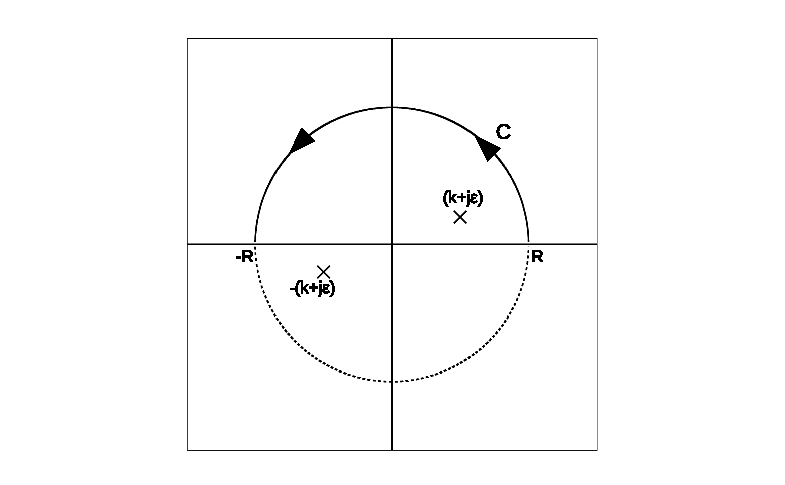
\includegraphics[width = 10cm]{./figure1new.eps}
    \label{fig1}
  \end{figure}
  \begin{eqnarray}
    F_+ = \int_{C} dk'\frac{e^{ik'(x-x')}}{(k'+k+i\epsilon)(k'-k-i\epsilon)} = \int_{-R}^Rdk' f_+(k') + \int_{C_1}dk'f_+(k')\label{c-int}
  \end{eqnarray}
  ただし
  \begin{eqnarray}
    f_+(k') = \frac{e^{ik'(x-x')}}{(k'+k+i\epsilon)(k'-k-i\epsilon)}
  \end{eqnarray}
  ここで留数定理
  \begin{eqnarray}
    \int_Cdz f(z) = 2\pi i\sum_j R(a_j)
  \end{eqnarray}
  を用いる. 極を$a_j$, Laurent展開における$(z-a)^{-n}$の係数を$R(a)$としている.今回の積分には1位の極しか含まれていないのでLaurent展開は
  \begin{eqnarray}
    R(a) = \lim_{z \rightarrow a}(z-a)f(z)
  \end{eqnarray}
  で与えられる. 以上より, (\ref{c-int})は
  \begin{eqnarray}
    F_+ &=& 2\pi i\lim_{k' \rightarrow k + j\epsilon }\left[(k'-k-j\epsilon)\frac{e^{ik'(x-x')}}{(k'+k+i\epsilon)(k'-k-i\epsilon)}\right]\\
    &=& \pi i\frac{e^{i(x-x')(k+j\epsilon)}}{k+j\epsilon}
  \end{eqnarray}
  と計算できる. さらに
  \begin{eqnarray}
    \lim_{R\rightarrow\infty}\int_{C_1}dk'f_+(k') =0
  \end{eqnarray}
  であることはすぐにわかる. 以上から
  \begin{eqnarray}
    G^\epsilon_+(x, x') &=& -\frac{1}{2\pi}\pi i\frac{e^{i(x-x')(k+j\epsilon)}}{k+j\epsilon}\\
    \therefore G_+(x, x') &=& \lim_{\epsilon\rightarrow 0}G_+^\epsilon(x, x') = -\frac{i}{2k}e^{ik(x-x')}
  \end{eqnarray}
  のように, Green関数を具体的に計算できた.\\
\item[ii)] $x<x'$の場合    
  \begin{figure}[htbp]
    \centering
    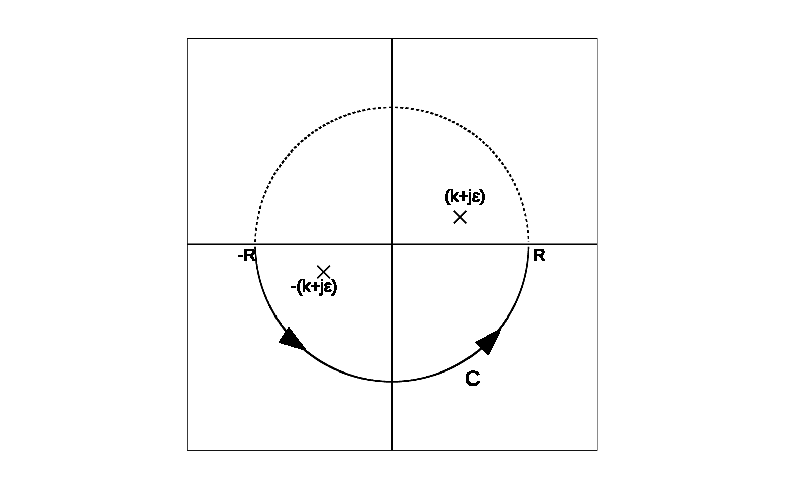
\includegraphics[width = 10cm]{./figure2new.eps}
    \label{fig2}
  \end{figure}
  先程と同様の計算より,
  \begin{eqnarray}
    G_-(x, x') = -\frac{i}{2k}e^{-ik(x-x')}
  \end{eqnarray}
  となる. 
\end{itemize}
まとめると,
\begin{eqnarray}
  G_\pm(x, x') = -\frac{i}{2k}e^{\pm ik(x-x')}
\end{eqnarray}
グリーン関数が求まったので, これを用いて波動関数を求める. 波動関数の摂動展開は
\begin{eqnarray}
  \psi(x) = \psi_0(x) + \int dx'G_+(x, x')H_p(x')\psi(x')
\end{eqnarray}
と表される.$\psi_0(x)$は非摂動解なので平面波であり, $H_p$はポテンシャルである. つまり, 領域ごとに$H_p$を変えてこの積分を計算すれば良い.
\section{場の理論におけるGreen関数}
場の理論と書きましたが, 以下では第二量子化された量子力学\footnote{「第二量子化された量子力学」と「場の量子論」は明確に区別されるべきです. 量子力学はあくまでSchr\"odinger方程式によって真空(基底状態)が決まるが, 場の量子論では真空は理論を閉じるように選ぶものである. 第二量子化における真空は消滅演算子$a$が消去する状態で確定しますが, 場の量子論においては真空期待値$\bra{0}\psi\ket{0}$がゼロでない値を持つことが許されます. こういう構造がないと, 粒子が存在する状態を真空とするBECのような物理を記述できなくなります.}におけるGreen関数についてまとめます.
\subsection{時間依存自由粒子Green関数}
場の演算子$\psi(\bm{x}, t)$はSchr\"odinger方程式
\begin{eqnarray}
  \left(i\hbar\partial_t -H\right)\psi(\bm{x}, t) = 0
\end{eqnarray}
で記述される. 今までの1粒子波動関数と同様に, 非摂動部のGreen演算子は
\begin{eqnarray}
  G_0(\bm{x}, t) = \left(i\hbar\partial_t -H_0\right)^{-1}
\end{eqnarray}
と表せ, グリーン関数は
\begin{eqnarray}
  \left(i\hbar\partial_t -H_0\right)G_0(\bm{x}, \bm{x}'; t, t') = \delta(t-t')\delta(\bm{x} - \bm{x}')
\end{eqnarray}
である. この微分方程式の解は2つ存在する:
\begin{eqnarray}
  G_0^R(k, \tau) &=& -i\theta(\tau)e^{-iE_k\tau}\hspace{1cm}\tau = t-t'\\
  G_0^A(k, \tau) &=& i\theta(\tau)e^{-iE_k\tau}\hspace{1cm}\tau = t'-t
\end{eqnarray}
$G^R$を遅延グリーン関数, $G^A$を先進グリーン関数と呼ぶ. 現象が時間に対して未来に進むのが遅延グリーン関数, 過去に進むのが先進グリーン関数になっている\footnote{数学的には時間が反転するような解を持っていてもおかしくないし, むしろ持っているべき. 時間発展がユニタリーなら解は時間反転対称性がある. }. 因果律を考慮しなくて良い場合であればどちらを用いてもよいが, 遅延グリーン関数の方が物理的な直感と合致している.
\subsection{相関関数と温度Green関数}
系が熱平衡状態にあるとき, $t = 0$の基底状態$\ket{\psi(0)}$を用いてGreen関数は, 可観測量$A, B$の時間相関関数で与えられる\footnote{Green関数が系に何かしらの揺動を与えた時の応答と解釈するなら自然な定義と言える.}:
\begin{eqnarray}
  G(t-t') \equiv \expval{\expval{A(t)B(t')}} = -i\bra{\psi(0)}{\rm T}[A(t)B(t')]\ket{0}
\end{eqnarray}
$A(t), B(t')$はHeisenberg描像, ${\rm T}[\ ]$は時間順序積. T積は因果律を守るために導入されている.

有限温度系における期待値は
\begin{eqnarray}
  \expval{A} = \frac{{\rm Tr}Ae^{-\beta H}}{{\rm Tr}e^{-\beta H}}
\end{eqnarray}
で与えられるので, 上のGreen関数は
\begin{eqnarray}
  G(t-t') &=& -i\frac{{\rm T}[{\rm Tr}A(t)B(t')e^{-\beta H}]}{{\rm Tr}e^{-\beta H}}\\
  &=& -i\frac{{\rm T}[{\rm Tr}e^{iHt/\hbar}Ae^{-iHt/\hbar}e^{iHt/\hbar}Be^{-iHt/\hbar}e^{-\beta H}]}{{\rm Tr}e^{-\beta H}}\\
  &=& -i\frac{{\rm T}[{\rm Tr}e^{iHt/\hbar}ABe^{-(it/\hbar + \beta)H}]}{{\rm Tr}e^{-\beta H}}
\end{eqnarray}
これを温度Green関数(松原Green関数)と呼ぶ.
\newpage
\chapter{超伝導}
超伝導の現象論であるGinzburg-Landau理論とBCS理論を扱う. 
\section{超電導の基礎}
\subsection{超電導体の性質}
\begin{itemize}
\item 電気抵抗ゼロ
\item 磁束の侵入を許さない (flux exclusion)
\item 磁束の排除が起こる (flux expulsion)
\end{itemize}
超伝導でない抵抗ゼロの金属ではflux expulsionはない.
\subsection{磁束の量子化}
磁束の量子化は超伝導の巨視波動関数$\psi = \psi_0e^{i\theta}$の一価性の要請から導かれる.
\begin{eqnarray}
  \nonumber  \bm{J}_s &=& \frac{e}{2m}\frac{\hbar}{i}(\psi^*\nabla) - \frac{e^2}{m}|\psi|^2\bm{A}\\
  &=& -\frac{e}{m}|\psi|^2(\hbar\nabla\theta + e\bm{A})
\end{eqnarray}
$\bm{J}_s ~ n_se\bm{v}_s = |\psi|^2e\bm{v}_s$であることに着目すると
\begin{eqnarray}
  \nabla\theta = -\frac{m}{\hbar}\bm{v}_s - \frac{e}{\hbar}\bm{A}
\end{eqnarray}
となる. 波動関数の一価性が保証されるには, 閉曲面$C$に沿って線積分したものが$2\pi$の整数倍でなければならない:
\begin{eqnarray}
  \int_C dl \nabla\theta = \int_C dl \bm{v}_s = 2\pi n
\end{eqnarray}
循環が量子化されている.
\section{超伝導の現象論 : Ginzburg-Landau理論}
超伝導を現象論的にモデル化したGinzburg-Landau理論について. 
\subsection{相転移とOder parameter}
ハミルトニアンが
\begin{eqnarray}
  H = -2\sum_{i,j}J\bm{s}_i\cdot\bm{s}_j
\end{eqnarray}
と書けるようなスピン相互作用を考える. これをハイゼンベルグ模型という. 系の平衡状態はHelmholtz自由エネルギー
\begin{eqnarray}
  F = U -TS
\end{eqnarray}
を最小にするように決まる. 低温($T<\!<U/S$)ならば内部エネルギー$U=\expval{H}$がleadingであり, これを最小化するようにスピンの向きが揃う. これを強磁性体と呼ぶ.  一方で高温ならばエントロピーの項が優勢なのでエントロピーが最大になるようにスピンの向きがバラバラになる. これを常磁性体と呼ぶ.

スピンの向きが揃うときに真空期待値が値を持ち, これを秩序変数と呼ぶ. 秩序変数がゼロでない値に変化するとき, これを相転移と呼ぶ.
\subsection{Ginzburg-Landau方程式}
自由エネルギーを秩序変数$\psi$の冪で展開:
\begin{eqnarray}
  {\cal F}[\psi] = {\cal F}_0 + \alpha|\psi|^2 + \frac{\beta}{2}|\psi|^4
\end{eqnarray}
ここで$\alpha = a(T-T_C)$である. 自由エネルギーの最小を与える$|\psi|$は微分すれば
\begin{eqnarray}
  |\psi| =
  \begin{cases}
    \hspace{1cm}0&(T>T_C)\\
    \\
    \sqrt{\cfrac{a(T_C-T)}{\beta}}&(T<T_C)
  \end{cases}
\end{eqnarray}
と求められる. そもそも$|\psi| = M$(磁化)と考えるのが自然で, なおかつ時間反転対称性を持っているので$M$の奇数次はない. $\alpha<0$のときに$|\psi| = 0$以外の極値を持つようになる. $\alpha(T) = a(T-T_C)$とすれば相転移を記述できる.

$\psi$が空間一様でない, つまり$\psi$が$r$依存性を持つ場合は
\begin{eqnarray}
  {\cal F} &=& {\cal F}_0 + \int d\bm{r} f(\bm{r})\\
  &=& {\cal F}_0 + \int dV\left[\alpha|\psi(\bm{r})|^2 + \frac{\beta}{2}|\psi(\bm{r})|^4\right]  
\end{eqnarray}
と書くことにする. 外部磁場などがある場合, 粒子の運動エネルギ^による補正項を加えなければならない:
\begin{eqnarray}
  \int dV \frac{\hbar^2}{2m}|\nabla\psi(\bm{r})|^2
\end{eqnarray}
自由エネルギーにはゲージ対称性があるので, ゲージ変換に対して不変な形で導入しなければならない:
\begin{eqnarray}
  {\cal F} &=& {\cal F}_0 + \int dV\left[\frac{\hbar^2}{2m}\left|\left(\nabla - \frac{ie}{\hbar}\bm{A}(\bm{r}))\psi(\bm{r}\right)\right|^2 + \alpha|\psi(\bm{r})|^2 + \frac{\beta}{2}|\psi(\bm{r})|^4 + \frac{\mu_0}{2}(\nabla\times\bm{A})^2\right]
\end{eqnarray}
これの変分がゼロになるところを探す:
\begin{eqnarray}
  \nonumber  \delta{\cal F} &=&\int dV\left[-\frac{\hbar^2}{2m}\left(\nabla - \frac{ie}{\hbar}\bm{A}(\bm{r})\right)^2\psi(\bm{r}) + \alpha\psi(\bm{r}) + \beta|\psi(\bm{r})|^2\psi(\bm{r})\right]\delta\psi^*(\bm{r})\\
  &+&\int \left[\frac{\hbar^2}{2m}\left(\nabla - \frac{ie}{\hbar}\bm{A}(\bm{r})\right)\psi(\bm{r})\right]\delta\psi^*(\bm{r})\cdot d\bm{S}
\end{eqnarray}
右辺第一項の被積分関数がゼロになることから
\begin{eqnarray}
  \left[-\frac{\hbar^2}{2m}\left(\nabla - \frac{ie}{\hbar}\bm{A}(\bm{r})\right)^2 + \alpha + \beta|\psi(\bm{r})|^2\right]\psi(\bm{r}) = 0\label{GL}
\end{eqnarray}
を得る. これが秩序変数を記述するGinzburg-Landau(GL)方程式である. ちなみに今回は${\cal F}$について$\psi$の変分を取ったが, $A$についての変分を取るとアンペールの法則が出てくる.
\subsection{ゲージ変換の復習}
\subsubsection{Maxwell方程式}
電磁気学におけるゲージ変換のおはなし. Maxwell方程式
\begin{eqnarray}
  {\rm rot} \bm{E} + \frac{\partial\bm{B}}{\partial t} &=& 0\hspace{2cm}(ファラデーの法則)\\
  {\rm rot} \bm{B} - \varepsilon_0\mu_0\frac{\partial \bm{E}}{\partial t} &=& \mu_0 \bm{i}\hspace{2cm}(アンペールの法則)\\
  {\rm div} \bm{E} &=& \frac{\rho}{\varepsilon_0}\hspace{2cm}(電荷のガウスの法則)\\
  {\rm div} \bm{B} &=& 0\hspace{2cm}(電荷のガウスの法則)
\end{eqnarray}
について. $\bm{B} = {\rm rot}\bm{A}$という仮定をすると${\rm div}\bm{B} = {\rm div\ rot}\bm{A} = 0$という関係が自明に出てくる(ただし, これは$\bm{A}$に特異点がない場合). この仮定をファラデーの法則に代入:
\begin{eqnarray}
  {\rm rot}(\bm{E} + \frac{\partial \bm{A}}{\partial t}) = 0
\end{eqnarray}
もし
\begin{eqnarray}
  \bm{E} + \frac{\partial \bm{A}}{\partial t} = -{\rm grad}\phi \hspace{0.5cm}\Longrightarrow\hspace{0.5cm} \bm{E} = -{\rm grad}\phi - \frac{\partial \bm{A}}{\partial t}
\end{eqnarray}
という仮定をすればファラデーの法則も自明となる. $\phi$と$A$が導入できればMaxwell方程式がとてもカンタンになる. $\phi$と$A$をまとめて電磁ポテンシャルと呼ぶ. 新しい方程式は
\begin{eqnarray}
  \left(\nabla^2 - \varepsilon_0\mu_0\frac{\partial^2}{\partial t^2}\right)\bm{A} - {\rm grad}\left({\rm div}\bm{A} + \varepsilon_0\mu_0\frac{\partial \phi}{\partial t}\right) &=& -\mu_0\bm{i}\label{max1}\\
  \nabla^2\phi + {\rm div}\frac{\partial \bm{A}}{\partial t} &=& -\frac{\rho}{\varepsilon_0}\label{max2}
\end{eqnarray}
となる.ここで
\begin{eqnarray}
  \bm{A}' = \bm{A} + {\rm grad}\chi
\end{eqnarray}
という量を定義しても, 磁束密度$\bm{B}$は変わらない. その代わり電場は変わってしまうので
\begin{eqnarray}
  \phi' = \phi - \frac{\partial \chi}{\partial t}
\end{eqnarray}
を導入すると全て辻褄が合う. この$(\phi, \bm{A})\mapsto(\phi', \bm{A}')$の変換をゲージ変換と呼び, Maxwell方程式はゲージ不変性を持つ.
\subsubsection{ローレンツゲージ}
(\ref{max1})(\ref{max2})には各々$\phi, \bm{A}$が含まれているので計算がめんどくさい. せめて
\begin{eqnarray}
  {\rm div}\bm{A} + \varepsilon_0\mu_0\frac{\partial \phi}{\partial t} = 0\label{max3}
\end{eqnarray}
となってくれれば(\ref{max1})は
\begin{eqnarray}
  \left(\nabla^2 - \varepsilon_0\mu_0\frac{\partial \phi}{\partial t}\right)\bm{A} = -\mu_0\bm{i}\label{max4}
\end{eqnarray}
のように$\bm{A}$だけの式になり, (\ref{max3})を(\ref{max2})に代入すると
\begin{eqnarray}
  \left(\nabla^2 - \varepsilon_0\mu_0\frac{\partial^2}{\partial t^2}\right)\phi &=& -\frac{\rho}{\varepsilon_0}
\end{eqnarray}
という対称性のとてもよい形になる. (\ref{max3})をローレンツ条件という.
\begin{itembox}[c]{ローレンツゲージにおけるMaxwell方程式}
  \begin{eqnarray}
    \nonumber    \left(\nabla^2 - \varepsilon_0\mu_0\frac{\partial \phi}{\partial t}\right)\bm{A} &=& -\mu_0\bm{i}\\
    \nonumber    \left(\nabla^2 - \varepsilon_0\mu_0\frac{\partial^2}{\partial t^2}\right)\phi &=& -\frac{\rho}{\varepsilon_0}
  \end{eqnarray}
  ただし
  \begin{eqnarray}
    \nonumber    {\rm div}\bm{A} + \varepsilon_0\mu_0\frac{\partial \phi}{\partial t} = 0
  \end{eqnarray}
\end{itembox}
\begin{eqnarray}
  (\phi, \bm{A})\mapsto(\phi', \bm{A}') \Longrightarrow
  \begin{cases}
    \bm{A}' = \bm{A} + {\rm grad}\chi\\
    \phi' = \phi - \cfrac{\partial \chi}{\partial t}
  \end{cases}
\end{eqnarray}

がローレンツ条件(\ref{max3})を満たすような$\chi$が存在すれば, この以上の変形が正当化される. ローレンツゲージによるMaaxwell方程式はローレンツ共変である. 
\subsubsection{クーロンゲージ}
ローレンツ条件に対して
\begin{eqnarray}
  {\rm div}\bm{A} = 0
\end{eqnarray}
という条件を課すと, クーロンの法則と等価なポアソン方程式が導かれることからこれをクーロン条件(クーロンゲージ)と呼ぶ.
\begin{itembox}[c]{クーロンゲージにおけるMaxwell方程式}
  \begin{eqnarray}
    \nonumber   && \nabla^2\phi = -\frac{\rho}{\varepsilon_0}\\
    \nonumber    &&\nabla^2\bm{A} -\varepsilon_0\mu_0\frac{\partial^2 \bm{A}}{\partial t^2} - \varepsilon_0\mu_0\frac{\partial}{\partial t}{\rm grad}\phi = \mu_0\bm{i}
  \end{eqnarray}
  ただし
  \begin{eqnarray}
    \nonumber    {\rm div}\bm{A} = 0
  \end{eqnarray}
\end{itembox}
クーロンゲージはローレンツ共変ではなくあまり方程式の対称性は良くないが, 電磁場の量子化などでは便利なので用いられることがある.
\subsection{GLコヒーレンス長と侵入長}
外部磁場がない場合の一次元GL方程式(\ref{GL})を境界条件$\psi(0) = 0$のもとで解く:
\begin{eqnarray}
  \left[-\frac{\hbar^2}{2m}\frac{d^2}{dx^2} + \alpha + \beta|\psi(x)|^2\right]\psi(x) = 0  
\end{eqnarray}
これは$x = 0$の境界には超伝導体はなく, $x > 0$を超電導体で占められているような状況である. コヒーレンス長$/xi$を
\begin{eqnarray}
  \xi^2 = \frac{\hbar^2}{2m|\alpha|}
\end{eqnarray}
と定義する. 超伝導状態では$\alpha < 0$である\footnote{こうしないとGLヘルムホルツエネルギーが$\psi>0$の領域で最小値を持たなくなる.}. 両辺を$\psi_0 = \sqrt{|\alpha|/\beta}$を用いて整理して
\begin{eqnarray}
  -\frac{d^2\psi}{dx^2} - \psi + \psi^3 = 0
\end{eqnarray}
を得る. 左辺に$2\frac{d\psi}{dx}$を掛ける:
\begin{eqnarray}
  2\frac{d\psi}{dx}\left[-\frac{d^2\psi}{dx^2} - \psi + \psi^3\right] = 0
\end{eqnarray}
ここで
\begin{eqnarray}
  \frac{d}{dx}\left(\frac{d\psi}{dx}\right)^2 = 2\frac{d\psi}{dx}\left(\frac{d^2\psi}{dx^2}\right), \hspace{0.5cm}\frac{d\psi^2}{dx} = 2\psi\frac{d\psi}{dx}, \hspace{0.5cm}\frac{d\psi^4}{dx} &=& 4\psi^3\frac{d\psi}{dx}
\end{eqnarray}
を用いて変形する:
\begin{eqnarray}
  \frac{d}{dx}\left[-\xi^2\left(\frac{d\psi}{dx}\right)^2-\psi^2 + \frac{1}{2}\psi^4\right] = 0
\end{eqnarray}
微分がゼロなので微微分関数は定数:
\begin{eqnarray}
  -\xi^2\left(\frac{d\psi}{dx}\right)^2-\psi^2 + \frac{1}{2}\psi^4 = A\ ({\rm const})
\end{eqnarray}
また, 境界条件$d\psi/dx\rightarrow 0, \psi\rightarrow 1\ (x\rightarrow+\infty)$を課すと$A = -\frac{1}{2}$であることがわかる. これにより
\begin{eqnarray}
  \xi^2\left(\frac{d\psi}{dx}\right)^2 = \frac{1}{2}\left(1-\psi^2\right)
\end{eqnarray}
という方程式が得られる.

これは非線形微分方程式だが特解を持っている:
\begin{eqnarray}
  \psi(x) = \tanh(\frac{x}{\sqrt{2\xi}})
\end{eqnarray}
これはソリトン解と呼ばれる. $x = 0$で強制的にゼロにされた$\psi$が$\xi$程度で回復している.また
\begin{eqnarray}
  \xi = \left(\frac{\hbar^2}{2m|\alpha|}\right)^{\frac{1}{2}} = \left(\frac{\hbar^2}{2ma(T-T_C)}\right)^{\frac{1}{2}} = \left(\frac{\hbar^2}{2maT_C}\right)^{\frac{1}{2}}\left(1 - \frac{T}{T_C}\right)^{\frac{1}{2}}
\end{eqnarray}
$T\rightarrow T_C\ (T_C > T)$でコヒーレンス長は発散していく自然な結果が得られる.
\subsection{ソリトンの特徴}
普通の線形波なら波動方程式で記述される異なる波長を持つ波の重ね合わせで記述できる. 異なる波長の波は$v = f\lambda$に従って伝搬速度も異なるので, 波束は次第に崩壊していく(分散が発散していく). しかしソリトンはある非線形微分方程式の定常解なので形を変えずに伝搬していき, 波束も崩壊しない.
\section{超伝導の微視的理論 : Bardeen-Cooper-Schrieffer理論}
\subsection{金属の基本性質}
一辺$L$の箱に閉じ込められた自由電子について考える. 周期境界条件を課すと, 波動関数は平面波で記述できる:
\begin{eqnarray}
  \psi_{\bm{k}}(\bm{r}) = \frac{1}{\sqrt{L^3}}e^{i\bm{k}\cdot\bm{r}}
\end{eqnarray}
エネルギー分散関係は
\begin{eqnarray}
  \varepsilon_{\bm k} = \frac{\hbar^2k^2}{2m}
\end{eqnarray}
である. ここで波数は
\begin{eqnarray}
  k_i = n_i\left(\frac{2\pi}{L}\right)\hspace{0.5cm}(i= x, y, z)
\end{eqnarray}
で与えられる. 3次元$k$空間の単位体積$(2\pi/L)^3$あたりに1つ(スピン自由度を考えると2つ)の状態が入れる. 下の準位から埋めていくと, 状態が埋まった空間は球になる. これをフェルミ球と呼び, その境界をフェルミ面と呼ぶ. フェルミ面の半径を$k_F$とすると
\begin{eqnarray}
  N = 2\left(\frac{L}{2\pi}\right)^3\times\frac{4}{3}\pi k_F^3
\end{eqnarray}
である. 電子密度を$n = N/L^3$とすると
\begin{eqnarray}
  k_F = (3\pi n)^{\frac{1}{3}}
\end{eqnarray}
となる. エネルギー$\varepsilon$の状態を電子が占める確率はFermi-Dirac分布関数
\begin{eqnarray}
  f(\varepsilon) = \frac{1}{\exp[(\varepsilon- \varepsilon_F)/k_BT]+1}
\end{eqnarray}
で与えられる.
\subsection{電子-格子間相互作用}
電子と金属イオンの間の相互作用は電子がイオン構造を歪めるという描像で理解される\footnote{金属イオン中に電子があると電子と金属イオンが引力相互作用で近づき合い, 金属イオンの配列が微妙に歪むことになる. この電子が金属中を移動すると, 金属イオンの配列の歪みも一緒に伝搬していくように見える. これが格子振動であり, これを量子化するとフォノンになる. さて, この場合は電子の運動エネルギーが格子振動に一部持って行かれることになり, これが電気抵抗の由来になる. しかし, この電子の近くに別の電子がある場合は, 格子振動により正電荷密度が大きくなっているところからさらに引力相互作用を受けて加速することができる. つまり, ある電子が創りだした格子振動エネルギーを別の電子が受け取る, というメカニズムである. もちろんこれば古典的な描像であり, 全ての格子振動エネルギーが別の電子に引き継がれることは一見なさそうだが, 格子振動を量子化したフォノンであればdescreteなエネルギーのやりとりしかできないことになるので, 電子がフォノンのやりとりをすることでエネルギーの散逸を防ぐ枠組みを正当化することができそうである. このフォノンのやり取りをする電子の組をCooper-pairという. }. つまり, 電子がフォノンを放出して異なる波数を持つモードへ遷移する, という描像である. フォノンを介した2電子間相互作用とは, 波数$k_1, k_2$の電子が$k_1 - q, k_2 + q$となる過程である.

\begin{figure}[htbp]
  \begin{minipage}{0.5\hsize}
    \centering
    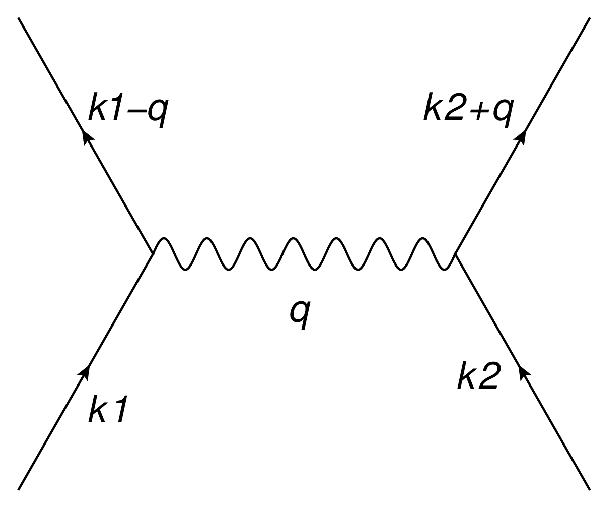
\includegraphics[width = 5.5cm]{./newdiagram1.eps}
    \figcaption{$\bm{k}_1$がフォノン$\bm{q}$を放出する過程}
    \label{diagram1}
  \end{minipage}
  \begin{minipage}{0.5\hsize}
    \centering
    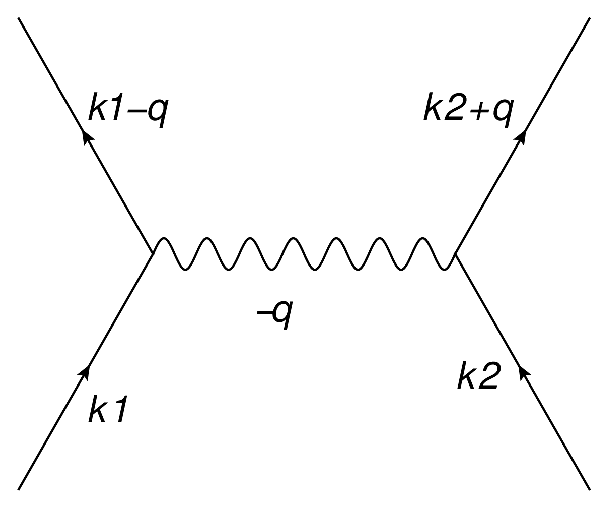
\includegraphics[width = 5.5cm]{./newdiagram2.eps}
    \figcaption{$\bm{k}_1$がフォノン$\bm{-q}$を吸収する過程}
    \label{diagram2}
  \end{minipage}
\end{figure}
フォノンを介した相互作用ハミルトニアンを$H'$とすると, エネルギーの2次摂動は
\begin{itemize}
\item 同じ電子がフォノンを放出して吸収した場合は自己エネルギー
\item 異なる電子同士がフォノンのやりとりをした場合は相互作用
\end{itemize}
を表すことになる. さて, 上の2種類の過程を考慮すると相互作用項の期待値は
\begin{eqnarray}
  U_2 &=& \sum_m\frac{\bra{f}H'\ket{m}\bra{m}H'\ket{i}}{E_i-E_m}\\
  E_i &=& \varepsilon_{\bm{k}_1} +\varepsilon_{\bm{k}_2}\\
  E_m &=&
  \begin{cases}
    \varepsilon_{\bm{k}_1 - \bm{q}} +\varepsilon_{\bm{k}_2} + \hbar\omega_{\bm{q}}\\
    \varepsilon_{\bm{k}_1} +\varepsilon_{\bm{k}_2 + \bm{q}} + \hbar\omega_{\bm{q}}
  \end{cases}
\end{eqnarray}
より
\begin{eqnarray}
  U_2 &=& \frac{|V_{\bm q}|^2}{\varepsilon_{\bm{k}_1 - \bm{q}} +\varepsilon_{\bm{k}_1} + \hbar\omega_{\bm{q}}} + \frac{|V_{\bm q}|^2}{\varepsilon_{\bm{k}_2} +\varepsilon_{\bm{k}_2 + \bm{q}} + \hbar\omega_{\bm{q}}}\\
  &=& \frac{2|V_{\bm q}|\hbar\omega_{\bm q}}{(\varepsilon_{\bm{k}_1 - \bm{q}} +\varepsilon_{\bm{k}_1})^2-(\hbar\omega_{\bm q})^2}
\end{eqnarray}
となる. ここではエネルギー保存則を用いた. $|\varepsilon_{\bm k} - \varepsilon_{\bm k-q}| <\!< \hbar\omega_{\bm q}$であれば電子間相互作用は引力となる. つまり, フェルミ面上の電子間にはフォノンを介した引力相互作用が働く可能性がある.
\subsection{Cooper問題}
次に問題になるのが, 「フェルミ面直上にある2つの電子間相互作用を考えるとき, この電子対が束縛状態を作るか」ということ. 言い換えると, 「いかに弱くても引力相互作用があれば電子対の束縛状態が実現するかどうか」. 着目する2電子の波動関数を
\begin{eqnarray}
  \Psi(\bm{r}_1, \sigma_1, \bm{r}_2, \sigma_2) = \psi(\bm{r}_1, \bm{r}_2)\chi(\sigma_1, \sigma_2)
\end{eqnarray}
とする. $\psi$が満たすのはScr\"odinger方程式
\begin{eqnarray}
  &&\bqty{-\frac{\hbar^2}{2m}\pqty{\nabla^2_1 + \nabla^2_2} + V(\bm{r}_1, \bm{r}_2)}\psi(\bm{r}_1, \bm{r}_2) = E\psi(\bm{r}_1, \bm{r}_2)\\
  &&\chi(\sigma_1, \sigma_2) = \frac{1}{\sqrt{2}}\pqty{\ket{\uparrow}\ket{\downarrow} - \ket{\downarrow}\ket{\uparrow}}
\end{eqnarray}
重心・相対座標$\bm{R} = \pqty{\bm{r}+\bm{r}}/2,\ \bm{r} = \bm{r}_1 - \bm{r}_2$を用いて
\begin{eqnarray}
  \psi(\bm{r}_1,\bm{r}_2) = \varphi(\bm{r})e^{i\bm{KR}}
\end{eqnarray}
\newpage
\chapter{Anderson局在とその周辺}
\section{Anderson局在とは}
不純物がある系において, Drudeの電子論などでは説明できない電気伝導度が実験的に確かめられた. 具体的には, Drudeモデルでは電気伝導度は平均自由行程に比例するはずだが, ある点を境に相転移のごとく電気伝導度が落ち込む結果が得られた\footnote{Anderson転移と呼ぶ}.

Andersonはこの不純物による電子の局在という問題に対して新しい理論を作った.
\section{P.W.Anderson. Phys. Rev. $\bm{109}$, 1492(1958)}
\subsection{Tight-Binding近似}
電子が規則正しい格子の上にある場合を考える. このとき電子の波動関数は原子軌道$\phi$の相対座標表示を用いて
\begin{eqnarray}
  \ket{\psi_{\bm{k}}(\bm{r})} = \sum_{\bm{R}}e^{i\bm{k}\cdot\bm{R}}\ket{\phi_0(\bm{r}-\bm{R})}
\end{eqnarray}
のように展開できる\footnote{ケットの中に位置依存性$\bm{r}$を入れる不自然さには目を瞑る方向で}. 展開係数はBroch条件を守るために平面波になっている. これがTB近似\footnote{LCAO近似とも}である.

今回は不純物が混じった系を考えるので展開系数は平面波ではない:
\begin{eqnarray}
  \ket{\psi_{\bm{k}}(\bm{r})} = \sum_{\bm{R}}a_{\bm R}^{\bm r}\ket{\phi_0(\bm{r}-\bm{R})}
\end{eqnarray}
これを各格子点のインデックスごとに和を取ることを考えて以下のように簡略化した記号を導入する:
\begin{eqnarray}
  \sum_{\bm{R}}a_{\bm R}^{\bm r}\ket{\phi_0(\bm{r}-\bm{R})} = \sum_ja_j\ket{j}
\end{eqnarray}
Schr\"odinger方程式は以下のようになる:
\begin{eqnarray}
  H\ket{\psi} &=& \qty(H_{\rm atom} + \Delta V(\bm{r}))\ket{\psi}\\
  &=&\sum_j\epsilon_j\ket{j}a_j + \sum_j\Delta V(\bm{r})\ket{j}a_j
\end{eqnarray}
$\Delta V$は全ポテンシャルから孤立原始中で電子が感じるポテンシャルを引いたもの. これの右から$\bra{i}$を作用させると
\begin{eqnarray}
  \bra{i}H\ket{\psi} = \epsilon_ia_i + \sum_jV_{ij}a_j
\end{eqnarray}
となる. $V_{ij} = \bra{i}\Delta V({\bm r})\ket{j}$であり, $\bra{i}\ket{j} \simeq \delta_{ij}$であることを用いている. 以上からハミルトニアンは
\begin{eqnarray}
  H = \sum_i\epsilon_i\ket{i}\bra{i} + \sum_{i\neq j}V_{ij}\ket{i}\bra{j}
\end{eqnarray}
であることがわかる\footnote{量子力学・場の理論ではまずハミルトニアンがあり, そこからSchr\"odinger方程式やらHeisenberg方程式やらを導出することが多いが, 今回の文脈ではその逆を行っている. つまり波動関数を作り, その波動関数でSchr\"odinger方程式を作り, ハミルトニアンを推定している. 一見不思議に思えるがこのような議論は論文でもよく見かける. 理論がSelf-consistentであればどこからスタートするかは任意であるということか}.

これらを用いて時間依存Schr\"odinger方程式
\begin{eqnarray}
  i\hbar\frac{\partial \psi_t}{\partial t} = H\psi_t
\end{eqnarray}
を時間依存性を展開系数に押し付けた波動関数の展開
\begin{eqnarray}
  \psi_t = \sum_j a_j(t)\ket{j}
\end{eqnarray}
を用いて書き換える:
\begin{eqnarray}
  i\hbar\frac{\partial a_i(t)}{\partial t} = \epsilon_ia_i(t) + \sum_{j(\neq i)}V_{ij}a_j(t)\label{schroedinger-anderson}
\end{eqnarray}
\subsection{Andersonの理論}
初期時刻にあるサイト$i=0$に電子を一つ置いて時間発展させたとき, $a_i$が時刻$\infty$で有限の値を取る場合, 電子は局在していると言える. これを計算するために(\ref{schroedinger-anderson})をLaplace変換する:
\begin{eqnarray}
  i\qty[sf_j(s) - a_j(0)] &=& \epsilon_jf_j(s) + \sum_{k(\neq j)}V_{jk}f_k(s)\\
  f_j(s) &=& \frac{i\delta_{j0}}{is - \epsilon_j} + \sum_{k(\neq j)}\frac{1}{is - \epsilon_j}V{jk}f_k(s)
\end{eqnarray}
ここでは$\hbar = 1$の単位系を用いている. また$a_j(0) = \delta_{j0}$という性質も用いている. なぜこんなことをするのかというと, $sf(s)\rightarrow a_j(\infty)\ \ (s\rightarrow 0^+)$という性質があるから. $f_j(s)$から$a_j(\infty)$の情報が得られるのである.

この右辺第二項の$f_k$に逐次代入してき, $j = 0$を代入すると
\begin{eqnarray}
\nonumber  f_0(s) &=&  \frac{i}{is - \epsilon_j} + \sum_k\frac{1}{is - \epsilon_0}V_{0k}\frac{1}{is - \epsilon_k}V_{k0}\frac{1}{is - \epsilon_0}\\
  &+& \sum_{k, m} \frac{1}{is - \epsilon_0}V{0k}\frac{1}{is - \epsilon_k}V_{km}\frac{1}{is - \epsilon_m}V_{m0}\frac{1}{is - \epsilon_0} + \cdots \label{anderson2}
\end{eqnarray}
となる. これは$j = 0$からスタートして様々な格子点を通過してまた$j = 0$に戻ってくる経路を全て足し合わせるような計算を行っている. その経路の中にはループを作るものも存在するが, 自己エネルギーは
\begin{eqnarray}
  {\cal L}_k(s) = \frac{1}{is - \epsilon_k - \varsigma}
\end{eqnarray}
というようにカウンター項$\varsigma$でくりこみが可能である. よってループのない経路のみを考えれば良い. また, コネクティビティが最近接サイト数$z$を用いて$z-2 < K \leq z - 1$と書けること, $P$ステップ後のコネクティビティが$K^P$で概算できることを用いて(\ref{anderson2})を摂動的に処理し, $a_i(\infty)$がゼロになるところと有限の値を取るところを解析したのがAndersonの1958年の論文である.

しかしこの取り扱いはなかなか難しい. これの見通しを良くするのがスケーリング理論である.
\section{E.Abrahams et al. Phys. Rev. Lett. $\bm{42}$, 673(1979)}
\newpage
\chapter{熱・統計・量子統計力学}
\section{熱力学}
\subsection{状態量}
系の状態のみで一意に決まり, 過去の履歴・経路に依らない(積分値が経路に依らない)ものを状態量と呼ぶ. 
\subsection{完全な熱力学関数}
系の平衡状態における熱力学的性質の情報を全て持っているものを完全な熱力学関数と呼ぶ. 示量性状態量. 系の情報を全て持っているというのは, 状態量がこの関数の偏微分で全て求まるということ. 例えば内部エネルギー$U(S, N, V)$を用いて
\begin{eqnarray}
  \partial_SU &=& T\\
  \partial_NU &=& \mu\\
  \partial_VU &=& -p
\end{eqnarray}
という状態量が求まる. 全微分は
\begin{eqnarray}
  dU = TdS -pdV + \mu dN
\end{eqnarray}
である. これを変形して
\begin{eqnarray}
  dS = \frac{1}{T}dU +\frac{p}{T}dV - \frac{\mu}{T} dN
\end{eqnarray}
となり, $S$は$U, V, N$を変数とする関数として表された時に完全な熱力学関数となる. 統計力学においては温度を定義するときに
\begin{eqnarray}
  \partial_US = \frac{1}{T}
\end{eqnarray}
という表式をしばしば用いる.
\subsection{自由エネルギー}
熱力学第二法則より, 系は自由エネルギーが減少する方向に遷移する. 
\subsubsection{ヘルムホルツ自由エネルギー}
等温下で仕事として取り出し可能なエネルギーを表す.ヘルムホルツエネルギーが極小値を取るとき, 系は熱平衡状態にある.

定義:
\begin{eqnarray}
  F(T, V, N) = U(S(T, V, N), V, N) -TS(T, V, N)
\end{eqnarray}
ここで現れるエントロピーは完全な熱力学関数ではない. 各変数による偏微分は
\begin{eqnarray}
  \partial_TF &=& -S\\
  \partial_VF &=& -p\\
  \partial_NF &=& \mu
\end{eqnarray}
である. 全微分は
\begin{eqnarray}
  dF = -S(T, V, N)dT -p(T, V, N)dV + \mu(T, V, N) dN
\end{eqnarray}
\subsubsection{ギブズ自由エネルギー}
等温等圧下で仕事として取り出し可能なエネルギーを表す. ヘルムホルツエネルギーとの違いは等圧条件の有無.

定義:
\begin{eqnarray}
  G(T, p, N) = U(S(T, p, N), p, N) -TS(T, p, N)
\end{eqnarray}
以下ヘルムホルツエネルギーと同様.
\section{統計力学}
\subsection{目的}
微視的状態の数をかぞえて巨視的状態を導く. 
\subsection{ミクロカノニカルアンサンブル}
\subsection{Langevin方程式}
ブラウン粒子の運動を記述する方程式としてLangevinが導入した.
\begin{eqnarray}
  M\frac{dv}{dt} = -\frac{v}{\mu} + F_{\rm ext} + R(t)\label{Langevin}
\end{eqnarray}
ここで$\mu$を移動度, $F_{ext}$をマクロな外力, $R(t)$をミクロなノイズとする. $R$が確率過程であるので, 初期条件を与えても$v$が決定論的に定まらない. 

速度をFourier変換する:
\begin{eqnarray}
  v(t) &=& \frac{1}{\sqrt{2\pi}}\int d\omega e^{-i\omega t}\tilde{v}(\omega)\label{v1}\\
  \tilde{v}(\omega) &=& \frac{1}{\sqrt{2\pi}}\int dt e^{i\omega t}v(t)\label{v2}
\end{eqnarray}
さらに速度の時間相関関数とそのFourier変換を定義する:
\begin{eqnarray}
  C_v(t) &=& \expval{v(t_0)v(t_0 + t)}\\
  \tilde{C}_v(\omega) &=& \frac{1}{\sqrt{2\pi}}\int dt'e^{i\omega't'}\expval{v(t_0)v(t_0+t')}
\end{eqnarray}
ここで$\tilde{v}^*(\omega) = \tilde{v}(-\omega)$が成立している. (\ref{v2})より
\begin{eqnarray}
  \expval{\tilde{v}(\omega)\tilde{v}^*(\omega')} &=& \frac{1}{2\pi}\int dtdt' e^{i\omega t-i\omega' t'}\expval{v(t)v(t')}\\
  &=&\frac{1}{2\pi}\int dtdt'\left|\det(J)\right| e^{i\omega t'}e^{i(\omega -\omega')t}\expval{v(t+t')v(t)}\\
  &=&\delta(\omega-\omega')\int dt'e^{i\omega' t'}\expval{v(t+t')v(t)}\\
  &=&\delta(\omega-\omega')I_v(\omega')
\end{eqnarray}
ただし
\begin{eqnarray}
  J =
  \begin{pmatrix}
    \cfrac{\partial(t+t')}{\partial t}&\cfrac{\partial(t+t')}{\partial t'}\\
    \cfrac{\partial t'}{\partial t}&\cfrac{\partial t'}{\partial t'}\\
  \end{pmatrix}\hspace{1cm} |\det(J)| = 1
\end{eqnarray}
である. この式から
\begin{eqnarray}
  I_v(\omega) = \int dtC_v(t)e^{i\omega t} = \tilde{C}(\omega)
\end{eqnarray}
がわかる. これをWiener-Khinchinの定理という. 相関関数とパワースペクトルはFourier変換を通して関係付けられる.$\tilde{R}(\omega)$についても同様のことが言える:
\begin{eqnarray}
  \tilde{R}(\omega) &=& \frac{1}{\sqrt{2\pi}}\int dt e^{i\omega t}R(t)\label{R2}\\
  \tilde{C}_R(\omega) &=& \frac{1}{\sqrt{2\pi}}\int dte^{i\omega t}\expval{R(t_0)R(t_0+t)}\\
  \expval{\tilde{R}(\omega)\tilde{R}^*(\omega')}&=& \tilde{C}_R(\omega')\delta(\omega-\omega') 
\end{eqnarray}

以降$F_{\rm ext} = 0$のもとでLangevin方程式の解析をする. (\ref{Langevin})に(\ref{v1})を代入:
\begin{eqnarray}
  M\frac{d}{dt}\int d\omega e^{-i\omega t}\tilde{v}(\omega) &=& \int d\omega e^{-i\omega t}\left(-\frac{\tilde{v}(\omega)}{\mu} + \tilde{R}(\omega)\right)  \\
  \Longleftrightarrow M(-i\omega)\tilde{v}(\omega) &=&  -\frac{\tilde{v}(\omega)}{\mu} + \tilde{R}(\omega)
\end{eqnarray}
$\gamma = (M\mu)^{-1}$とすると
\begin{eqnarray}
  \tilde{v}(\omega) = \frac{1}{-i\omega + \gamma}\frac{\tilde{R}(\omega)}{M}
\end{eqnarray}
であることがわかる. 時間相関関数は
\begin{eqnarray}
  \tilde{C}_v(\omega) &=& \int d\omega' \expval{\tilde{v}(\omega)\tilde{v}^*(\omega')} = \frac{1}{(-i\omega + \gamma)(i\omega' + \gamma)M^2}\int d\omega' \expval{R(\omega)R^*(\omega')}\\
  &=& \frac{1}{(-i\omega + \gamma)(i\omega' + \gamma)M^2}\int d\omega' \tilde{C}_R(\omega')\delta(\omega-\omega') = \frac{1}{\omega^2 + \gamma^2}\frac{\tilde{C}_R(\omega)}{M^2}
\end{eqnarray}
$R$の確率過程の性質が与えられてパワースペクトル$C_R$が定まると速度$v$の相関関数やパワースペクトルが決定される. $R$がホワイトノイズだと仮定すると,
\begin{eqnarray}
  C_R(t) = \expval{R(t_0+t)R(t_0)} = C_R\delta(t)\\
  \tilde{C}_R(\omega) = \int dt e^{-i\omega t}C_R(t) = C_R
\end{eqnarray}
ということで, $\tilde{C}_R$は$\omega$によらない定数になる. このようなノイズを仮定すると, 速度相関関数は
\begin{eqnarray}
  C_v(t) = \int d\omega e^{-i\omega t}\tilde{C}_v(\omega) = \int d\omega \frac{C_Re^{-i\omega t}}{M^2(\omega^2 + \gamma^2)}
\end{eqnarray}
この積分を実行するために複素積分の応用を用いる:
\begin{eqnarray}
  \int_C dz \frac{C_Re^{-izt}}{M^2(z^2 + \gamma^2)} = \int_{C_1} \frac{C_Re^{-izt}}{M^2(z^2 + \gamma^2)} + \int_{-R}^R \frac{C_Re^{-izt}}{M^2(z^2 + \gamma^2)}
\end{eqnarray}
\begin{figure}[htbp]
  \centering
  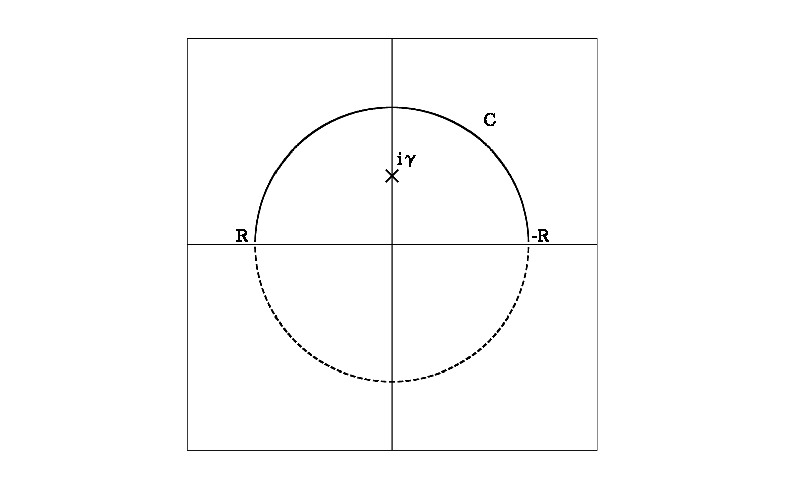
\includegraphics[width = 10cm]{./figure3new.eps}
  \label{fig3}
\end{figure}\\
極は$\omega = \pm i\gamma$で一位の極. 積分経路は上半円とする. 留数定理より
\begin{eqnarray}
  R(i\gamma) = \lim_{z\rightarrow i\gamma}(z - i\gamma)f(z) = \frac{C_Re^{\gamma t}}{2i\gamma}\label{R}
\end{eqnarray}
ここで$z = Re^{i\theta}$の変数変換を施すことにより
\begin{eqnarray}
  \int_{C_1}dz\frac{e^{-izt}}{(z^2 + \gamma^2)} = \int_0^\pi d\theta\frac{iRe^{-iRe^{i\theta}}t}{(R^2e^{2i\theta} + \gamma^2)}= \int_0^\pi d\theta\frac{iRe^{-iRt\cos\theta}e^{Rt\sin\theta}}{(R^2e^{2i\theta} + \gamma^2)}
\end{eqnarray}
かつ一般に$|\alpha + \beta| > |\alpha|-|\beta|$が成立することから
\begin{eqnarray}
  \left|\frac{iRe^{-iRt\cos\theta}e^{Rt\sin\theta}}{(R^2e^{2i\theta} + \gamma^2)}\right| < \frac{Re^{Rt\sin\theta}}{R^2 - \gamma^2}
\end{eqnarray}
これが$R\rightarrow\infty$で発散しないためには$t<0$である必要があるが, $t>0$の場合も発散しないようにしたい. そのためには$e^{-izt}\rightarrow e^{iz|t|}$とすればよい. つまり, (\ref{R})は
\begin{eqnarray}
  R(i\gamma) = \lim_{z\rightarrow i\gamma}(z - i\gamma)f(z) = \frac{C_Re^{-\gamma |t|}}{2i\gamma}\label{R2}
\end{eqnarray}
とするべきである. 以上からコーシーの積分定理より
\begin{eqnarray}
  C_v(t) = \frac{C_Re^{-\gamma|t|}}{2M^2\gamma}
\end{eqnarray}
となる. 同時刻($t = 0$)の相関は
\begin{eqnarray}
  C_v = \frac{C_R}{2M^2\gamma}
\end{eqnarray}
であり, 熱平衡状態のエネルギー等分配則
\begin{eqnarray}
  M\expval{v^2} = k_BT
\end{eqnarray}
を認めれば
\begin{eqnarray}
  C_R = 2k_BTM\gamma
\end{eqnarray}
となる. これはNyquistの定理と呼ばれ, 揺動散逸定理のひとつである.
\section{Born-Markov型量子マスター方程式}
熱浴と接している一次元調和振動子系のBorn-Markov型量子マスター方程式を解く.
\begin{itemize}
\item 系のハミルトニアンは調和振動子$H = \hbar\omega a^\dagger a$.
  
\item Born-Markov近似なので熱浴の密度演算子は時間発展せず, 回転波近似(弱結合)も有効.
  
\item マスター方程式は系の密度演算子の時間発展を与えている.\footnote{描像によっては生成消滅演算子も時間依存しそうである. 普通(?)マスター方程式を導出するときは相互作用描像を経由するので生成消滅演算子も一般に時間依存性を持つ. しかし今回は回転波近似が有効であるため, $a(t) = a(0)e^{-i\omega t}$のように分解できる. 後述のマスター方程式には$a^\dagger$, $a$がペアになって現れているので, マスター方程式には生成消滅演算子に依る時間依存性は現れない. $a^\dagger$, $a$がペアになっていないような項が現れたら生成消滅演算子由来の時間依存性を考慮しなければならないが, そもそもそういう項を落とすのがBorn-Markov近似である. }.
\end{itemize}
\begin{itemize}
\item 生成消滅演算子と粒子数状態
  
\item 交換関係の計算  
\end{itemize}
あたりの知識が必要です.
\subsection{問題設定}
量子マスター方程式が与えられている:
\begin{eqnarray}
  \nonumber  \partial_t\rho(t) = &-&i\omega[a^\dagger a, \rho(t)] + \kappa\overline{n}(2a^\dagger\rho(t)a - aa^\dagger\rho(t) - \rho(t)aa^\dagger)\\
  &+&\kappa(\overline{n} + 1)(2a\rho(t)a^\dagger - a^\dagger a\rho(t) - \rho(t)a^\dagger a)\label{master}
\end{eqnarray}
ただし
\begin{eqnarray}
  \kappa > 0,\hspace{1cm} \overline{n} = \frac{1}{e^{\hbar\omega/kT}-1},\hspace{1cm} [a, a^\dagger] = 1
\end{eqnarray}
であり, $\kappa$は減衰定数, $\overline{n}$はBose-Einstein分布関数, $a, a^\dagger$は生成消滅演算子である.
\subsection{熱平衡(問題1)}
熱浴の温度が$T$であることから, 系の温度を$T$とする有限温度系を考えればそれが熱平衡状態にあることは明らか. 平衡状態なので密度演算子が系のハミルトニアンを用いて
\begin{eqnarray}
  \rho_{th} = \frac{e^{-H/kT}}{{\rm Tr}e^{-H/kT}}\label{equiliblium}
\end{eqnarray}
と書ける. (\ref{equiliblium})の分母は規格化条件であり,以下のように計算できる\footnote{トレースは直行完全系ではさんで和を取ればいい.規格化は後でできるので, 正規直行完全系でなくてもいいらしい. つまりどんな完全系を選んできても規格化係数を除けば同じ結論に辿り着く. 今回は明らかに$a^\dagger a$の固有状態$\ket{n}$を用いるのが簡単. }(以下, 逆温度$1/kT$を$\beta$と置き換えています):
\begin{eqnarray}
  \nonumber  {\rm Tr}e^{-\beta\hbar\omega a^\dagger a} &=& \sum_{n}\bra{n}e^{-\beta\hbar\omega a^\dagger a}\ket{n}\\
  \nonumber  &=& \sum_{n}e^{-\beta\hbar\omega n}\\
  &=& \frac{1}{1-e^{-\beta\hbar\omega}} = (\overline{n} -1)
\end{eqnarray}

密度演算子はLiouville-von Neumann方程式を満たす:
\begin{eqnarray}
  i\hbar\partial_t\rho_{th} &=& [H, \rho_{th}]\\
  &=& \frac{\hbar\omega}{\overline{n}-1}[a^\dagger a, e^{\beta\hbar\omega a^\dagger a}]\label{commutation}
\end{eqnarray}
$[A, [B, A]] = [B, [B, A]] = 0$が成立しているときに$[B, e^{\lambda A}] = \lambda[B, A]e^{\lambda A}$であることを利用して\footnote{証明してみよう!}
\begin{eqnarray}
  (\ref{commutation}) = \frac{\hbar\omega}{\overline{n}-1}\beta\hbar\omega[a^\dagger a, a^\dagger a]e^{\beta\hbar\omega a^\dagger a} = 0
\end{eqnarray}
したがって, $\rho_{th}$の時間微分がゼロであることから時間発展しない熱平衡状態であることがわかる\footnote{式(\ref{master})を使っていないが良いのか?と思うかもしれないが, そもそも量子マスター方程式を導出するときはLiouville-von Neumann方程式からスタートするので, QME$\subset$LvNEである}.
\subsection{調和振動子のエネルギー(問題2)}
続いて式(\ref{master})を用いてエネルギー期待値の時間発展を追う.物理量の期待値はハミルトニアンに密度演算子を掛けてトレースアウトすればよい\footnote{本来, 密度演算子を用いた物理量の期待値は$\expval{A} = \frac{{\rm Tr}A\rho(t)}{{\rm Tr}\rho(t)}$で記述されるが, 今回は${\rm Tr}\rho(t) = 1$を課している.つまり$\rho(t)$が規格化されているという条件である.}:
\begin{eqnarray}
  \partial_tE(t) = \partial_t{\rm Tr}[H\rho(t)] = \hbar\omega\partial_t\sum_n \bra{n}a^\dagger a\rho(t)\ket{n} = \hbar\omega\partial_t\sum_nn\bra{n}\rho(t)\ket{n}\label{4.1}
\end{eqnarray}
また, 式(\ref{master})に左から$H = \hbar\omega a^\dagger a$を掛けてトレースアウトする:
\begin{eqnarray}
  \nonumber  \partial_tE(t) = &-&i\hbar\omega^2\underline{{\rm Tr}\left(a^\dagger a[a^\dagger a, \rho(t)]\right)}_{\rm 1} + \kappa\overline{n}\hbar\omega\left(2\underline{{\rm Tr}a^\dagger aa^\dagger\rho(t)a}_{\rm 2} - \underline{{\rm Tr}a^\dagger a aa^\dagger\rho(t)}_{\rm 3} - \underline{{\rm Tr}a^\dagger a\rho(t)aa^\dagger}_{\rm 4}\right)\\
  &+&\kappa(\overline{n} + 1)\hbar\omega\left(2\underline{{\rm Tr}a^\dagger aa\rho(t)a^\dagger}_5 - \underline{{\rm Tr}a^\dagger aa^\dagger a\rho(t)}_6 - \underline{{\rm Tr}a^\dagger a\rho(t)a^\dagger a}_7\right)\label{ModifiedMaster}
\end{eqnarray}
式(\ref{ModifiedMaster})の右辺は,
\begin{eqnarray}
  \nonumber  1.\hspace{5mm}{\rm Tr}\left(a^\dagger a[a^\dagger a, \rho(t)]\right) &=& {\rm Tr}\left[a^\dagger a(a^\dagger a\rho(t)-\rho(t)a^\dagger a)\right]\\
  \nonumber  &=&\sum_n\left[\bra{n}a^\dagger aa^\dagger a\rho(t)\ket{n} - \bra{n}a^\dagger a\rho(t)a^\dagger a\ket{n}\right]\\
  &=&\sum_n\left[n^2\bra{n}\rho(t)\ket{n} - n^2\bra{n}\rho(t)\ket{n}\right] = 0\\
  2.\hspace{5mm}{\rm Tr}a^\dagger aa^\dagger\rho(t)a &=& \sum_n(n+1)^2\bra{n}\rho(t)\ket{n}\\
  3.\hspace{5mm}{\rm Tr}a^\dagger aaa^\dagger\rho(t) &=& \sum_nn(n+1)\bra{n}\rho(t)\ket{n}\\
  4.\hspace{5mm}{\rm Tr}a^\dagger a\rho(t)aa^\dagger &=& \sum_nn(n+1)\bra{n}\rho(t)\ket{n}\\
  5.\hspace{5mm}{\rm Tr}a^\dagger aa\rho(t)a^\dagger &=& \sum_n(n-1)n\bra{n}\rho(t)\ket{n}\\
  6.\hspace{5mm}{\rm Tr}a^\dagger aa^\dagger a\rho(t) &=& \sum_nn^2\bra{n}\rho(t)\ket{n}\\
  7.\hspace{5mm}{\rm Tr}a^\dagger a\rho(t)a^\dagger a &=& \sum_nn^2\bra{n}\rho(t)\ket{n}
\end{eqnarray}
用いて整理することができる\footnote{nの和については$n=0$とか$n=\infty$の境界を雑に扱っているように見えるが, ちゃんとDirichlet境界条件を考慮してあげれば問題は起きない(と思う)}:
\begin{eqnarray}
  \nonumber \partial_tE(t) &=& \sum_n2\hbar\omega\left[\kappa\overline{n}((n+1)^2-n(n+1)) + \kappa(\overline{n}+1)((n-1)n - n^2)\right]\bra{n}\rho(t)\ket{n}\\
  &=&\sum_n2\hbar\omega\left[\kappa\overline{n}(n+1) - \kappa(\overline{n}+1)n\right]\bra{n}\rho(t)\ket{n}\\
  &=&\sum_n2\hbar\omega\kappa\left(\overline{n} - n\right)\bra{n}\rho(t)\ket{n}
\end{eqnarray}
式(\ref{4.1})と比較すると
\begin{eqnarray}
  \hbar\omega\sum_n\partial_tn\bra{n}\rho(t)\ket{n} &=& \sum_n2\hbar\omega\kappa\left(\overline{n} - n\right)\bra{n}\rho(t)\ket{n}\\
  \partial_tn\bra{n}\rho(t)\ket{n} &=& 2\kappa\left(\overline{n} - n\right) \bra{n}\rho(t)\ket{n}\\
  &\therefore& n\bra{n}\rho(t)\ket{n} = C_ne^{2\kappa\left(\frac{\overline{n}}{n} - 1\right)t}
\end{eqnarray}
よってエネルギー固有値は式(\ref{4.1})より
\begin{eqnarray}
  E(t) = \sum_n C_ne^{2\kappa\left(\frac{\overline{n}}{n} - 1\right)t}
\end{eqnarray}
となる\footnote{熱平衡状態では物理量に温度が関与していそうだが, (平衡状態ではない)非平衡の形式では系の温度が式に現れていないことを不思議に思うかもしれない. しかし, そもそも温度とは平衡状態でなければ定義できない.むしろ平衡状態によって定義される量である. 熱力学においては温度という概念が当たり前のように存在するが, そもそもは熱力学第零法則に則って熱平衡の下で定義される(熱力学は平衡状態に関する理論). つまり我々は平衡有限温度系では式(\ref{equiliblium})を用いて温度を定義することになる. この式だけでは定義のしようがないと思うかもしれないが, 場の量子論の形式においては理論を閉じるようにうまく繰り込み条件を選ぶことにより,自己無同着的に定義されることになる.}.
$C_n$は積分定数\footnote{Cがn依存性を持っていないと式(\ref{4.16})が発散してしまう.}. 初期状態$t = 0$のエネルギー平均が$E(0)$であることから
\begin{eqnarray}
  E(0) = \sum_nn\bra{n}\rho(0)\ket{n} = \sum_nC_n\label{4.16}
\end{eqnarray}
となる. 
\subsection{位置・運動量平均の時間発展(問題3)}
(問題2)と同様にマスター方程式のトレースアウトで期待値を見積もる.以下, 位置と運動量は$m=\hbar=\omega = 1$で無次元化している\footnote{マスター方程式は無次元化されていないのでアンバランスなあまり良いnotationではない. 本来ならマスター方程式, $\overline{n}$も合わせて無次元化すべき.}.

生成消滅演算子の言葉で位置は$q = \frac{1}{\sqrt{2}}(a^\dagger + a)$と表されることを用いて
\begin{eqnarray}
  \nonumber  \partial_tq(t) &=& \frac{1}{\sqrt{2}}\partial_t{\rm Tr}(a^\dagger + a)\rho(t)\\
  &=& \frac{1}{\sqrt{2}}\partial_t\sum_n\left[\sqrt{n}\bra{n-1}\rho(t)\ket{n} + \sqrt{n+1}\bra{n+1}\rho(t)\ket{n}\right]\label{Position}
\end{eqnarray}
マスター方程式の右辺をトレースアウト:
\begin{eqnarray}
  \nonumber  (\ref{master}) &\rightarrow& \frac{1}{\sqrt{2}}\Bigl[-i\omega\underline{{\rm Tr}(a^\dagger +a)(a^\dagger a\rho(t) - \rho(t)a^\dagger a)}_1\\
    \nonumber    &+& \kappa\overline{n}\left(2\underline{{\rm Tr}(a^\dagger +a)a^\dagger \rho(t)a}_2 - \underline{{\rm Tr}(a^\dagger + a)aa^\dagger \rho(t)}_3 - \underline{{\rm Tr}(a^\dagger +a)\rho(t)aa^\dagger}_4\right)\\
    &+& \kappa(\overline{n}+1)\left(2\underline{{\rm Tr}(a^\dagger +a)a\rho(t)a^\dagger}_5 - \underline{{\rm Tr}(a^\dagger + a)a^\dagger a\rho(t)}_6 - \underline{{\rm Tr}(a^\dagger +a)\rho(t)a^\dagger a}_7\right)\Bigr]\label{position}
\end{eqnarray}
各項について整理:
\begin{eqnarray}
  &1.&\hspace{5mm}\sum_n\left[-\sqrt{n}\bra{n-1}\rho(t)\ket{n}+\sqrt{n+1}\bra{n+1}\rho(t)\ket{n}\right]\\
  &2.&\hspace{5mm}\sum_n\left[(n+1)\sqrt{n}\bra{n-1}\rho(t)\ket{n}+\sqrt{n+1}(n+2)\bra{n+1}\rho(t)\ket{n}\right]\\
  &3.&\hspace{5mm}\sum_n\left[n\sqrt{n}\bra{n-1}\rho(t)\ket{n}+\sqrt{n+1}(n+2)\bra{n+1}\rho(t)\ket{n}\right]\\
  &4.&\hspace{5mm}\sum_n\left[(n+1)\sqrt{n}\bra{n-1}\rho(t)\ket{n}+\sqrt{n+1}(n+1)\bra{n+1}\rho(t)\ket{n}\right]\\
  &5.&\hspace{5mm}\sum_n\left[(n-1)\sqrt{n}\bra{n-1}\rho(t)\ket{n}+n\sqrt{n+1}\bra{n+1}\rho(t)\ket{n}\right]\\
  &6.&\hspace{5mm}\sum_n\left[(n-1)\sqrt{n}\bra{n-1}\rho(t)\ket{n}+(n+1)\sqrt{n+1}\bra{n+1}\rho(t)\ket{n}\right]\\
  &7.&\hspace{5mm}\sum_n\left[n\sqrt{n}\bra{n-1}\rho(t)\ket{n}+n\sqrt{n+1}\bra{n+1}\rho(t)\ket{n}\right]
\end{eqnarray}
式(\ref{position})をまとめる:
\begin{eqnarray}
  \nonumber (\ref{position}) &=& \frac{1}{\sqrt{2}}\sum_n\Bigl[-i\omega\left(-\sqrt{n}\bra{n-1}\rho(t)\ket{n}+\sqrt{n+1}\bra{n+1}\rho(t)\ket{n}\right)\\
    \nonumber    &&+ \kappa\overline{n}\left( \sqrt{n}\bra{n-1}\rho(t)\ket{n}+\sqrt{n+1}\bra{n+1}\rho(t)\ket{n}\right)\\
    &&+ \kappa(\overline{n}+1)\left(-\sqrt{n}\bra{n-1}\rho(t)\ket{n}-\sqrt{n+1}\bra{n+1}\rho(t)\ket{n}\right)\Bigr]\label{positon2}\\
  &=& \frac{1}{\sqrt{2}}\sum_n\Bigl[\sqrt{n}\left(i\omega - \kappa\right)\bra{n-1}\rho(t)\ket{n}-\sqrt{n+1}\left(i\omega+\kappa\right)\bra{n+1}\rho(t)\ket{n} \Bigr]
\end{eqnarray}
(\ref{Position})と比較:
\begin{eqnarray}
  \sum_n \partial_t\bra{n-1}\rho(t)\ket{n} = \sum_n (i\omega - \kappa)\bra{n-1}\rho(t)\ket{n}\\
  \sum_n \partial_t\bra{n+1}\rho(t)\ket{n} = -\sum_n (i\omega + \kappa)\bra{n+1}\rho(t)\ket{n}
\end{eqnarray}
これを解くと
\begin{eqnarray}
  \bra{n-1}\rho(t)\ket{n} &=& C_1e^{(i\omega - \kappa)t}\\
  \bra{n+1}\rho(t)\ket{n} &=& C_2e^{-(i\omega + \kappa)t}
\end{eqnarray}
以上より
\begin{eqnarray}
  q &=& \frac{1}{\sqrt{2}}\sum_n\left[\sqrt{n}C_1e^{(i\omega - \kappa)t} + \sqrt{n+1}C_2e^{-(i\omega + \kappa)t}\right]\\
  \dot{q} &=& p = \frac{1}{\sqrt{2}}\sum_n\Bigl[\sqrt{n}C_1(i\omega - \kappa)e^{(i\omega - \kappa)t}- \sqrt{n+1}C_2(i\omega + \kappa)e^{-(i\omega + \kappa)t}\Bigr]\\
  \ddot{q} &=& \dot{p} = \frac{1}{\sqrt{2}}\sum_n\Bigl[\sqrt{n}C_1(i\omega - \kappa)^2e^{(i\omega - \kappa)t}- \sqrt{n+1}C_2(i\omega + \kappa)^2e^{-(i\omega + \kappa)t}\Bigr]
\end{eqnarray}
ここでは$\dot{q} = p$であることを用いている.以上から$\dot{p}, p, q$による微分方程式を立てる\footnote{ちょっと式とにらめっこしてれば簡単}:
\begin{eqnarray}
  \dot{p} = -(\omega^2 + \kappa^2)q -2\kappa p
\end{eqnarray}

右辺第2項が速度に比例する減衰を表している.角振動数に$\kappa$が入っており, 減衰の幅が増加するほど角振動数も大きくなる. 古典的な減衰振動を摩擦のあるばねの振動と解釈する場合, 角振動数は減衰(摩擦)がない場合と変わらないはずなので, 古典と完全には対応していないように見える.
一方で, 減衰をエネルギーの散逸と捉えるならば, 低温の熱浴からの影響で角振動数が大きくなるという解釈は, 低温ではばね定数が大きくなる古典的な解釈と一致する.

きれいになったとはいえまだミスがないか不安です...
\subsection{数値計算}
問題2の和が計算しきれなかったので, 数値計算で(\ref{4.16})が本当に緩和するかどうかを確認.
\begin{figure}[htbp]
  \begin{minipage}{0.5\hsize}
    \centering
    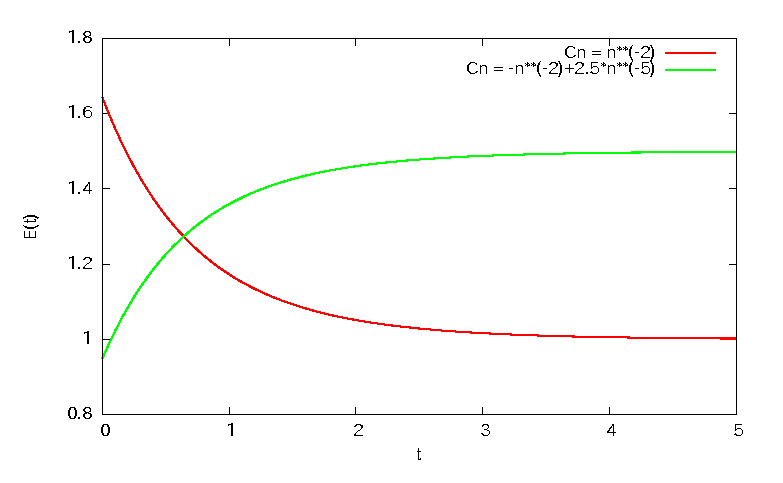
\includegraphics[width = 7cm]{./fig1.eps}
    \figcaption{$\kappa = \overline{n} = 1$}
    \label{fig1}
  \end{minipage}
  \begin{minipage}{0.5\hsize}
    \centering
    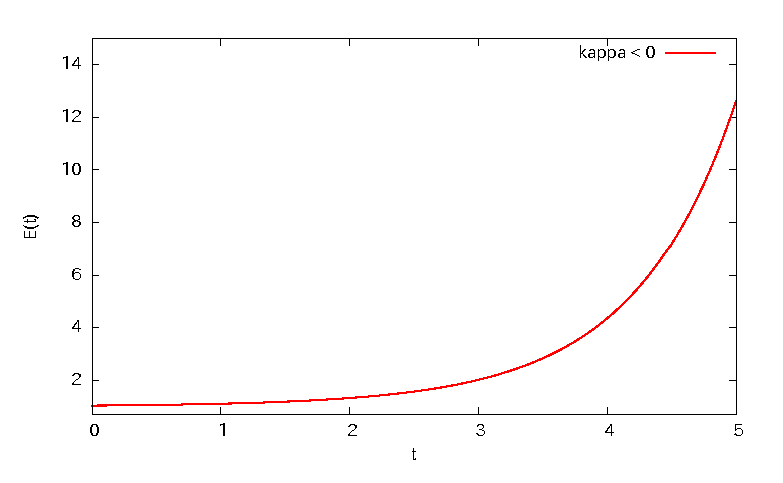
\includegraphics[width = 7cm]{./fig2.eps}
    \figcaption{$\kappa$が負の場合}
    \label{fig2}
  \end{minipage}
\end{figure}
$E(0)$の情報は$C_n$に組み込まれており, さらに$C_n$の関数列の形に制限は収束すること以外には特にない. $E(0)$は$C_n$の汎関数だとも言える. つまり, $C_n$の与え方によって熱浴を通じてエネルギーが流出するか流入するかが決まる\footnote{系の初期温度が熱浴の温度$T$より大きければ流出するし,逆なら流入するのが普通. 非平衡状態では温度は定義できないので, 正確には流入・流出を支配しているのは温度ではなくエントロピーである.}. 汎関数は無限個の自由度を持つ関数なので$E(0)$は単なる系のエネルギーの初期値だけでなく,熱浴との相関具合などの自由度を含んでいる(かもしれない). 図1にエネルギーが緩和する様子を示した.今回は$C_n = \frac{1}{n^2}, -\frac{1}{n^2} + \frac{5}{2n^5}$の2つを計算. これは単に流入と流出を見たかったために選んできたものであり, $C_n$が収束するような関数列を選べば緩和は観測できるはず.

また, $\kappa$が負の場合, 振幅は減衰することなく増幅することを図2で確認している.
\section{線形応答理論}
\subsection{概要}
ある平衡系に$t = t_0$で何かしらの外場がかかったときの非平衡過程を見る理論. 摂動1次までの応答を見るので線形応答と呼ばれる.
\subsection{線形応答理論の基本概念}
平衡系のハミルトニアンを$H$, 外場$H_{\rm ex}(t)$としてFull Hamiltonian
\begin{eqnarray}
 H_{T} = H + H_{\rm ex}(t)
\end{eqnarray}
を考える. $H_{\rm ex}(t)$は$t< t_0$においてはゼロである. 平衡系の時間依存Schr\"odinger方程式:
\begin{eqnarray}
  i\partial_t\ket{\psi(t)} = H\ket{\psi(t)}
\end{eqnarray}
に対して外場を加えたSchr\"odinger方程式:
\begin{eqnarray}
  i\partial_t\ket{\Psi(t)} = \qty(H + H_{\rm ex}(t))\ket{\Psi(t)}
\end{eqnarray}
がある. $\ket{\Psi(t)}$は非平衡系の状態である. 平衡系の形式解が
\begin{eqnarray}
  \ket{\psi(t)} = e^{-iHt}\ket{\psi(0)}
\end{eqnarray}
であることから, ユニタリー演算子を用いて$\ket{\Psi(t)}$が
\begin{eqnarray}
  \ket{\Psi(t)} = e^{-iHt}U(t)\ket{\psi(0)}
\end{eqnarray}
と書けるものとする. これをSchr\"odinger方程式に代入すると
\begin{eqnarray}
  i\partial_t U(t) = e^{iHt}H_{\rm ex}(t)e^{-iHt}U(t) = H'_{\rm ex}(t)U(t)
\end{eqnarray}
という$U(t)$の時間発展方程式が得られる. ここで$H'_{\rm ex}(t)$は$H$による$H_{\rm ex}(t)$のHeisenberg描像になっている. 相互作用描像のときの議論と同様に
\begin{eqnarray}
  U(t) = 1 (t < t_0)
\end{eqnarray}
という条件を課すと
\begin{eqnarray}
  U(t) = 1 -i\int_{t_0}^{t}dt_1H'_{\rm ex}(t_1) + (-i)^2\int_{t_0}^{t}dt_1\int_{t_0}^{t_1}dt_2H'_{\rm ex}(t_1)H'_{\rm ex}(t_2) + \cdots
\end{eqnarray}
が得られる. 外場に対して1次のオーダーのみを扱うことにすると, 状態は
\begin{eqnarray}
  \ket{\Psi(t)} = e^{-iHt}\ket{\psi(0)} -ie^{-iHt}\int_{t_0}^{t}dt_1H'_{\rm ex}(t_1)\ket{\psi(0)}
\end{eqnarray}
となる. これを用いて任意の演算子$O(t)$(Schr\"odinger描像)の期待値は
\begin{eqnarray}
  \bra{\Psi(t)}O(t)\ket{\Psi(t)} &=& \bra{\psi(0)}\qty(1 + i\int_{t_0}^{t}dt_1H'_{\rm ex}(t_1))e^{iHt}O(t)e^{-iHt}\qty(1 - i\int_{t_0}^{t}dt_1H'_{\rm ex}(t_1))\ket{\psi(0)}\\
  &=& \bra{\psi(0)}O'(t)\ket{\psi(0)} + i\bra{\psi(0)}\int_{t_0}^{t}dt_1\qty[H'_{\rm ex}(t_1), O'(t)]\ket{\psi(0)} + \cdots
\end{eqnarray}
$O'(t) = e^{iHt}O(t)e^{-iHt}$であり, これまた$H$によるHeisenberg描像である. 外場が無い場合の期待値との差は$\ket{\psi_S(t)} = e^{-iH(t-t_0)}\ket{\psi_H(t_0)}$を用いて
\begin{eqnarray}
\nonumber  \delta\bra{\Psi(t)}O(t)\ket{\Psi(t)} &=& \bra{\Psi(t)}O(t)\ket{\Psi(t)} - \bra{\psi(t)}O(t)\ket{\psi(t)}\\
\nonumber  &=& \bra{\Psi(t)}O(t)\ket{\Psi(t)} - \bra{\psi(0)}e^{iHt}O(t)e^{-iHt}\ket{\psi(0)}\\
\nonumber  &=& \bra{\Psi(t)}O(t)\ket{\Psi(t)} - \bra{\psi(0)}O'(t)\ket{\psi(0)}\\
  &=& i\bra{\psi(0)}\int_{t_0}^{t}dt_1\qty[H'_{\rm ex}(t_1), O'(t)]\ket{\psi(0)}\label{linear-zero}
\end{eqnarray}
外場が弱いと仮定して一次のオーダーまでその寄与を見ようというのが線形応答理論(linear response theory, 久保理論). 上式は描像がごちゃまぜになっているように見えるがSchr\"odinger描像とHeisenberg描像は
\begin{eqnarray}
  \ket{\psi(0)}_S = \ket{\psi(0)}_H
\end{eqnarray}
という関係にあるのであえてラベル付けをしていない.
\subsection{有限温度系へ}
次に(\ref{linear-zero})を有限温度の期待値に拡張する. これは単純に期待値の取り方を変えれば良い:
\begin{eqnarray}
  \delta\ev{O(t)} = \frac{\sum_j e^{\beta H_j}\delta\ev{O(t)}{i}}{\sum_j e^{\beta H_j}} = \frac{\Tr[\rho \delta O(t)]}{\Tr[\rho]} = i\int_{t_0}^{t}dt_1 \Tr\qty(\rho [H'_{\rm ex}(t_1), O'(t)])
\end{eqnarray}
ここで重要なことは(\ref{linear-zero})を見てもわかる通り, 非平衡系を記述するのに平衡系の情報しか用いていないことである. 逆を言えば取り扱いの難しい非平衡系の相互作用みたいな項は2次のオーダーから効いてくるということである\footnote{平衡系から大きくずれた非平衡系を取り扱うのに線形応答理論は不適切である. 尤も, そのような非平衡系の取り扱いはまだ明確に確立されていない. 量子マスター方程式は線形応答を超える枠組みとして期待されている.}. 線形応答は非平衡系のとても簡単な取り扱いの方法になっている.
\subsection{簡単な例}
$t = t_0$での外場の影響を
\begin{eqnarray}
  H_{\rm ex}(t) = \int d\bm{x} J(\bm{x}, t)\phi(\bm{x}, t)
\end{eqnarray}
のような形で考える. $J$はただのc-数で$\phi$は実スカラー場. 場の演算子$\phi(\bm{x}, t)$の熱平均を見ると
\begin{eqnarray}
  \delta\ev{\phi(\bm{x}, t)} &=& i\int_{t_0}^{t}dt_1 \Tr\qty(\rho\int d\bm{x}_1 \qty[J(\bm{x}_1, t_1)\phi'(\bm{x}_1, t_1), \phi'(\bm{x}, t)])\\
  &=& -i\int_{t_0}^{t}dt_1\int d\bm{x}_1J(\bm{x}_1, t_1)\Tr\qty(\rho\qty[\phi(\bm{x}, t), \phi'(\bm{x}_1, t_1)])\label{linear-temp}
\end{eqnarray}
ここでトレース部分はグリーン関数(2点相関関数)の定義になっている. 密度行列が規格化されていると仮定すると温度グリーン関数は
\begin{eqnarray}
  iD(\bm{x}, t; \bm{x}_1, t_1) =\ev{T\qty[\phi'(\bm{x}, t)\phi'(\bm{x}_1, t_1)]} = \Tr\qty[\rho T\qty(\phi(\bm{x}, t)\phi(\bm{x}_1, t_1))]
\end{eqnarray}
であり, 遅延グリーン関数を
\begin{eqnarray}
  iD_R(\bm{x}, t; \bm{x}_1, t_1) = \ev{[\phi'(\bm{x}, t), \phi'(\bm{x}_1, t_1)]}\theta(t-t_1) = \Tr\qty(\rho[\phi'(\bm{x}, t), \phi'(\bm{x}_1, t_1)])\theta(t-t_1)
\end{eqnarray}
と定義すれば(\ref{linear-temp})はこれを用いて
\begin{eqnarray}
  \delta\ev{\phi(\bm{x}, t)} &=& -\int_{-\infty}^\infty dt_1\int d\bm{x} D_R(\bm{x}, t; \bm{x}_1, t_1)J(\bm{x}_1, t_1)\\
  &=& -\int d^4xD_R(\bm{x}, t; \bm{x}_1, t_1)J(\bm{x}_1, t_1)
\end{eqnarray}
とまとめることができる. 時間$t$をまとめて4元ベクトルにしてしまっているが, 遅延グリーン関数の$\theta$関数で$t$が負のところは消えるので問題はない.

さて, これを今度は運動量表示に持っていく. 外場を加えているものの時間は平衡系のハミルトニアン$H$で発展しているので, 空間の一様性は保たれていると考える\footnote{もちろんこれは線形部分までしか考えていないから. }. $D_R, J$それぞれをフーリエ変換すると
\begin{eqnarray}
  D_R(\bm{x}, t; \bm{x}_1, t_1) &=& \int\frac{d^4p}{(2\pi)^4} e^{-ip(x-x_1)}D_R(\bm{p}, p_0)\\
  J(\bm{x}_1, t_1) &=& \int\frac{d^4p'}{(2\pi)^4}e^{-ip'x_1}J(\bm{p}', p'_0)
\end{eqnarray}
これを代入すると
\begin{eqnarray}
  \delta\ev{\phi(\bm{x}, t)} &=& -\int \frac{d^4p}{(2\pi)^4} e^{-ipx}J(\bm{p}, p_0)D_R(\bm{p}, p_0)\\
  \delta\ev{\phi(\bm{p}, p_0)} &=& -J(\bm{p}, p_0)D_R(\bm{p}, p_0)
\end{eqnarray}
というとても簡単な形に落ち着く. 結論としては, 外場の影響による熱平均の変化は運動量空間において外場のSource$J$と遅延グリーン関数$D_R$\footnote{これも当然, 外場のないときの遅延グリーン関数である. }を掛けたものになる.
\chapter{Wigner関数}
\section{Winger表示}
\subsection{定義}
Wigner関数の定義は以下の通り:
\begin{eqnarray}
  f_W(q, p, t) = \frac{1}{2\pi\hbar}\int_{-\infty}^{\infty} ds \bra{q-\frac{s}{2}}\ket{\psi(t)}\bra{\psi(t)}\ket{q+\frac{s}{2}}e^{ips/\hbar}\label{wigner1}
\end{eqnarray}
もしくは
\begin{eqnarray}
  f_W(q, p, t) = \int_{-\infty}^{\infty} d\overline{q}_{12} \bra{q_1}\ket{\psi(t)}\bra{\psi(t)}\ket{q_2}e^{-ip\overline{q}_{12}/\hbar}\label{wigner2}
\end{eqnarray}
とすることもできる. ここでは$q_{12} = (q_1 + q_2)/2$, $\overline{q}_{12} = q_1 - q_2$である.
\begin{comment}
  以下では(\ref{wigner})の流儀を採用することにする.
\end{comment}
\subsection{任意の演算子に対するWigner表示}
任意の演算子$\hat{A}$に対するWigner表示は
\begin{eqnarray}
  A_W(q_{12}, p) = \int_{-\infty}^{\infty} d\overline{q}_{12} \bra{q_1}\hat{A}\ket{q_2}e^{-ip\overline{q}_{12}/\hbar}\label{wigner_op}
\end{eqnarray}
である. ここで
\begin{eqnarray}
  \bra{q_1}\hat{A}\ket{q_2} = \frac{1}{2\pi}\int dp A_W(q_{12}, p)e^{-ip\overline{q}_{12}}\label{wigner_formula}
\end{eqnarray}
が成立している.
\section{Wigner分布関数の時間発展}
$f_W(q, p, t)$の時間発展方程式を導く. その準備として2つの演算子同士の積($\hat{A}\hat{B}$)のWigner変換がどのように計算できるかを考える. 
\subsection{$(\hat{A}\hat{B})_W$の計算}
今回は式(\ref{wigner1})の流儀を採用する:
\begin{eqnarray}
  (\hat{A}\hat{B})_W &=& \int_{-\infty}^{\infty}ds \bra{q-\frac{s}{2}}\hat{A}\hat{B}\ket{q+\frac{s}{2}}e^{ips/\hbar}
  = \int_{-\infty}^{\infty}\int_{-\infty}^{\infty}ds dq' \mel**{q-\frac{s}{2}}{\hat{A}}{q'}\mel**{q'}{\hat{B}}{q+\frac{s}{2}}e^{ips/\hbar}\label{wigner_start}
\end{eqnarray}
ここで式(\ref{wigner_formula})を用いて変形する:
\begin{eqnarray}
  \frac{1}{(2\pi\hbar)^2}\int ds dq' dp' dp'' e^{ips/\hbar}e^{-ip'\qty(q-q'-\frac{s}{2})/\hbar} e^{-ip''\qty(q'-q-\frac{s}{2})/\hbar}A_W\pqty{\frac{q+q'}{2} - \frac{s}{4}, p'}B_W\qty(\frac{q+q'}{2} + \frac{s}{4}, p'')
\end{eqnarray}
expの肩の変数に着目して$A_W, B_W$の変数を変形する:
\begin{eqnarray}
  \nonumber\frac{1}{(2\pi\hbar)^2}\int ds dq' dp' dp'' &&e^{ips/\hbar}e^{-ip'\qty(q-q'-\frac{s}{2})/\hbar} e^{-ip''\qty(q'-q-\frac{s}{2})/\hbar}\\
 && \times A_W\qty(q + \frac{1}{2}\pqty{q'-q-\frac{s}{2}}, p')B_W\qty(q - \frac{1}{2}\pqty{q-q'-\frac{s}{2}}, p'')
\end{eqnarray}
これを並進演算子を用いて
\begin{eqnarray}
  \nonumber\frac{1}{(2\pi\hbar)^2}\int ds dq' dp' dp'' &&e^{ips/\hbar}e^{-ip'\qty(q-q'-\frac{s}{2})/\hbar}e^{-ip''\qty(q'-q-\frac{s}{2})/\hbar}\\
  &&\times\qty(e^{\frac{1}{2}\pqty{q'-q-\frac{s}{2}}\partial_q}A_W\qty(q, p'))\qty(e^{-\frac{1}{2}\pqty{q-q'-\frac{s}{2}}\partial_q}B_W\qty(q, p''))
\end{eqnarray}
と変形. さらに並進変換$e^{a\partial_q}e^{pq} = e^{p(q+a)}$を用いて
\begin{eqnarray}
  \nonumber\frac{1}{(2\pi\hbar)^2}\int&& ds dq' dp' dp'' e^{ips/\hbar}\\
  &&\times\qty(A_W\qty(q, p')e^{\frac{i\hbar}{2}\overleftarrow{\partial}_q\overrightarrow{\partial}_{p''}}e^{-ip''\qty(q'-q-\frac{s}{2})/\hbar})\qty(e^{-ip'\qty(q-q'-\frac{s}{2})/\hbar}e^{-\frac{i\hbar}{2}\overleftarrow{\partial}_{p'}\overrightarrow{\partial}_{q}}B_W\qty(q, p''))
\end{eqnarray}
とする. ここで$\overleftarrow{\partial}, \overrightarrow{\partial}$はそれぞれ左側, 右側に作用する演算子である. 次に$q'$の積分を計算する:
\begin{eqnarray}
  \nonumber\frac{1}{2\pi\hbar}\int&& ds dp' dp'' e^{ips/\hbar}\\
  &&\times\qty(A_W\qty(q, p')e^{\frac{i\hbar}{2}\overleftarrow{\partial}_q\overrightarrow{\partial}_{p''}}e^{i(p'-p'')q/\hbar}\delta(p''-p')e^{-\frac{i}{2}(p''+p')s/\hbar}e^{-\frac{i\hbar}{2}\overleftarrow{\partial}_{p'}\overrightarrow{\partial}_{q}}B_W\qty(q, p''))
\end{eqnarray}
$p''$で積分:
\begin{eqnarray}
  &&\frac{1}{2\pi\hbar}\int ds dp' e^{ips/\hbar}\qty(A_W\qty(q, p')e^{\frac{i\hbar}{2}\overleftarrow{\partial}_q\overrightarrow{\partial}_{p'}}e^{-ip's/\hbar}e^{-\frac{i\hbar}{2}\overleftarrow{\partial}_{p'}\overrightarrow{\partial}_{q}}B_W\qty(q, p'))\\
  &=& \frac{1}{2\pi\hbar}\int ds dp' \qty(A_W\qty(q, p')e^{\frac{i\hbar}{2}\overleftarrow{\partial}_q\overrightarrow{\partial}_{p'}}e^{i(p-p')s/\hbar}e^{-\frac{i\hbar}{2}\overleftarrow{\partial}_{p'}\overrightarrow{\partial}_{q}}B_W\qty(q, p'))
\end{eqnarray}
$s$で積分:
\begin{eqnarray}
  \int dp' \qty(A_W\qty(q, p')e^{\frac{i\hbar}{2}\overleftarrow{\partial}_q\overrightarrow{\partial}_{p'}}\delta(p-p')e^{-\frac{i\hbar}{2}\overleftarrow{\partial}_{p'}\overrightarrow{\partial}_{q}}B_W\qty(q, p'))
\end{eqnarray}
最後に$p'$で積分:
\begin{eqnarray}
  \qty(A_W\qty(q, p)e^{\frac{i\hbar}{2}\overleftarrow{\partial}_q\overrightarrow{\partial}_{p}}e^{-\frac{i\hbar}{2}\overleftarrow{\partial}_{p}\overrightarrow{\partial}_{q}}B_W\qty(q, p))
\end{eqnarray}
つまり, $e^{\frac{i\hbar}{2}\qty(\overleftarrow{\partial}_q\overrightarrow{\partial}_{p}-\overleftarrow{\partial}_{p}\overrightarrow{\partial}_{q})} = e^{\frac{i\hbar}{2}\Lambda}$とおくと,
\begin{eqnarray}
  (\hat{A}\hat{B})_W = A_W(q, p)e^{\frac{i\hbar}{2}\Lambda}B_W(q, p)\label{wigner_end}
\end{eqnarray}
\subsection{$f_W(q, p, t)$の時間発展}
以上の結果を基に$f_W(q, p, t)$の時間発展方程式を導く. Schr\"odinger方程式
\begin{eqnarray}
  i\hbar\partial_t\ket{\psi(t)} = \hat{H}\ket{\psi(t)}
\end{eqnarray}
を用いて, 式(\ref{wigner2})の時間微分は以下のようにまとめられる:
\begin{eqnarray}
  i\hbar\partial_tf_W(q, p, t) &=& \int_{-\infty}^{\infty} d\overline{q}_{12} \bra{q_1}\qty(i\hbar\partial_t\ket{\psi(t)}\bra{\psi(t)})\ket{q_2}e^{-ip\overline{q}_{12}/\hbar}\\
  \nonumber  &=& \int_{-\infty}^{\infty} d\overline{q}_{12} \bra{q_1}(i\hbar\partial_t\ket{\psi(t)})\bra{\psi(t)}\ket{q_2}e^{-ip\overline{q}_{12}/\hbar}\\
  &&\hspace{0.5cm} + \int_{-\infty}^{\infty} d\overline{q}_{12} \bra{q_1}\ket{\psi(t)}(i\hbar\partial_t\bra{\psi(t)})\ket{q_2}e^{-ip\overline{q}_{12}/\hbar}\\
  &=& \int_{-\infty}^{\infty} d\overline{q}_{12} \mel**{q_1}{\comm{\hat{H}}{\ket{\psi(t)}\bra{\psi(t)}}}{q_2}e^{-ip\overline{q}_{12}/\hbar}\\
  &=& (\hat{H}\ket{\psi(t)}\bra{\psi(t)})_W - (\ket{\psi(t)}\bra{\psi(t)}\hat{H})_W\\
  &=& H_W(q, p)e^{\frac{i\hbar}{2}\Lambda}f_W(q, p, t) - f_W(q, p, t)e^{\frac{i\hbar}{2}\Lambda}H_W(q, p)\label{wigner-moyal}
\end{eqnarray}
\section{具体的な問題}
以上の定式化を具体的なモデルに落とし込み, 数値計算で相空間上の運動を見る.
\subsection{調和振動子系のWigner-Moyal方程式}
ハミルトニアンを
\begin{eqnarray}
  \hat{H} = \frac{\hat{p}^2}{2m} + \frac{1}{2}m\omega^2\hat{q}^2
\end{eqnarray}
とする. このハミルトニアンのWigner表示は
\begin{eqnarray}
  H_W(q, p) = \frac{p^2}{2m} + \frac{1}{2}m\omega^2q^2
\end{eqnarray}
である. これを(\ref{wigner-moyal})に代入:
\begin{eqnarray}
  i\hbar\partial_tf_W(q, p, t) = \qty(\frac{p^2}{2m} + \frac{1}{2}m\omega^2q^2)e^{\frac{i\hbar}{2}\Lambda}f_W(q, p, t) - f_W(q, p, t)e^{\frac{i\hbar}{2}\Lambda}\qty(\frac{p^2}{2m} + \frac{1}{2}m\omega^2q^2)
\end{eqnarray}
これを計算する. 面倒なので以下では$m = \omega = \hbar = 1$の単位系を採用.  
\begin{eqnarray}
  \partial_t f_W(q, p, t) = \qty(q\partial_p - p\partial_q)f_W(q, p, t)\label{wigner-moyal2}
\end{eqnarray}
のような偏微分方程式が導出される. これを数値的に解きたい.
\subsection{数値計算}
\subsubsection{差分化}
今回は簡単のため, 普通に差分化する. 差分化した方程式はMoyal方程式は
\begin{eqnarray}
  f(t_{n+1}) = k_1\qty[q_lf(p_{m+1}) - p_mf(q_{l+1})] + \qty[k_1(-q_l + p_m) + 1]f
\end{eqnarray}
となる. ここでいくつかの記号の省略ルールを示す:
\begin{itemize}
\item Wigner表示の添字$W$は省略
\item $f(q_l, p_m, t_n)$のように差分化しており, $q, p$の幅は$h_{qp}$, $t$の幅は$h_t$.
\item $f(q_l, p_m, t_n) \rightarrow f$, $f(q_{l+1}, p_m, t_n) \rightarrow f(q_{l+1})$などの表記を用いている.
  \item $h_t/h_{qp} = k_1$.
\end{itemize}
これで数値計算が可能な形になった.
\subsubsection{問題点}
上の差分化は単なる前進差分なので${\cal O}(h_{qp}), {\cal O}(h_{t})$の誤差を生じる. これで計算すると, よほど細かく差分化しないとヤバいです. 誤差が累積して襲ってきます. せめて中央差分にしましょう. 
\subsubsection{初期条件}
%% 初期関数として
%% \begin{eqnarray}
%%   f_0 = \sqrt{\frac{5}{\pi}}e^{5(q+\frac{1}{2})^2}
%% \end{eqnarray}
%% を用意する(やる気なさ過ぎ?).
あるガウス波束$f_0$のWigner表示として
\begin{eqnarray}
  f_{0W} = \frac{1}{\pi}e^{-(q+4)^2 -p^2}\label{harmonic_wigner}
\end{eqnarray}
を用意する.$f_0$はこんなかんじ:
\begin{figure}[htbp]
  \centering
  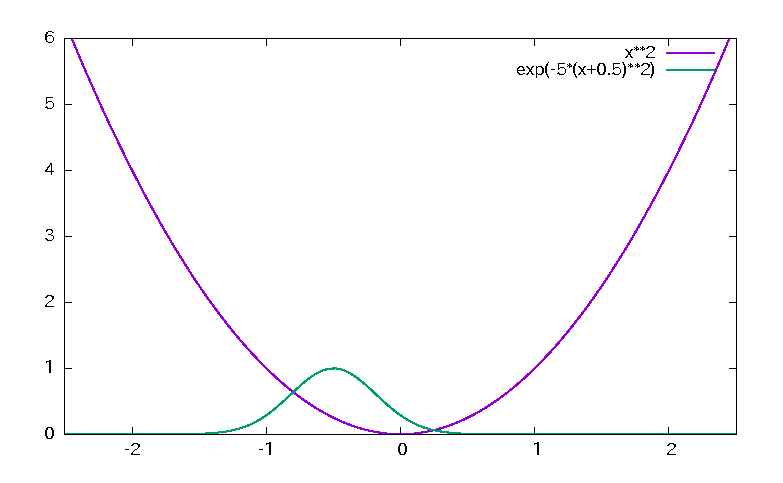
\includegraphics[width = 7cm]{./wave_packet.eps}
  \label{fig1}
\end{figure}
\\
この波束が調和型トラップによって振動する. 古典粒子が調和振動子トラップ内で振動するとき, 位相空間上の点は楕円を描くように動くはずでありWigner関数も同様の動きをするが, 相空間上では$q, p$方向の広がりがある. 
\begin{figure}[htbp]
  \begin{center}
    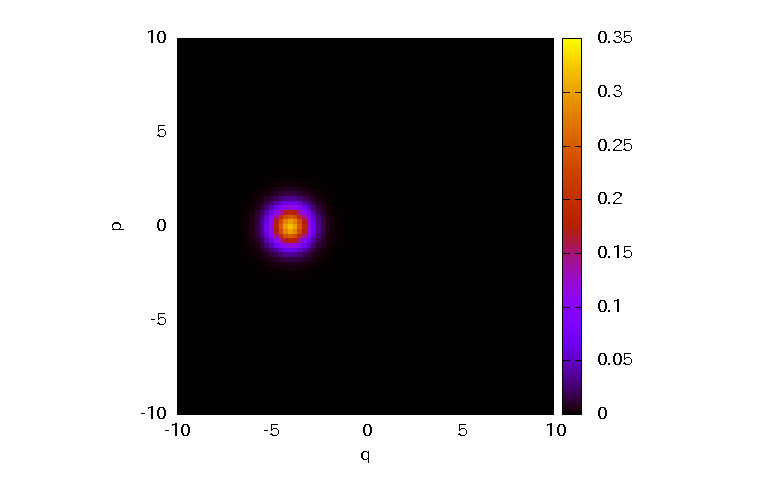
\includegraphics[width = 12cm]{./wigner_function.eps}
  \end{center}
  \label{fig2}
\end{figure}\\
こんなほんやりした玉みたいなのが位相空間上をぐるぐる回るはず. 
\newpage
\chapter{経路積分}
\section{量子力学の復習}
\subsection{自由粒子}
自由粒子を記述するSchr\"odinger方程式は
\begin{eqnarray}
  i\partial_t\ket{\psi(t)} = \frac{\hat{p}^2}{2m}\ket{\psi(t)}
\end{eqnarray}
これを$p$-表示に移すと簡単に解ける:
\begin{eqnarray}
  i\partial_t\bra{p}\ket{\psi(t)} &=& \bra{p}\frac{\hat{p}^2}{2m}\ket{\psi(t)} = \frac{p^2}{2m}\bra{p}\ket{\psi(t)}\\
  \therefore \bra{p}\ket{\psi(t)} &=& Ce^{-i\frac{\hat{p}^2}{2m}t}
\end{eqnarray}
これを運動量固有値$p$でパラメトライズされたケットで表現すると
\begin{eqnarray}
  \ket{p, t}_S = \ket{p}e^{-i\frac{\hat{p}^2}{2m}t}
\end{eqnarray}
ということ.もちろん$_S\bra{p', t}\ket{p, t}_S = \delta(p-p')$. 一般解はこの線型結合で書ける:
\begin{eqnarray}
  \ket{\Psi, t} = \int dp f(p)\ket{p}e^{-i\frac{\hat{p}^2}{2m}t}
\end{eqnarray}
これは規格化条件$\bra{\Psi, t}\ket{\Psi, t} = 1$を満たしているものとする. ここで, $t = 0$で$x = 0$に局在している波束を用意する:
\begin{eqnarray}
  \bra{x}\ket{\psi} = \frac{1}{(\pi\alpha)^{\frac{1}{4}}}e^{-\frac{1}{2\alpha}x^2}\label{FreeWavePacket}
\end{eqnarray}
これの$p$-表示は完全系を挿入することで求まる:
\begin{eqnarray}
  \bra{p}\ket{\psi} = \int dx\bra{p}\ket{x}\bra{x}\ket{\psi} = \qty(\frac{\alpha}{\pi})^{\frac{1}{4}}e^{-\frac{\alpha}{2}p^2}
\end{eqnarray}
\\

\fbox{問1} $\bra{x}\ket{p} = \frac{1}{\sqrt{2\pi}}e^{ipx}$であることを示せ. また, この操作がFourier変換と等価であることを確認せよ.\\

ここで$\Delta t$だけ時間発展させると
\begin{eqnarray}
  \bra{p}e^{-iH\Delta t}\ket{\psi} = \qty(\frac{\alpha}{\pi})^{\frac{1}{4}}e^{-\frac{\alpha}{2}p^2}e^{-i\frac{\hat{p}^2}{2m}\Delta t}
\end{eqnarray}
である. \\

\fbox{問2} $i\partial_t\ket{\psi} = \hat{H}\ket{\psi}$の形式解が$e^{-i\hat{H}t}\ket{\psi}$であることを確かめよ.\\

これを$x$-表示に移すと
\begin{eqnarray}
  \bra{x}\ket{\psi} = \qty(\frac{\alpha}{\pi})^{\frac{1}{4}}\sqrt{\frac{1}{\alpha + i\frac{\Delta t}{m}}}e^{-\frac{1}{\alpha + i\frac{\Delta t}{m}}x^2}\label{DevelopedFreeWavePacket}
\end{eqnarray}
となる. 自由粒子の波束の幅は時間発展と共に広がっていくことがわかる.
\subsection{Green関数}
以上のような「様々な初期波束を置いてみて, 時間発展に従って波動関数がどのように変化するのか」を考える問題ではGreen関数(伝搬関数, propagator)を計算しておくと便利.
\begin{eqnarray}
  \bra{x}\ket{\psi(t)} = \bra{x}e^{-iH(t-t_0)}\ket{\psi(t_0)} &=& \int dx'\bra{x}e^{-iH(t-t_0)}\ket{x'}\bra{x'}\ket{\psi(t_0)}\\
  &=& \int dx' G(x, t;x', t_0)\bra{x'}\ket{\psi(t_0)}
\end{eqnarray}
Green関数$G(x, t;x', t_0)$は, 時刻 $t_0$ に場所 $x_0$ にいた粒子が時刻$t$ に場所 $x$ に移動している確率振幅密度のようなもの. このGreen関数が分かりさえすれば波束を掛けて積分することで時間発展を追うことができる. このGreen関数を計算する方法としてよく用いられるのが経路積分である.

Green関数の数学的な定義などについては別途勉強しましょう.
\section{経路積分の基礎}
\subsection{経路積分の導出}
伝搬関数は初期状態を$(q_i, t_i)$, 終状態を$(q_f, t_f)$とすると
\begin{eqnarray}
  K(q_f, t_f;q_i, t_i) \equiv \bra{q_f, t_f}e^{-i\hat{H}(t_f-t_i)}\ket{q_i, t_i}
\end{eqnarray}
と定義できる\footnote{以降伝搬関数は$K$と書く. これをFeynman核(Feynman kernel)と呼ぶ. $t>0$を約束すればGreen関数とFeynman核は同じもの. }. $\ket{q, t}$は時刻$t$で粒子が座標$q$に局在している$\hat{q}$の固有状態である. 自由粒子などの簡単なモデルであれば伝搬関数の計算もそんなに大変ではないが, もっと複雑なモデルではそう簡単に求まらない. これをうまく計算するために経路積分(Path Integral)を導出する.

まず時間を微小区間$\delta t$に分割する:
\begin{eqnarray}
  e^{-i\hat{H}(t_f-t_i)} = \prod_{I=1}^Ne^{-i\hat{H}\delta t},\hspace{0.5cm} \delta t = \frac{t_f - t_i}{N}
\end{eqnarray}
時間を$N+1$分割したことになる. $\hat{q}$が$\hat{p}$より右側にあることを仮定し, 各分割点に位置演算子$\hat{q}(t_i + I\delta t)$の固有状態$\ket{q_I}$の完全系
\begin{eqnarray}
  \int dq_I \ket{q_I}\bra{q_I} = 1
\end{eqnarray}
を挟むと伝搬関数は以下のように書き直せる:
\begin{eqnarray}
\nonumber  K(q_f, t_f;q_i, t_i) =\int dq_{N-1}dq_{N-2}\cdots dq_{I}\cdots dq_2dq_1\bra{q_f}e^{-i\hat{H}\delta t}\ket{q_{N-1}}\bra{q_{N-1}}e^{-i\hat{H}\delta t}\ket{q_{N-2}}\bra{q_{N-2}}\cdots\\
  \cdots\bra{q_{I+1}}e^{-i\hat{H}\delta t}\ket{q_{I}}\cdots\bra{q_2}e^{-i\hat{H}\delta t}\ket{q_1}\bra{q_1}e^{-i\hat{H}\delta t}\ket{q_i}
\end{eqnarray}
以下では$\bra{q_{I+1}}e^{-i\hat{H}\delta t}\ket{q_{I}}$を計算することを考える. これに運動量演算子$\hat{p}(t_i + I\delta t)$の固有状態$\ket{p_I}$の完全系
\begin{eqnarray}
  \int dp_I \ket{p_I}\bra{p_I} = 1
\end{eqnarray}
を挿入する:
\begin{eqnarray}
  \bra{q_{I+1}}e^{-i\hat{H}\delta t}\ket{q_{I}} &=& \int dp_I\bra{q_{I+1}}\ket{p_I}\bra{p_I}e^{-i\hat{H}\delta t}\ket{q_{I}}\\
  &=&\int dp_I\bra{q_{I+1}}\ket{p_I}e^{-iH(q_I, p_I)\delta t}\bra{p_I}\ket{q_{I}}
\end{eqnarray}\\

\fbox{問3} $\hat{H}$に演算子$\hat{q}, \hat{p}$が含まれていることから, $\bra{p_I}e^{-i\hat{H}\delta t}\ket{q_{I}}$のハットハミルトニアンが$c$-数の$H(q_I, p_I)$に化けることを示せ.\\

$\bra{q}\ket{p}$は平面波になることから
\begin{eqnarray}
  \bra{q_{I+1}}e^{-i\hat{H}\delta t}\ket{q_{I}} &=& \frac{1}{2\pi}\int dp_Ie^{i\qty(p_I\frac{q_{I+1}-q_I}{\delta t}-iH(q_I, p_I)){\delta t}}
\end{eqnarray}
$\delta t \rightarrow 0$の極限では$\cfrac{q_{I+1}-q_I}{\delta t}\rightarrow \cfrac{dq}{dt}$であることから
\begin{eqnarray}
  K(q_f, t_f;q_i, t_i) &=& \int {\cal D}p{\cal D}qe^{i\int_{t_i}^{t_f}dt\qty(p\frac{dq}{dt} - H)}\\
  {\cal D}p{\cal D}q &=& \prod_{I=0}^{N}\frac{{\cal D}p{\cal D}q}{2\pi}
\end{eqnarray}\\

\fbox{問4} expの肩が(和ではなく)積分になることを確認せよ.\\

$N$はいずれ$\infty$になるので, 無限回の積分を行わなくてはいけない。この積分は $q(t_i) = q_i, q(t_f) = q_f$ となるような境界条件をつけて行うとする.

$H = \frac{p^2}{2m} + V(q)$の場合について考える:
\begin{eqnarray}
  K(q_f, t_f;q_i, t_i) &=& \int {\cal D}p{\cal D}qe^{i\int_{t_i}^{t_f}dt\qty(p\frac{dq}{dt} - \frac{p^2}{2m} - V(q))} = \int {\cal D}p{\cal D}qe^{i\int_{t_i}^{t_f}dt\qty(-\frac{(p-m\dot{q})^2}{2m} + \frac{\dot{q}^2}{2m} - V(q))}
\end{eqnarray}
これで$p$について積分が可能. $q$の積分は$V(q)$の具体系が与えられて初めて計算が可能になる. $p$の積分を実行し, その解が${\cal N}$だったとすると
\begin{eqnarray}
  K(q_f, t_f;q_i, t_i) = {\cal N}\int {\cal D}qe^{i\int_{t_i}^{t_f}dt\qty(\frac{\dot{q}^2}{2m} - V(q))}\label{FeynmanPropagator}
\end{eqnarray}
$\exp$の肩に作用(action)$S[q(t)] = \int_{t_i}^{t_f}dt\qty(\frac{\dot{q}^2}{2m} - V(q))$に虚数単位を掛けて積分すれば伝搬関数が求まることがわかる. これが経路積分である.

作用が(プランク定数より)十分大きい場合$\exp(iS)$は極値の近傍を除いて激しく振動して積分に効いてこないことが期待される. この極値のみを取り出してきたものを「古典極限」と呼ぶ. 作用がプランク定数と同程度のオーダーを持つ場合, 極値近傍以外にも積分に効いてくる可能性があり, これが量子効果として取り入れられることになる.\\

\fbox{問5} 無次元化をしない場合, 経路積分の被積分関数は$\exp\qty(iS/\hbar)$と書ける. $S$がプランク定数$\hbar$より十分大きい時, $S$の極値以外の積分が値に効いてこない理由を考えよ. 

\subsection{自由粒子 : 経路積分を使わない方法}
自由粒子($V(q) = 0$)の場合は経路積分を使わなくても伝搬関数がすぐに求まる. まず$p$-表示で確率振幅を書き下す:
\begin{eqnarray}
  \bra{p_f}e^{-i\frac{\hat{p}^2}{2m}(t_f - t_i)}\ket{p_i} = e^{-i\frac{p_f^2}{2m}(t_f - t_i)}\delta(p_f - p_i)
\end{eqnarray}
これを$x$-表示に移す:
\begin{eqnarray}
 K(x_f, t_f;x_i, t_i) = \bra{x_f}e^{-i\frac{\hat{p}^2}{2m}(t_f - t_i)}\ket{x_i} &=& \int dp\bra{x_f}\ket{p}\bra{p}e^{-i\frac{\hat{p}^2}{2m}(t_f - t_i)}\ket{x_i}\\
  &=&\sqrt{\frac{m}{2\pi i(t_f-t_i)}}e^{-i\frac{m}{2(t_f - t_i)}(x_f - x_i)^2}\label{FreePropagator}
\end{eqnarray}\\
\fbox{問6} (\ref{FreePropagator})(\ref{DevelopedFreeWavePacket})を用いて(\ref{FreeWavePacket})を再現せよ.

\subsection{自由粒子 : 経路積分の方法}
まずは伝搬関数(の被積分関数)を時間について離散化する($\dot{x} = \cfrac{x_{j+1} - x_j}{\delta t}$):
\begin{eqnarray}
e^{-i\int dt\frac{m\dot(x)^2}{2}} \rightarrow \prod_{j=0}^Ne^{\frac{im}{2}\qty(\frac{x_{j+1} - x_j}{\delta t})\delta t}
\end{eqnarray}
ただし$x_0 = x_i, x_{N+1} = x_f$とする. これに$\int dx_1dx_2\cdots dx_N$をかけて積分すれば(\ref{FeynmanPropagator})が計算できたことになる. ここで公式
\begin{eqnarray}
  \int_{-\infty}^{\infty} dx e^{ia(x-x_1)^2 + ib(x-x_2)^2} = \sqrt{\frac{i\pi}{a+b}}e^{i\frac{ab}{a+b}(x_1-x_2)^2}\label{Gauss}
\end{eqnarray}
を用いる. \\

\fbox{問7} (\ref{Gauss})を証明せよ.\\

$x_1$に関する積分:
\begin{eqnarray}
  \int dx_1 e^{i\frac{m}{2\delta t}\qty((x_i - x_1)^2-(x_1 - x_2)^2)} = \sqrt{\frac{i\pi\delta t}{m}}e^{-i\frac{m}{4\delta t}(x_i - x_2)^2}
\end{eqnarray}
これより, $x_2$の積分は:
\begin{eqnarray}
  \int dx_2 e^{i\frac{m}{2\delta t}\qty(\frac{1}{2}(x_i - x_2)^2-(x_2 - x_3)^2)} = \sqrt{\frac{4i\pi\delta t}{3m}}e^{-i\frac{m}{6\delta t}(x_i - x_3)^2}
\end{eqnarray}
これを繰り返していくと$x_n$の積分因子として$\sqrt{\cfrac{i2n\pi\delta t}{(n+1)m}}$が現れることがわかる. 全積分が終わったとき
\begin{eqnarray}
  K(x_f, t_f;x_i, t_i) = \bra{x_f}e^{-i\frac{\hat{p}^2}{2m}(t_f - t_i)}\ket{x_i} = {\cal N}\qty(\sqrt{\frac{i2\pi\delta t}{m}})^N\sqrt{\frac{1}{N+1}}e^{i\frac{m}{2(N+1)\delta t}(x_f - x_i)^2}\label{Kernel}
\end{eqnarray}
${\cal N}$は$p$積分の結果出てくる因子で, 積分1回につき$\sqrt{\cfrac{m}{2\pi i\delta t}}$が出てくる. さらに$\delta t(N+1) = t_f - t_i$であることを用いると
\begin{eqnarray}
  K(x_f, t_f;x_i, t_i ) &=&\sqrt{\frac{m}{2\pi i(t_f-t_i)}}e^{-i\frac{m}{2(t_f - t_i)}(x_f - x_i)^2}
\end{eqnarray}
となり, (\ref{FreePropagator})と一致している.\\

\fbox{問8} $p$成分の積分を計算せよ.\\

\fbox{問9} 数学的帰納法を用いてFeynman kernelが(\ref{Kernel})のように計算できることを示せ.\\

経路積分を使わない方法に比べてかなり面倒ですが, モデルがもっと複雑になると有り難みが出てきます. 
\section{数値計算の準備及び経路積分のイメージ}
直感的理解へ向けて経路積分について数値計算を行う.
\subsection{基底波動関数と伝搬関数}
伝搬関数を束縛状態の固有関数$\ket{n}$で展開:
\begin{eqnarray}
  G(x, t; x_0, t_0=0) \equiv \bra{x}e^{-i\hat{H}(t-t_0)}\ket{x_0} = \sum_n\bra{x}\ket{n}\bra{n}e^{-i\hat{H}t}\ket{x_0} = \sum_n\psi_n(x)\psi_n^*(x_0)e^{-iE_nt}
\end{eqnarray}
ここで$t = -i\tau$として$\tau\rightarrow\infty$を考えると, 高い励起状態は指数関数的に減衰していくことがわかる. これより伝搬関数と基底波動関数の関係
\begin{eqnarray}
  &&G(x, t= 0 -i\tau; x_0, t_0=0) \rightarrow \psi_0(x)\psi_0^*(x_0)e^{E_0\tau}\\
  &\therefore&|\psi_0(x)|^2 \rightarrow e^{-E_0\tau}G(x, t= 0 -i\tau; x_0=x, t_0=0)\label{GroundGreen}
\end{eqnarray}
が明らかになる. 第二式は始点と終点が同じになっていることに注意. Green関数から基底波動関数の情報を抜き出すためには, 虚時間を導入し時間発展を行えば良い. これを虚時間発展法と呼ぶ.
\subsection{作用とラグランジアン}
ラグランジアンを虚時間で記述すると, ハミルトニアンに化ける:
\begin{eqnarray}
  &&L\qty(x, \frac{dx}{dt}) = \frac{m}{2}\qty(\frac{dx}{dt})^2 - V(x)\\
  &\rightarrow& L\qty(x, \frac{dx}{-id\tau}) = -\frac{m}{2}\qty(\frac{dx}{d\tau})^2 - V(x) = -H\qty(x, \frac{dx}{d\tau})
\end{eqnarray}
これにより作用がラグランジアンの積分からハミルトニアンの積分に書き換えられる:
\begin{eqnarray}
  S[x(t)] &=& \int_{t_0=0}^{t}dtL(x, t) = i\int_{\tau_0=0}^{\tau}d\tau H(x,\tau)\label{prob10_1}\\
  G(x, -i\tau; x_0, 0) &=& \qty(\frac{1}{2\pi})^{N+1}\int dx_1 dx_2\cdots dx_N e^{-\int_0^{\tau} H(\tau)}\label{prob10_2}
\end{eqnarray}\\

\fbox{問10} (\ref{prob10_1})(\ref{prob10_2})を確かめよ. \\

\subsection{作用積分の簡略化}
前述のハミルトニアンの積分を差分化で書き直し, 数値計算に持ち込めるようにする:
\begin{eqnarray}
  \int H(\tau) &\simeq& \sum_j\epsilon E_j = \epsilon W(\{x_j\})\\
  W(\{x_j\}) &\equiv& \sum_j\qty[\frac{m}{2}\qty(\frac{x_{j} - x_{j-1}}{\epsilon})^2 + V\qty(\frac{x_{j} + x_{j-1}}{2})]
\end{eqnarray}
規格化を考慮したうえで(\ref{GroundGreen})に代入する:
\begin{eqnarray}
  |\psi_0(x)|^2 &=& \lim_{\tau\rightarrow\infty}\frac{G(x, t=-i\tau;x_0=x, t_0=0)}{\int dx G(x, t=-i\tau;x_0=x, t_0=0)}\\
  &=&\frac{1}{Z}\lim_{\tau\rightarrow\infty}\int dx_1 dx_2\cdots dx_N e^{-\epsilon W(x, x_1,..., x_N)}\label{PsiW}\\
  Z &=& \lim_{\tau\rightarrow\infty}\int dx dx_1 dx_2\cdots dx_N e^{-\epsilon W}
\end{eqnarray}
$W$はエネルギー線績分になっている. また$W(x, x_1,..., x_N)$は始点と終点を$x$に固定している.
\subsection{経路とは}
(\ref{prob10_2})の$\exp$の肩においてハミルトニアンを時間軸に沿って積分している. また$S[x(t)] = i\int_{\tau_0=0}^{\tau}d\tau H(x, \tau)$から作用は$x(t)$の経路によって決定される. つまり, 「取りうるすべての$x(t)$の経路についてエネルギー(ハミルトニアン)を足しあげていく」ことが経路積分の具体的なイメージである. エネルギーが大きい経路が効いてこない理由は(\ref{prob10_2})から直感的にわかる. 
\subsection{経路の取り方}
$|\psi_0(x)|^2$を求めたい訳だが, 数値計算の上では離散化するので$|\psi_0(x[1])|^2, |\psi_0(x[2])|^2, |\psi_0(x[3])|^2 ... |\psi_0(x[N-1])|^2$を求めることになる. 本来なら$G(x[1], -i\tau; x[1], 0), G(x[2], -i\tau; x[2], 0), G(x[3], -i\tau; x[3], 0), ... G(x[N-1], -i\tau; x[N-1], 0)$について別々の初期設定で計算する必要がある.これを別々に計算すると計算コストが非常に高くなる.$x_j$は時間で差分化, $x[j]$は空間で差分化していることに注意.

具体的な計算においては(\ref{PsiW})を各$x[1],x[2] ...$について計算すればよいのだが
\begin{eqnarray}
  |\psi_0(x[1])|^2 &=&\frac{1}{Z}\lim_{\tau\rightarrow\infty}\int dx_1 dx_2\cdots dx_N e^{-\epsilon W(x[1], x_1, x_2, ...)}\\
  |\psi_0(x[2])|^2 &=&\frac{1}{Z}\lim_{\tau\rightarrow\infty}\int dx_1 dx_2\cdots dx_N e^{-\epsilon W(x[2], x_1, x_2, ...)}\\
  \nonumber  &&\vdots
\end{eqnarray}
における$W(x[1], x_1, x_2, ...)$と$W(x[2], x_1, x_2, ...)$は始点(終点)が異なるので, それぞれ別々に計算を実行しなければならない. これが計算コストの肥大化の原因である.
\subsection{処方箋}
この問題に関する処方箋はRubinの本\footnote{Rubin H. Landau, {\it Computational Physics} (1997) pp. 313-317}にあるのでこれを参考勉強するのがいいと思います. が, 翻訳があまり良くないのかそもそも原文の内容が丁寧でないためか, 理解するのはなかなか難しいと思います. 理解のための重要なポイントは
\begin{itemize}
\item[1.] $x_0$が始点(終点)の経路における$x_i$を$x'_i$にフリップしたときに$x_0$からの作用積分が $x_i$からの作用積分と同じ値であることを利用して$|\psi(x'_i)|^2$を求めることが経路積分の計算と等価であること
\item[2.] 作用を計算して確率分布に計上することと, フリップする確率をBoltzmann分布で与えてその経路(格子点)に乗った粒子をそのまま足し上げることがだいたい等価であること
\end{itemize}
の2点にあると思います. この2つがMonte Carlo法・Metropolis法による数値計算を正当化しています.

是非一緒にお勉強しましょう. 
%% \subsection{計算のテクニック}
%% この問題を解消するために(\ref{PsiW})を以下のように変形する:
%% \begin{eqnarray}
%%   |\psi_0(x)|^2  &=&\frac{1}{Z}\lim_{\tau\rightarrow\infty}\int dx_0 dx_1 dx_2\cdots dx_N \delta(x - x_0)e^{-\epsilon W(x_0, x_1,..., x_N)}
%% \end{eqnarray}
%% これで始点(終点)を$x_0$に固定したことになる. 例えば$\psi(x[1]), \psi(x[2]), \psi(x[3])\cdots$を計算したければ
%% \begin{eqnarray}
%%   |\psi_0(x[1])|^2  &=&\frac{1}{Z}\lim_{\tau\rightarrow\infty}\int dx_0 dx_1 dx_2\cdots dx_N \delta(x[1] - x_0)e^{-\epsilon W(x_0, x_1,..., x_N)}\\
%%   |\psi_0(x[2])|^2  &=&\frac{1}{Z}\lim_{\tau\rightarrow\infty}\int dx_0 dx_1 dx_2\cdots dx_N \delta(x[2] - x_0)e^{-\epsilon W(x_0, x_1,..., x_N)}\\
%%   |\psi_0(x[3])|^2  &=&\frac{1}{Z}\lim_{\tau\rightarrow\infty}\int dx_0 dx_1 dx_2\cdots dx_N \delta(x[3] - x_0)e^{-\epsilon W(x_0, x_1,..., x_N)}\\
%% \nonumber  &&\vdots
%% \end{eqnarray}
%% を計算すればよい. ここで重要なのは「被積分関数はデルタ関数を除いてどれも同じ」ことである.つまり, $x_0$を始点に置いたすべての$(x_0, x_1, ..., x_N)$についてエネルギー線績分を計算した後に$x[1], x[2], x[3], ...$のそれぞれについてのみ値をピックアップすればよい.
%% \subsubsection{いやだから...}
%% 結局デルタ関数で$x_0$が$x[1]$やら$x[2]$やらに変えられるわけだから, やはり別々に$W(x[1], x_1, x_2, ...)$と$W(x[2], x_1, x_2, ...)$を計算しなければならないのでは?と思うでしょう.

%% この問題を巧く解決する方法があります\footnote{Rubin H. Landau, {\it Computational Physics} (1997) pp. 313-317}.

\newpage
\chapter{Ising模型}
\section{Ising模型と熱統計力学の基礎}
強磁性体を記述するモデルのひとつ.
\subsection{ハミルトニアン}
ハミルトニアンを
\begin{eqnarray}
  H = -J\sum_{\ev{i, j}}s_i\cdot s_j
\end{eqnarray}
とする. $\ev{i, j}$は隣接サイト間のみの和を表す. $J$は相互作用定数. $s$はスピン. スピンはアップ($s = 1$)とダウン($s = -1$)の2種類. 非常に単純なスピン系モデルでありながら相転移の記述が可能である. 1・2次元系については厳密解が求められている.

外部磁場を考慮したモデルもある:
\begin{eqnarray}
  H = -J\sum_{\ev{i, j}}s_i\cdot s_j -h\sum_i s_i\label{Ising2}
\end{eqnarray}

\subsection{平衡状態}
系の平衡状態はHelmholtzエネルギー
\begin{eqnarray}
  F = U -TS
\end{eqnarray}
が最小になるように決まる. 低温 ($T \ll U/S$)ならば内部エネルギー $U = \ev{H}$ がleading であり, これを最小化するようにスピンの向きが揃う. これを強磁性体と呼ぶ. 一方で高温ならばエントロピーの項が優勢なのでエントロピーが最大になるようにスピンの向きがバラバラになる. これを常磁性体と呼ぶ.

\subsection{相転移}
Gibbs自由エネルギーの1回微分が不連続変化をするときこれを第一種相転移と呼び, Gibbs自由エネルギーの2回微分については第二種相転移と呼ぶ. 第一種は体積, エントロピーとか. 
\begin{eqnarray}
  \qty(\frac{\partial G}{\partial p})_T = V, \hspace{1cm} \qty(\frac{\partial G}{\partial T})_p = -S
\end{eqnarray}
第二種は比熱など.
\begin{eqnarray}
\frac{\partial^2 G}{\partial T^2} = -\frac{\partial S}{\partial T} = -\frac{C_P}{T}
\end{eqnarray}
有限温度1次元Ising模型は相転移を起こさないが, 2次元系はその限りではない.

\section{Ising模型の厳密解}
\subsection{1次元Ising模型 : 平均場近似}
まずは厳密解の前にIsing模型を平均場近似で解析してみる. 多体系で相互作用を平均場として理解することは非常に重要なので, 手法として知っておく必要がある.

平均場近似ではまず任意のサイトのスピンに着目し, その周囲のスピンからの影響を時間や空間によらない平均値で置き換える. スピンを
\begin{eqnarray}
  s_i = \ev{s} + \delta s_i
\end{eqnarray}
置くことにする. これを(\ref{Ising2})に代入:
\begin{eqnarray}
  H &=& -H_{\rm{eff}}\sum_{i=1}^N s_i + \frac{NzJ\ev{s}^2}{2}\\
  H_{\rm{eff}} &=&  h + zJ\ev{s}
\end{eqnarray}
ここで$\delta s$の2次は無視している. $N$はスピンの総数, $z$は最隣接サイト数(1次元なら2, 2次元なら4)である. 計算途中で
\begin{eqnarray}
  \sum_{\ev{i, j}}s_i = z\sum_i s_i, \hspace{0.5cm}\sum_{\ev{i, j}}1 = \frac{1}{2}zN
\end{eqnarray}
を用いている. これより分配関数は
\begin{eqnarray}
  Z &=& \exp\qty(-\beta H) = \exp\qty[-\beta\qty(-H_{\rm{eff}}\sum_{i=1}^N s_i + \frac{NzJ\ev{s}^2}{2})] = Z_0\qty(\prod_iZ_i) = Z_0(Z_i)^N\\
  Z_0 &=& \exp\qty(-\beta\frac{NzJ\ev{s}^2}{2}), \hspace{0.5cm}Z_i = \sum_{s_i = 1, -1}e^{\beta H_{\rm{eff}}s_i} = 2\cosh\qty(\beta H_{\rm{eff}})
\end{eqnarray}
全体の分配関数は
\begin{eqnarray}
  Z = \exp\qty(-\beta\frac{NzJ\ev{s}^2}{2})2^N\cosh^N\qty(\beta H_{\rm eff})
\end{eqnarray}
Helmholtzエネルギーは
\begin{eqnarray}
  F = \frac{NzJ}{2}\ev{s}^2 - Nk_BT\log\qty[2\cosh\qty(\beta H_{\rm eff})]
\end{eqnarray}
磁化は単位体積あたりのスピン数を$n$としたときに$M=n\ev{s}$であるが, 今回すべてのスピンは等価と考えているので$\ev{s_i}$を計算すれば十分である:
\begin{eqnarray}
  \ev{s_i} &=& \frac{1}{Z}\sum_{s_i}\cdots\sum_{s_i}\cdots s_ie^{-\beta H} = \frac{1}{Z_i}\sum_{s_i = -1, 1}s_ie^{\beta s_iH_{\rm eff}}\\
  &=& \tanh\qty(\beta H_{\rm eff})
\end{eqnarray}
これは自己無同着方程式である.
\subsection{1次元Ising模型 : 厳密解}
教科書を参考にしながら是非自分で手を動かして解いてみてください.
\subsection{2次元Ising模型}
2次元Ising模型の厳密解はOnsagerによって求められている:
\begin{eqnarray}
  \frac{U}{N} &=& -J\coth{2\beta J}\qty[1+\frac{2}{\pi}\kappa_1 K(\kappa)]\\
  \frac{C_H}{N} &=& k_B(\beta J\coth{2\beta J})^2\frac{2}{\pi}\qty[2K(\kappa)-2E(\kappa) - (1-\kappa_1)\qty(\frac{2}{\pi} + \kappa_1K(\kappa))]
\end{eqnarray}
$K(\kappa), E(\kappa)$は楕円積分:
\begin{eqnarray}
  K(\kappa) = \int_0^{\frac{\pi}{2}}\frac{d\theta}{\sqrt{1-\kappa^2\sin^2{\theta}}}\\
  E(\kappa) = \int_0^{\frac{\pi}{2}}d\theta \sqrt{1-\kappa^2\sin^2{\theta}}
\end{eqnarray}
導出は難しいので, これが数値計算と一致するかどうかを確かめたい. 
  
\section{数値計算}
\subsection{Monte Carlo法}
系はHelmholtzエネルギーを最小にするように平衡状態を決める(ゼロ温度の場合は内部エネルギーが最小).これを実現するためには, 任意のサイトの状態を変化させて内部エネルギーが小さくなるようにする操作を繰り返せば良い. 「任意のサイトを選ぶ」ために乱数を用いることになるが, 乱数を用いるアルゴリズムの総称がMonte Carlo法である.

単純に前述の通り内部エネルギーが最小な平衡状態はゼロ温度なので, 有限温度系に拡張するためには工夫が必要である. 
\subsection{Metropolis法}
系が平衡状態にあるとき, 内部エネルギーの分布を$P(E)$, エネルギー$E' \rightarrow E$遷移確率を$W(E, E')$とすると
\begin{eqnarray}
  W(E, E')P(E') = W(E', E)P(E)\label{equiliblium}
\end{eqnarray}
が成立している. $P(E')$の状態が$P(E)$の状態に遷移しようとする流れとその逆の流れが平衡状態にあるということである. 系のエネルギー分布がカノニカル分布になることを仮定すると, 
\begin{eqnarray}
  P(E) = \frac{e^{-\beta E}}{Z(\beta)}
\end{eqnarray}
であることがわかる. $Z(\beta)$は分配関数. これを(\ref{equiliblium})に代入すると以下の関係式を得る:
\begin{eqnarray}
  e^{-\beta(E-E')} = \frac{W(E, E')}{W(E', E)}\label{equiliblium2}
\end{eqnarray}
ここで, (\ref{equiliblium2})を満たすような$W(E, E')$を与える: 
\begin{eqnarray}
  W(E, E') =
  \begin{cases}
    1 & (E \leq E')\\
    e^{-\beta(E-E')} & (E > E')
  \end{cases}
\end{eqnarray}
これがMetropolis法である.

Isingモデルに置き換えると, スピンをフリップしたときにエネルギー的に安定ならばそのままにして, 不安定な場合も, ボルツマン因子に依る確率でフリップを許可する. これで有限温度系への拡張が可能になる. 
\newpage
\subsection{2次元Ising模型}
シミュレーション結果:
\begin{figure}[htbp]
  \begin{center}
    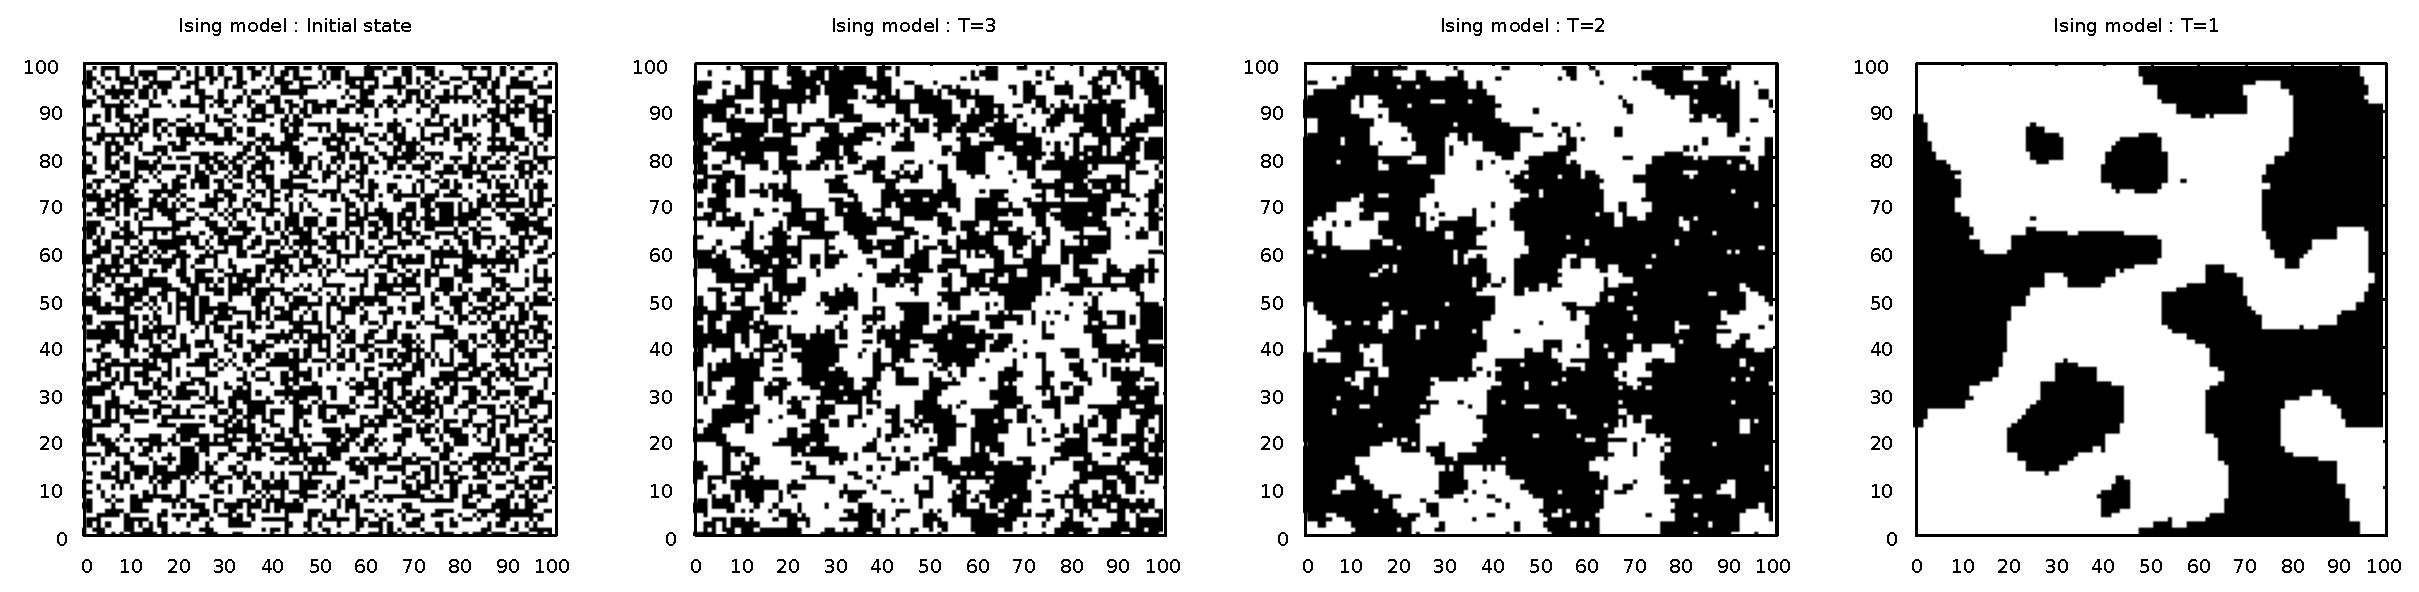
\includegraphics[width = 17cm]{./spin.eps}
  \end{center}
  \label{fig1}
\end{figure}\\
\begin{figure}[htbp]
  \begin{center}
    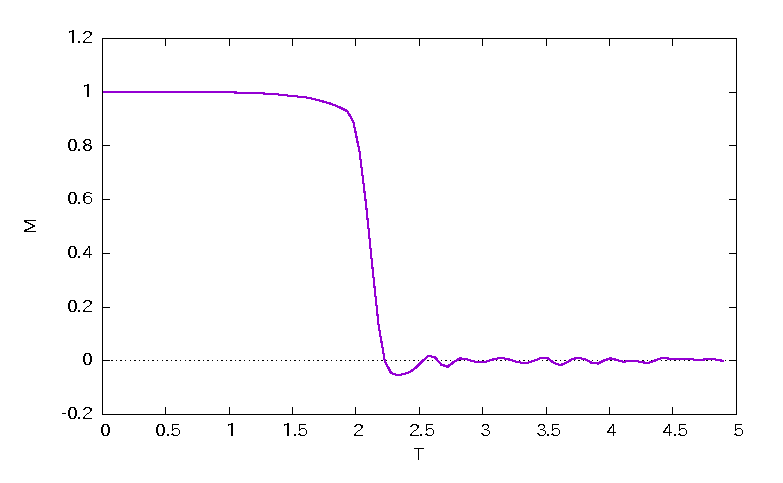
\includegraphics[width = 10cm]{./magnetization.eps}
  \end{center}
  \label{fig2}
\end{figure}\\
\begin{figure}[htbp]
  \begin{center}
    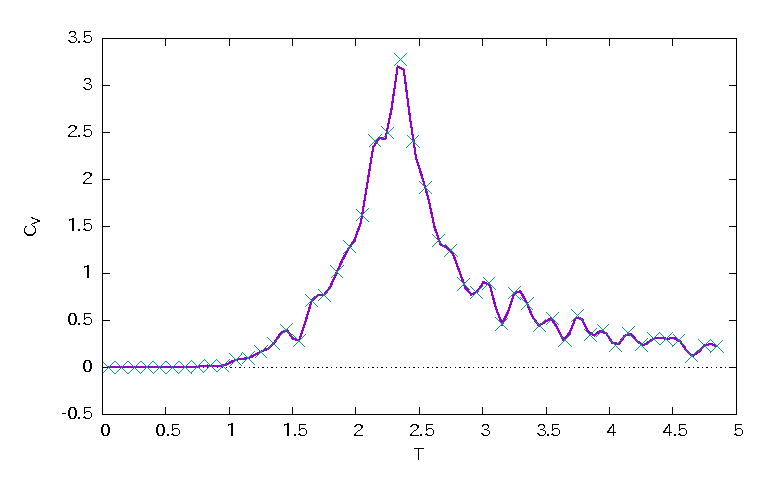
\includegraphics[width = 10cm]{./specificheat.eps}
  \end{center}
  \label{fig2}
\end{figure}\\

磁区の図は$N=100^2, J=1$, 磁化と比熱は$N=16^2, J=1$で計算した. 以上の図から
\begin{itemize}
\item 温度が下がるほどはっきりとした磁区が形成されること
\item 磁化・比熱は転移温度($T_C \simeq 2.26$)付近でdrasticに変化していること
\item 2次相転移が起こっている(であろう)こと
\end{itemize}
などがわかる.

\subsection{数値計算上の注意}
\subsubsection{乱数}
なるべく良い乱数を用いるようにしましょう. C言語のrand()はあまり良くありません. 単純な線形合同法では周期が短く大量の乱数を用いるシミュレーションには向きません. Mersenne twisterなどのアルゴリズムを用いましょう.
\subsubsection{ローカルな極小点}
ゼロ温度系ではあまり明確な磁区が生まれません. ただのMonte Carlo法ではローカルな極小点にハマるとそこから抜け出せないからです. Metropolis法を適応するとある程度解決しますが, やはり正の磁区と負の磁区に分かれるのでグローバルな磁化は熱力学極限とは異なる値を示します. 上の図の$T=1$もやはりローカルな極小点であり真の最小点であるスピンが全て揃った状態にはなりません. これを解決するために, 物理量の計算の際は$T=0$でスピンが全て揃った状態を用意しそこからMonte Carloシミュレーションを行っています. 焼きなまし法を用いるとどんな初期状態でもHelmholtzエネルギーが最小な状態を作れるかもしれません.
\begin{figure}[htbp]
  \begin{center}
    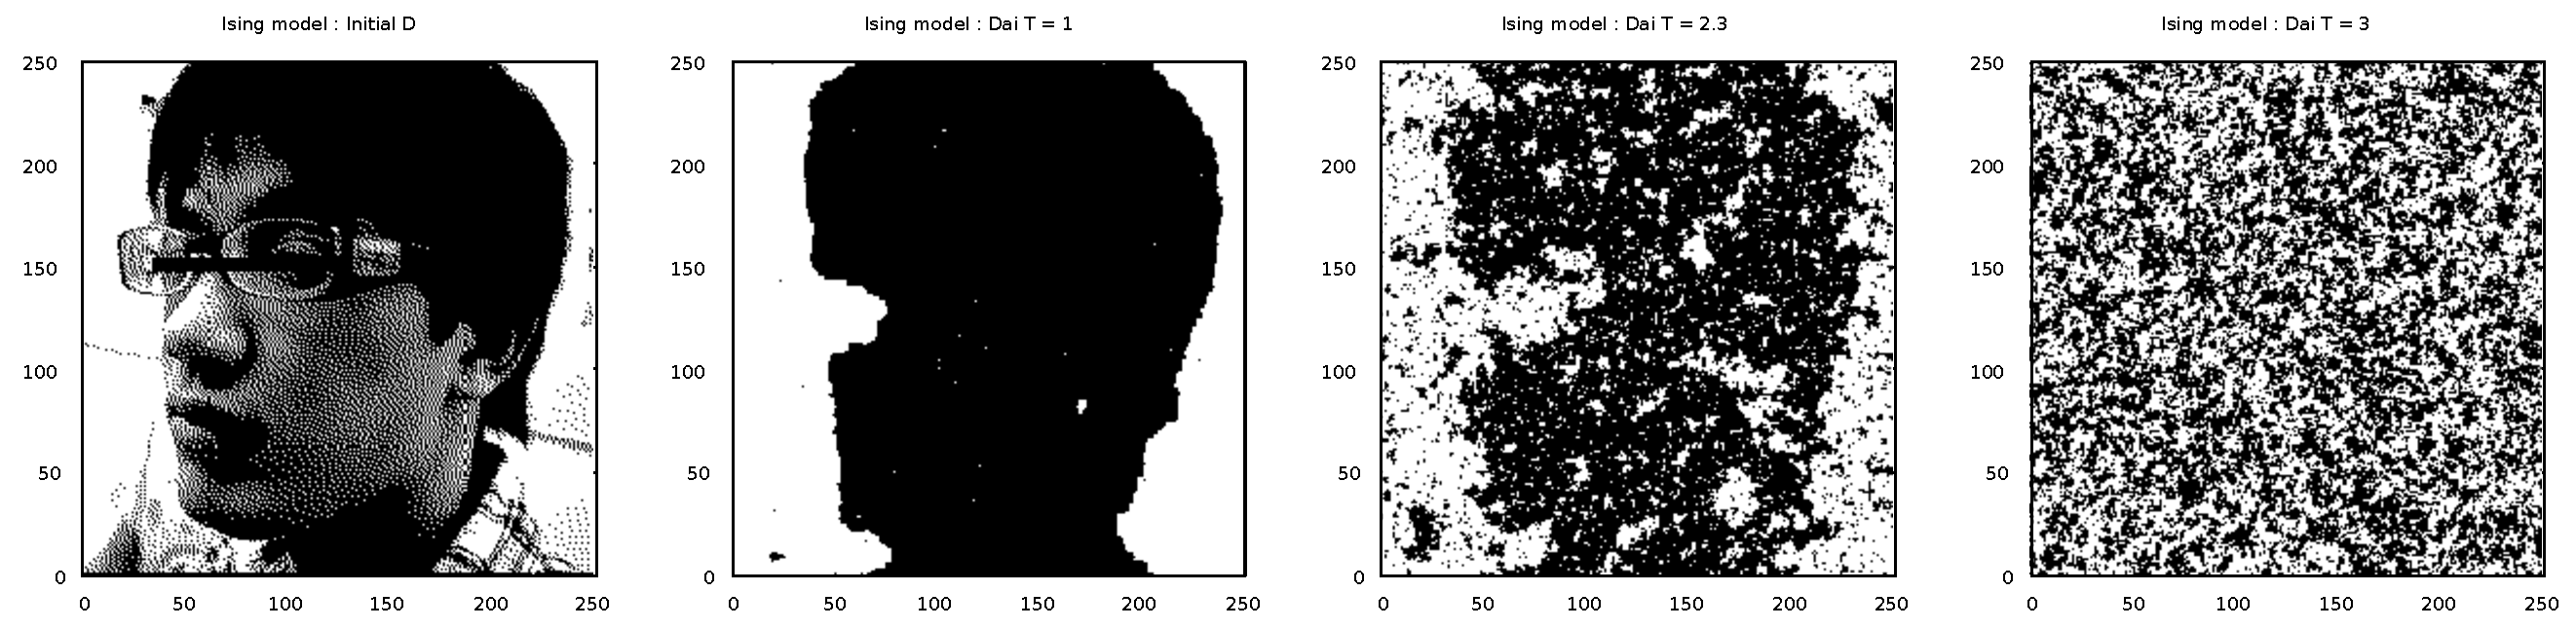
\includegraphics[width = 17cm]{./Dai.eps}
  \end{center}
  \label{Dai}
\end{figure}\\
ご覧の通り, Metropolis法だと磁化の形成は初期状態の選び方に強く依存します.

\newpage
\chapter{場の量子論}
\section{Wickの定理}
摂動計算において重要な役割を果たす. ただし, この定理が成立するのは\textbf{生成消滅演算子の代数を満たすものに限られる. }つまり, ゼロモード演算子はWickの定理を満たさない. 
\subsection{概要}
ざっくり言うと
\begin{screen}
  場の演算子の時間順序積(T積)はそれらの演算子から構成される全ての可能な正規積(N積)と伝搬関数の積の和で表される.
\end{screen}
伝搬関数(因果Green関数, Feynman propagator)は
\begin{eqnarray}
  \Delta_F(\bm{x}_1-\bm{x}_2, t_1-t_2) = -i\bra{0}{\rm T}\left[\phi(\bm{x}_1, t_1)\phi^\dagger(\bm{x}_2, t_2)\right]\ket{0}
\end{eqnarray}
で与えられるので, $\phi$の可能な組を全て足し上げればよい. 伝搬関数は$\phi^\dagger, \phi$の組で作られるので, $\phi\phi, \phi^\dagger\phi^\dagger$の組は考えなくても良い. 
N積は生成演算子を前に, 消滅演算子を後ろに持ってくる順序積:
\begin{eqnarray}
  :\phi_1\phi^\dagger_2\phi_3\phi^\dagger_4:\ = \phi^\dagger_2\phi^\dagger_4\phi_1\phi_3
\end{eqnarray}

大事なことは, \textbf{N積の真空期待値は必ずゼロになるということ}と, \textbf{演算子が時間に依存していないならば勝手にT積をつけてもよい}ということ. 期待値を計算するための面倒な交換関係計算があるとき, Wickが使えることがある. 基本的には伝搬関数が真空で作られているので有限温度では使えないが, 議論を有限温度期待値に拡張したBlock-de Dominicsの定理というのがある. 有限温度系におけるWickの定理とかも呼ばれる. 
\subsection{具体例}
\subsubsection{n=2の場合}
\begin{eqnarray}
  {\rm T}[\phi_1\phi_2] =\ :\phi_1\phi_2: + \bra{0}{\rm T}[\phi_1\phi_2]\ket{0}
\end{eqnarray}
\subsubsection{n=3の場合}
\begin{eqnarray}
  {\rm T}[\phi_1\phi_2\phi_3] =\ :\phi_1\phi_2\phi_3: + \bra{0}{\rm T}[\phi_1\phi_2]\ket{0}\phi_3 + \bra{0}{\rm T}[\phi_1\phi_3]\ket{0}\phi_2 + \bra{0}{\rm T}[\phi_2\phi_3]\ket{0}\phi_1 
\end{eqnarray}
\subsection{証明}
Fetterの章を参照のこと. 
\section{TFD形式による期待値計算}
$k$が連続自由度を持つ場合の期待値をTFDの力を借りて計算する.
\subsection{TFDのド基礎}
熱的真空は
\begin{eqnarray}
  \ket{0} &=& (1-f)\sum_mf^m\dket{m, m}\\
  \bra{0} &=& \sum_m\dbra{m, m}
\end{eqnarray}
で定義される. $f$はボルツマン因子. $f \neq e^{-\beta\omega}$のとき非平衡であるという. 熱的ブラ・ケットは双対ではない.
超演算子形式における$\dbra{I_R}\bullet\dket{\rho_R}$は熱的真空期待値$\ev{\bullet}{0}$に置き換えが可能\footnote{超演算子形式のチェック・チルダとTFDのノンチルダ・チルダは単射同型の関係にある. }. またBosonの熱的Bogoliubov変換の具体形は
\begin{eqnarray}
  b_{\bm{k}}^\dagger &=& \tilde{\xi_{\bm{k}}} + (1+n_{\bm{k}})\xi_{\bm{k}}^\dagger\\
  b_{\bm{k}} &=& \xi_{\bm{k}} + n_{\bm{k}}\tilde{\xi_{\bm{k}}}^\dagger
\end{eqnarray}
で与えられ, $\xi$演算子は熱的真空を消去する消滅演算子である:
\begin{eqnarray}
  \xi\ket{0} &=& \tilde{\xi}\ket{0} = 0\ ,\hspace{0.5cm} \bra{0}\xi^\dagger = \bra{0}\tilde{\xi}^\dagger = 0\\
  \comm{\xi}{\xi^\dagger} &=& \comm{\tilde{\xi_{\bm{k}}}}{\tilde{\xi_{\bm{k}'}}^\dagger} = \delta(\bm{k}-\bm{k}'), \hspace{0.5cm} \comm{\xi_{\bm{k}}}{\tilde{\xi_{\bm{k}'}}} = \comm{\xi_{\bm{k}}}{\tilde{\xi_{\bm{k}'}}^\dagger} = 0
\end{eqnarray}
この熱的真空, $\xi$演算子を用いて計算をする. 以下$x = (\bm{x}, t), y = (\bm{y}, s)$とする. 
\subsection{具体計算}
例として以下の計算をする:
\begin{eqnarray}
  \ev{R_3(x)R_3(y)} &\equiv& \bra{0}\frac{1}{(2\pi)^6}\int dk_1dk_2dk_3dk_4 b^\dagger_{k_1}b_{k_2}b^\dagger_{k_3}b_{k_4}e^{-i(k_1-k_2)x}e^{-i(k_3-k_4)y}e^{i(\omega_{k_1}-\omega_{k_2})t}e^{i(\omega_{k_3}-\omega_{k_4})s}\ket{0}\\
  \nonumber  &=& \frac{1}{(2\pi)^6}\int dk_1dk_2dk_3dk_4e^{-i(k_1-k_2)x}e^{-i(k_3-k_4)y}e^{i(\omega_{k_1}-\omega_{k_2})t}e^{i(\omega_{k_3}-\omega_{k_4})s}\\
  && \bra{0}\qty(\tilde{\xi_1} + (1+n_1)\xi_1^\dagger)\qty(\xi_2 + n_2\tilde{\xi_2}^\dagger)\qty(\tilde{\xi_3} + (1+n_3)\xi_3^\dagger)\qty(\xi_4 + n_4\tilde{\xi_4}^\dagger)\ket{0}
\end{eqnarray}
ここでは$\xi, n$の添字について$(k_1, k_2, k_3, k_4)\rightarrow(1, 2, 3, 4)$という置換をしている. 上式の熱的真空期待値を計算する:
\begin{eqnarray}
  &&\bra{0}\qty(\tilde{\xi_1} + (1+n_1)\xi_1^\dagger)\qty(\xi_2 + n_2\tilde{\xi_2}^\dagger)\qty(\tilde{\xi_3} + (1+n_3)\xi_3^\dagger)\qty(\xi_4 + n_4\tilde{\xi_4}^\dagger)\ket{0}\\
  =&&\bra{0}\tilde{\xi_1}\qty(\xi_2 + n_2\tilde{\xi_2}^\dagger)\qty(\tilde{\xi_3} + (1+n_3)\xi_3^\dagger)n_4\tilde{\xi_4}^\dagger\ket{0}\\
  =&&\bra{0}\qty(\tilde{\xi_1}\xi_2 + n_2\tilde{\xi_1}\tilde{\xi_2}^\dagger)\qty(n_4\tilde{\xi_3}\tilde{\xi_4}^\dagger + n_4(1+n_3)\xi_3^\dagger \tilde{\xi_4}^\dagger)\ket{0}\\
  =&&\bra{0}\qty(\tilde{\xi_1}\xi_2 + n_2\Bqty{\tilde{\xi_2}^\dagger\tilde{\xi_1} + \comm{\tilde{\xi_1}}{\tilde{\xi_2}^\dagger}})\qty(n_4\Bqty{\tilde{\xi_4}^\dagger\tilde{\xi_3} + \comm{\tilde{\xi_3}}{\tilde{\xi_4}^\dagger}} + n_4(1+n_3)\xi_3^\dagger \tilde{\xi_4}^\dagger)\ket{0}\\
  =&&\bra{0}\qty(\tilde{\xi_1}\xi_2 + n_2\delta(1-2))\qty(n_4\delta(3-4) + n_4(1+n_3)\xi_3^\dagger \tilde{\xi_4}^\dagger)\ket{0}\\
  \nonumber  = &&\bra{0}\qty(\tilde{\xi_1}\xi_2n_4\delta(3-4) + \tilde{\xi_1}\xi_2\xi_3^\dagger \tilde{\xi_4}^\dagger n_4(1+n_3) + n_2n_4\delta(1-2)\delta(3-4) + \xi_3^\dagger \tilde{\xi_4}^\dagger n_2n_4(1+n_3)\delta(1-2))\ket{0}\\
  \\
  = &&\bra{0}\qty(\tilde{\xi_1}\xi_2\xi_3^\dagger \tilde{\xi_4}^\dagger n_4(1+n_3) + n_2n_4\delta(1-2)\delta(3-4))\ket{0}\\
  = &&\bra{0}\Bqty{n_4(1+n_3)\delta(1-4)\delta(2-3) + n_2n_4\delta(1-2)\delta(3-4)}\ket{0}
\end{eqnarray}
よって
\begin{eqnarray}
  \nonumber  \ev{R_3(x)R_3(y)} &\equiv&\qty(\frac{1}{(2\pi)^3}\int dk n_k)^2 + \frac{1}{(2\pi)^6}\int dk_1dk_2 e^{-i(k_1-k_2)(x-y)}e^{i(\omega_{k_1}-\omega_{k_2})(t-s)}n_1(1+n_2)\label{expectation2}\\
\end{eqnarray}
\subsection{Block-de Dominicsの定理}
TFD形式だと計算が簡単になることがわかった\footnote{超演算子形式のままだとトレース演算になるのでなかなか面倒. }. ただ, 熱平均についてはBlock-de Dominicsの定理というWickの定理に対応するものがあるので, もっと簡単に計算できそうである. $b_1\sim b_6$まであるものを考えるが, $x, y$がcoupleするか否かは区別しないといけない\footnote{たとえば$1x-2x$がcoupleすると対応するデルタ関数$\delta(1-2)$が出てきて$e^{-i(k_1 - k_2)(x-y)}, e^{i(\omega_1 - \omega_2)(t-s)}$が消える.これは(\ref{expectation2})の右辺第一項にあたる項の起源. 一方で$x-y$のcross couplingがあるとexponentialの空間・時間成分が消えずに残る. これが(\ref{expectation2})の右辺第二項にあたる.}:
\begin{eqnarray}
  \ev{R_1(x)R_1^\dagger(y)} &\sim& \bra{0}b_{1x}^\dagger b^\dagger_{2x} b_{3x} b^\dagger_{4y} b_{5y} b_{6y} \ket{0} =\bra{0}{\rm T} \bqty{b_{1x}^\dagger b^\dagger_{2x} b_{3x} b^\dagger_{4y} b_{5y} b_{6y} }\ket{0}\\
  &=& 2\bra{0}{\rm T}\wick{321}{<1b_{1x}^\dagger <2b^\dagger_{2x} <3b_{3x} >3b^\dagger_{4y} >1b_{5y} >2b_{6y} }\ket{0} + 4\bra{0}{\rm T}\wick{321}{<1b_{1x}^\dagger <2b^\dagger_{2x} >1b_{3x} <3b^\dagger_{4y} >2b_{5y} >3b_{6y} }\ket{0}\\
  &=&2\ev{b^\dagger_{1x}b_{5y}}\ev{b^\dagger_{2x}b_{6y}}\ev{b_{3x}b^\dagger_{4y}} + 4\ev{b^\dagger_{1x}b_{3x}}\ev{b^\dagger_{2x}b_{5y}}\ev{b^\dagger_{4y}b_{6y}}\\
  \nonumber  &=& 2\delta(1-5)\delta(2-6)\delta(3-4)n_1n_2(1+n_3) + 4\delta(1-3)\delta(2-5)\delta(4-6)n_1n_2n_4\\
\end{eqnarray}
$\xi$演算子で真面目に計算しなくてもいける. 
\section{Gell-Mann-Lowの定理}
\subsection{断熱因子}
ハミルトニアンの摂動部が断熱因子を持っている場合を考える:
\begin{eqnarray}
  H = H_0 + e^{-\epsilon|t|}H_I
\end{eqnarray}
これは$t = 0$でfullの相互作用を取り入れた系になり, $t \rightarrow \pm\infty$で自由粒子になるようなハミルトニアンである. ここで, $t = t_0$かつ$t_0 \sim -\infty$で相互作用描像の状態が非摂動ハミルトニアンの固有状態になっている場合を考える\footnote{相互作用描像も自由粒子のハイゼンベルグ描像と一致するという近似できる. }:
\begin{eqnarray}
  H_0\ket{\Psi(t_0)}_I = E_0\ket{\Psi(t_0)}_I
\end{eqnarray}
さらに$t_0 \sim -\infty$であることから時間発展演算子を用いてハイゼンベルグ描像は
\begin{eqnarray}
  \ket{\Psi}_{\rm H} =  \ket{\Psi(0)}_I = U_\epsilon(0, t_0)\ket{\Psi(t_0)}_I= U_\epsilon(0, -\infty)\ket{\Psi(t_0)}_I\label{5eq1}
\end{eqnarray}
と書ける. これは, 相互作用系の状態が非摂動系の固有状態を用いて表現できたことを意味している.

あとは$\epsilon$について考える必要がある. そもそもこの系は2つの粒子の散乱実験をテーマにしたようなものである. 2つの粒子が$t = 0$で衝突することを考えるとき, 相互作用が効いてくるのは$t = 0$近傍のみであって, それ以外は自由粒子とほぼ同じ振る舞いをするだろうというアイデアから断熱因子は導入されている. 粒子を平面波的に記述するためにも$\epsilon\rightarrow 0$としたいが, この極限のもとで果たして(\ref{5eq1})は意味ある結果を与えるのだろうか?

これに答えるのがGell-Mann-Lowの定理である.\textbf{以降は基底状態に対する議論であることに注意.}
\subsection{概要}
Gell-Mann-Lowの定理が主張することは
\begin{eqnarray}
  \lim_{\epsilon\rightarrow0}\frac{U_\epsilon(0, -\infty)\ket{\phi_0(-\infty)}_I}{_I\bra{\phi_0(-\infty)}U_\epsilon(0, -\infty)\ket{\phi_0(-\infty)}_I} = \frac{\ket{\Psi_0}_H}{_I\expval{\phi_0(-\infty)|\Psi_0}_H}\label{gml}
\end{eqnarray}
が存在するなら固有状態$\ket{\Psi_0}_{\rm H}$はwell-definedであり, 固有値は
\begin{eqnarray}
  E-E_0 = \frac{_I\bra{\phi_0(-\infty)}H_I\ket{\Psi_0}_H}{_I\expval{\phi_0(-\infty)|\Psi_0}_H}
\end{eqnarray}
で与えられるということである. ここで添字の0は真空を意味している. また, $\ket{\phi_0(-\infty)}$は非摂動ハミルトニアンの固有状態になっているので解析的に求めることができる. あとは, (\ref{gml})が成立するかどうかが問題になる.

これが成立すればFree Hamiltonian $H_0$とFull Hamiltonian $H$をユニタリー演算子でつなぐことができる. つまり, Free Hamiltonianの固有状態$\ket{\Phi_0}$を求めたあとにユニタリー演算子$U(0, -\infty)$をAll orderで取り入れればFull Hamiltonianの固有状態が求まることになる. もちろんAll orderは無理なので摂動的に取り入れることになる. これが場の理論における摂動論である.

場の理論で物理量を摂動的に評価するときにはGreen関数を計算することが基本になるが, それを計算可能にするためのテクニックがWickの定理であり, そのWickの定理の証明にGell-Mann-Lowが用いられている. そういう意味でとっても重要. 
\subsection{証明}
Fetterの章を参照のこと. 
\section{Tips}
忘れやすいことをメモしておきます.
\subsection{Heisenberg描像}
Schr\"odinger描像は時間発展の情報が状態にある:
\begin{eqnarray}
  i\hbar\partial_t\ket{\psi(t)} &=& \hat{H}\ket{\psi(t)}\\
  \expval{\hat{A}} &=&\ _S\!\bra{\psi(t)}\hat{A}\ket{\psi(t)}_S
\end{eqnarray}
Schr\"odinger方程式の形式解
\begin{eqnarray}
  \ket{\psi(t)} = e^{-i\hat{H}t/\hbar}\ket{\psi(0)}
\end{eqnarray}
を用いると期待値は
\begin{eqnarray}
  \expval{\hat{A}} &=&\ _S\!\bra{\psi(0)}e^{i\hat{H}t/\hbar}\hat{A}e^{-i\hat{H}t/\hbar}\ket{\psi(0)}_S
\end{eqnarray}
と書くことができる. Heisenberg描像における演算子と状態は
\begin{eqnarray}
  \hat{A}_{\rm H}(t) &=& e^{i\hat{H}t/\hbar}\hat{A}e^{-i\hat{H}t/\hbar}\\
  \ket{\psi}_{\rm H} &=&  \ket{\psi(0)}_{\rm S}
\end{eqnarray}
\subsection{相互作用描像}
ハミルトニアンを
\begin{eqnarray}
  H = H_0 + H_I
\end{eqnarray}
のように非摂動部$H_0$と摂動部$H_I$に分割する. 分割の方法は任意だが, 非摂動部を解析的に解ける形にしておくのが普通\footnote{たとえば生成消滅演算子の2次で記述できればBogoliubov変換を通して対角化が可能. IZMFにおいては真空を$\ket{0}_{\rm ex}\ket{\Psi_0}$のように励起部とゼロモード部の直積にする. ゼロモードの真空は非摂動部にゼロモードの高次を取り込んで場の分割条件を守るようにカウンター項を決定する. ゼロモードは生成消滅演算子の代数を持っていないので取り扱いは励起部とは本質的に異なることに注意. }. Heisenberg描像の時と同じように形式解を代入する:
\begin{eqnarray}
  \ket{\psi(t)}_{\rm S} = e^{-i(\hat{H_0} + \hat{H_I})t/\hbar}\ket{\psi(0)}_{\rm S}
\end{eqnarray}
ここで, 相互作用描像の状態を
\begin{eqnarray}
  \ket{\psi(t)}_{\rm I} \equiv e^{i\hat{H_0}t/\hbar}\ket{\psi(t)}_{\rm S} &=& e^{-i\hat{H_I}t/\hbar}\ket{\psi(0)}_{\rm S}\\
  &=& e^{-i\hat{H_I}t/\hbar}\ket{\psi}_{\rm H}
\end{eqnarray}
と定義する. つまり, \textbf{相互作用描像の状態は摂動部$H_{\rm I}$(相互作用ハミルトニアン)による時間変化を担っている. }一方で相互作用描像の演算子は
\begin{eqnarray}
  A_{\rm I}(t) \equiv e^{i\hat{H_0}t/\hbar}\hat{A}_{\rm S}e^{-i\hat{H_0}t/\hbar}
\end{eqnarray}
で定義され, \textbf{非摂動部$H_0$による時間変化を担っている. }

この描像においては$t = 0$で真空はHeisenberg描像と一致し, 演算子の時間発展はHeisenberg方程式
\begin{eqnarray}
  i\hbar\partial_tA_{\rm I}(t) = [A_{\rm I}(t), H_0]
\end{eqnarray}
で記述される. ここで重要なのが, \textbf{演算子の時間発展は非摂動ハミルトニアンで記述されている}ということ. 演算子の時間発展を追うのは難しくなさそう\footnote{もちろん非摂動ハミルトニアンが解析的に解ける形である場合に限る}. 一方で状態の時間発展は
\begin{eqnarray}
  i\hbar\partial_t\ket{\psi(t)}_I = H_{\rm I}\ket{\psi(t)}_I
\end{eqnarray}
のように, 解析的に解けない相互作用ハミルトニアンで記述されているのでそんなに簡単ではない. よって, 状態は摂動展開によって評価することになる.
\subsection{各描像のハミルトニアン同士の関係}
\subsubsection{Full Hamiltonian}
Schr\"odinger描像とHeisenberg描像が一致:
\begin{eqnarray}
  H_H(t) = e^{iH_St}H_Se^{-iH_St} = H_S
\end{eqnarray}
これは任意の演算子については成立しないが, $t = 0$のときSchr\"odinger描像とHeisenberg描像は完全に一致する.
\subsubsection{Unperturbed Hamiltonian}
Schr\"odinger描像と相互作用描像が一致:
\begin{eqnarray}
  H_u(t) = e^{iH_{S, u}t}H_{S, u}e^{-iH_{S, u}t} = H_{S, u}
\end{eqnarray}
またHeisenberg描像とSchr\"odinger描像は
\begin{eqnarray}
  H_{H, u}(t) = e^{iH_St}H_{S, u}e^{-iH_St}
\end{eqnarray}
より, $t = 0$のときは非摂動部も一致する. $H_u(t)$は時間に依存しないことがわかっているので
\begin{eqnarray}
  H_u(t) &=& H_u(0) = H_{S, u}\\
  H_u(t) &=& H_u(0) = H_{S, u} = H_{H, u}(0)\hspace{0.7cm} where\ \ t = 0
\end{eqnarray}
である.
\subsection{デルタ関数のFourier変換表示}
1次元Fourier変換
\begin{eqnarray}
  f(x) &=& \frac{1}{\sqrt{2\pi}}\int dk \tilde{f}(k)e^{ikx}\\
  \tilde{f}(k) &=& \frac{1}{\sqrt{2\pi}}\int dx f(x)e^{-ikx}
\end{eqnarray}
を相互に代入する:
\begin{eqnarray}
  f(x) &=& \frac{1}{\sqrt{2\pi}}\int dk \left(\frac{1}{\sqrt{2\pi}}\int dx' f(x')e^{-ikx'}\right)e^{ikx}\\
  &=& \int dx' \left(\frac{1}{2\pi}\int dk e^{ik(x-x')}\right)f(x')
\end{eqnarray}
これより
\begin{eqnarray}
  \delta(x-x') &=& \frac{1}{2\pi}\int dk e^{ik(x-x')}\\
\end{eqnarray}
ひいては
\begin{eqnarray}
  \delta(x) &=& \frac{1}{2\pi}\int dk e^{ikx} = \frac{1}{2\pi}\int dk e^{-ikx}
\end{eqnarray}
であることがわかる. 「1のFourier変換は$2\pi\delta(x)$だ」という表現もできる. 
\subsection{$\bm{k}$が離散・連続の場合の$\expval{a_{\bm k}^\dagger a_{\bm{k}'}}$}
\subsubsection{有限体積の場合}
まずは$\left[\psi(x), \psi^\dagger(x')\right] = \delta(x - x')$を満たす一般的な演算子$\psi(x)$を離散変数$k_n$で展開した場合を考える. 体積$L$の一次元系について:
\begin{eqnarray}
  \psi(x) = \frac{1}{\sqrt{L}}\sum_{n=-\infty}^{n=\infty}e^{ik_nx}a_{k_n}
\end{eqnarray}
ただし$k_n = \frac{2\pi}{L}n$とする. すると,
\begin{eqnarray}
  \int dx\ \psi(x)e^{-ik_nx} &=& \frac{1}{\sqrt{L}}\sum_{n'}\int dx\ e^{-i(k_n-k_{n'})x}a_{k_{n'}}\\
  &=& \frac{1}{\sqrt{L}}\sum_{n'}L\delta_{nn'}a_{k_{n'}} = \sqrt{L}a_{k_n}\\
  \therefore a_{k_n} &=& \frac{1}{\sqrt{L}}\int dx\ \psi(x)e^{-ik_nx}  
\end{eqnarray}
このとき交換関係は
\begin{eqnarray}
  [a_{k_n}, a^\dagger_{k_{n'}}] = \frac{1}{L}\int dx dx'\ e^{-i(k_nx - k_{n'}x')}\left[\psi(x), \psi^\dagger(x')\right] = \frac{1}{L}\int dx \ e^{-i(k_n - k_{n'})x} = \delta_{nn'}
\end{eqnarray}
であり, 確かに本文の記述の通り,
\begin{eqnarray}
  \expval{a_{k_n}^\dagger a_{k_n}} = \frac{1}{e^{\beta\omega_{k_n}}-1} \equiv n_{k_n}
\end{eqnarray}
である.
\subsubsection{熱力学極限}
$L\rightarrow\infty$, つまり$k$の連続極限を取ることを考える. Fourier変換から
\begin{eqnarray}
  \psi(x) = \frac{1}{\sqrt{2\pi}}\int dk\ e^{ikx}a_k
\end{eqnarray}
となって欲しい. 交換関係が$[a_k, a_{k'}^\dagger] = \delta(k - k')$に変わる. これを守るために, $a_{k_n}\rightarrow ca_k$となる$c$を求める. $\sum_n\Delta ke^{ik_nx}\rightarrow\int dk e^{ikx}$かつ$\Delta k = \frac{2\pi}{L}$であることを用いて
\begin{eqnarray}
  \psi(x) = \frac{1}{\sqrt{L}}\sum_{n=-\infty}^{n=\infty}\frac{2\pi}{L}e^{ik_nx}a_{k_n}\frac{L}{2\pi}\rightarrow \frac{\sqrt{L}}{2\pi}\int dk e^{ikx} ca_n
\end{eqnarray}
となる. これより
\begin{eqnarray}
  c = \sqrt{\frac{2\pi}{L}}
\end{eqnarray}
以上より,
\begin{eqnarray}
  \expval{a_k^\dagger a_k} = \frac{L}{2\pi}n_k\label{particle}
\end{eqnarray}
であることがわかる. 今回は体積無限の系を考えているので,
\begin{eqnarray}
  \int_{-\infty}^\infty dx = L
\end{eqnarray}
であることから,
\begin{eqnarray}
  \delta(x) &=& \frac{1}{2\pi}\int dk\  e^{ikx}\\
  \Longrightarrow \delta(0) &=& \frac{1}{2\pi}\int dk = \frac{L}{2\pi}
\end{eqnarray}
つまり式(\ref{particle})はデルタ関数を用いて
\begin{eqnarray}
  \expval{a_k^\dagger a_k} = \delta(0)n_k\label{particle}
\end{eqnarray}
と表現できる.
\subsection{デルタ関数が体積になること}
\begin{eqnarray}
  \int^\infty_{-\infty} d\bm{x} = V
\end{eqnarray}
であり, デルタ関数のFourier変換表示
\begin{eqnarray}
  \delta(x) = \frac{1}{(2\pi)^3}\int dk e^{ikx}\hspace{0.5cm}\Longrightarrow \hspace{0.5cm}\delta(0) = \frac{1}{(2\pi)^3}\int dx = \frac{V}{(2\pi)^3}\label{delta-volume}
\end{eqnarray}
\subsection{ハミルトニアンの対角化とBogoliubov-de Gennes方程式}
\subsubsection{対角化とは}
ハミルトニアンの対角化とはハミルトニアンを生成消滅演算子を用いて
\begin{eqnarray}
  H = \sum_\ell \omega_{\ell} a_\ell a_\ell^\dagger\label{diagonal}
\end{eqnarray}
と表現することである. $\omega_\ell>0$であれば$a_\ell$が消去する$\ket{0}$が$H$の基底状態であることは量子力学における調和振動子の議論から明らか. $\omega_\ell < 0$である場合は$a_\ell$でいくらでもエネルギーを下げることができるので, $a_\ell$が張るFock空間には基底状態が存在しない\footnote{こういうのをLandau不安定性という. }.

正準交換関係を満たす場の演算子から生成消滅演算子を構成するのは簡単. 正規直交完全系$w_\ell$で場の演算子$\varphi$を展開する:
\begin{eqnarray}
  \varphi = \sum_\ell a_\ell(t)w_\ell(\bm{x}), \hspace{0.5cm} a_\ell = \int d\bm{x} \omega_\ell(\bm{x})\varphi(x)\label{expansion}
\end{eqnarray}
ただし
\begin{eqnarray}
  \sum_\ell w_\ell(\bm{x}) w^*_\ell(\bm{x}') = \delta(\bm{x}-\bm{x}'),\hspace{0.5cm}  \int d\bm{x} w_\ell(\bm{x}) w^*_{\ell'}(\bm{x}) = \delta_{\ell\ell'}
\end{eqnarray}
である. 
$\comm{\varphi(x)}{\varphi^\dagger(x')} = \delta(x - x')$から
\begin{eqnarray}
  \comm{a_\ell}{a^\dagger_{\ell'}} = \delta_{\ell\ell'}
\end{eqnarray}
であることがわかり, この$a, a^\dagger$は生成消滅演算子の代数を満たしている. つまり, 対角化のためには(\ref{diagonal})となるような適切な$w_\ell$を見つければ良い. $w_\ell$が変わると$a_\ell$の定義も変わるので, (\ref{expansion})で展開した時$a_\ell$が生成消滅演算子になるように構成しなければいけない. 

ここであるハミルトニアン
\begin{eqnarray}
  H_0 = \int d\bm{x} \varphi^\dagger(x)h_0(\bm{x})\varphi(x)\label{unperturb}
\end{eqnarray}
を対角化したい. $h_0$の固有値方程式
\begin{eqnarray}
  h_0(\bm{x})w_\ell(\bm{x}) = \omega_\ell w_\ell(\bm{x})
\end{eqnarray}
から正規直交完全系をつくり, それでもって$\varphi$を展開する:
\begin{eqnarray}
  H_0 &=& \int d\bm{x} \sum_{\ell\ell'}a^\dagger_\ell(t)w^*_\ell(\bm{x})h_0(\bm{x})w_{\ell'}(\bm{x})a_{\ell'}(t)\\
  &=& \int d\bm{x} \sum_{\ell\ell'}a^\dagger_\ell(t)w^*_\ell(\bm{x})\omega_{\ell'}w_{\ell'}(\bm{x})a_{\ell'}(t)\\
  &=& \sum_{\ell\ell'}\omega_{\ell'}a^\dagger_\ell(t)a_{\ell'}(t)\delta_{\ell\ell'}\\
  &=& \sum_{\ell}\omega_{\ell}a^\dagger_\ell(t)a_{\ell}(t)
\end{eqnarray}
対角化完了. つまり, (\ref{unperturb})のようなハミルトニアンは$h_0$の固有値問題を解き, その固有完全系でもって場の演算子を展開することで対角化ができる. これがほぼ唯一の対角化の方法である.
\subsubsection{Bogoliubov-de Gennes方程式}
冷却原子系のハミルトニアンの非摂動部をdoubletで書くと
\begin{eqnarray}
  H_u &=&  \int d\bm{x}
  \begin{pmatrix}
    \varphi^\dagger&-\varphi 
  \end{pmatrix}
  \begin{pmatrix}
    \calL &\calM\\
    -\calM^* &-\calL
  \end{pmatrix}
  \begin{pmatrix}
    \varphi\\
    \varphi^\dagger 
  \end{pmatrix}\\
  &=& \int d\bm{x} \overline{\Phi}T\Phi
\end{eqnarray}
となる\footnote{マイナスをつけたのはdoubletの$\Phi, \overline{\Phi}$が正準交換関係を満たすようにするため}. 先ほどのアナロジーから, $T$についての固有値方程式を解き, その固有関数系で$\Phi$を展開すれば非摂動部の対角化が可能である. この$T$についての固有値方程式がBogoliubov-de Gennes方程式である. $T$が一般にエルミートでないことに注意.
\subsection{一様系のBogoliubov-de Gennes方程式}
一様系ではBogoliubov変換とBogoliubov-de Gennes方程式による対角化は等価であり,解析的に計算が可能. 場の演算子をFourier変換:
\begin{eqnarray}
  \varphi = \frac{1}{\sqrt{(2\pi)^3}}\int d\bm{k} b_{\bm k}e^{i\bm{kx}}
\end{eqnarray}
ここで場を
\begin{eqnarray}
  \psi = \xi + \varphi
\end{eqnarray}
のように分割している. これを用いると冷却原子系の非摂動ハミルトニアンは
\begin{eqnarray}
  H_2 &=& \int d\bm{k}
  \begin{pmatrix}
    b_{\bm k}^\dagger &-b_{\bm -k} 
  \end{pmatrix}
  \begin{pmatrix}
    \calL_k &\calM\\
    -\calM^* &-\calL_k
  \end{pmatrix}
  \begin{pmatrix}
    b_{\bm k}\\
    b_{\bm -k}^\dagger 
  \end{pmatrix}
\end{eqnarray}
ただし
\begin{eqnarray}
  \calL_k &=& \varepsilon_k + gn_0,\ \calM = gn_0e^{2i\theta}\\
  \varepsilon_k &=& \frac{\hbar^2k^2}{2m},\ \xi(\bm{x}) = \sqrt{n_0}e^{i\theta},\ \mu = gn_0
\end{eqnarray}
つまり, k表示されたBdG行列の固有値問題を解けばよいことになり, さらに$\calL_k, \calM$は演算子を含まないので簡単である. これを解くと
\begin{eqnarray}
  \omega_k = \sqrt{\varepsilon_k(\varepsilon_k + 2gn_0)}
\end{eqnarray}
を得る.
\subsection{相互作用描像における時間発展演算子とT積}
相互作用描像の時間発展演算子が満たす方程式
\begin{eqnarray}
  i\hbar\partial_tU(t, 0)= H_I(t)U(t, 0)
\end{eqnarray}
について. 両辺を$t$で積分:
\begin{eqnarray}
  U(t, 0) = I + \qty(\frac{-i}{\hbar})\int_0^t dt_1 H_I(t_1)U(t_1, 0)
\end{eqnarray}
$U(0, 0) = I$としている. $U(t, 0)$を繰り返し代入する:
\begin{eqnarray}
  U(t, 0) &=& I + \qty(\frac{-i}{\hbar})\int_0^t dt_1 H_I(t_1)\qty(I + \qty(\frac{-i}{\hbar})\int_0^{t_1} dt_2 H_I(t_2)U(t_2, 0))\\
  &=& I + \qty(\frac{-i}{\hbar})\int_0^t dt_1 H_I(t_1) + \qty(\frac{-i}{\hbar})^2\int_0^t dt_1 \int_0^{t_1} dt_2 H_I(t_1)H_I(t_2)U(t_2, 0)\\
  \nonumber  &=& \cdots\\
  \nonumber&=& I + \qty(\frac{-i}{\hbar})\int_0^t dt_1 H_I(t_1) + \qty(\frac{-i}{\hbar})^2\int_0^t dt_1 \int_0^{t_1} dt_2 H_I(t_1)H_I(t_2)\\
  && \hspace{0.5cm}+ \cdots + \qty(\frac{-i}{\hbar})^n\int_0^t dt_1 \int_0^{t_1} dt_2\cdots\int_0^{t_{n-1}} dt_n H_I(t_1)H_I(t_2)\cdots H_I(t_n) + \cdots\label{T-product0}
\end{eqnarray}
このままだと積分の上端に変数が入っていて処理が難しいので変形する.

ある$H(t_1)H(t_2)$の二重積分について. ダミー変数$t_1\leftrightarrow t_2$の入れ替えでは値は変わらない:
\begin{eqnarray}
  && \int_0^t dt_1\int_0^{t_1}dt_2H(t_1)H(t_2) = \int_0^t dt_2\int_0^{t_2}dt_1H(t_2)H(t_1)\\
  &\therefore& \int_0^t dt_1\int_0^{t_1}dt_2H(t_1)H(t_2) + \int_0^t dt_2\int_0^{t_2}dt_1H(t_2)H(t_1) = 2\int_0^t dt_1\int_0^{t_1}dt_2H(t_1)H(t_2)\label{T-product1}
\end{eqnarray}
ここで唐突だが$H(t_1)H(t_2)$の時間順序積
\begin{eqnarray}
  T\qty[H(t_1)H(t_2)] = \theta(t_1 - t_2)H(t_1)H(t_2) + \theta(t_2 - t_1)H(t_2)H(t_1)
\end{eqnarray}
の積分を行う:
\begin{eqnarray}
\nonumber  \int_0^t dt_1\int_0^{t}dt_2 T\qty[H(t_1)H(t_2)] &=& \int_0^t dt_1\int_0^{t}dt_2\theta(t_1 - t_2)H(t_1)H(t_2) + \int_0^{t}dt_2\int_0^t dt_1\theta(t_2 - t_1)H(t_2)H(t_1)\\
  &=&\int_0^t dt_1\int_0^{t_1}dt_2H(t_1)H(t_2) + \int_0^{t}dt_2\int_0^{t_2} dt_1H(t_2)H(t_1)
\end{eqnarray}
(\ref{T-product1})の結果を用いると
\begin{eqnarray}
  \int_0^t dt_1\int_0^{t}dt_2 T\qty[H(t_1)H(t_2)] &=& 2\int_0^t dt_1\int_0^{t_1}dt_2H(t_1)H(t_2)
\end{eqnarray}
これを拡張すると
\begin{eqnarray}
  \int_0^t dt_1\int_0^{t}dt_2\int_0^{t}dt_3 T\qty[H(t_1)H(t_2)H(t_3)] &=& 3!\int_0^t dt_1\int_0^{t_1}dt_2\int_0^{t_2}dt_3H(t_1)H(t_2)H(t_3)\\
  \nonumber  \int_0^t dt_1\int_0^{t}dt_2\cdots\int_0^{t}dt_n T\qty[H(t_1)H(t_2)\cdots H(t_n)] &=& n!\int_0^t dt_1\int_0^{t_1}dt_2\cdots\int_0^{t_{n-1}}dt_nH(t_1)H(t_2)\cdots H(t_n)\\
\end{eqnarray}
となる. ここでは証明しないが帰納法でいけそう. これを用いて(\ref{T-product1})はT積を用いて
\begin{eqnarray}
\nonumber  U(t, 0) &=& I + \qty(\frac{-i}{\hbar})\int_0^t dt_1 H_I(t_1) + \frac{1}{2!}\qty(\frac{-i}{\hbar})^2\int_0^t dt_1 \int_0^{t} dt_2 T\qty[H_I(t_1)H_I(t_2)]\\
&& \hspace{0.5cm}+ \cdots + \frac{1}{n!}\qty(\frac{-i}{\hbar})^n\int_0^t dt_1 \int_0^{t} dt_2\cdots\int_0^{t} dt_n T\qty[H_I(t_1)H_I(t_2)\cdots H_I(t_n)] + \cdots\\
&=& \sum_{n}^\infty\frac{1}{n!}\qty(\frac{-i}{\hbar})^n\int_0^t dt_1 \int_0^{t} dt_2\cdots\int_0^{t} dt_n T\qty[H_I(t_1)H_I(t_2)\cdots H_I(t_n)]\label{T-product2}
\end{eqnarray}
のように書き換えられ, めでたく積分区間からダミー変数を除去できた. さらに, $dt_1, dt_2, \cdots dt_n$の積分順序は関係ないのでT積の中に入れ, かつ別々に積分を実行することができる:
\begin{eqnarray}
  U(t, 0) &=& \sum_{n}^\infty\frac{1}{n!}\qty(\frac{-i}{\hbar})^nT\qty[\int_0^t dt_1 \int_0^{t} dt_2\cdots\int_0^{t} dt_nH_I(t_1)H_I(t_2)\cdots H_I(t_n)]\\
  &=& \sum_{n}^\infty\frac{1}{n!}\qty(\frac{-i}{\hbar})^nT\qty[\int_0^t dt_1H_I(t_1) \int_0^{t} dt_2H_I(t_2)\cdots\int_0^{t} dt_nH_I(t_n)]\\
  &=& \sum_{n}^\infty\frac{1}{n!}\qty(\frac{-i}{\hbar})^nT\qty[\qty(\int_0^t ds H_I(s))^n]
\end{eqnarray}
それだけでなく, 時間が関係ない因子は全てT積に入れることができる:
\begin{eqnarray}
  U(t, 0) &=& T\qty[\sum_{n}^\infty\frac{1}{n!}\qty(\frac{-i}{\hbar})^n\qty(\int_0^t ds H_I(s))^n]\\
  &=& T\qty[\sum_{n}^\infty\frac{1}{n!}\qty(\frac{-i}{\hbar}\int_0^t ds H_I(s))^n]\\
  &=& T\exp(\frac{-i}{\hbar}\int_0^t ds H_I(s))
\end{eqnarray}
T積なんてこわくない!
\newpage
\chapter{研究 : 3次元一様有限温度系のゼロモード}
2015年度夏の学校. 有限温度ゼロモード系における自己無撞着計算がメイン. 有限温度系で重要な計算や考え方が頻出.

また, 夏の学校時点では凝縮粒子数の定義にゼロモード演算子の期待値を加えていなかったため, Depletionは相互作用定数$g$が小さいところで持ち上がる結果を得た. 凝縮粒子数の定義を変えたところ, Depletionは相互作用定数$g$に対してロバストになった. こっちのほうが自然だろうというのが今のところの結論. 
\section{問題設定}
粒子間の相互作用を考慮に入れてゼロモード演算子の期待値を計算をする.この効果のことを量子補正と呼ぶ.\\
相互作用がある場合はゼロ温度でも全ての粒子が凝縮するわけではないことから,今回は主に凝縮粒子数と非凝縮粒子数の割合(depletion)が相互作用によってどのように変わるか,またゼロモードの寄与がある場合とない場合で結果がどのように変わるかを見る.

まずは,量子補正を考慮した方程式の定式化から入る.
\subsection{冷却原子気体系のハミルトニアン}
冷却原子気体のハミルトニアンは以下のように与えられる.
\begin{eqnarray}
  H_{\rm H}=\int d\bm{x}\left[\psi_{\rm H}^\dagger(h_0-\mu)\psi_{\rm H} +\frac{g}{2}\psi_{\rm H}^\dagger\psi_{\rm H}^\dagger\psi_{\rm H}\psi_{\rm H}\right]
\end{eqnarray}
添字のHはHeisenberg描像であることを示している.$\mu$は化学ポテンシャル,$g$は相互作用定数,$h_0$は
\begin{eqnarray}
  h_0 = -\frac{\nabla^2}{2m}
\end{eqnarray}
であるような一様系を取り扱う.場の演算子$\psi_{\rm H}$は同時刻交換関係
\begin{eqnarray}
  &&\left[\psi_{\rm H}(\bm{x},t),\psi_{\rm H}^\dagger(\bm{x}',t) \right] = \delta(\bm{x} - \bm{x}')\\
  &&\left[\psi_{\rm H}(\bm{x},t),\psi_{\rm H}(\bm{x}',t) \right] = 0,\ \ \ \ \ \left[\psi_{\rm H}^\dagger(\bm{x},t),\psi_{\rm H}^\dagger(\bm{x}',t) \right] = 0
\end{eqnarray}
を満たす.このとき,$\psi_{\rm H}$は真空期待値を持つ:
\begin{eqnarray}
  \langle 0|\psi_{\rm H}(\bm{x})|0\rangle = \xi(\bm{x})\label{vaccum_ex1}
\end{eqnarray}
$\xi$は秩序変数と呼ばれ,$|\xi|^2$は凝縮体の密度と解釈できる.秩序変数は今回は時間に依存しないと仮定する.
場の演算子を以下のように分割する:
\begin{eqnarray}
  \psi_{\rm H} = \xi + \varphi_{\rm H}
\end{eqnarray}
$\xi$は凝縮体を記述する古典場,$\varphi_{\rm H}$は非凝縮体を記述する場の演算子と解釈できる.これは同時刻交換関係
\begin{eqnarray}
  \left[\varphi_{\rm H}(\bm{x},t),\varphi^\dagger_{\rm H}(\bm{x}',t)\right]  = \delta(\bm{x}-\bm{x}')\label{equal_time_commutation}
\end{eqnarray}
を満たしている.

ハミルトニアンを$\varphi_{\rm H}$の次数について整理すると
\begin{eqnarray}
  &&H_{{\rm H},1} = \int d\bm{x}\left[\varphi^\dagger_{\rm H}(h_0 - \mu + g|\xi|^2)\xi + \varphi_{\rm H}(h_0 - \mu + g|\xi|^2)\xi^*\right]\\
  &&H_{{\rm H},2} = \int d\bm{x}\left[\varphi^\dagger_{\rm H} {\cal L}\varphi_{\rm H} + \frac{1}{2}\varphi_{\rm H}{\cal M^*}\varphi_{\rm H}+\frac{1}{2}\varphi^\dagger_{\rm H}{\cal M}\varphi^\dagger_{\rm H}\right]\\
  &&H_{{\rm H},3} = g\int d\bm{x}\left[\xi^*\varphi^\dagger_{\rm H}\varphi_{\rm H}\varphi_{\rm H} + \xi\varphi^\dagger_{\rm H}\varphi^\dagger_{\rm H}\varphi_{\rm H} \right] \\
  &&H_{{\rm H},4} = \frac{g}{2}\int d\bm{x}\ \varphi^\dagger_{\rm H}\varphi^\dagger_{\rm H}\varphi_{\rm H}\varphi_{\rm H}
\end{eqnarray}
であり
\begin{eqnarray}
  {\cal L} = h_0 - \mu +2g|\xi|^2,\ \ \ \ \ {\cal M}=g\xi^2
\end{eqnarray}
である.

\subsection{相互作用描像}
系が十分低温であり相互作用$g$が小さいとする.この場合$H_{{\rm H},3},H_{{\rm H},4}$の効果は小さいとして,非摂動ハミルトニアンを$H_{{\rm H},u}=H_{{\rm H},1}+H_{{\rm H},2}$のように選び,Heisenberg描像から相互作用描像に移行する.まず
\begin{eqnarray}
  i\frac{d}{dt}U(t,t_0)=U(t,t_0)H_{{\rm H},p},\ \ \ \ \ U(t_0,t_0)=1,\ \ \ \ \ H_{{\rm H},p} = H_{\rm H} - H_{{\rm H},u}
\end{eqnarray}
を満たすようなユニタリー演算子$U(t,t_0)$を考え,Heisenberg描像の任意の演算子$A_{\rm H}(t)$を用いて相互作用描像の演算子を
\begin{eqnarray}
  A(t) = U(t,t_0)A_{\rm H}(t)U^{-1}(t,t_0)
\end{eqnarray}
と定義する.$t_0$はHeisenberg描像と相互作用描像が一致する時間である.Heisenberg方程式は
\begin{eqnarray}
  i\frac{d}{dt}A(t) = \left[A(t),H_u(t)\right]
\end{eqnarray}
である.ここで$A=H_u$と代入すると時間に依存しないことがわかるので,$H_u = H_{{\rm H},u}$である.

$U(t,t_0)$の時間発展は$H_{{\rm H},p}=H_{{\rm H},3}+H_{{\rm H},4}$に依存し,かつその効果が小さいことから場の演算子の摂動ゼロ次は
\begin{eqnarray}
  \langle0|\varphi_{\rm H}(x)|0\rangle = \langle0| U^{-1}(t,t_0)\varphi(x)U(t,t_0)|0\rangle \simeq \langle0|\varphi(x)|0\rangle
\end{eqnarray}
となっている.また相互作用描像のHeisenberg方程式より
\begin{eqnarray}
  i\frac{\partial}{\partial t}\varphi(x) = \left[\varphi(x),H_u\right]\label{Heisenberg}
\end{eqnarray}
であることがわかる.これ以降$x=(\bm{x},t)$とする.つまり,場の分割条件を
\begin{eqnarray}
  \langle0|\varphi_{\rm H}(x)|0\rangle \simeq \langle0|\varphi(x)|0\rangle = 0
\end{eqnarray}
とした場合,この性質が保存するためには式(\ref{Heisenberg})より
\begin{eqnarray}
  \bra{0}\left[\varphi(x),H_u\right]\ket{0} = 0
\end{eqnarray}
が必要となる.ここから定常Gross-Pitaevskii方程式(GP方程式)
\begin{eqnarray}
  \left[h_0 - \mu +g|\xi|^2\right]\xi = 0\label{GP}
\end{eqnarray}
が導かれる.
\subsection{量子補正}
量子補正を取り入れる場合は場の分割条件を$\bra{0}[\varphi,H_u]\ket{0}=0$ではなく
\begin{eqnarray}
  \bra{0}[\varphi,H]\ket{0} = 0 \label{split}
\end{eqnarray}
とする.これはもともとの場の分割条件$\bra{0}\varphi_H\ket{0} = 0$の摂動1次までを取り入れたことになっている\footnote{実は正確な表現ではない. }.これを具体的に計算する:
\begin{eqnarray}
  \nonumber  \bra{0}[\varphi,H_1]\ket{0} &=& \bra{0}\int d\bm{x}\left[\varphi,\left\{\varphi^\dagger{\cal L}\xi+\varphi{\cal L}\xi^*\right\}\right]\ket{0}\\
  &=& (h_0 - \mu + g|\xi|^2)\xi\\
  \nonumber  \bra{0}[\varphi,H_2]\ket{0} &=& \bra{0}\int d\bm{x}\left[\varphi,\left\{\varphi^\dagger{\cal L}\varphi+\frac{1}{2}\varphi{\cal M}^*\varphi + \frac{1}{2}\varphi^\dagger{\cal M}\varphi^\dagger\right\}\right]\ket{0}\\
  &=& \bra{0}{\cal L}\varphi + {\cal M}\varphi^\dagger \ket{0} = 0\\
  \nonumber  \bra{0}[\varphi,H_3]\ket{0} &=& \bra{0}g\int d\bm{x}\left[\varphi,\left\{\xi^*\varphi^\dagger\varphi\varphi + \xi\varphi^\dagger\varphi^\dagger\varphi \right\}\right]\ket{0}\\
  &=& g\bra{0}\varphi\varphi\ket{0}\xi^* + 2g\bra{0}\varphi^\dagger\varphi\ket{0}\xi\\
  \nonumber  \bra{0}[\varphi,H_4]\ket{0} &=& \bra{0}\frac{g}{2}\int d\bm{x}\left[\varphi,\varphi^\dagger\varphi^\dagger\varphi\varphi\right]\ket{0}\\
  &=& g\bra{0}\varphi^\dagger\varphi\varphi\ket{0}
\end{eqnarray}
ここで$\varphi$の3次の期待値の寄与は小さいものとすると,式(\ref{split})より
\begin{eqnarray}
  \left[h_0 - \mu + g|\xi|^2 + 2g\bra{0}\varphi^\dagger\varphi\ket{0}\right]\xi + g\bra{0}\varphi\varphi\ket{0}\xi^* = 0
\end{eqnarray}
これが量子補正を考慮したGP方程式である.ここでゼロモード部と励起部に分けて記述すると
\begin{eqnarray}
 \nonumber \bra{0}\varphi^\dagger\varphi\ket{0} &=& _{\rm ex}\bra{0}\varphi^\dagger_{\rm ex}\varphi_{\rm ex}\ket{0}_{\rm ex} + |\xi|^2\bra{\Psi}Q^2\ket{\Psi} + |\eta|^2\bra{\Psi}P^2\ket{\Psi} \\
  &&\ \ \ \ \ \ \ \ -{\rm Re}\xi^*\eta -{\rm Im}\xi^*\eta(QP + PQ)\\
\nonumber  \bra{0}\varphi\varphi\ket{0} &=& _{\rm ex}\bra{0}\varphi_{\rm ex}\varphi_{\rm ex}\ket{0}_{\rm ex} - \xi^2\bra{\Psi}Q^2\ket{\Psi} + \eta^2\bra{\Psi}P^2\ket{\Psi} \\
  &&\ \ \ \ \ \ \ \ -i\xi\eta\bra{\Psi}QP + PQ\ket{\Psi}
\end{eqnarray}
となる.ここで$\varphi = -iQ\xi + P\eta + \varphi_{\rm ex}$とし,かつ$\ket{0} = \ket{0}_{\rm ex}\otimes\ket{\Psi}$としている.$Q,P$は正準交換関係$[Q,P] = i$を満たすゼロモード演算子,非摂動ハミルトニアン$H_u$の励起部$H_u^{\rm ex}$,ゼロモード部$H_u^{QP}$の固有状態をそれぞれ$\ket{0}_{\rm ex},\ket{\Psi}$である.

GP方程式が補正を受けたので,Bogoliubov-de Gennes方程式(BdG方程式)にも補正を加える.具体的には
\begin{eqnarray}
  {\cal L} &=&  h_0 - \mu + 2g(|\xi|^2 + \bra{0}\varphi^\dagger\varphi\ket{0})\label{L}\\
  {\cal M} &=& g(\xi^2 - \bra{0}\varphi\varphi\ket{0})\label{M}
\end{eqnarray}
となっていれば$\bm{y}_0 = \begin{pmatrix}\xi & -\xi^*  \end{pmatrix}$がゼロモードであることを守れる.ここで非摂動ハミルトニアンを
\begin{eqnarray}
  H_u = H_1 + H_2 + [H_3 + H_4]_{QP} -\delta\mu P -\delta\nu Q + \delta H
\end{eqnarray}
と取り,カウンター項$\delta H$を
\begin{eqnarray}
  \delta H = g\int d\bm{x}\left[2\varphi^\dagger\varphi\bra{0}\varphi^\dagger\varphi\ket{0}-\frac{1}{2}\varphi\varphi\bra{0}\varphi^\dagger\varphi^\dagger\ket{0}-\frac{1}{2}\varphi^\dagger\varphi^\dagger\bra{0}\varphi\varphi\ket{0}\right]
\end{eqnarray}
と選ぶことで,$H_u^{QP}$は量子補正を考慮しない場合と同じ形を取ることができる.式(\ref{L})(\ref{M})より共役モード方程式$
\begin{pmatrix}
  {\cal L} & {\cal M}\\
  -{\cal M}&-{\cal L}
\end{pmatrix}
\bm{y}_{-1}=I\bm{y}_0
$は
\begin{eqnarray}
  \left[h_0 - \mu + 2g(|\xi|^2 + \bra{0}\varphi^\dagger\varphi\ket{0})\right]\eta + g(\xi^2 - \bra{0}\varphi\varphi\ket{0})\eta^*=I\xi
\end{eqnarray}
となる.以上の定式化を用いて各物理量の計算を行っていく.
\section{自己無撞着ループ}
前節で導いた関係式に現れる物理量は自己無撞着に決定されるが,その関係式同士のつながりは複雑である.
以下では3次元一様有限温度系に現れる自己無撞着ループについてまとめる.2章のはなしを有限温度に拡張するために期待値のとり方を変えていることに注意.
\\

\begin{itembox}[c]{0. 初期設定}
  \begin{center}
    $V_t = \ev{\varphi^{\dagger}\varphi} = 0$, $V_a = \ev{\varphi\varphi} = 0$からスタート
  \end{center}
\end{itembox}

\begin{center}
  $\Downarrow$
\end{center}

\begin{itembox}[c]{1. GP方程式}
  \begin{center}
    GP方程式より$\xi, \mu $を求める
  \end{center}
\end{itembox}

\begin{center}
  $\Downarrow$
\end{center}

\begin{itembox}[c]{2. 共役モード方程式}
  \begin{center}
    共役モード方程式より$\eta, I$を求める
  \end{center}
\end{itembox}

\begin{center}
  $\Downarrow$
\end{center}

\begin{itembox}[c]{3. BdG方程式}
  \begin{center}
    BdG方程式(Bogoliubov変換)より$u_l, v_l$を求める
  \end{center}
\end{itembox}

\begin{center}
  $\Downarrow$
\end{center}

\begin{itembox}[c]{4. ゼロモード方程式}
  \begin{center}
    ゼロモード方程式より固有関数$\ev{q|\Psi}$を求め,$\ev{P}$を求める\\
    $\Updownarrow$\\
    $\ev{P} = 0$となるように自己無撞着に$\delta\mu$を決定
  \end{center}
\end{itembox}

\begin{center}
  $\Downarrow$
\end{center}

\begin{itembox}[c]{5. ゼロモード演算子}
  \begin{center}
    $\ev{Q^2}, \ev{P^2}$を求める
  \end{center}
\end{itembox}

\begin{center}
  $\Downarrow$
\end{center}

\begin{itembox}[c]{6. 熱平均・異常平均}
  \begin{center}
    $V_t, V_a$を求める.
  \end{center}
\end{itembox}

\begin{center}
  $\Downarrow$
\end{center}

\begin{itembox}[c]{ループ/終了条件}
  \begin{center}
    「1. GP方程式」 に戻って計算を繰り返す.$V_t, V_a$の値が変化しなくなったら終了.
  \end{center}
\end{itembox}

\subsection{GP方程式}
入力:$V_t,V_a$

$\xi,\eta$は実数とする.量子補正を含むGP方程式は
\begin{eqnarray}
  [-\mu + g\xi^2 + g(2V_t + V_a)]\xi = 0
\end{eqnarray}  
である.今回は一様系を扱うため微分項$h_0$がなくなり,簡単な代数方程式になる.これを$\mu$について解く:
\begin{eqnarray}
  \mu = g(\xi^2 + 2V_t + V_a)
\end{eqnarray}
ここで粒子数$N$が保存するためには
\begin{eqnarray}
  \nonumber  N &=& \int d\bm{x}\ev{\psi^\dagger\psi}\\
  \nonumber  &=& \int d\bm{x}\ev{(\xi + \varphi^\dagger)(\xi + \varphi)}\\
  &=& V(\xi^2 + V_t)
\end{eqnarray}
を満たさなければならない.ここでは分割条件から$\ev{\varphi},\ev{\varphi^\dagger}$はゼロになっている.したがって,
\begin{itembox}[c]{GP方程式}
\begin{eqnarray}
  \xi &=& \sqrt{\frac{N}{V} - V_t}\\
  \mu &=& g(\frac{N}{V} + V_t + V_a)
\end{eqnarray}
\end{itembox}
となることがわかる.

\subsection{共役モード方程式}
入力:$V_a, V_t, \xi, \mu$

量子補正を含む共役モード方程式は
\begin{eqnarray}
  [-\mu + g(3\xi^2 + 2V_t - V_a)]\eta = I\xi 
\end{eqnarray}
である.GP方程式と同様の理由で代数方程式となっている.これを$I$について解く:
\begin{eqnarray}
  I = \frac{\eta}{\xi}[-\mu + g(3\xi^2 + 2V_t - V_a)]
\end{eqnarray}
ここでゼロモードと共役モードの規格化条件から
\begin{eqnarray}
  \nonumber  (\bm{y}_0, \bm{y}_{-1}) &=& \int d\bm{x}
  \begin{pmatrix}
    \xi & -\xi
  \end{pmatrix}
  \begin{pmatrix}
    1 & 0\\
    0 & -1
  \end{pmatrix}
  \begin{pmatrix}
    \eta\\
    \eta
  \end{pmatrix}\\
  &=& 2V\xi\eta = 1
\end{eqnarray}
を満たさなければならない.したがって
\begin{itembox}[c]{共役モード方程式}
\begin{eqnarray}
  \eta &=& \frac{1}{2V\xi}\\
  I &=& \frac{-\mu + g(3\xi + 2V_t - V_a)}{2V\xi^2}
\end{eqnarray}
\end{itembox}
となることがわかる.

\subsection{BdG方程式}
入力:$V_a, V_t, \xi, \mu$

一様系ではBogoliubov変換から$u_l,v_l$を求めることができる.

\begin{eqnarray}
  \varphi = \frac{1}{(2\pi)^{3/2}}\int d\bm{k}\ b_{\bm{k}}e^{i\bm{k}\bm{x}}
\end{eqnarray}
と展開すると,ハミルトニアンの2次$H_2$は
\begin{eqnarray}
  H_2 = \frac{1}{2}\int d\bm{k}\ [2{\cal L}_kb^\dagger_{\bm{k}}b_{\bm{k}} + {\cal M}(b^\dagger_{\bm{k}}b^\dagger_{-\bm{k}} + b_{\bm{k}}b_{-\bm{k}})]
\end{eqnarray}
とかける.ただし
\begin{eqnarray}
  {\cal M} &=& g(\xi^2 - V_a)\\
  \nonumber  {\cal L}_k &=& \frac{\hbar^2}{2m}k^2 - \mu + 2g(\xi^2 + V_t)\\
  &=& \frac{\hbar^2}{2m}k^2 + {\cal M}
\end{eqnarray}
である.ここで
\begin{eqnarray}
  H_2 = \int d\bm{k}\ \omega_ka^\dagger_{\bm k}a_{\bm k}
\end{eqnarray}
となるような
\begin{eqnarray}
  a_{\bm k} = u_kb_{\bm k} - v_kb_{-\bm{k}}\label{operator}
\end{eqnarray}
を満たす$u_k$, $v_k$を探す.$a_k$は生成消滅演算子の代数を満たさなければならないので
\begin{eqnarray}
  |u_k|^2-|v_k|^2=1
\end{eqnarray}
が必要であり,式(\ref{operator})を$b$について解いて$H_2$に代入することにより,対角化の条件は
\begin{eqnarray}
  2{\cal L}_ku_kv_k -{\cal M}(u^2_k + v^2_k) = 0
\end{eqnarray}
であることがわかる.これらを連立させることにより
\begin{itembox}[c]{Bogoliubov変換}
\begin{eqnarray}
  \begin{pmatrix}
      u_k\\
      v_k
    \end{pmatrix}
  &=& \frac{1}{\sqrt{2\omega_k}}
  \begin{pmatrix}
    \sqrt{{\cal L}_k + \omega_k}\\
    -\sqrt{{\cal L}_k - \omega_k}
  \end{pmatrix}\\
  \omega_k &=& \sqrt{{\cal L}^2_k - {\cal M}^2}
\end{eqnarray}
\end{itembox}
を得る.
\subsection{ゼロモード方程式}
入力:\ $\xi, \eta, I$

今回考えるゼロモード方程式は以下:
\begin{eqnarray}
  H_u^{QP}\ket{\Psi_m} = E_m\ket{\Psi_m}
\end{eqnarray}
ただし
\begin{eqnarray}
  \nonumber  H_u^{QP} = -(\delta\mu + 4C)P &+& \frac{I-4D}{2}P^2 + 2BQPQ + 2DP^3\\
  &+& \frac{1}{2}AQ^4 -2BQ^2 + CQP^2Q + \frac{1}{2}EP^4
\end{eqnarray}
である.これを$q$空間で差分化して数値的に解く.$q$空間での波束の幅はおよそ$N_0^{-1/3}$のオーダーであることを基に系のサイズを決める.
\\
\begin{eqnarray}
  \Psi_q = \sqrt{\Delta q}\ev{q|\Psi}
\end{eqnarray}
として差分化すると,ハミルトニアン$H_u^{QP}$は以下のようになる
\begin{eqnarray}
  H_u^{QP} =
  \begin{pmatrix}
    \alpha_0 & \beta_0& \gamma_0& & & \\
    \beta_0^* & \alpha_1 & \beta_1 & \gamma_1 & & \\
    \gamma_0^* &\beta_1^* &\alpha_2 &\beta_2 &\gamma_2 &\\
    &\gamma_1^* & \beta_2^* & \alpha_3 & \ddots & \ddots\\
    & & \gamma_2^* & \ddots &\ddots &\ddots \\
    &&&\ddots &\ddots &\ddots 
  \end{pmatrix}
\end{eqnarray}
\begin{eqnarray}
  \alpha_q &=& \frac{3E}{\Delta q^4} + \frac{I-4D}{\Delta q^2} + (2C -2\Delta q^2B)(q-\frac{N_q}{2})^2 + \frac{\Delta q^4}{2}Aq^4 \\
  \beta_q &=& -\frac{2E}{\Delta q^4} - \frac{2iD}{\Delta q^3} - \frac{I-4D}{2\Delta q^2} + \frac{i(\delta\mu + 4C)}{2\Delta q} - (C + i\Delta qB)(q - \frac{N_q}{2})(q - \frac{N_q}{2}+1)\\
  \gamma_q &=& \frac{E}{2\Delta q^4} + \frac{iD}{\Delta q^3}
\end{eqnarray}
有限温度系での期待値の取り方に注意すると
\begin{eqnarray}
  \nonumber  \ev{P} &=& \frac{{\rm Tr}\rho P}{{\rm Tr}\rho}\\
  \nonumber &=& \frac{\sum_m\bra{\Psi_m} P \ket{\Psi_m}e^{-\beta E_m}}{\sum_me^{-\beta E_m}}\\
  &=& \frac{\sum_m\sum_q{\rm Im} \Psi_q^{*,m}\Psi_{q+1}^me^{-\beta E_m}}{\Delta q\sum_me^{-\beta E_m}}
\end{eqnarray}
ただし密度演算子$\rho$は
\begin{eqnarray}
  \rho = e^{-\beta H_u^{QP}}
\end{eqnarray}
である.場の分割条件から$\ev{P} = 0$を満たさなければならないので,それに合わせて自己無撞着的に$\delta\mu$を決定することになる.数値計算上では二分法を用いる.

\subsection{$\ev{Q^2},\ev{P^2}$の計算}

前節で決定された$\delta \mu$を基に求めたゼロモード固有関数$\Psi^m_q$を用いて$\ev{P}$と同様の計算で$\ev{Q^2},\ev{P^2}$を求める.
\begin{itembox}[c]{ゼロモード演算子の有限温度期待値}
\begin{eqnarray}
  \ev{Q^2}&=& \frac{\Delta q^2\sum_m\sum_q(q - \frac{N_q}{2})|\Psi_q^m|^2e^{-\beta E_m}}{\sum_me^{-\beta E_m}}\\
  \ev{P^2}&=& \frac{2\sum_m\sum_q(|\Psi_q^m|^2-{\rm Re}\Psi_q^{*,m}\Psi_{q+1}^m)e^{-\beta E_m}}{\Delta q^2\sum_me^{-\beta E_m}}
\end{eqnarray}
\end{itembox}

\subsection{熱平均$V_t$・異常平均$V_a$}
入力:$\xi, \eta, u_l, v_l, \ev{Q^2}, \ev{P^2}$

熱平均・異常平均は以下の通り:
\begin{eqnarray}
  V_t = \ev{\varphi^\dagger\varphi} &=& _{{\rm ex}}\ev{\varphi^\dagger_{{\rm ex}}\varphi_{{\rm ex}}}_{{\rm ex}} + \xi^2\ev{Q^2} + \eta^2\ev{P^2} -\xi\eta \\
  %  &=& \sum_l\left[\frac{1}{e^{\beta\omega_l}-1}(|u_l|^2 + |v_l|^2)\right] + \xi^2\ev{Q^2} + \eta^2\ev{P^2} -\xi\eta 
  V_a = \ev{\varphi\varphi} &=& _{{\rm ex}}\ev{\varphi_{{\rm ex}}\varphi_{{\rm ex}}}_{{\rm ex}} - \xi^2\ev{Q^2} + \eta^2\ev{P^2} + i\xi\eta\ev{QP+PQ} 
  %  &=& \sum_l\left[\left(\frac{2}{e^{\beta\omega_l}-1}+1\right)u_lv^*_l\right] - \xi^2\ev{Q^2} + \eta^2\ev{P^2} + i\xi\eta\ev{QP+PQ} 
\end{eqnarray}
$\varphi_{\rm ex}$を以下のように展開する:
\begin{eqnarray}
  \varphi_{\rm ex} = \frac{1}{\sqrt{(2\pi)^3}}\int^{\infty}_{-\infty} d\bm{k}[a_{\bm{k}}u_k + a^\dagger_{-\bm{k}} v_k^*]e^{i\bm{k}\bm{x}}
\end{eqnarray}
ここで$a_{\bm{k}}$が消去する真空を$\ket{0}_k$,粒子数状態を
\begin{eqnarray}
  \ket{n} = \ket{n_1}_1\otimes\ket{n_2}_2\otimes\ket{n_3}_3\otimes... = \underset{k}{\otimes}\ket{n_k}_k
\end{eqnarray}
とする.

以上から$_{\rm ex}\ev{\varphi^\dagger_{{\rm ex}}\varphi_{{\rm ex}}}_{\rm ex},\  _{\rm ex}\ev{\varphi_{{\rm ex}}\varphi_{{\rm ex}}}_{\rm ex}$の計算をしていくために励起モードの期待値計算についてまとめる.
\begin{eqnarray}
  _{\rm ex}\ev{A}_{\rm ex} = \frac{{\rm Tr}\rho A}{{\rm Tr}\rho},\ \ \ \ \ \rho = e^{-\beta H^{\rm ex}_u}
\end{eqnarray}
であり
\begin{eqnarray}
  \nonumber  {\rm Tr}\rho &=& \sum_{n_1}\sum_{n_2}...\bra{n}e^{-\beta\sum_k\omega_{\bm{k}}a^\dagger_{\bm{k}}a_{\bm{k}}}\ket{n} = \sum_{n_1}\sum_{n_2}...\bra{n}e^{-\beta\sum_k\omega_{\bm{k}}n_{\bm{k}}}\ket{n} = \sum_{n_1}\sum_{n_2}...\prod_ke^{-\beta\omega_{\bm{k}}n_{\bm{k}}}\\
  &=& \prod_k\sum_{n_1}\sum_{n_2}...e^{-\beta\omega_{\bm{k}}n_{\bm{k}}} = \prod_k\sum_{n_{\bm{k}}}e^{-\beta\omega_{\bm{k}}n_{\bm{k}}} = \prod_k\frac{1}{1-e^{-\beta\omega_{\bm{k}}}}
\end{eqnarray}
\begin{eqnarray}
  \nonumber  {\rm Tr}\rho a^\dagger_{\bm k}a_{\bm{k}} &=& \sum_{n_1}\sum_{n_2}...\bra{n}e^{-\beta\sum_k\omega_{\bm{k}}a^\dagger_{\bm k}a_{\bm{k}}}a^\dagger_{\bm k}a_{\bm{k}}\ket{n} = \sum_{n_1}\sum_{n_2}...\left(\prod_{l\neq k}e^{-\beta\omega_ln_l}\right)n_le^{-\beta\omega_ln_l}\\
  \nonumber  &=& \prod_{l\neq k}\left(\sum_{n_1}\sum_{n_2}...\sum_{n_{l-1}}\sum_{n_{l+1}}...e^{-\beta\omega_ln_l}\right)\sum_kn_{\bm{k}}e^{-\beta\omega_{\bm{k}}n_{\bm{k}}} = \left(\prod_{k\neq l}\sum_{n_{\bm{k}}}e^{-\beta\omega_ln_l}\right)\sum_kn_{\bm{k}}e^{-\beta\omega_{\bm{k}}n_{\bm{k}}}\\
  &=&\left(\prod_{l\neq k}\frac{1}{1-e^{-\beta\omega_l}}\right)\frac{e^{-\beta\omega_{\bm{k}}}}{(1-e^{-\beta\omega_{\bm{k}}})^2}
\end{eqnarray}
から,
\begin{eqnarray}
  \nonumber  _{\rm ex}\ev{a^\dagger_{\bm{k}}a_{\bm{k}}}_{\rm ex} &=&  \frac{{\rm Tr}\rho a^\dagger_{\bm k}a_{\bm{k}}}{{\rm Tr}\rho}\\
  \nonumber &=& \frac{\left(\prod_{l\neq k}\frac{1}{1-e^{-\beta\omega_l}}\right)\frac{e^{-\beta\omega_{\bm{k}}}}{(1-e^{-\beta\omega_{\bm{k}}})^2}}{\prod_k\frac{1}{1-e^{-\beta\omega_{\bm{k}}}}}\\
  &=&\frac{1}{e^{\beta\omega_{\bm{k}}}-1}\\
  _{\rm ex}\ev{a^\dagger_{\bm{k}}a^\dagger_{-\bm{k}}}_{\rm ex} &=& _{\rm ex}\ev{a_{\bm{k}}a_{-\bm{k}}}_{\rm ex} = 0
\end{eqnarray}
となる.これはBose-Einstein分布関数である. ただし, これは$\bm{k}$が離散の場合である. $\bm{k}$が連続の場合は以下のように拡張する\footnote{付録参照}:
\begin{eqnarray}
  _{\rm ex}\ev{a_{\bm k}^\dagger a_{\bm{k}'}}_{\rm ex} = \frac{1}{e^{\beta\omega_{\bm{k}}}-1}\delta(\bm{k} - \bm{k}')
\end{eqnarray}
これより
\begin{eqnarray}
  \nonumber  _{\rm ex}\ev{\varphi^\dagger_{\rm ex}\varphi_{\rm ex}}_{\rm ex} &=& \frac{1}{(2\pi)^3}\int^{\infty}_{-\infty}  d \bm{k}' d \bm{k}\ {_{\rm ex}\ev{(a_{\bm{k}'}u_{k'}+a^\dagger_{-\bm{k}'}v^*_{k'})^\dagger(a_{\bm{k}}u_k+a^\dagger_{-\bm{k}}v^*_k)}_{\rm ex}}e^{i(\bm{k}-\bm{k}')\bm{x}}\\
  \nonumber  &=& \frac{1}{(2\pi)^3}\int^{\infty}_{-\infty} d \bm{k}' d \bm{k}\left[{_{\rm ex}\ev{a^\dagger_{\bm{k}}a_{\bm{k}}}_{\rm ex}}u^*_ku_k + {_{\rm ex}\ev{a_{-\bm{k}}a^\dagger_{-\bm{k}}}_{\rm ex}}v_kv^*_k\right]\delta(\bm{k}-\bm{k}')e^{i(\bm{k}-\bm{k'})\bm{x}}\\
  &=& \frac{1}{(2\pi)^3}\int^{\infty}_{-\infty} d\bm{k}\left[\frac{1}{e^{\beta\omega_{\bm{k}}}-1}(|u_k|^2+|v_k|^2)+|v_k|^2\right]
\end{eqnarray}
となり,同様の計算により
\begin{eqnarray}
  _{{\rm ex}}\ev{\varphi_{{\rm ex}}\varphi_{{\rm ex}}}_{{\rm ex}} &=& \frac{1}{(2\pi)^3}\int^\infty_{-\infty} d\bm{k}\left[\left(\frac{2}{e^{\beta\omega_k}-1}+1\right){\rm Re}u_kv^*_k\right]
\end{eqnarray}
であることもわかる.ここに$u_k,v_k$の値を代入して$(k_x, k_y, k_z)$から$(k, \theta, \phi)$の変数変換を施すと
\begin{itembox}[c]{熱平均・異常平均}
\begin{eqnarray}
  _{\rm ex}\ev{\varphi^\dagger_{\rm ex}\varphi_{\rm ex}}_{\rm ex} &=& \frac{1}{(2\pi)^2} \int^{\infty}_0 dk\ \frac{k^2}{\omega_k}\left[\frac{2\Lk}{e^{\beta\omega_k} - 1} + \Lk - \omega_k\right]\\
  _{\rm ex}\ev{\varphi_{\rm ex}\varphi_{\rm ex}}_{\rm ex} &=& -\frac{1}{(2\pi)^2} \int^{\infty}_0 dk\ \frac{k^2\M}{\omega_k}\left[\frac{2}{e^{\beta\omega_k}-1}+1\right]
\end{eqnarray}
\end{itembox}
であることがわかる.これらをSimpson積分することで$V_t,\ V_a$を計算する.
\subsubsection{積分範囲の設定}
数値計算上では無限大の積分は不可能なので,適当な値で積分を打ち切る必要がある.$_{\rm ex}\ev{\varphi^\dagger_{\rm ex}\varphi_{\rm ex}}_{\rm ex}$の被積分関数は遠方で収束するので問題ない一方,$_{\rm ex}\ev{\varphi_{\rm ex}\varphi_{\rm ex}}_{\rm ex}$では被積分関数第2項の影響より紫外発散が生じる.これを除去するためにBose-Einstein分布が収束する領域では粒子密度が希薄であることを考慮して第一項が収束する程度までを積分範囲とする.

なお,量子補正を考慮したゼロ温度系の計算をする場合は励起モードが存在しないため,どのような正当性をもって積分範囲を限定するかが自明ではない.現状では逆温度$\beta$が$10^6$程度の極低温の場合の計算とフィットするように積分範囲を決めている.

\subsection{比熱・圧力}
ゼロモードを含めた全エネルギーを{\cal E}とすると,比熱$C_V$, 圧力$P$はぞれぞれ以下の通り:
\begin{eqnarray}
\nonumber  C_V = \frac{\partial {\cal E}_{\rm total}}{\partial T} &=& \frac{\partial}{\partial T}\left[\int d\bm{k} {_{\rm ex}\ev{a^\dagger_{\bm k} a_{\bm k}}_{\rm ex}} + \ev{H_u^{QP}} \right]\\
&=& \frac{\partial}{\partial T}\left[4\pi\int dk \frac{k^2\omega_k}{e^{\beta\omega_k}-1} + \frac{\sum_m E_me^{-\beta E_m}}{\sum_m e^{-\beta E_m}}\right]\\
P = -\frac{\partial {\cal E}_{\rm total}}{\partial V} &=& -\frac{\partial}{\partial V}\left[4\pi\int dk \frac{k^2\omega_k}{e^{\beta\omega_k}-1} + \frac{\sum_m E_me^{-\beta E_m}}{\sum_m e^{-\beta E_m}}\right]
\end{eqnarray}
\section{変分法による見積もり}
ゼロモード演算子の期待値$\ev{Q^4},\ \ev{Q^2},\ \ev{P^2}$の値を変分計算で見積もる.
\subsection{ゼロモードハミルトニアン}
非摂動ハミルトニアンのゼロモード部は実効的な項のみを残すことにする:
\begin{eqnarray}
  H^{QP}_u = \frac{IP^2}{2} + \frac{1}{2}AQ^4
\end{eqnarray}
\subsection{変分関数}
有限温度系では基底状態だけではなく励起状態も必要なので,変分関数を
\begin{eqnarray}
  \ev{q|\psi_n} = \sqrt{\frac{2^nn!}{\sqrt{2\pi}(2n)!\gamma^{2n+1}}} q^ne^{-q^2/4\gamma^2}
\end{eqnarray}
とする.
\subsection{ゼロ温度期待値・エネルギー固有値の計算}
上の変分関数を用いて各ゼロモード演算子のゼロ温度期待値を計算する:
\begin{eqnarray}
  \nonumber  \bra{\psi_n}Q^4\ket{\psi_n} &=& \frac{2^nn!}{\sqrt{2\pi}(2n)!\gamma^{2n+1}}\int^{\infty}_{-\infty}dq\ q^4q^{2n}e^{-q^2/2\gamma^2}\\
  &=& (2n+1)(2n+3)\gamma^4\\
  \nonumber  \\
  \nonumber  \bra{\psi_n}Q^2\ket{\psi_n} &=& \frac{2^nn!}{\sqrt{2\pi}(2n)!\gamma^{2n+1}}\int^{\infty}_{-\infty}dq\ q^2q^{2n}e^{-q^2/2\gamma^2}\\
  &=& (2n+1)\gamma^2\\
  \nonumber \\
  \nonumber  \bra{\psi_n}P^2\ket{\psi_n} &=& \frac{2^nn!}{\sqrt{2\pi}(2n)!\gamma^{2n+1}}\int^{\infty}_{-\infty}dq\ q^{n}e^{-q^2/4\gamma^2}\left(-\frac{d^2}{dq^2}\right)q^ne^{-q^4/\gamma^2}\\
  &=& \frac{4n-1}{4(2n-1)}\frac{1}{\gamma^2}
\end{eqnarray}
以上からハミルトニアンの期待値は
\begin{eqnarray}
  \nonumber  \ev{H^{QP}_u} &=& f_n(\gamma) = \frac{I\ev{P^2}}{2} + \frac{1}{2}A\ev{Q^4}\\
  &=& I\frac{4n-1}{8(2n-1)}\frac{1}{\gamma^2} + \frac{A}{2}(2n+1)(2n+3)\gamma^4
\end{eqnarray}
である.この$f_n(\gamma)$が停留する$\gamma$を求める:
\begin{eqnarray}
  f_n'(\gamma_0) &=& -I\frac{4n-1}{4(2n-1)}\frac{1}{\gamma^3_0} + 2A(2n+1)(2n+3)\gamma^3_0 = 0\\
  &\therefore&\ \gamma_0 = {\sqrt[6]{\frac{4n-1}{8(4n^2-1)(2n+3)}\frac{I}{A}}}
\end{eqnarray}
よってエネルギー固有値$En$は
\begin{eqnarray}
  f_n(\gamma_0) = E_n = \frac{3}{8}\left[\frac{(4n-1)^2(2n+1)(2n+3)}{(2n-1)^2}AI^2\right]^{\frac{1}{3}}
\end{eqnarray}
となる.
\subsection{各パラメータの計算}
$\xi, \mu, \eta, I$を凝縮粒子数$N_0$でパラメトライズする.今回は$N_0$が十分大きい場合を想定し,$V_t = V_a = 0$とする.

$N_0$の定義より
\begin{eqnarray}
  N_0 &=& \int d\bm{x}\ \xi^2 \ \ \ \ \ \therefore\ \xi = \sqrt{\frac{N_0}{V}}
\end{eqnarray}
GP方程式より
\begin{eqnarray}
  [-\mu +g\xi^2]\xi = 0\ \ \ \ \ \therefore\ \mu = \frac{gN_0}{V}
\end{eqnarray}
$\eta$の定義より
\begin{eqnarray}
  \eta = \frac{\partial\xi}{\partial N_0} = \frac{1}{2}\sqrt{\frac{1}{N_0V}}
\end{eqnarray}
共役モード方程式より
\begin{eqnarray}
  \eta[-\mu + 3g\xi^2] = I\xi\ \ \ \ \ \therefore\ I = \frac{g}{V}
\end{eqnarray}
$A$の定義より
\begin{eqnarray}
  A = \int d\bm{x}\ \xi^4 = \frac{gN_0}{V}
\end{eqnarray}
以上のパラメータを用いてゼロモード演算子のゼロ温度期待値・エネルギー固有値を$N_0$のことばで書き換える:
\begin{eqnarray}
  \bra{\psi_n}Q^2\ket{\psi_n} &=& \frac{1}{2}{\sqrt[3]{\frac{(4n-1)(2n+1)^3}{(4n^2-1)(2n+3)}}}N_0^{-\frac{2}{3}}\\
  \bra{\psi_n}P^2\ket{\psi_n} &=& \frac{4n-1}{4(2n-1)}{\sqrt[3]{\frac{8(4n^2-1)(2n+3)}{4n-1}}}N_0^{\frac{2}{3}}\\
  E_n &=& \frac{3g}{8V}{\sqrt[3]{\frac{(4n-1)^2(2n+1)(2n+3)}{(2n-1)^2}}}N_0^{\frac{2}{3}}
\end{eqnarray}
\subsection{有限温度期待値}
以上の結果を用いると,ゼロモード演算子の有限温度期待値は以下の通り:
\begin{itembox}[c]{変分法による近似計算}
\begin{eqnarray}
\nonumber  \ev{Q^2} &=& \frac{\sum_n\bra{\psi_n}Q^2\ket{\psi_n}e^{-\beta E_n}}{\sum_ne^{-\beta E_n}}\\
  &=& \frac{\sum_n\frac{1}{2}{\sqrt[3]{\frac{(4n-1)(2n+1)^3}{(4n^2-1)(2n+3)}}}N_0^{-\frac{2}{3}}\exp{\left(-\frac{3g\beta}{8V}{\sqrt[3]{\frac{(4n-1)^2(2n+1)(2n+3)}{(2n-1)^2}}}N_0^{\frac{2}{3}}\right)}}{\sum_n\exp{\left(-\frac{3g\beta}{8V}{\sqrt[3]{\frac{(4n-1)^2(2n+1)(2n+3)}{(2n-1)^2}}}N_0^{\frac{2}{3}}\right)}}\\
  \ev{P^2} &=& \frac{\sum_n\frac{4n-1}{4(2n-1)}{\sqrt[3]{\frac{8(4n^2-1)(2n+3)}{4n-1}}}N_0^{\frac{2}{3}}\exp{\left(-\frac{3g\beta}{8V}{\sqrt[3]{\frac{(4n-1)^2(2n+1)(2n+3)}{(2n-1)^2}}}N_0^{\frac{2}{3}}\right)}}{\sum_n\exp{\left(-\frac{3g\beta}{8V}{\sqrt[3]{\frac{(4n-1)^2(2n+1)(2n+3)}{(2n-1)^2}}}N_0^{\frac{2}{3}}\right)}}
\end{eqnarray}
\end{itembox}
値が変化しなくなるまで和を取るように数値計算をする.
\newpage
\section{数値計算結果}
相互作用定数に対する$\ev{Q^2},\ev{P^2}$の数値計算結果を以下に示す
\begin{figure}[htbp]
  \centering
  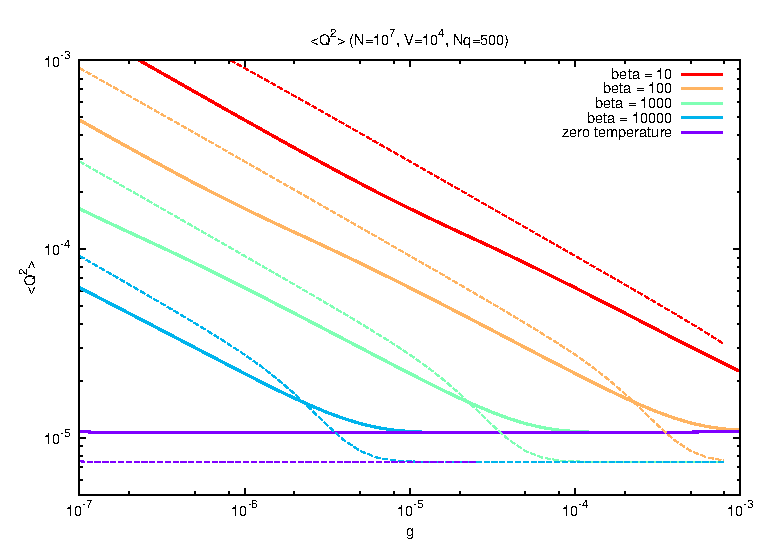
\includegraphics[width = 10cm]{./Q2.eps}
  \label{Q2}
\end{figure}
\begin{figure}[htbp]
  \centering
  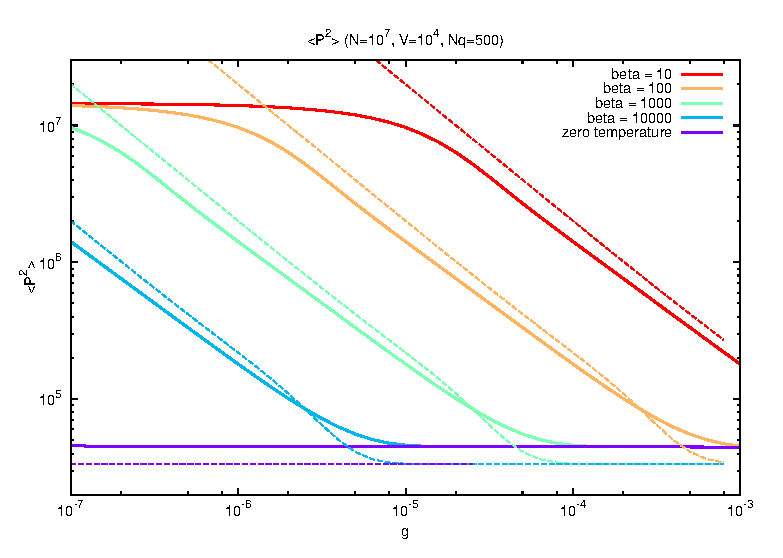
\includegraphics[width = 10cm]{./P2.eps}
  \label{P2}
\end{figure}
\\\\\\\\\\\\
図\ref{Q2},\ref{P2}\ :\ 破線は各温度に対する変分法による計算結果のプロット.$\ev{Q^2},\ev{P^2}$共に冪についてはよく一致している.

高温領域で位相ゆらぎ$\Delta Q = \sqrt{\ev{Q^2}}$,凝縮粒子数ゆらぎ$\Delta P = \sqrt{\ev{P^2}}$が増加する振る舞いは直感と一致している.
\newpage
\chapter{研究 : ゼロモードの緩和}
凝縮相と非凝縮相のcoupleを考え, 非平衡的な取り扱いを実現したい. 核生成のお話と関係がある. 位相の緩和とか見れるんじゃないかと期待. 
\section{公式}
QuantumMaster e.q.
\begin{eqnarray}
  i\dv{t}\rho_a^{nm}(t) = \sum_{n'm'}\bqty{\sum_{\mu\nu}\pqty{E_\mu - E_\nu}\Psi_{n}^{*, \mu}\Psi_{m}^{*, \nu}\Psi_{n'}^{\mu}\Psi_{m'}^{\nu}\rho_a^{n'm'}(t) + i\dpbra{nm}\hat{\calK}(t)\dpket{n'm'}\rho_a^{n'm'}(t)}
\end{eqnarray}
$A$をゼロモード演算子を含む項とする:
\begin{eqnarray}
  \dpbra{nm}A\dpket{n'm'} &=& A^{nn'}\delta_{mm'}\\
  \dpbra{nm}A^\dagger\dpket{n'm'} &=& A^{*, n'n}\delta_{mm'}\\
  \dpbra{nm}\tilde{A}\dpket{n'm'} &=& A^{*, mm'}\delta_{nn'}\\
  \dpbra{nm}\tilde{A^\dagger}\dpket{n'm'} &=& A^{m'm}\delta_{nn'}\\
\end{eqnarray}
プライム(')がつく位置に注意. これより
\begin{eqnarray}
  \dpbra{nm}\hat{A}\dpket{n'm'} &=& A^{nn'}\delta_{mm'} - A^{m'm}\delta_{nn'}\\
  \dpbra{nm}\hat{A^\dagger}\dpket{n'm'} &=& A^{*, n'n}\delta_{mm'} - A^{*, mm'}\delta_{nn'}
\end{eqnarray}
\section{具体計算 : time-convolutionless型}
もともと$\hat{\calK}(t, s),\ \dket{\rho_a(t)}$は相互作用描像のもとで定義されていたのをSchr\"odinger描像に移して計算. $s$の時間成分がexponentialの形で残ることになる.
\begin{eqnarray}
 \nonumber &&\dpbra{nm}\hat{A}_ie^{-i\hat{H}_a(t-s)}A_j^\dagger e^{i\hat{H}_a(t-s)}\dpket{n'm'}\\
  &=& \sum_{\mu\nu}\sum_{\mu'\nu'}\dpbra{nm}\hat{A}_i\dket{\mu\nu}e^{-i(E_\mu - E_\nu)(t-s)}\dbra{\mu\nu}A_j^\dagger \dket{\mu'\nu'}e^{i(E_{\mu'} - E_{\nu'})(t-s)}\dbra{\mu'\nu'}\dpket{nm}\\
  \nonumber &=& \sum_{n''m''}\sum_{\mu\nu}\sum_{\mu'\nu'}\bqty{A_i^{nn''}\delta_{mm''} - A_i^{m''m}\delta_{nn''}}A_j^{*, \mu'\mu}\delta_{\nu\nu'}\Psi_{n''}^{\mu}\Psi_{m''}^{\nu}\Psi_{n'}^{*, \mu'}\Psi_{m'}^{*, \nu'}e^{-i(E_\mu - E_\nu)(t-s)}e^{i(E_{\mu'} - E_{\nu'})(t-s)}\\
  \nonumber &=&\sum_{n''m''}\sum_{\mu\nu}\sum_{\mu'\nu'}A_i^{nn''}\delta_{mm''}A_j^{*, \mu'\mu}\delta_{\nu\nu'}\Psi_{n''}^{\mu}\Psi_{m''}^{\nu}\Psi_{n'}^{*, \mu'}\Psi_{m'}^{*, \nu'}e^{-i(E_\mu - E_\nu)(t-s)}e^{i(E_{\mu'} - E_{\nu'})(t-s)}\\
  &&- \sum_{n''m''}\sum_{\mu\nu}\sum_{\mu'\nu'}A_i^{m''m}\delta_{nn''}A_j^{*, \mu'\mu}\delta_{\nu\nu'}\Psi_{n''}^{\mu}\Psi_{m''}^{\nu}\Psi_{n'}^{*, \mu'}\Psi_{m'}^{*, \nu'}e^{-i(E_\mu - E_\nu)(t-s)}e^{i(E_{\mu'} - E_{\nu'})(t-s)}\\
  \nonumber &=&\sum_{n''}\sum_{\mu\nu}\sum_{\mu'}A_i^{nn''}A_j^{*, \mu'\mu}\Psi_{n''}^{\mu}\Psi_{m}^{\nu}\Psi_{n'}^{*, \mu'}\Psi_{m'}^{*, \nu}e^{-i(E_\mu - E_{\mu'})(t-s)}\\
  &&- \sum_{m''}\sum_{\mu\nu}\sum_{\mu'}A_i^{m''m}A_j^{*, \mu'\mu}\Psi_{n}^{\mu}\Psi_{m''}^{\nu}\Psi_{n'}^{*, \mu'}\Psi_{m'}^{*, \nu}e^{-i(E_\mu - E_{\mu'})(t-s)}\label{mid}
\end{eqnarray}
ここで$A_j^{*,\mu'\mu} = \sum_{nm}A^{*, mn}_n\Psi_n^{*, \mu}\Psi_m^{\mu'},\ \ \sum_\alpha \Psi_\beta^{*, \alpha}\Psi_{\beta'}^\alpha = \delta_{\beta\beta'}$であることを用いる:
\begin{eqnarray}
  \nonumber(\ref{mid}) &=&\sum_{n''}\sum_{\mu}\sum_{\mu'}A_i^{nn''}A_j^{*, \mu'\mu}\Psi_{n''}^{\mu}\Psi_{n'}^{*, \mu'}\delta_{mm'}e^{-i(E_\mu - E_{\mu'})(t-s)}\\
  &&- \sum_{m''}\sum_{\mu}\sum_{\mu'}A_i^{m''m}A_j^{*, \mu'\mu}\Psi_{n}^{\mu}\Psi_{n'}^{*, \mu'}\delta_{m'm''}e^{-i(E_\mu - E_{\mu'})(t-s)}\\
  \nonumber &=&\sum_{n''}\sum_{\mu}\sum_{\mu'}A_i^{nn''}A_j^{*, \mu'\mu}\Psi_{n''}^{\mu}\Psi_{n'}^{*, \mu'}\delta_{mm'}e^{-i(E_\mu - E_{\mu'})(t-s)}\\
  &&- \sum_{\mu}\sum_{\mu'}A_i^{m'm}A_j^{*, \mu'\mu}\Psi_{n}^{\mu}\Psi_{n'}^{*, \mu'}e^{-i(E_\mu - E_{\mu'})(t-s)}\\
  \nonumber &=&\sum_{n'''m'''}\sum_{n''}\sum_{\mu}\sum_{\mu'}A_i^{nn''}A_j^{*, m'''n'''}\Psi_{n'''}^{*, \mu}\Psi_{m'''}^{\mu'}\Psi_{n''}^{\mu}\Psi_{n'}^{*, \mu'}\delta_{mm'}e^{-i(E_\mu - E_{\mu'})(t-s)}\\
  &&- \sum_{n'''m'''}\sum_{\mu}\sum_{\mu'}A_i^{m'm}A_j^{*, m'''n'''}\Psi_{n'''}^{*, \mu}\Psi_{m'''}^{\mu'}\Psi_{n}^{\mu}\Psi_{n'}^{*, \mu'}e^{-i(E_\mu - E_{\mu'})(t-s)}\\
  \nonumber &=&\sum_{n'''m'''}\sum_{\mu}\sum_{\mu'}\bqty{\sum_{n''}A_i^{nn''}A_j^{*, m'''n'''}\Psi_{n''}^{\mu}\delta_{mm'}- A_i^{m'm}A_j^{*, m'''n'''}\Psi_{n}^{\mu}}\Psi_{n'''}^{*, \mu}\Psi_{m'''}^{\mu'}\Psi_{n'}^{*, \mu'}e^{-i(E_\mu - E_{\mu'})(t-s)}\label{end1}\\
\end{eqnarray}
同様に$\hat{\calK}$に必要な項を計算していく.
\begin{comment}
  以下では(\ref{end1})と添字が異なる部分に下線を引いている.
\end{comment}
\begin{eqnarray}
 \nonumber &&\dpbra{nm}\hat{A^\dagger}_ie^{-i\hat{H}_a(t-s)}\tilde{A}_j^\dagger e^{i\hat{H}_a(t-s)}\dpket{n'm'}\\
  %&=& \sum_{\mu\nu}\sum_{\mu'\nu'}\dpbra{nm}\hat{A^\dagger}_i\dket{\mu\nu}e^{-i(E_\mu - E_\nu)(t-s)}\dbra{\mu\nu}\tilde{A}_j^\dagger \dket{\mu'\nu'}e^{i(E_{\mu'} - E_{\nu'})(t-s)}\dbra{\mu'\nu'}\dpket{nm}\\
  \nonumber &=& \sum_{n''m''}\sum_{\mu\nu}\sum_{\mu'\nu'}\bqty{A_i^{*,  {n''n}}\delta_{mm''} - A_i^{*,  {mm''}}\delta_{nn''}}A_j^{ {\nu'\nu}}\delta_{ {\mu\mu'}}\Psi_{n''}^{\mu}\Psi_{m''}^{\nu}\Psi_{n'}^{*, \mu'}\Psi_{m'}^{*, \nu'}e^{-i(E_\mu - E_\nu)(t-s)}e^{i(E_{\mu'} - E_{\nu'})(t-s)}\\
  \nonumber &=&\sum_{n''m''}\sum_{\mu\nu}\sum_{\mu'\nu'}A_i^{*,  {n''n}}\delta_{mm''}A_j^{ {\nu'\nu}}\delta_{ {\mu\mu'}}\Psi_{n''}^{\mu}\Psi_{m''}^{\nu}\Psi_{n'}^{*, \mu'}\Psi_{m'}^{*, \nu'}e^{-i(E_\mu - E_\nu)(t-s)}e^{i(E_{\mu'} - E_{\nu'})(t-s)}\\
  &&- \sum_{n''m''}\sum_{\mu\nu}\sum_{\mu'\nu'}A_i^{*,  {mm''}}\delta_{nn''}A_j^{ {\nu'\nu}}\delta_{ {\mu\mu'}}\Psi_{n''}^{\mu}\Psi_{m''}^{\nu}\Psi_{n'}^{*, \mu'}\Psi_{m'}^{*, \nu'}e^{-i(E_\mu - E_\nu)(t-s)}e^{i(E_{\mu'} - E_{\nu'})(t-s)}\\
  \nonumber &=&\sum_{n''}\sum_{\mu\nu}\sum_{ {\nu'}}A_i^{*,  {n''n}}A_j^{ {\nu'\nu}}\Psi_{n''}^{\mu}\Psi_{m}^{\nu}\Psi_{n'}^{*, \mu}\Psi_{m'}^{*, \nu'}e^{ {i(E_\nu- E_{\nu'})(t-s)}}\\
  &&- \sum_{m''}\sum_{\mu\nu}\sum_{ {\nu'}}A_i^{*,  {mm''}}A_j^{ {\nu'\nu}}\Psi_{n}^{\mu}\Psi_{m''}^{\nu}\Psi_{n'}^{*, \mu}\Psi_{m'}^{*, \nu'}e^{ {i(E_\nu- E_{\nu'})(t-s)}}\\
  %\nonumber &=&\sum_{n''}\sum_{ {\nu}}\sum_{ {\nu'}}A_i^{*,  {n''n}}A_j^{ {\nu'\nu}}\Psi_{m}^{\nu}\Psi_{m'}^{*, \nu'}\delta_{ {n'n''}}e^{ {i(E_\nu- E_{\nu'})(t-s)}}\\
  %&&- \sum_{m''}\sum_{ {\nu}}\sum_{ {\nu'}}A_i^{*,  {mm''}}A_j^{ {\nu'\nu}}\Psi_{m''}^{\nu}\Psi_{m'}^{*, \nu'}\delta_{ {nn'}}e^{ {i(E_\nu- E_{\nu'})(t-s)}}\\
  \nonumber &=&\sum_{ {\nu}}\sum_{ {\nu'}}A_i^{*,  {n'n}}A_j^{ {\nu'\nu}}\Psi_{m}^{\nu}\Psi_{m'}^{*, \nu'}e^{ {i(E_\nu- E_{\nu'})(t-s)}}\\
  &&- \sum_{ {m''}}\sum_{ {\nu}}\sum_{ {\nu'}}A_i^{*,  {mm''}}A_j^{ {\nu'\nu}}\Psi_{m''}^{\nu}\Psi_{m'}^{*, \nu'}\delta_{ {nn'}}e^{ {i(E_\nu- E_{\nu'})(t-s)}}\\
  \nonumber &=&\sum_{n'''m'''}\sum_{ {\nu}}\sum_{ {\nu'}}A_i^{*, {n'n}}A_j^{{n'''m'''}}\Psi_{n'''}^{ {*, \nu'}}\Psi_{m'''}^{ {\nu}}\Psi_{m}^{ {\nu}}\Psi_{m'}^{*, \nu'}e^{ {i(E_\nu- E_{\nu'})(t-s)}}\\
  &&- \sum_{n'''m'''}\sum_{ {m''}}\sum_{ {\nu}}\sum_{ {\nu'}}A_i^{*,  {mm''}}A_j^{ {n'''m'''}}\Psi_{n'''}^{ {*, \nu'}}\Psi_{m'''}^{ {\nu}}\Psi_{m''}^{\nu}\Psi_{m'}^{*, \nu'}\delta_{ {nn'}}e^{ {i(E_\nu- E_{\nu'})(t-s)}}\\
  \nonumber &=&\sum_{n'''m'''}\sum_{\nu}\sum_{\nu'}\bqty{A_i^{*, n'n}A_j^{n'''m'''}\Psi_{m}^{\nu} - \sum_{m''}A_i^{*, mm''}A_j^{n'''m'''}\Psi_{m''}^{\nu}\delta_{nn'}}\Psi_{n'''}^{*, \nu'}\Psi_{m'''}^{\nu}\Psi_{m'}^{*, \nu'}e^{i(E_\nu- E_{\nu'})(t-s)}\\
\end{eqnarray}

\begin{eqnarray}
\nonumber  &&\dpbra{nm}\hat{A}_ie^{-i\hat{H}_a(t-s)}\tilde{A}_j e^{i\hat{H}_a(t-s)}\dpket{n'm'}\\
  \nonumber &=& \sum_{n''m''}\sum_{\mu\nu}\sum_{\mu'\nu'}\bqty{A_i^{ {nn''}}\delta_{mm''} - A_i^{ {m''m}}\delta_{nn''}}A_j^{ {*, \nu'\nu}}\delta_{ {\mu\mu'}}\Psi_{n''}^{\mu}\Psi_{m''}^{\nu}\Psi_{n'}^{*, \mu'}\Psi_{m'}^{*, \nu'}e^{-i(E_\mu - E_\nu)(t-s)}e^{i(E_{\mu'} - E_{\nu'})(t-s)}\\
  \nonumber &=&\sum_{n''}\sum_{\mu\nu}\sum_{ {\nu'}}A_i^{nn''}A_j^{*, \nu'\nu}\Psi_{n''}^{\mu}\Psi_{m}^{\nu}\Psi_{n'}^{*, \mu}\Psi_{m'}^{*, \nu'}e^{ {i(E_\nu- E_{\nu'})(t-s)}}\\
  &&- \sum_{m''}\sum_{\mu\nu}\sum_{ {\nu'}}A_i^{m''m}A_j^{ {*, \nu'\nu}}\Psi_{n}^{\mu}\Psi_{m''}^{\nu}\Psi_{n'}^{*, \mu}\Psi_{m'}^{*, \nu'}e^{ {i(E_\nu- E_{\nu'})(t-s)}}\\
  \nonumber &=&\sum_{n''}\sum_{ {\nu}}\sum_{ {\nu'}}A_i^{ {nn''}}A_j^{*, \nu'\nu}\Psi_{m}^{\nu}\Psi_{m'}^{*, \nu'}\delta_{ {n'n''}}e^{ {i(E_\nu- E_{\nu'})(t-s)}}\\
  &&- \sum_{m''}\sum_{ {\nu}}\sum_{ {\nu'}}A_i^{m''m}A_j^{*, \nu'\nu}\Psi_{m''}^{\nu}\Psi_{m'}^{*, \nu'}\delta_{ {nn'}}e^{ {i(E_\nu- E_{\nu'})(t-s)}}\\
%  \nonumber &=&\sum_{ {\nu}}\sum_{ {\nu'}}A_i^{nn'}A_j^{*, \nu'\nu}\Psi_{m}^{\nu}\Psi_{m'}^{*, \nu'}e^{ {i(E_\nu- E_{\nu'})(t-s)}}\\
 % &&- \sum_{ {m''}}\sum_{ {\nu}}\sum_{ {\nu'}}A_i^{m''m}A_j^{*, \nu'\nu}\Psi_{m''}^{\nu}\Psi_{m'}^{*, \nu'}\delta_{ {nn'}}e^{ {i(E_\nu- E_{\nu'})(t-s)}}\\
  \nonumber &=&\sum_{n'''m'''}\sum_{ {\nu}}\sum_{ {\nu'}}A_i^{nn'}A_j^{*, m'''n'''}\Psi_{n'''}^{ {*, \nu'}}\Psi_{m'''}^{ {\nu}}\Psi_{m}^{ {\nu}}\Psi_{m'}^{*, \nu'}e^{ {i(E_\nu- E_{\nu'})(t-s)}}\\
  &&- \sum_{n'''m'''}\sum_{ {m''}}\sum_{ {\nu}}\sum_{ {\nu'}}A_i^{m''m}A_j^{*, m'''n'''}\Psi_{n'''}^{ {*, \nu'}}\Psi_{m'''}^{ {\nu}}\Psi_{m''}^{\nu}\Psi_{m'}^{*, \nu'}\delta_{ {nn'}}e^{ {i(E_\nu- E_{\nu'})(t-s)}}\\
  \nonumber &=&\sum_{n'''m'''}\sum_{\nu}\sum_{\nu'}\bqty{A_i^{nn'}A_j^{*, m'''n'''}\Psi_{m}^{\nu}- \sum_{m''}A_i^{m''m}A_j^{*, m'''n'''}\Psi_{m''}^{\nu}\delta_{nn'} }\Psi_{n'''}^{*, \nu'}\Psi_{m'''}^{\nu}\Psi_{m'}^{*, \nu'}e^{i(E_\nu- E_{\nu'})(t-s)}\\
\end{eqnarray}
\begin{eqnarray}
\nonumber  &&\dpbra{nm}\hat{A^\dagger}_ie^{-i\hat{H}_a(t-s)}A_j e^{i\hat{H}_a(t-s)}\dpket{n'm'}\\
  \nonumber &=& \sum_{n''m''}\sum_{\mu\nu}\sum_{\mu'\nu'}\bqty{A_i^{*, n''n}\delta_{mm''} - A_i^{*, mm''}\delta_{nn''}}A_j^{ {\mu\mu'}}\delta_{ {\nu\nu'}}\Psi_{n''}^{\mu}\Psi_{m''}^{\nu}\Psi_{n'}^{*, \mu'}\Psi_{m'}^{*, \nu'}e^{-i(E_\mu - E_\nu)(t-s)}e^{i(E_{\mu'} - E_{\nu'})(t-s)}\\
  \nonumber &=&\sum_{n''}\sum_{\mu\nu}\sum_{ {\mu'}}A_i^{*, n''n}A_j^{\mu\mu'}\Psi_{n''}^{\mu}\Psi_{m}^{\nu}\Psi_{n'}^{*, \mu'}\Psi_{m'}^{*, \nu}e^{ {-i(E_\mu- E_{\mu'})(t-s)}}\\
  &&- \sum_{m''}\sum_{\mu\nu}\sum_{ {\mu'}}A_i^{*, mm''}A_j^{\mu\mu'}\Psi_{n}^{\mu}\Psi_{m''}^{\nu}\Psi_{n'}^{*, \mu'}\Psi_{m'}^{*, \nu}e^{ {-i(E_\mu- E_{\mu'})(t-s)}}\\
  \nonumber &=&\sum_{n''}\sum_{ {\mu}}\sum_{ {\mu'}}A_i^{ {*, n''n}}A_j^{\mu\mu'}\Psi_{n''}^{\mu}\Psi_{n'}^{*, \mu'}\delta_{mm'}e^{ {-i(E_\mu- E_{\mu'})(t-s)}}\\
  &&- \sum_{m''}\sum_{ {\mu}}\sum_{ {\mu'}}A_i^{*, mm''}A_j^{\mu\mu'}\Psi_{n}^{\mu}\Psi_{n'}^{*, \mu'}\delta_{m'm''}e^{ {-i(E_\mu- E_{\mu'})(t-s)}}\\
  \nonumber &=&\sum_{n'''m'''}\sum_{n''}\sum_{ {\mu}}\sum_{ {\mu'}}A_i^{ {*, n''n}}A_j^{n'''m'''}\Psi_{n'''}^{*, \mu}\Psi_{m'''}^{\mu'}\Psi_{n''}^{\mu}\Psi_{n'}^{*, \mu'}\delta_{mm'}e^{ {-i(E_\mu- E_{\mu'})(t-s)}}\\
  &&- \sum_{n'''m'''}\sum_{ {\mu}}\sum_{ {\mu'}}A_i^{*, mm'}A_j^{n'''m'''}\Psi_{n'''}^{*, \mu}\Psi_{m'''}^{\mu'}\Psi_{n}^{\mu}\Psi_{n'}^{*, \mu'}e^{ {-i(E_\mu- E_{\mu'})(t-s)}}\\
    \nonumber &=&\sum_{n'''m'''}\sum_{ {\mu}}\sum_{ {\mu'}}\bqty{\sum_{n''}A_i^{ {*, n''n}}A_j^{n'''m'''}\Psi_{n''}^{\mu}\delta_{mm'} - A_i^{*, mm'}A_j^{n'''m'''}\Psi_{n}^{\mu}}\Psi_{n'''}^{*, \mu}\Psi_{m'''}^{\mu'}\Psi_{n'}^{*, \mu'}e^{ {-i(E_\mu- E_{\mu'})(t-s)}}\\
\end{eqnarray}
まとめると,
\begin{screen}
  \begin{eqnarray}
\nonumber    &&\dpbra{nm}\hat{A}_ie^{-i\hat{H}_a(t-s)}A_j^\dagger e^{i\hat{H}_a(t-s)}\dpket{n'm'}\\
\nonumber    &=&\sum_{n'''m'''}\sum_{\mu}\sum_{\mu'}\bqty{\sum_{n''}A_i^{nn''}A_j^{*, m'''n'''}\Psi_{n''}^{\mu}\delta_{mm'}- A_i^{m'm}A_j^{*, m'''n'''}\Psi_{n}^{\mu}}\Psi_{n'''}^{*, \mu}\Psi_{m'''}^{\mu'}\Psi_{n'}^{*, \mu'}e^{-i(E_\mu - E_{\mu'})(t-s)}\\\\
    \nonumber &&\dpbra{nm}\hat{A^\dagger}_ie^{-i\hat{H}_a(t-s)}\tilde{A}_j^\dagger e^{i\hat{H}_a(t-s)}\dpket{n'm'}\\
\nonumber    &=&\sum_{n'''m'''}\sum_{\nu}\sum_{\nu'}\bqty{A_i^{*, n'n}A_j^{n'''m'''}\Psi_{m}^{\nu}- \sum_{m''}A_i^{*, mm''}A_j^{n'''m'''}\Psi_{m''}^{\nu}\delta_{nn'}}\Psi_{n'''}^{*, \nu'}\Psi_{m'''}^{\nu}\Psi_{m'}^{*, \nu'}e^{i(E_\nu- E_{\nu'})(t-s)}\\\\
    \nonumber&&\dpbra{nm}\hat{A}_ie^{-i\hat{H}_a(t-s)}\tilde{A}_j e^{i\hat{H}_a(t-s)}\dpket{n'm'}\\
\nonumber    &=&\sum_{n'''m'''}\sum_{\nu}\sum_{\nu'}\bqty{A_i^{nn'}A_j^{*, m'''n'''}\Psi_{m}^{\nu}- \sum_{m''}A_i^{m''m}A_j^{*, m'''n'''}\Psi_{m''}^{\nu}\delta_{nn'} }\Psi_{n'''}^{*, \nu'}\Psi_{m'''}^{\nu}\Psi_{m'}^{*, \nu'}e^{i(E_\nu- E_{\nu'})(t-s)}\\\\
\nonumber    &&\dpbra{nm}\hat{A^\dagger}_ie^{-i\hat{H}_a(t-s)}A_j e^{i\hat{H}_a(t-s)}\dpket{n'm'}\\
    \nonumber &=&\sum_{n'''m'''}\sum_{ {\mu}}\sum_{ {\mu'}}\bqty{\sum_{n''}A_i^{ {*, n''n}}A_j^{n'''m'''}\Psi_{n''}^{\mu}\delta_{mm'} - A_i^{*, mm'}A_j^{n'''m'''}\Psi_{n}^{\mu}}\Psi_{n'''}^{*, \mu}\Psi_{m'''}^{\mu'}\Psi_{n'}^{*, \mu'}e^{ {-i(E_\mu- E_{\mu'})(t-s)}}\\
  \end{eqnarray}
\end{screen}
\textbf{添字が合ってるかとっても心配.}

\section{具体計算 : 摂動項$\calK(t)$}
我々が計算したいのは
\begin{eqnarray}
  \calK(t) &=& \calK_1(t) + \calK_2(t)\\
\nonumber  \calK_1(t)&=& -\frac{2Vg^2}{(2\pi)^6}\int_{t_0}^tds\int d\bm{k}_1d\bm{k}_2d\bm{k}_3\delta(\bm{k}_1+\bm{k}_2-\bm{k}_3)\\
  \nonumber  &&\times\Bigl[n_{k_1}n_{k_2}(1+n_{k_3})\Bqty{ e^{i(\omega_{k_1}+\omega_{k_2}  - \omega_{k_3})(t-s)}\hat{A}_1(t)A_1^\dagger(s) - e^{-i(\omega_{k_1}+\omega_{k_2}  - \omega_{k_3})(t-s)}\hat{A}^\dagger_1(t)\tilde{A}_1^\dagger(s) }\\
    \nonumber  &&-(1+n_{k_1})(1+n_{k_2})n_{k_3}\Bqty{e^{i(\omega_{k_1}+\omega_{k_2}  - \omega_{k_3})(t-s)}\hat{A}_1(t)\tilde{A}_1(s) - e^{-i(\omega_{k_1}+\omega_{k_2}  - \omega_{k_3})(t-s)}\hat{A}^\dagger_1(t)A_1(s) }\Bigr]\\
  \\
  \nonumber  \calK_2(t) &=& -\frac{Vg^2}{2(2\pi)^6}\int_{t_0}^tds\int d\bm{k}\Bigl[ n_k^2\Bqty{e^{2i\omega_{k}(t-s)}\hat{A}_2(t)A_2^\dagger(s) - e^{-2i\omega_{k}(t-s)}\hat{A}^\dagger_2(t)\tilde{A}_2^\dagger(s)}\\
    &&-(1+n_{k})^2\Bqty{e^{2i\omega_{k}(t-s)}\hat{A}_2(t)\tilde{A}_2(s) - e^{-2i\omega_{k}(t-s)}\hat{A}^\dagger_2(t)A_2(s)}\Bigr]
\end{eqnarray}
だが, 演算子は全て相互作用描像である. これをSchr\"odinger描像に移して計算するので, $A(s)\rightarrow e^{-i\hat{H}_a(t-s)}Ae^{i\hat{H}_a(t-s)}$として期待値を取る. Schr\"odinger描像に移した期待値の公式は既に上で導出した.

さらにQuantum Master e.q.をマルコフ近似すると$\dket{\rho_a(s)}\rightarrow\dket{\rho_a(t)}$かつ$t_0\rightarrow -\infty$とすればよい. $s$積分は
\begin{eqnarray}
  \int_{-\infty}^t ds e^{iW(t-s)} \simeq \pi\delta(W)
\end{eqnarray}
\underline{のように計算できる(主値を捨てている)}ことから, $\dpbra{nm}\calK_2(t)\dpket{n'm'}$は
\begin{eqnarray}
  &&\dpbra{nm}\calK_2(t)\dpket{n'm'} = -\frac{Vg^2}{2(2\pi)^6}\int d\bm{k}\\
  \nonumber  &&\times\sum_{n'''m'''}\Bigl[ n_k^2\Bqty{\sum_{n''}A_2^{nn''}A_2^{*, m'''n'''}\delta_{mm'}M_{n'''n''}M_{n'm'''}' - A_2^{m'm}A_2^{*, m'''n'''}M_{n'''n}M_{n'm'''}'}\delta(2\omega_k - E_\mu + E_{\mu'})\\
    \nonumber &&\ \ + n_k^2\Bqty{A_2^{*, n'n}A_2^{n'''m'''}N_{mm'''}N_{n'''m'}' - \sum_{m''}A_2^{*, mm''}A_2^{n'''m'''}\delta_{nn'}N_{m''m'''}N_{n'''m'}'}\delta(-2\omega_k + E_\nu - E_{\nu'})\\
    \nonumber &&- (1 + n_k)^2\Bqty{A_2^{nn'}A_2^{*, m'''n'''}N_{mm'''}N_{n'''m'}' - \sum_{m''}A_2^{m''m}A_2^{*, m'''n'''}\delta_{nn'}N_{m''m'''}N_{n'''m'}'}\delta(2\omega_k + E_\nu - E_{\nu'})\\
   \nonumber&&-(1+n_k)^2\Bqty{\sum_{n''}A_2^{*, n''n}A_2^{n'''m'''}\delta_{mm'}M_{n'''n''}M_{n'm'''}' - A_2^{*, mm'}A_2^{n'''m'''}M_{n'''n}M_{n'm'''}'}\delta(-2\omega_k - E_\mu + E_{\mu'})\Bigr]\\
\end{eqnarray}
ここで
\begin{eqnarray}
  M_{\alpha\beta} &\equiv& \sum_\mu \Psi_\alpha^{*, \mu}\Psi_\beta^{\mu}\hspace{0.5cm}M_{\alpha\beta}' \equiv \sum_{\mu'} \Psi_\alpha^{*, \mu'}\Psi_\beta^{\mu'}\\
    N_{\alpha\beta} &\equiv& \sum_\nu \Psi_\alpha^{\nu}\Psi_\beta^{\nu}\hspace{0.5cm}N_{\alpha\beta}' \equiv \sum_{\nu'} \Psi_\alpha^{*, \nu'}\Psi_\beta^{*, \nu'}
\end{eqnarray}
としている. さらに$\bm{k}$積分を実行する. ここで
\begin{eqnarray}
  \int d\bm{k} n_k^2\delta(2\omega_k - E) &=& \int_0^\infty dk\int_0^\pi d\theta \int_0^{2\pi}d\phi k\sin{\theta}n_k^2\delta(k^2 - E) \\
  &=& \int_0^\pi d\theta \int_0^{2\pi}d\phi \sqrt{E}\theta(E)\sin{\theta}n_k^2\\
  &=& 4\pi\sqrt{E}\theta(E)n_E^2
\end{eqnarray}
であることから
\begin{eqnarray}
  R_2(E) \equiv \frac{Vg^2}{8\pi}\theta(E)n_E^2\sqrt{E}\hspace{0.5cm}R_2'(E) \equiv \frac{Vg^2}{8\pi}\theta(E)(1 + n_E)^2\sqrt{E}
\end{eqnarray}
とする. スターの位置に注意. ここで$\theta(E)$は階段関数. これを用いると
\begin{eqnarray}
  \nonumber &&\dpbra{nm}\calK_2(t)\dpket{n'm'} =\\
  \nonumber &&\sum_{n'''m'''}\Bigl[-\Bqty{\sum_{n''}A_2^{nn''}A_2^{*, m'''n'''}\delta_{mm'}M_{n'''n''}M_{n'm'''}' - A_2^{m'm}A_2^{*, m'''n'''}M_{n'''n}M_{n'm'''}'}R_2(E_\mu - E_{\mu'})\\
    \nonumber &&- \Bqty{A_2^{*, n'n}A_2^{n'''m'''}N_{mm'''}N_{n'''m'}' - \sum_{m''}A_2^{*, mm''}A_2^{n'''m'''}\delta_{nn'}N_{m''m'''}N_{n'''m'}'}R_2(E_\nu - E_{\nu'})\\
    \nonumber &&+ \Bqty{A_2^{nn'}A_2^{*, m'''n'''}N_{mm'''}N_{n'''m'}' - \sum_{m''}A_2^{m''m}A_2^{*, m'''n'''}\delta_{nn'}N_{m''m'''}N_{n'''m'}'}R_2'(-E_\nu + E_{\nu'})\\
   \nonumber&&+\Bqty{\sum_{n''}A_2^{*, n''n}A_2^{n'''m'''}\delta_{mm'}M_{n'''n''}M_{n'm'''}' - A_2^{*, mm'}A_2^{n'''m'''}M_{n'''n}M_{n'm'''}'}R_2'(- E_\mu + E_{\mu'})\Bigr]\\\label{K1}
\end{eqnarray}
\textbf{符号が合ってるかどうかとても心配.}

さらに$\dpbra{nm}\calK_1(t)\dpket{n'm'}$を計算する前に\underline{積分公式を導出しておく}:
\begin{eqnarray}
  I(E) &=& \int d\bm{k}_1d\bm{k}_2d\bm{k}_3\delta(\bm{k}_1+\bm{k}_2-\bm{k}_3)\delta(\omega_{k_1} + \omega_{k_2} - \omega_{k_3} + E)a(\omega_{k_1})b(\omega_{k_2})c(\omega_{k_3})\\
  &=& 8\pi^2\int_0^\infty d\omega_1\int_{\frac{E_2}{4\omega_1}}^\infty d\omega_2 a(\omega_1)b(\omega_2)c(\omega_1 + \omega_2 + E)
\end{eqnarray}
となる. これ以上は$a, b, c$の具体形が必要. これを用いると(\ref{K1})の添字を$2\rightarrow1$にしたものと同様. ただし:
\begin{eqnarray}
  R_1(E) &=& \frac{Vg^2}{4\pi^3}\int_0^\infty d\omega_1\int_{\frac{E^2}{4\omega_1}}^\infty d\omega_2 n_{\omega_1}n_{\omega_2}(1 + n_{\omega_1 + \omega_2 + E})\\
  R_1'(E) &=& \frac{Vg^2}{4\pi^3}\int_0^\infty d\omega_1\int_{\frac{E^2}{4\omega_1}}^\infty d\omega_2 (1 + n_{\omega_1})(1 + n_{\omega_2})n_{\omega_1 + \omega_2 + E}
\end{eqnarray}
とする. つまり解くべき方程式は
\begin{eqnarray}
  i\dv{t}\rho_a^{nm}(t) &=& \sum_{n'm'}\bqty{\sum_{\mu\nu}\pqty{E_\mu - E_\nu}\Psi_{n}^{*, \mu}\Psi_{m}^{*, \nu}\Psi_{n'}^{\mu}\Psi_{m'}^{\nu} + i\dpbra{nm}\hat{\calK}(t)\dpket{n'm'}}\rho_a^{n'm'}(t)\\
  &\equiv& \sum_{n'm'} L^{nm, n'm'}\rho_a^{n'm'}(t)\label{Master2}
\end{eqnarray}
である. ただし
\begin{eqnarray}
  &&L^{nm, n'm'} = \sum_{\mu\nu}\pqty{E_\mu - E_\nu}\Psi_{n}^{*, \mu}\Psi_{m}^{*, \nu}\Psi_{n'}^{\mu}\Psi_{m'}^{\nu} \\
  &&+\sum_{i = 1, 2}\sum_{n'''m'''}\Bigl[\nonumber -\Bqty{\sum_{n''}A_i^{nn''}A_i^{*, m'''n'''}\delta_{mm'}M_{n'''n''}M_{n'm'''}' - A_i^{m'm}A_i^{*, m'''n'''}M_{n'''n}M_{n'm'''}'}R_i(E_\mu - E_{\mu'})\\
    \nonumber &&- \Bqty{A_i^{*, n'n}A_i^{n'''m'''}N_{mm'''}N_{n'''m'}' - \sum_{m''}A_i^{*, mm''}A_i^{n'''m'''}\delta_{nn'}N_{m''m'''}N_{n'''m'}'}R_i(E_\nu - E_{\nu'})\\
    \nonumber &&+ \Bqty{A_i^{nn'}A_i^{*, m'''n'''}N_{mm'''}N_{n'''m'}' - \sum_{m''}A_i^{m''m}A_i^{*, m'''n'''}\delta_{nn'}N_{m''m'''}N_{n'''m'}'}R_i'(-E_\nu + E_{\nu'})\\
   \nonumber&&+\Bqty{\sum_{n''}A_i^{*, n''n}A_i^{n'''m'''}\delta_{mm'}M_{n'''n''}M_{n'm'''}' - A_i^{*, mm'}A_i^{n'''m'''}M_{n'''n}M_{n'm'''}'}R_i'(- E_\mu + E_{\mu'})\Bigr]\\\label{L}
\end{eqnarray}
\section{数値計算へ向けて}
期待値の計算のためにQuantum Master e.q.(\ref{Master2})を解いて密度行列$\rho_a$を得るのがひとまずの目的. これが得られればいろんな物理量の計算ができる. (\ref{Master2})のエッセンスは$L^{nm, n'm'}$にある. $L^{nm, n'm'}$を数値計算においてどのように表現するかをまとめる.
\subsection{$E_\mu\cdot E_\nu$}
$\ket{\mu},\ \ket{\nu}$は$H_a$のエネルギー固有状態として定義されている:
\begin{eqnarray}
  H_a\ket{\mu} = E_\mu\ket{\mu},\hspace{0.5cm}\tilde{H}_a\ket{\nu} = E_\nu\ket{\nu}
\end{eqnarray}
$\ket{\nu}$はチルダハミルトニアンの固有状態というだけで, 実質ノンチルダとモノに変わりはない. ということで, これを$\varphi_{\rm ex},\ \varphi_{\rm ex}^\dagger$の粒子数状態で行列表示する:
\begin{eqnarray}
  \sum_m\pbra{n}H_a\pket{m}(m\ket{\mu} &=& E_\mu(n\ket{\mu}\\
\Longleftrightarrow  \sum_m\pbra{n}H_a\pket{m}\Psi_m^\mu &=& E_\mu\Psi_n^\mu
\end{eqnarray}
これをLapackで解けば$\Psi, E$のセットが得られる.
\subsection{$A_i^{nm}$}
$i = 1, 2$のみなので具体的に計算してみる:
\begin{eqnarray}
  A_1^{nm} &=& \pbra{n}A_1\pket{m} = \pbra{n}\varphi_0\pket{m} = \sqrt{m}(n|m-1) = \sqrt{m}\delta_{n, m-1}\\
  A_2^{nm} &=& \pbra{n}A_2\pket{m} = \pbra{n}\varphi_0^2\pket{m} = \sqrt{m(m-1)}(n|m-2) = \sqrt{m(m-1)}\delta_{n, m-2}\\
  A_2^{*, nm} &=& \pqty{A_2^{nm}}^* = A_2^{nm}
\end{eqnarray}
とても簡単になる.
\subsection{$N_{nm}\cdot N_{nm}'$}
\begin{eqnarray}
  N_{nm} = \sum_\nu\Psi_n^\nu\Psi_m^\nu
\end{eqnarray}
なので$\Psi$のセットがあれば自明.
\subsection{$R_i$}
$R_1, R_2$共に$n_k$が必要. $n_k$の定義は
\begin{eqnarray}
  n_k\delta(\bm{k} - \bm{k}') = \ev{b_{\bm{k}}b_{\bm{k}}^\dagger}
\end{eqnarray}
であり, $H_R$は$\varphi_{\rm ex}$の2次なので対角化可能. 系の時間発展に対して変化が少ない過程をしているので熱平衡状態にあると考えて良い:
\begin{eqnarray}
  n_k = \frac{1}{e^{\beta\omega_k'}-1}\delta(\bm{k} - \bm{k}')
\end{eqnarray}
一様系では
\begin{eqnarray}
  \omega_k' = \sqrt{\frac{\hbar^2k^2}{2m}\pqty{\frac{\hbar^2k^2}{2m} + 2gn_0}}
\end{eqnarray}
であることを利用して
\begin{eqnarray}
 && n_E = \frac{1}{e^{\beta\omega_E'}-1}\hspace{0.5cm}\omega_E' = \sqrt{\frac{\hbar^2E}{2m}\pqty{\frac{\hbar^2E}{2m} + 2gn_0}}\\
  &&n_{\omega_1 + \omega_2 + E} = \frac{1}{e^{\beta\omega'}-1}\hspace{0.5cm}\omega' = \sqrt{\frac{\hbar^2(\frac{\omega_1 + \omega_2}{2}+E)}{2m}\pqty{\frac{\hbar^2(\frac{\omega_1 + \omega_2}{2}+E)}{2m} + 2gn_0}}
\end{eqnarray}
とすることができる. また$\xi^2 = n_0$より$n_0$はTDGP方程式により決定される. つまり, $\xi$の時間発展は密度行列の時間発展とは別の枠組みで与えられていることになる. TDGPに量子補正を加えるべきかどうかはわからない. 量子補正を入れると自己無撞着の計算がとてもめんどくさくなる. 今のところ, ゼロモードはDepletionに影響を与えない(比熱は影響を受ける)という結論なので, 補正無しのTDGPでもよい気がする.

ちなみに今回は$\xi$は時間発展しないものとしているのであしからず. 
\section{$L^{nm,n'm'}$の整理}
以上の結論から$L^{nm,n'm'}$を整理する. (\ref{L})の第二項の和を$i = 1, 2$それぞれついて計算する.

i = 1について:
\begin{eqnarray}
  &&\sum_{n'''m'''}\Bigl[\nonumber -\Bqty{\sum_{n''}A_1^{nn''}A_1^{*, m'''n'''}\delta_{mm'}M_{n'''n''}M_{n'm'''}' - A_1^{m'm}A_1^{*, m'''n'''}M_{n'''n}M_{n'm'''}'}R_1(E_\mu - E_{\mu'})\\
    \nonumber &&- \Bqty{A_1^{*, n'n}A_1^{n'''m'''}N_{mm'''}N_{n'''m'}' - \sum_{m''}A_1^{*, mm''}A_1^{n'''m'''}\delta_{nn'}N_{m''m'''}N_{n'''m'}'}R_1(E_\nu - E_{\nu'})\\
    \nonumber &&+ \Bqty{A_1^{nn'}A_1^{*, m'''n'''}N_{mm'''}N_{n'''m'}' - \sum_{m''}A_1^{m''m}A_1^{*, m'''n'''}\delta_{nn'}N_{m''m'''}N_{n'''m'}'}R_1'(-E_\nu + E_{\nu'})\\
    \nonumber&&+\Bqty{\sum_{n''}A_1^{*, n''n}A_1^{n'''m'''}\delta_{mm'}M_{n'''n''}M_{n'm'''}' - A_1^{*, mm'}A_1^{n'''m'''}M_{n'''n}M_{n'm'''}'}R_1'(- E_\mu + E_{\mu'})\Bigr]\\
  \\
  &=&\sum_{n'''m'''}\Bigl[\nonumber -\Bqty{\sum_{n''}\sqrt{n''}\delta_{n, n''-1}\sqrt{n'''}\delta_{m''', n'''-1}\delta_{mm'}M_{n'''n''}M_{n'm'''}' - \sqrt{m}\delta_{m', m-1}\sqrt{n'''}\delta_{m''', n'''-1}M_{n'''n}M_{n'm'''}'}\\
    \nonumber&&\hspace{14cm}\times R_1(E_\mu - E_{\mu'})\\
    \nonumber &&- \Bqty{\sqrt{n}\delta_{n', n-1}\sqrt{m'''}\delta_{n''', m'''-1}N_{mm'''}N_{n'''m'}' - \sum_{m''}\sqrt{m''}\delta_{m, m''-1}\sqrt{m'''}\delta_{n''', m'''-1}\delta_{nn'}N_{m''m'''}N_{n'''m'}'}\\
    \nonumber&&\hspace{14cm}\times R_1(E_\nu - E_{\nu'})\\
    \nonumber &&+ \Bqty{\sqrt{n'}\delta_{n, n'-1}\sqrt{n'''}\delta_{m''', n'''-1}N_{mm'''}N_{n'''m'}' - \sum_{m''}\sqrt{m}\delta_{m'', m-1}\sqrt{n'''}\delta_{m''', n'''-1}\delta_{nn'}N_{m''m'''}N_{n'''m'}'}\\
    \nonumber&&\hspace{14cm}\times R_1'(-E_\nu + E_{\nu'})\\
    \nonumber&&+\Bqty{\sum_{n''}\sqrt{n}\delta_{n'', n-1}\sqrt{m'''}\delta_{n''', m'''-1}\delta_{mm'}M_{n'''n''}M_{n'm'''}' - \sqrt{m'}\delta_{m, m'-1}\sqrt{m'''}\delta_{n''', m'''-1}M_{n'''n}M_{n'm'''}'}\\
    \nonumber&&\hspace{14cm}\times R_1'(- E_\mu + E_{\mu'})\Bigr]\\
  \\
  &=&\sum_{\ell }\Bigl[\nonumber -\sum_{\mu\mu'}\Bqty{ \sqrt{n+1}\sqrt{\ell }\delta_{mm'}M_{\ell , n+1}M_{n', \ell -1}' -  \sqrt{m}\delta_{m', m-1}\sqrt{\ell }M_{\ell n}M_{n', \ell -1}'}R_1(E_\mu - E_{\mu'})\\
    \nonumber &&- \sum_{\nu\nu'}\Bqty{ \sqrt{n}\delta_{n', n-1}\sqrt{\ell +1}N_{m, \ell +1}N_{\ell m'}' -  \sqrt{m+1}\sqrt{\ell +1}\delta_{nn'}N_{m+1, \ell +1}N_{\ell m'}'}R_1(E_\nu - E_{\nu'})\\
    \nonumber &&+ \sum_{\nu\nu'}\Bqty{ \sqrt{n'}\delta_{n, n'-1}\sqrt{\ell }N_{m, \ell -1}N_{\ell m'}' -  \sqrt{m}\sqrt{\ell }\delta_{nn'}N_{m-1, \ell -1}N_{\ell m'}'}R_1'(-E_\nu + E_{\nu'})\\
    \nonumber&&+\sum_{\mu\mu'}\Bqty{ \sqrt{n}\sqrt{\ell +1}\delta_{mm'}M_{\ell , n-1}M_{n', \ell +1}' -  \sqrt{m'}\delta_{m, m'-1}\sqrt{\ell +1}M_{\ell n}M_{n'\ell +1}'}R_1'(- E_\mu + E_{\mu'})\Bigr]\\
\end{eqnarray}
$L^{nm, n'm'}$内の$n''m'', n'''m'''$和は$\ell$のみにまとまった. またここでは$MN, M'N'$に含まれていた$\mu\nu, \mu'\nu'$の和を露わに書き直した.

i = 2について:
\begin{eqnarray}
  &&\sum_{n'''m'''}\Bigl[\nonumber -\Bqty{\sum_{n''}A_2^{nn''}A_2^{*, m'''n'''}\delta_{mm'}M_{n'''n''}M_{n'm'''}' - A_2^{m'm}A_2^{*, m'''n'''}M_{n'''n}M_{n'm'''}'}R_2(E_\mu - E_{\mu'})\\
    \nonumber &&- \Bqty{A_2^{*, n'n}A_2^{n'''m'''}N_{mm'''}N_{n'''m'}' - \sum_{m''}A_2^{*, mm''}A_2^{n'''m'''}\delta_{nn'}N_{m''m'''}N_{n'''m'}'}R_2(E_\nu - E_{\nu'})\\
    \nonumber &&+ \Bqty{A_2^{nn'}A_2^{*, m'''n'''}N_{mm'''}N_{n'''m'}' - \sum_{m''}A_2^{m''m}A_2^{*, m'''n'''}\delta_{nn'}N_{m''m'''}N_{n'''m'}'}R_2'(-E_\nu + E_{\nu'})\\
    \nonumber&&+\Bqty{\sum_{n''}A_2^{*, n''n}A_2^{n'''m'''}\delta_{mm'}M_{n'''n''}M_{n'm'''}' - A_2^{*, mm'}A_2^{n'''m'''}M_{n'''n}M_{n'm'''}'}R_2'(- E_\mu + E_{\mu'})\Bigr]\\
  \\
  %&&\sum_{n'''m'''}\Bigl[\nonumber -\Bqty{\sum_{n''}\sqrt{n''(n''-1)}\delta_{n, n''-2}\sqrt{n'''(n'''-1)}\delta_{m''', n'''-2}\delta_{mm'}M_{n'''n''}M_{n'm'''}' - \sqrt{m(m-1)}\delta_{m', m-2}\sqrt{n'''(n'''-1)}\delta_{m''', n'''-2}M_{n'''n}M_{n'm'''}'}R_2(E_\mu - E_{\mu'})\\
   % \nonumber &&- \Bqty{\sqrt{n(n-1)}\delta_{n', n-2}\sqrt{m'''(m'''-1)}\delta_{n''', m'''-2}N_{mm'''}N_{n'''m'}' - \sum_{m''}\sqrt{m''(m''-1)}\delta_{m, m''-2}\sqrt{m'''(m'''-1)}\delta_{n''', m'''-2}\delta_{nn'}N_{m''m'''}N_{n'''m'}'}R_2(E_\nu - E_{\nu'})\\
    %\nonumber &&+ \Bqty{\sqrt{n'(n'-1)}\delta_{n, n'-2}\sqrt{n'''(n'''-1)}\delta_{m''', n'''-2}N_{mm'''}N_{n'''m'}' - \sum_{m''}\sqrt{m(m-1)}\delta_{m'', m-2}\sqrt{n'''(n'''-1)}\delta_{m''', n'''-2}\delta_{nn'}N_{m''m'''}N_{n'''m'}'}R_2'(-E_\nu + E_{\nu'})\\
    %\nonumber&&+\Bqty{\sum_{n''}\sqrt{n(n-1)}\delta_{n'', n-2}\sqrt{m'''(m'''-1)}\delta_{n''', m'''-2}\delta_{mm'}M_{n'''n''}M_{n'm'''}' - \sqrt{m'(m'-1)}\delta_{m, m'-2}\sqrt{m'''(m'''-1)}\delta_{n''', m'''-2}M_{n'''n}M_{n'm'''}'}R_2'(- E_\mu + E_{\mu'})\Bigr]\\
%    \\
  &&\sum_{\ell }\Bigl[\nonumber -\sum_{\mu\mu'}\Bqty{\sqrt{(n+2)(n+1)}\sqrt{\ell (\ell -1)}\delta_{mm'}M_{\ell, n+2}M_{n', \ell -2}' - \sqrt{m(m-1)}\delta_{m', m-2}\sqrt{\ell (\ell -1)}M_{\ell, n}M_{n', \ell -2}'}\\
    \nonumber&&\hspace{14cm}\times R_2(E_\mu - E_{\mu'})\\
    \nonumber &&- \sum_{\nu\nu'}\Bqty{\sqrt{n(n-1)}\delta_{n', n-2}\sqrt{(\ell +2)(\ell +1)}N_{m, \ell +2}N_{\ell m'}' - \sqrt{(m+2)(m+1)}\sqrt{m'''(m'''-1)}\delta_{nn'}N_{m+2, \ell +2}N_{\ell m'}'}\\
    \nonumber&&\hspace{14cm}\times R_2(E_\nu - E_{\nu'})\\
    \nonumber &&+ \sum_{\nu\nu'}\Bqty{\sqrt{n'(n'-1)}\delta_{n, n'-2}\sqrt{\ell (\ell -1)}N_{m, \ell -2}N_{\ell m'}' - \sqrt{m(m-1)}\sqrt{\ell (\ell -1)}\delta_{nn'}N_{m-2, \ell -2}N_{\ell m'}'}\\
    \nonumber&&\hspace{14cm}\times R_2'(-E_\nu + E_{\nu'})\\
    \nonumber&&+\sum_{\mu\mu'}\Bqty{\sqrt{n(n-1)}\sqrt{(\ell +2)(\ell +1)}\delta_{mm'}M_{\ell , n-2}M_{n', \ell +2}' - \sqrt{m'(m'-1)}\delta_{m, m'-2}\sqrt{(\ell +2)(\ell +1)}M_{\ell n}M_{n', \ell +2}'}\\
    \nonumber&&\hspace{14cm}\times R_2'(- E_\mu + E_{\mu'})\Bigr]\\
\end{eqnarray}
$R_i$はシンプソン積分でいける.
\newpage
\chapter{研究 : BdG間及びZeromode-BdG間の相互作用を取り入れた有限温度系の計算}
自分でもよくわかっていないところは\ul{アンダーライン}を引いています. 間違っているところ, 勘違いしているところ等々コメントを頂けるとありがたいです. 熱力学ポテンシャルの摂動論については「高田康民 : 多体問題(朝倉書店, 1999)」を参考にしています.

考えながら書いているのでテンポが悪いです. あまり意味のない記述もあります. スルーしてください.
\section{やりたいこと}
Y.Nakamura, T.Kawaguchi, Y.Torii, and Y.Yamanaka, arXiv:1604.05900v1(2016)の4章「Thermodynamical quantity and Partition Function」の式(43)では分配関数を
\begin{eqnarray}
  Z = Z_{\rm u, z}Z_{\rm u,ex}
\end{eqnarray}
として評価をしているが, これを
\begin{eqnarray}
  Z = Z_{\rm u, z}Z_{\rm u,ex}Z_{\rm z, ex}
\end{eqnarray}
として評価したい. $Z_{\rm z, ex}$にはゼロモード $\phi_{z}$ とBdG $\phi_{\rm ex}$ のカップリング項や$\phi_{\rm ex}$の高次が含まれている. $Z_{\rm u, z}$と$Z_{\rm u,ex}$は既に解ける形になっているので, 非摂動部の熱力学ポテンシャルを
\begin{eqnarray}
  \Omega_0 = -\frac{1}{\beta}\ln Z_{\rm u, z}Z_{\rm u,ex}
\end{eqnarray}
として$Z_{\rm z, ex}$の効果を摂動的に取り入れたい.
\begin{comment}
\ul{$Z_{\rm z, ex}$を摂動的に取り込んだ結果, その効果がGP方程式やその他の方程式群にどのよう(何を通して)に取り込}\\
\ul{まれるのか. 量子効果を取り込んだ従来のFormulationだとZeromode-BdG間の相互作用は取り入れることがで}\\
\ul{きていなかったのか?} 
\end{comment}
\section{量子統計力学と摂動計算}
熱力学ポテンシャルを用いた摂動計算のための勉強.
\subsection{熱力学ポテンシャル}
熱力学ポテンシャル(グランドポテンシャル, thermodynamic potential)は
\begin{eqnarray}
  \Omega &=& F - \mu N = E - TS -\mu N\\
  d\Omega &=& SdT - Nd\mu -pdV
\end{eqnarray}
のように定義され, 大分配関数を用いて
\begin{eqnarray}
  \Omega &=& -k_BT\ln Z\\
  Z &=& \exp(-\beta\Omega) = \Tr e^{-\beta H}
\end{eqnarray}
のようにも書ける. この熱力学関数のおかげで
\begin{eqnarray}
  S = -\qty(\frac{\partial\Omega}{\partial T})_{\mu, V}\hspace{0.7cm}N = -\qty(\frac{\partial\Omega}{\partial \mu})_{T, V}\hspace{0.7cm}p = -\qty(\frac{\partial\Omega}{\partial V})_{T, \mu}\hspace{0.7cm}C_v = -T\qty(\frac{\partial^2\Omega}{\partial T^2})_{\mu, V} = T\qty(\frac{\partial S}{\partial T})_{\mu, V}
\end{eqnarray}
などの物理量を計算できる. 大分配関数$Z$を求めよう!という大筋は変わらない.
\subsection{方法論の外観}
熱平衡状態を知るためには熱力学ポテンシャルを計算することがまず第一である.
例えば$H$が
\begin{eqnarray}
  H = \sum_n \omega_n a_n^\dagger a_n
\end{eqnarray}
みたいなFreeであるなら
\begin{eqnarray}
  \Omega = -k_BT\ln(\Tr e^{-\beta H}) = -k_BT\ln(\prod_n\frac{1}{1-e^{-\beta \omega_n}}) = k_BT\sum_n\ln(1-e^{-\beta \omega_n})
\end{eqnarray}
みたいに計算はすぐにできるが, 相互作用が入ってきた場合の計算は容易ではない. いろいろな方法論が存在するが, ここでは場の理論を用いた摂動論を扱う.
\subsection{相互作用描像とS行列}
Heisenberg描像のハミルトニアンを
\begin{eqnarray}
  H_{\rm H} = H_{\rm H, u, z} + H_{\rm H, u, ex} + H_{\rm H, z, ex}
\end{eqnarray}
と分割したとき, $H_{\rm u, z}$と$H_{\rm u, ex}$については固有値方程式
\begin{eqnarray}
  H_{\rm u, ex}\ket{n}_{\rm ex} &=& \omega_n\ket{n}_{\rm ex}\\
  H_{\rm u, z}\ket{\Psi_\nu}_{\rm z} &=& E_\nu\ket{\Psi_\nu}_{\rm z}
\end{eqnarray}
が既に解けているものとする\footnote{非摂動部は時間発展しないように選んでいるので, Heisenberg描像$H_{\rm H}$と相互作用描像$H$は一致する}.
ここで, Schr\"odinger描像とHeisenberg描像・相互作用描像を結ぶユニタリー変換を考える:
\begin{eqnarray}
  A_{\rm H}(t) = e^{iH_St}A_Se^{-iH_St}\hspace{1.0cm} &Heisenberg\ picture\label{picture1}\\
  A(t) = e^{iH_ut}A_Se^{-iH_ut}\hspace{1.0cm} &Interaction\ picture\label{picture2}
\end{eqnarray}
$H_u = H_{\rm u, z} + H_{\rm u, ex}$としている.\\
%\ul{(\ref{picture1})のユニタリー変換を司る$H$の描像はナンだ?$H_{\rm S}$と$H_{\rm H}$は同一視していいのか?}
s
これを用いてHeisenberg描像と相互作用描像を結ぶユニタリー変換$U(t)$を定義する:
\begin{eqnarray}
  A_{\rm H}(t) &=& U^{-1}(t)A(t)U(t)\\
  e^{iH_St}A_Se^{-iH_St} &=& U^{-1}(t)e^{iH_ut}A_Se^{-iH_ut}U(t)\\
  \therefore U(t) &=& e^{iH_ut}e^{-iH_St}
\end{eqnarray}
このユニタリー演算子の時間発展方程式は
\begin{eqnarray}
\nonumber  \partial_tU(t) &=& e^{iH_ut}(iH_u)e^{-iH_St} -e^{iH_ut}(-iH_S)e^{-iH_St}\\
  &=& ie^{iH_ut}(H_u - H_S)e^{-iHt} = -ie^{iH_ut}H_{\rm S, ex}e^{-iH_ut}U(t)\\
\therefore i\partial_tU(t) &=& H_{\rm ex}(t)U(t)\label{unitary1}\\
\therefore i\partial_tU^{-1}(t) &=& -U^{-1}(t)H_{\rm ex}(t)\label{unitary2}
\end{eqnarray}
ここでは$H_u = H_{S, u}$を用いている. この$U(t)$を用いて新しい演算子$S(t, t')$を定義する:
\begin{eqnarray}
  S(t, t') = U(t)U^{-1}(t')
\end{eqnarray}
このS行列の時間発展方程式は(\ref{unitary1})より直ちに
\begin{eqnarray}
  i\partial_tS(t, t') &=& H_{\rm ex}(t)S(t, t')
\end{eqnarray}
を得る. これを形式的に解くとT積を用いて
\begin{eqnarray}
  S(t, t') = T\exp[-i\int_{t'}^{t}ds H_{\rm ex}(s)]
\end{eqnarray}
と表現できる.
\subsection{熱力学ポテンシャルの摂動展開}
前節の議論を$it \rightarrow \beta$とする:
\begin{eqnarray}
  U(\beta) &=& e^{\beta H_u}e^{-\beta H_S}\hspace{1cm}\partial_\beta U(\beta) = -H_{\rm ex}(\beta)U(\beta)\\
  S(\beta, \beta') &=& U(\beta)U^{-1}(\beta')\hspace{1cm}\partial_\beta S(\beta, \beta') = -H_{\rm ex}(\beta)S(\beta, \beta')\\
  S(\beta, \beta') &=& T\exp[-\int_{\beta'}^{\beta}ds H_{\rm ex}(s)]
\end{eqnarray}
このS行列を用いて大分配関数$Z$を書き換える:
\begin{eqnarray}
  Z = e^{-\beta\Omega} = \Tr e^{-\beta H} = \Tr[e^{-\beta H_u}U(\beta)]= \Tr[e^{-\beta H_u}S(\beta, 0)]\label{partition}
\end{eqnarray}
ここで, 任意の演算子対して非摂動系における熱平均を定義する. ここでいう任意の演算子は「ゼロモード演算子と励起モード演算子を含む演算子」を指すので, 任意の演算子は$\varphi_{z}\varphi_{ex}$とする:
\begin{eqnarray}
\nonumber  \ev{\varphi_{z}\varphi_{ex}}_0 &=& \frac{\Tr\qty[e^{-\beta H_u}\varphi_{z}\varphi_{ex}]}{\Tr\qty[e^{-\beta H_u}]} = e^{\beta\Omega_0}\sum_{mn}\ _z\!\bra{\Psi_m}\otimes\ _{ex}\!\bra{n}e^{-\beta H_u}\varphi_z\varphi_{ex} \ket{\Psi_m}_z\otimes\ \ket{n}_{ex}\\
\nonumber  &=& e^{\beta\Omega_0}\sum_{mn}\ _z\!\bra{\Psi_m}e^{-\beta H_z}\varphi_z\ket{\Psi_m}_z\otimes\ _{ex}\!\bra{n}e^{-\beta H_{ex}}\varphi_{ex}\ket{n}_{ex}\\
  &=& e^{\beta\Omega_0}\Tr_{z}\qty[e^{-\beta H_z}\varphi_z]\Tr_{ex}\qty[e^{-\beta H_{ex}}\varphi_{ex}] = \ev{\varphi_z}_z\ev{\varphi_{ex}}_{ex}
\end{eqnarray}
$\Omega_0 = -\beta^{-1}\ln Z_0$であり, $\Tr_z, \Tr_{ex}$はそれぞれ, ゼロモード部・励起部をトレースアウトする操作を表している. この定義より, 大分配関数(\ref{partition})は





\begin{comment}
\begin{eqnarray}
  \nonumber Z &=& \Tr[e^{-\beta H_u}S(\beta, 0)] = e^{-\beta\Omega_0}\ev{S(\beta, 0)_z}_z\ev{S(\beta, 0)_{ex}}_{ex}\\
  &=& e^{-\beta\Omega_0}\ev{T\exp\qty[-\int_0^\beta dsH_{Iz}(s)]}_z\ev{T\exp\qty[-\int_0^\beta dsH_{Iex}(s)]}_{ex}\label{Perturbed-thermo1}
\end{eqnarray}
$S(\beta, 0)_z, S(\beta, 0)_{ex}, H_{Iz}, H_{Iz}$はそれぞれ, $S(\beta, 0), H_{ex, z}$をゼロモード部と励起部に分けたものと便宜的に置いている. \textbf{$S(\beta, 0)$をゼロモード部と励起部に単純に分割できるかどうかはまだ一切議論していないことに注意. } 以上のことを仮定すると熱力学ポテンシャル$\Omega$は
\begin{eqnarray}
\nonumber  \Omega &=& -\frac{1}{\beta}\ln Z = -\frac{1}{\beta}\ln\qty(e^{-\beta\Omega_0}\ev{T\exp\qty[-\int_0^\beta dsH_{Iz}(s)]}_z\ev{T\exp\qty[-\int_0^\beta dsH_{Iex}(s)]}_{ex})\\
  &=& \Omega_0 - \frac{1}{\beta}\ln\ev{T\exp\qty[-\int_0^\beta dsH_{Iz}(s)]}_z- \frac{1}{\beta}\ln\ev{T\exp\qty[-\int_0^\beta dsH_{Iex}(s)]}_{ex}\label{Perturbed-thermo2}
\end{eqnarray}
熱力学ポテンシャルを求めるためには, (\ref{Perturbed-thermo2})の右辺第2・3項の摂動的評価が必要がある.
\end{comment}

\begin{eqnarray}
  Z &=& \Tr[e^{-\beta H_u}S(\beta, 0)] = e^{-\beta\Omega_0}\ev{T\exp[-\int_0^\beta ds H_{z, ex}(s)]}_0\\
  \therefore \Omega &=& \Omega_0 -\frac{1}{\beta}\ln\ev{T\exp[-\int_0^\beta ds H_{z, ex}(s)]}_0\label{Perturbed-thermo2}
\end{eqnarray}
この$\ev{\bullet}_0$が$\ev{\bullet}_{z}\ev{\bullet}_{ex}$に分解できるかどうかが後々議論する. 

\subsection{描像について}
描像について少々雑に議論していたのではないだろうか?ゼロモード部と励起部の時間依存性についてもう少し詳細に見ていくことにする. $H_{S, ex, z} = \varphi_{S, z}\varphi_{S, ex}$として相互作用描像$H_{ex, z}(t)$を
\begin{eqnarray}
  H_{ex, z}(t) = e^{iH_ut}H_{S, ex, z}e^{-iH_ut} = e^{iH_{u, z}t}e^{iH_{u, ex}t}\varphi_{S, z}\varphi_{S, ex}e^{-iH_{u, z}t}e^{-iH_{u, ex}t}
\end{eqnarray}
$\varphi_{ex}$と$H_{u, ex}$は$H_{u, z}$と交換し, 同様に$\varphi_{z}$と$H_{u, z}$は$H_{u, ex}$と交換することから
\begin{eqnarray}
  H_{ex, z}(t) = e^{iH_{u, z}t}\varphi_{S, z}e^{-iH_{u, z}t}e^{iH_{u, ex}t}\varphi_{S, ex}e^{-iH_{u, ex}t} = \varphi_{z}(t)\varphi_{ex}(t)
\end{eqnarray}
となる. (\ref{picture2})は正しそう. 故にHeisenberg描像と相互作用描像を結ぶユニタリー変換$U(t)$やS行列$S(t, t')$, それら時間発展は修正を受けない.
\subsection{系とハミルトニアンの設定}
まずは簡単のため, 3次元一様系で考える. それができたらトラップ系にも拡張したい. 秩序変数$\xi$と共役モード$\eta$が実であるような流れのない凝縮体を仮定する. 以下, 各記号は元論文の表式に従う. 

相互作用描像におけるハミルトニアンを
\begin{eqnarray}
  H = H_1 + H_2 + H_3 + H_4
\end{eqnarray}
と分割.$\varphi$の次数ごとに
\begin{eqnarray}
  H_1 &=& \int d\bm{x} \left[ \varphi^\dagger(h_0 -\mu + g|\xi|^2)\xi + \varphi(h_0 - \mu + g|\xi|^2)\xi^* \right]\\
  H_2 &=& \frac{1}{2}\int d\bm{x}
  \begin{pmatrix}
    \varphi^\dagger & -\varphi
  \end{pmatrix}
  T_0
  \begin{pmatrix}
    \varphi\\
    \varphi^\dagger
  \end{pmatrix}
  \\
  H_3 &=& g\int g\bm{x} \left[ \varphi^\dagger\varphi^\dagger\varphi\xi + \varphi^\dagger\varphi\varphi\xi^* \right]\\
  H_4 &=& \frac{g}{2}\int d\bm{x} \varphi^\dagger\varphi^\dagger\varphi\varphi
\end{eqnarray}
としている.場の演算子を$\varphi = \varphi_{z} + \varphi_{ex}$のように分割. それぞれ以下のようになる:
\begin{eqnarray}
  \varphi_{z} &=& -i\xi Q + \eta P\label{Zeromode-expansion}\\
  \varphi_{ex} &=& \int d\bm{k} \left[ u_ka_{\bm{k}} + v_k^*a^\dagger_{-\bm{k}} \right]e^{i\bm{k}\bm{x}}\label{plane}
\end{eqnarray}

非摂動ハミルトニアンのゼロモード部・励起部は
\begin{eqnarray}
  H_{u, z} &=& \frac{I - 4D}{2}P^2 + \frac{1}{2}AQ^4 - 2BQ^2 + CQP^2Q + EP^4\\
  H_{u, ex} &=& \int d\bm{x} \qty[\varphi^\dagger_{ex}{\cal L}\varphi_{ex} + \frac{1}{2}\varphi_{ex}{\cal M}^*\varphi_{ex} + \frac{1}{2}\varphi^\dagger_{ex}{\cal M}\varphi^\dagger_{ex}]
\end{eqnarray}
とする. ゼロモードハミルトニアンは元論文のものからゼロモードの3次の項を除去したものを採用しています. 平衡系を考えるなら奇数次はあまり効いてこないのでは?と考えています. 奇数次を抜かした場合, 場の分割条件が自明に満たされるため, カウンター項を考える必要がなくなって面倒な自己無撞着計算が不要になります. もちろん本来はちゃんと奇数次も入れたほうがいいので, 議論がまとまったら後から考えます.

摂動項は
\begin{eqnarray}
    \nonumber  H_{z, ex} &=& g\int d\bm{x} \Bigl[\varphi_z^\dagger\calL\varphi_{ex} + \varphi_{ex}^\dagger\calL\varphi_z + \varphi_z\calM^*\varphi_{ex} + \varphi_z^\dagger\calM\varphi_{ex}^\dagger\\
    \nonumber  && +\ \xi^*(2\varphi_z^\dagger\varphi_z\varphi_{ex} + \varphi_z^\dagger\varphi_{ex}\varphi_{ex} + 2\varphi_{ex}^\dagger\varphi_z\varphi_{ex} + \varphi_{ex}^\dagger\varphi_z\varphi_z)\\
    \nonumber  && +\ \xi\ (2\varphi_z^\dagger\varphi_{ex}^\dagger\varphi_z + \varphi_z^\dagger\varphi_z^\dagger\varphi_{ex} + 2\varphi_z^\dagger\varphi_{ex}^\dagger\varphi_{ex} + \varphi_{ex}^\dagger\varphi_{ex}^\dagger\varphi_z)\\
    && +\ \varphi^\dagger_z \varphi^\dagger_z \varphi_{ex}\varphi_{ex} + 4\varphi^\dagger_z \varphi_z \varphi^\dagger_{ex}\varphi_{ex} + \varphi_z \varphi_z \varphi^\dagger_{ex}\varphi^\dagger_{ex} + \varphi_{ex}^\dagger\varphi_{ex}^\dagger\varphi_{ex}\varphi_{ex}\Bigr]\label{ZeromodeHamiltonian}
\end{eqnarray}
のように, そこそこ煩雑です. ただし, 摂動展開の線形部分だけを見るのであれば$\varphi_{ex}, \varphi_z$の奇数次は落ちてくれるのでもう少し簡単になるでしょう. もちろん2次まで見るとなるとかなりキツくなると思われます.
\subsection{熱力学ポテンシャルの具体形}
(\ref{Perturbed-thermo2})の1次について具体形を書き下す. 
\begin{eqnarray}
\nonumber  T\exp[-\int_0^\beta ds H_{z, ex}(s)] &=& I -\int_0^{\beta}ds H_{z, ex}(s) + \frac{1}{2!}\int_0^\beta ds\int_0^\beta ds' T\qty[H_{z, ex}(s)H_{z, ex}(s')] + \cdots\\
\nonumber  \therefore \ev{T\exp[-\int_0^\beta ds H_{z, ex}(s)]}_0 &\simeq& \ev{I -\int_0^{\beta}ds H_{z, ex}(s)}_0 = 1 - e^{\beta\Omega_0}\sum_{mn}\int_0^\infty ds\bra{\Psi_m}\bra{n}e^{-\beta H_u}H_{z, ex}(s)\ket{n}\ket{\Psi_m}\label{Perturbed-thermo3}\\
\end{eqnarray}
ここで(\ref{Perturbed-thermo3})の積分内の期待値はゼロモード項と励起項に分離でき, 期待値が残るのは$\varphi_z, \varphi_{ex}$の2次及び$\varphi_{ex}$の4次のみである. 書き下すと
\begin{eqnarray}
  \nonumber  &&\bra{\Psi_m}\bra{n}e^{-\beta H_u}H_{z, ex}(s)\ket{n}\ket{\Psi_m}\\
\nonumber  &=& e^{-\beta(E_m + \omega_n)}\Bigl[\ev{\varphi^\dagger_z(s)\varphi^\dagger_z(s)}{\Psi_m}\ev{\varphi_{ex}(s)\varphi_{ex}(s)}{n} + 4\ev{\varphi^\dagger_z(s)\varphi_z(s)}{\Psi_m}\ev{\varphi^\dagger_{ex}(s)\varphi_{ex}(s)}{n}\\
\nonumber  &&\hspace{2cm} + \ev{\varphi_z(s)\varphi_z(s)}{\Psi_m}\ev{\varphi^\dagger_{ex}(s)\varphi^\dagger_{ex}(s)}{n}\Bigr] + e^{-\beta\omega_n}\ev{\varphi^\dagger_{ex}(s)\varphi^\dagger_{ex}(s)\varphi_{ex}(s)\varphi_{ex}(s)}{n}\\
\end{eqnarray}
(\ref{Zeromode-expansion})(\ref{plane})の展開を用いると, 効いてくるのは
\begin{eqnarray}
  &&\ev{Q^2(s)}{\Psi_m}\\
  &&\ev{P^2(s)}{\Psi_m}\\
  &&\ev{a_{\bk}^\dagger(s) a_{\bk'}(s)}{n}\label{BdG-ev1}\\
  &&\ev{a_{\bk_1}^\dagger(s)a_{\bk_2}^\dagger(s) a_{\bk_3}(s)a_{\bk_4}(s)}{n}\label{BdG-ev2}
\end{eqnarray}
のような項たち. 具体形は
\begin{eqnarray}
  \ev{Q^2(s)}{\Psi_m} &=& q^2\Psi_m(q)\\
  \ev{P^2(s)}{\Psi_m} &=& -\frac{d^2}{dq^2}\Psi_m(q)\\
  \ev{a_{\bk}^\dagger(s) a_{\bk'}(s)}{n} &=& \frac{1}{1-e^{-\beta\omega_n}}\delta(\bk-\bk') \equiv n_{\bk}\delta(\bk - \bk')\\
\nonumber  \ev{a_{\bk_1}^\dagger(s)a_{\bk_2}^\dagger(s) a_{\bk_3}(s)a_{\bk_4}(s)}{n} &=& \qty(\wick{12}{<1a^\dagger_{k1}<2a^\dagger_{k2}>1a_{k3}>2a_{k4}} + \wick{12}{<1a^\dagger_{k1}<2a^\dagger_{k2}>2a_{k3}>1a_{k4}})\\
  &=& n_{\bk_1}n_{\bk_2}\qty{\delta(\bk_1 - \bk_3)\delta(\bk_2 - \bk_4) + \delta(\bk_1 - \bk_4)\delta(\bk_2 - \bk_3)}
\end{eqnarray}
である. $\Psi_m$は非摂動ゼロモードハミルトニアン$H_{u, z}$の固有状態.
\subsection{疑問点}
\subsubsection{Zeromode-BdG coupling}
Zeromode-BdGカップリングの寄与を取り入れるのが現状の目的. しかし, Hartree-Fock-Bogoliubov approximationによるGP方程式
\begin{eqnarray}
  [h_0 -\mu + g(\xi^2 + 2\ev{\varphi^\dagger\varphi} + \ev{\varphi\varphi})]\xi = 0
\end{eqnarray}
における量子補正$\ev{\varphi^\dagger\varphi}, \ev{\varphi\varphi}$によって既にZeromode-BdGカップリングは導入されているのではないか?:
\begin{eqnarray}
\nonumber  \ev{\varphi^\dagger\varphi} = \ev{(\varphi_z + \varphi_{ex})^\dagger(\varphi_z + \varphi_{ex})} &=& \ev{(\varphi^\dagger_z\varphi_z + \varphi^\dagger_{ex}\varphi_z  + \varphi^\dagger_z\varphi_{ex} + \varphi^\dagger_{ex}\varphi_{ex})}\\
  &=& \ev{\varphi^\dagger_z\varphi_z} + \ev{\varphi^\dagger_{ex}\varphi_{ex}}
\end{eqnarray}
カップリング項は消えてしまうので, Zeromode-BdGカップリングは導入できていない. 解決!
\newpage
\subsubsection{Self-consistent loop}
\begin{figure}[htbp]
\begin{center}
  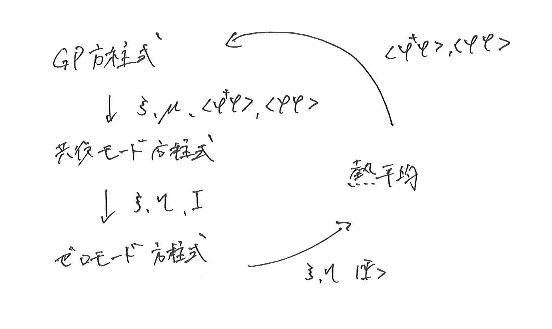
\includegraphics[width = 10cm]{self-consistent.eps}
\end{center}
\label{self-consistent}
\end{figure}
上の自己無撞着方程式が収束すると$\xi, \eta, \ket{\Psi}$が決まり, それによって分配関数$Z$や, 熱力学ポテンシャル$\Omega$を(摂動的に)求めることが可能になる. $\Omega$の摂動展開によって得られた熱力学関数は$\Omega_0$によって得られるものとは当然異なり, Zeromode-BdG間の相互作用を一部取り入れたものになっている. これを取り入れることによって上の自己無撞着ループは修正を受けるのだろうか?修正を受けるとしたらどうやってZeromode-BdGカップリングの寄与を取り込めばよいのか?

\subsection{$a(s)$の時間依存性}
相互作用描像なので演算子の時間依存性についての議論が必要. 非摂動ハミルトニアンが
\begin{eqnarray}
  H_{u, ex} = \int d\bk\ \omega_k a^\dagger(t) a(t)
\end{eqnarray}
のように対角化されていれば, 時間成分は
\begin{eqnarray}
  i\partial_ta(t) &=& [a(t), H_u] = \omega_k a(t)\\
 \therefore a(t) &=& a(0)e^{-i\omega_k t}
\end{eqnarray}
のようにくくり出せる. よって, $a^\dagger(t) a(t), a^\dagger(t) a^\dagger(t) a(t)a(t)$の時間依存性は消える. 
\subsection{$Q(s), P(s)$の時間依存性}
\newpage
\chapter{Fetter-Walecka : Quantum Theory of Many-Particle Systems(Dover, 1971)}
ちゃんと式まで書いて説明しているところもあれば, 原文の式番号だけ書いて済ませているところもあります. 原文の補助に過ぎないものだと思ってください. 
\section{Second Quantization}
だいたい知っていると思うので, Fetterの流儀を知るために簡単におさらいするに留める.
\subsection{Fields}
生成消滅演算子の線型結合について:
\begin{eqnarray}
  \hat{\psi}(\bm{x}) &\equiv& \sum_k\psi_k(\bm{x})c_k\label{2nd-quantum1}\\
  \hat{\psi}^\dagger(\bm{x}) &\equiv& \sum_k\psi_k^\dagger(\bm{x})c^\dagger_k\label{2nd-quantum2}
\end{eqnarray}
展開係数は一粒子波動関数で完全系による展開だと思えば良い\footnote{原書は ``complete set of single-particle quantum numbers'' とある. $\psi$がハミルトニアンの固有関数ならエネルギー固有関数による完全系であるし, 運動量演算子の固有関数なら運動量固有関数の完全系で展開ということになる. `` quantum numbers'' はここで言えばエネルギーか運動量か, みたいな話. }. ここで$\psi$はスピンについてのdoubletであり, $k$はなんかしらのquantum number\footnote{繰り返しになるが, 例えば主量子数・方位量子数・磁気量子数で$\bm{k} = (n, l, m)$みたいなのはよくあるよね. }:
\begin{eqnarray}
  \psi_k(\bm{x}) =
  \begin{pmatrix}
    \psi_{k1}(\bm{x})\\
    \psi_{k2}(\bm{x})
  \end{pmatrix}
  \equiv \psi_{k\alpha}(\bm{x}) & (\alpha = 1, 2)
\end{eqnarray}
$\alpha$はスピンのインデックス. $\hat{\psi}, \hat{\psi}^\dagger$は場の演算子と呼ばれる. 場の演算子は生成消滅演算子を含んでいるのでFock空間の演算子である. 場の演算子は正準交換関係を満たす:
\begin{eqnarray}
  \qty[\hat{\psi}_\alpha(\bm{x}), \hat{\psi}_\beta^\dagger(\bm{x}')]_{\mp} &=& \delta_{\alpha\beta}\delta(\bm{x} - \bm{x}')\\
  \qty[\hat{\psi}_\alpha(\bm{x}), \hat{\psi}_\beta(\bm{x}')]_{\mp} &=&\qty[\hat{\psi}^\dagger_\alpha(\bm{x}), \hat{\psi}^\dagger_\beta(\bm{x}')]_{\mp} = 0
\end{eqnarray}
$-$がボソン, $+$がフェルミオンである. 上の式はこれは生成消滅演算子の正準交換関係から得られ, 下の式は波動関数の完全性から得られる.

ハミルトニアンは場の演算子を用いて以下のように書き直せる:
\begin{eqnarray}
  \hat{H} = \int d\bm{x} \hat{\psi}^\dagger(\bm{x})T(\bm{x})\hat{\psi}(\bm{x}) + \frac{1}{2}\int\int d\bm{x}d\bm{x}' \hat{\psi}^\dagger(\bm{x})\hat{\psi}^\dagger(\bm{x}')V(\bm{x}, \bm{x}')\hat{\psi}(\bm{x}')\hat{\psi}(\bm{x})
\end{eqnarray}
$T(\bm(x))$はkinetic energy term. これがなぜハミルトニアンと呼んでよいかは山中先生の資料を参照のこと\footnote{(\ref{2nd-quantum1})(\ref{2nd-quantum2})をハミルトニアンの定義に代入すると多体量子力学のハミルトニアンが再現できる. }.

ここで一般的な一体演算子\footnote{Green関数・相関関数のような2体関数でないという意味}を考える:
\begin{eqnarray}
  J = \sum_{i = 0}^NJ(\bm{x_i})
\end{eqnarray}
なんかしらの演算子$J(\bm{x_i})$の線型結合として定義された第一量子化\footnote{第二量子化ではないというニュアンス. 第一量子化という言葉が的確かどうかは知らない. }された演算子. これを第二量子化の表示に移すと以下のようになる\footnote{(\ref{2nd-quantum3})は少々雑な議論っぽい. 運動量演算子を第二量子化したときのアナロジーが根拠か? いずれにしろ, 変換のgeneratorとして定義するほうが筋が通っているように思える. 第二量子化は場の理論よりも不完全である. }:
\begin{eqnarray}
  \hat{J} &=& \sum_{rs}\bra{r}J\ket{s}c_r^\dagger c_s\label{2nd-quantum3}\\
  &=& \int d\bm{x}\sum_{rs}\hat{\psi}^\dagger_r(\bm{x})J(\bm{x})\hat{\psi}_s(\bm{x})c_r^\dagger c_s\\
  &=& \int d\bm{x}\hat{\psi}^\dagger(\bm{x})J(\bm{x})\hat{\psi}(\bm{x})
\end{eqnarray}
以降Fetterの本では第二量子化の際はこの(\ref{2nd-quantum3})を使う. その是非はともかくとして. 

\section{Green's Functions}
このセクションではGreen関数\footnote{propagatorとかも呼ばれる}のコンセプトについて紹介する. Green関数は多体問題の取り扱いの上で重要な働きをする. 以下描像を明確にするために原書にはない添字$S, H$をつける. 
\subsection{Definition}
Green関数の定義は以下の通り:
\begin{eqnarray}
  iG_{\alpha\beta}(\bm{x}, t;\bm{x}', t') = \frac{\!_H\bra{\Psi_0}T\qty[\hat{\psi}_{H\alpha}(\bm{x}t)\hat{\psi}_{H\beta}^\dagger(\bm{x}'t')]\ket{\Psi_0}_H}{\!_H\bra{\Psi_0}\ket{\Psi_0}_H}\label{definition-green}
\end{eqnarray}
$\ket{\Psi_0}_H$は相互作用系のHeisenberg Full Hamiltonianの基底固有状態:
\begin{eqnarray}
  H_H\ket{\Psi_0}_H = E\ket{\Psi_0}_H 
\end{eqnarray}
$\hat{\psi}_{H\alpha}(\bm{x}t)$はHeisenberg描像の時間依存演算子:
\begin{eqnarray}
  \hat{\psi}_{H\alpha}(\bm{x}t) = e^{i\hat{H_H}t/\hbar}\hat{\psi}_{S\alpha}(\bm{x})e^{-i\hat{H_H}t/\hbar}
\end{eqnarray}
$\alpha\beta$は場の演算子の内部自由度であり, 今回はスピン1/2のフェルミオンを考える. T積の部分を書き下すと
\begin{eqnarray}
  T\qty[\hat{\psi}_{H\alpha}(\bm{x}t)\hat{\psi}_{H\beta}^\dagger(\bm{x}'t')] =
  \begin{cases}
    \hat{\psi}_{H\alpha}(\bm{x}t)\hat{\psi}_{H\beta}^\dagger(\bm{x}'t') & (t > t')\\
    \pm\hat{\psi}_{H\beta}^\dagger(\bm{x}'t')\hat{\psi}_{H\alpha}(\bm{x}t) & (t < t')
  \end{cases}
\end{eqnarray}
ここで符号が$+$ならボソン, $-$ならフェルミオン. つまるところ, T積は時間順序通りに演算子を並べ替えて, 演算子を入れ替えた回数を$P$とするとき, 先頭に$(-1)^P$を付ければ良い\footnote{もちろんフェルミオンの場合. ボソンの場合は$(-1)^P$因子はいらない}. というわけで, (\ref{definition-green})をexplicitに書き直すと
\begin{eqnarray}
  iG_{\alpha\beta}(\bm{x}, t;\bm{x}', t') =
  \begin{cases}
    \cfrac{\!_H\bra{\Psi_0}\hat{\psi}_{H\alpha}(\bm{x}t)\hat{\psi}_{H\beta}^\dagger(\bm{x}'t')\ket{\Psi_0}_H}{\!_H\bra{\Psi_0}\ket{\Psi_0}_H} & (t > t')\\
    \pm\cfrac{\!_H\bra{\Psi_0}\hat{\psi}_{H\beta}^\dagger(\bm{x}'t')\hat{\psi}_{H\alpha}(\bm{x}t)\ket{\Psi_0}_H}{\!_H\bra{\Psi_0}\ket{\Psi_0}_H} & (t < t')
  \end{cases}
    \label{definition-green2}
\end{eqnarray}
Green関数というのは$(\bm{x}, t), (\bm{x}', t)$にある場の演算子の期待値である\footnote{だから2点関数とか2点相関関数とかも呼ばれる}. $\ket{\Psi_0}_H$がHeisenberg Full Hamiltonianであることから演算子をSchr\"odinger描像に書き換えると
\begin{eqnarray}
  iG_{\alpha\beta}(\bm{x}, t;\bm{x}', t') =
  \begin{cases}
    e^{iE(t-t')/\hbar}\cfrac{\!_H\bra{\Psi_0}\hat{\psi}_{S\alpha}(\bm{x})e^{-i\hat{H}_H(t-t')}\hat{\psi}_{S\beta}^\dagger(\bm{x}')\ket{\Psi_0}_H}{\!_H\bra{\Psi_0}\ket{\Psi_0}_H} & (t > t')\\
    \pm e^{-iE(t-t')/\hbar}\cfrac{\!_H\bra{\Psi_0}\hat{\psi}_{S\beta}^\dagger(\bm{x}')e^{i\hat{H}_H(t-t')}\hat{\psi}_{S\alpha}(\bm{x})\ket{\Psi_0}_H}{\!_H\bra{\Psi_0}\ket{\Psi_0}_H} & (t < t')
  \end{cases}
    \label{definition-green3}
\end{eqnarray}
\subsection{Relation to Observables}
Green関数を勉強する理由はいくらかあって, そのひとつはFeynman diagramである. Feynman ruleで摂動計算をするときに場の演算子の積よりもGreen関数で表現するほうがシンプルになる. また, (\ref{definition-green})は基底固有関数で期待値を取っているため基底状態の情報がいくらか失われているのだが, 依然として興味深いオブザーバブルの特徴を保有している:
\begin{itemize}
\item 基底状態における様々な一粒子演算子の期待値
\item 基底エネルギー
\item スペクトラム
\end{itemize}
3つ目はLehmann表示で扱う\footnote{山中先生によれば, もともとは梅沢・亀淵・Lehmann表示と呼ばれていたらしい. 最近は普通にスペクトラム表示とか言う. }. 以下では上2つについて説明する.

まず一粒子演算子を考える:
\begin{eqnarray}
  \hat{J}_S &=& \int d\bm{x} {\cal \hat{J}}_S(\bm{x})\\
  \hat{{\cal J}}_S(\bm{x}) &=& \sum_{\alpha\beta}\hat{\psi}_{\beta S}^\dagger(\bm{x})J_{\beta\alpha}(\bm{x})\hat{\psi}_{\alpha S}(\bm{x})
\end{eqnarray}
$\hat{J}$は第二量子化された演算子. $J_{\beta\alpha}$は密度に関する第一量子化演算子であり$\hat{{\cal J}}$はそれを第二量子化したもの. $\ev{\hat{\cal{J}}(\bm{x})}$について:
\begin{eqnarray}
  \ev{\hat{\cal J}(\bm{x})} &=& \frac{\!_H\bra{\Psi_0}\hat{\cal J}(\bm{x})\ket{\Psi_0}_H}{\!_H\bra{\Psi_0}\ket{\Psi_0}_H} \\
  &=& \lim_{\bm{x}'\rightarrow\bm{x}}\sum_{\alpha\beta}J_{\beta\alpha}\frac{\!_H\bra{\Psi_0}\hat{\psi}^\dagger_{\beta S}(\bm{x}')\hat{\psi}_{\alpha S}(\bm{x})\ket{\Psi_0}_H}{\!_H\bra{\Psi_0}\ket{\Psi_0}_H} \\
  &=& \lim_{t'\rightarrow t^+}\lim_{\bm{x}'\rightarrow\bm{x}}\sum_{\alpha\beta}J_{\beta\alpha}\frac{\!_H\bra{\Psi_0}\hat{\psi}^\dagger_{\beta S}(\bm{x}')e^{-i\hat{H}_H(t-t')/\hbar}\hat{\psi}_{\alpha S}(\bm{x})\ket{\Psi_0}_H}{\!_H\bra{\Psi_0}\ket{\Psi_0}_H} \\
  &=& \pm i\lim_{t'\rightarrow t^+}\lim_{\bm{x}'\rightarrow\bm{x}}\sum_{\alpha\beta}J_{\beta\alpha}G_{\alpha\beta}(\bm{x}, t; \bm{x}', t')\label{before-trace}\\
  &=& \pm i\lim_{t'\rightarrow t^+}\lim_{\bm{x}'\rightarrow\bm{x}}\Tr\qty[J(\bm{x})G(\bm{x}, t; \bm{x}', t')]
\end{eqnarray}
2行目で$\bm{x}'$を登場させたり, 3行目に$\hat{1} = \lim_{t'\rightarrow t^+}e^{-iH_H(t - t')/\hbar}$を持ってきたりしたのは全てGreen関数に帰着させるためのテクニック. $G, J$は
\begin{eqnarray}
    G(\bm{x}) =
  \begin{pmatrix}
    G_{\uparrow\uparrow} & G_{\uparrow\downarrow}\\
    G_{\downarrow\uparrow} & G_{\downarrow\downarrow}
  \end{pmatrix} &  J(\bm{x}) =
  \begin{pmatrix}
    J_{\uparrow\uparrow} & J_{\uparrow\downarrow}\\
    J_{\downarrow\uparrow} & J_{\downarrow\downarrow}
  \end{pmatrix}
\end{eqnarray}
みたいな二階テンソル. これの積のトレースを取ると(\ref{before-trace})みたいになる. これが$J_{\alpha\beta}$ではなく$J_{\beta\alpha}$という表式にした理由.

例えば運動エネルギーの第一量子化は
\begin{eqnarray}
  P = -\frac{\hbar^2}{2m}\nabla^2
\end{eqnarray}
であり, これを第二量子化する:
\begin{eqnarray}
  \hat{P} &=& \int d\bm{x} \hat{{\cal P}}(\bm{x})\\
  \hat{{\cal P}}(\bm{x}) &=& \sum_{\alpha\beta}\hat{\psi}^\dagger_\beta(\bm{x})P_{\beta\alpha}\hat{\psi}_\alpha(\bm{x})\\
  \ev{P} &=& \pm i\int d\bm{x}'\lim_{\bm{x}' \rightarrow \bm{x}}\qty[-\frac{\hbar^2\nabla^2}{2m}\Tr G(\bm{x}t, \bm{x}'t^+)]
\end{eqnarray}
...工事中...
\subsection{Example : Free Fermion}
\subsection{Lehmann Representation}
この章ではフェルミオンについてのみ議論する. 状態が規格化されているものとするとGreen関数の定義は
\begin{eqnarray}
  iG_{\alpha\beta}(\bx t;\bx' t') = \!_H\bra{\Psi_0}T\qty[\psi_{H\alpha}(\bx t)\psi_{H\beta}^\dagger(\bx't)]\ket{\Psi_0}_H
\end{eqnarray}
Heisenberg描像の演算子と状態はかなり複雑だが, 面白くかつ一般的な結果を導くことができる. まず$\qty{\ket{\Psi}}$完全系を挿入:
\begin{eqnarray}
\nonumber  iG_{\alpha\beta}(\bx t;\bx' t') = \sum_n\Big\{\theta(t-t')\bra{\Psi_0}\hat{\psi}_{\alpha H}(\bx t)\ket{\Psi_n}\bra{\Psi_n}\hat{\psi}^\dagger_{\beta H}(\bx't')\ket{\Psi_0}\\
    -\theta(t'-t)\bra{\Psi_0}\hat{\psi}^\dagger_{\beta H}(\bx' t')\ket{\Psi_n}\bra{\Psi_n}\hat{\psi}_{\alpha H}(\bx t)\ket{\Psi_0}\Big\}
\end{eqnarray}
さらにSchr\"odinger描像とHeisenberg描像の変換
\begin{eqnarray}
  \hat{O}_H(t) = e^{iH_Ht/\hbar}\hat{O}_Se^{-iH_Ht/\hbar}
\end{eqnarray}
を用いて場の演算子を変換するとエネルギー固有値がくくり出せる:
\begin{eqnarray}
\nonumber    iG_{\alpha\beta}(\bx t;\bx' t') = \sum_n\Big\{\theta(t-t')e^{-i(E_n-E)(t-t')/\hbar}\bra{\Psi_0}\hat{\psi}_{\alpha S}(\bx)\ket{\Psi_n}\bra{\Psi_n}\hat{\psi}^\dagger_{\beta S}(\bx')\ket{\Psi_0}\\
    -\theta(t'-t)e^{i(E_n-E)(t-t')/\hbar}\bra{\Psi_0}\hat{\psi}^\dagger_{\beta S}(\bx')\ket{\Psi_n}\bra{\Psi_n}\hat{\psi}_{\alpha S}(\bx)\ket{\Psi_0}\Big\}
\end{eqnarray}
ここで, $\bra{\Psi_n}\hpsi\ket{\Psi_0}$について少し考えてみる. もし$\ket{\Psi_0}$が$N$個の粒子を含んでいる状態ならば, $\hpsi\ket{\Psi_0}$は$N-1$個の粒子を含む状態になるので, $\bra{\Psi_n}\hpsi\ket{\Psi_0}$が値を持つためには$\bra{\Psi_n}$が$N-1$個の粒子を含む状態でなければならない. 同様の議論から$\bra{\Psi_n}\hpsi^\dagger\ket{\Psi_0}$が値を持つためには$\ket{\Psi_n}$は$N+1$個の粒子を含む状態でなければならない. よって, $\ket{\Psi_n}$は$N\pm1$個の粒子を持つ状態である\footnote{この議論だと, 第一励起状態$\ket{\Psi_1}$, 第二励起状態$\ket{\Psi_2}$, 第三励起状態$\ket{\Psi_3}$...は全て$N\pm1$個の粒子を持つことになる. 基底だけ$N$個で残りの励起状態は全て$N\pm1$というのは少し不自然に感じる. いくらか理由を考える余地はあるが, まだ納得できる答えを持っていません. 少なくともそういう状況でなければGreen関数は値を持つことができない. }. さらに言うと, これは$\ket{\Psi_n}$が粒子数固有状態でなければならないので, BEC系のような粒子数が揺らぐ系では議論が破綻することに注意. これが, 今回Fermion系のみを考える理由である. 

ここまでの話は$\hat{H}_H$が時間非依存であるということ(と$\ket{\Psi}$が粒子数固有状態であること)を除けば一般的な議論である. このまま議論をすすめることもできるが, ここでは簡単のため運動量演算子が$\hat{H}_H$と交換する場合を考える\footnote{運動量演算子$\hat{P}$がHeisenberg Full Hamiltonian$\hat{H}_H$と交換するとき, $\hat{H}_H$の固有状態$\ket{\Psi_n}$は$\hat{P}$と同時固有状態を取るということである.}. まずは運動量演算子を並進変換のgeneratorとして導入する:
\begin{eqnarray}
  &&\hpsi_\alpha(\bx) \equiv e^{-i\hat{\bm{P}}x}\hpsi_\alpha(0)e^{i\hat{\bm{P}}x}\label{generator}\\
  \Longrightarrow&& -i\hbar\nabla\hpsi_\alpha(\bx) = \qty[\hpsi_\alpha(\bx), \hat{\bm{P}}]\\
  \Longrightarrow&& \hat{\bm{P}} = \sum_\alpha\int d\bx \hpsi^\dagger_\alpha(\bx)(-i\hbar\nabla)\hpsi_\alpha(\bx) = \sum_{\bm{k}\lambda}\hbar\bm{k}c^\dagger_{\bm{k}\lambda}c_{\bm{k}\lambda}
\end{eqnarray}
1行目を微分すると2行目になり, 2行目を満たすような$\hat{\bm{P}}$を探すと3行目になる. 3行目の2つ目のイコールは一粒子波動関数を
\begin{eqnarray}
  &&\psi_{\bm{k}\lambda}(\bx) = \frac{e^{i\bm{k}\bx}}{\sqrt{V}}\eta_{\lambda}\label{1st-plane}\\
  &&\eta_\uparrow =
  \begin{pmatrix}
    1\\
    0
  \end{pmatrix} \ \ \eta_\downarrow =
  \begin{pmatrix}
    0\\
    1
  \end{pmatrix}
\end{eqnarray}
のように平面波展開\footnote{Fourier変換のこと. 一様系だと並進対称性があり, 運動量が保存されるはず. だからハミルトニアンと運動量演算子は交換した. 先の通りハミルトニアンの固有状態は運動量固有状態にもなるので, Fourier変換してあげると運動量(c-数)が出てくる. 平面波展開はいつでもできるが, 状態がいつも運動量固有状態になっている訳はないことに注意. }して, これを式(\ref{2nd-quantum1})とかで第二量子化すれば得られる. $V$は体積. さて, この(\ref{generator})を先ほどのGreen関数の式に代入する:
\begin{eqnarray}
  \nonumber    iG_{\alpha\beta}(\bx t;\bx' t') = \sum_n\Big\{\theta(t-t')e^{-i(E_n-E)(t-t')/\hbar}e^{i\bm{P}_n\cdot(\bx - \bx')/\hbar}\bra{\Psi_0}\hat{\psi}_{\alpha S}(0)\ket{\Psi_n}\bra{\Psi_n}\hat{\psi}^\dagger_{\beta S}(0)\ket{\Psi_0}\\
    -\theta(t'-t)e^{i(E_n-E)(t-t')/\hbar}e^{-i\bm{P}_n\cdot(\bx - \bx')/\hbar}\bra{\Psi_0}\hat{\psi}^\dagger_{\beta S}(0)\ket{\Psi_n}\bra{\Psi_n}\hat{\psi}_{\alpha S}(0)\ket{\Psi_0}\Big\}
\end{eqnarray}
ここで基底状態では$\hat{\bm{P}}\ket{\Psi_0} = 0$となっていることを用いている. ここで, $G$は$\bx-\bx'$や$t-t'$にしか依存していないので$\bx-\bx' = \by$, $t-t' = s$としてFourier変換する:
\begin{eqnarray}
  G_{\alpha\beta}(\bk, \omega) &=& \int d\by\int ds\ e^{-i\bk\cdot\by}e^{i\omega s}G_{\alpha\beta}(\bx t; \bx't' )\\
\nonumber  &=& -i\int d\by ds e^{-i\bm{k}\cdot\by}e^{i\omega s}\\
\nonumber  &\times&\sum_n\Big[\ul{\theta(s)e^{-i(E_n- E)s/\hbar}e^{i\bm{P}_n\by/\hbar}\bra{\Psi_0}\hat{\psi}_{\alpha S}(0)\ket{\Psi_n}\bra{\Psi_n}\hat{\psi}^\dagger_{\beta S}(0)\ket{\Psi_0}}_{1}\\
    &&\ - \ul{\theta(-s)e^{i(E_n- E)s/\hbar}e^{-i\bm{P}_n\by/\hbar}\bra{\Psi_0}\hat{\psi}^\dagger_{\beta S}(0)\ket{\Psi_n}\bra{\Psi_n}\hat{\psi}_{\alpha S}(0)\ket{\Psi_0}}_2\Big]
\end{eqnarray}
ここで下線部1の項について計算する. $\theta$関数の積分表示
\begin{eqnarray}
  \theta(s) = -\int \frac{d\omega'}{2\pi i}\frac{e^{-i\omega' s}}{\omega' + i\eta}
\end{eqnarray}
を用いて変形していく:
\begin{eqnarray}
  \ul{ }1 &=& \frac{1}{2\pi}\sum_n\int d\by ds d\omega' e^{i(\bm{P}_n\hbar^{-1} - \bm{k})\cdot\by}e^{i(\omega - \qty(E_n - E)\hbar^{-1} -\omega')s}\frac{\bra{\Psi_0}\hat{\psi}_{\alpha S}(0)\ket{\Psi_n}\bra{\Psi_n}\hat{\psi}^\dagger_{\beta S}(0)\ket{\Psi_0}}{\omega' + i\eta}\\
  &=& \sum_n(2\pi)^3\delta(\bm{P}_n\hbar^{-1} - \bm{k})\frac{\bra{\Psi_0}\hat{\psi}_{\alpha S}(0)\ket{\Psi_n}\bra{\Psi_n}\hat{\psi}^\dagger_{\beta S}(0)\ket{\Psi_0}}{\omega - \qty(E_n - E)\hbar^{-1} + i\eta}\\
  &=& V\sum_n\delta_{\bm{P}_n\hbar^{-1},\bm{k}}\frac{\bra{\Psi_0}\hat{\psi}_{\alpha S}(0)\ket{\Psi_n}\bra{\Psi_n}\hat{\psi}^\dagger_{\beta S}(0)\ket{\Psi_0}}{\omega - \qty(E_n - E)\hbar^{-1} + i\eta}
\end{eqnarray}
最後の行でデルタ関数と体積の関係(\ref{delta-volume})を用いた. 同様の計算をすると, グリーン関数は
\begin{eqnarray}
  G_{\alpha\beta}(\bk, \omega) &=& V\sum_n\delta_{\bm{P}_n\hbar^{-1},\bm{k}}\frac{\bra{\Psi_0}\hat{\psi}_{\alpha S}(0)\ket{\Psi_n}\bra{\Psi_n}\hat{\psi}^\dagger_{\beta S}(0)\ket{\Psi_0}}{\omega - \qty(E_n - E)\hbar^{-1} + i\eta}\\ &+& V\sum_n\delta_{\bm{P}_n\hbar^{-1},-\bm{k}}\frac{\bra{\Psi_0}\hat{\psi}^\dagger_{\beta S}(0)\ket{\Psi_n}\bra{\Psi_n}\hat{\psi}_{\alpha S}(0)\ket{\Psi_0}}{\omega + \qty(E_n - E)\hbar^{-1} - i\eta}
\end{eqnarray}
となることがわかる. クロネッカーデルタが効いてくるのは$\ket{\Psi_n}$に対してなので
\begin{eqnarray}
  G_{\alpha\beta}(\bk, \omega) = V\sum_n\Big[\frac{\bra{\Psi_0}\hat{\psi}_{\alpha S}(0)\ket{n\bk}\bra{n\bk}\hat{\psi}^\dagger_{\beta S}(0)\ket{\Psi_0}}{\omega - \qty(E_n - E)\hbar^{-1} + i\eta}+ \frac{\bra{\Psi_0}\hat{\psi}^\dagger_{\beta S}(0)\ket{n, -\bk}\bra{n, -\bk}\hat{\psi}_{\alpha S}(0)\ket{\Psi_0}}{\omega + \qty(E_n - E)\hbar^{-1} - i\eta}\Big]
\end{eqnarray}
と書くことにする\footnote{ある$\bm{P}_n$に対応する$\bk$はひとつで, クロネッカーデルタなんか和を取って消えてしまうのでは?と思うかもしれない. しかし$\bk$はいくつもの準粒子のエネルギーの総和なので, $\bk$の選び方に対して同じエネルギーを持つものはいくつか存在する(縮退している?). 対して$\bm{P}_n$は$\hat{H}_H$の固有状態なので, $\ket{\Psi_n}$の縮退がなければ$\hat{P}_n$の縮退もない. そういうことで$\ket{\Psi_n}$を$n$と$\bk$でパラメトライズしている. これは一様系であるために運動量が保存し, そのquantum numberであるkを明示したに過ぎないらしい. そもそも$n$は様々なquantum numberを持っているが, 今回は$k$が保存するのでそれを外に出して$n$の定義を変えた, ということらしい. }. というわけで, これでGreen関数の周波数($\omega$)依存性を示すことができた. この分母についてもうちょっと詳細に見てみよう. 上式の第一項の分母は以下のように変形できる:
\begin{eqnarray}
  \omega - \hbar^{-1}\qty[E_n(N+1) - E(N)] = \omega - \hbar^{-1}\qty[E_n(N+1) - E(N+1)] -\hbar^{-1}\qty[E(N+1) - E(N)]
\end{eqnarray}
ここで$E(N+1) - E(N)$は基底状態に粒子が1つ追加された時のエネルギー差である. 粒子数変化に伴うエネルギー変化率をケミカルポテンシャルと呼ぶ. $E_n(N+1) - E(N+1)$は$N+1$粒子系の励起エネルギーである. そんなわけで, 書き直す:
\begin{eqnarray}
  G_{\alpha\beta}(\bk, \omega) = \hbar V\sum_n\Big[\frac{\bra{\Psi_0}\hat{\psi}_{\alpha S}(0)\ket{n\bk}\bra{n\bk}\hat{\psi}^\dagger_{\beta S}(0)\ket{\Psi_0}}{\hbar\omega -\mu - \epsilon_{n\bk}\qty(N+1) + i\eta}+ \frac{\bra{\Psi_0}\hat{\psi}^\dagger_{\beta S}(0)\ket{n, -\bk}\bra{n, -\bk}\hat{\psi}_{\alpha S}(0)\ket{\Psi_0}}{\hbar\omega -\mu + \epsilon_{n,-\bk}\qty(N-1) - i\eta}\Big]\label{green-rehmann}
\end{eqnarray}
$\eta$ に$\hbar^{-1}$がついていないが, $\eta$の定義の中に押し込めている. $\mu$も$N$依存性を持っているが
\begin{eqnarray}
  \mu(N+1) = \mu\qty(N\qty(1+\frac{1}{N})) = \mu(N) + O(N^{-1})
\end{eqnarray}
になるので, $N$が十分大きいものとして無視することにする.

これでスピン$\frac{1}{2}$の場合の$G$の行列構造についてシンプルにまとめることができた. このGreen関数は$2\times2$行列なので単位行列とPauli行列で構成される完全系で展開することができる\footnote{単に, 単位行列とパウリ行列の線型結合で書けるということ.}. 今回の問題は一様系なので指向性は無いため, $G$は空間回転に対してスカラー\footnote{ここでいうスカラーは"スカラー演算子"の意味. $\nabla = \qty(\partial_x, \partial_y, \partial_z)$はベクトル演算子, $\nabla\cdot\bk$はスカラー演算子. Pauli行列完全系も$\bm{\sigma} = \qty(\hat{\sigma}_x, \hat{\sigma}_y, \hat{\sigma}_z)$みたいなベクトル演算子だと考えれば$\bm{\sigma}\cdot\bk$もスカラー演算子である. }でなければならない. $G$には$\bm{\sigma}$と$\bk$が含まれるはずであり, $\bk$は$\bm{\sigma}$とペアになっていなければならないので
\begin{eqnarray}
  G(\bk, \omega) = a\bm{I} + b\bm{\sigma}\cdot\bk
\end{eqnarray}
という形になる. ここでハミルトニアンは空間鏡映対称性を持っており, この性質はGreen関数にも引き継がれているが, $\bm{\sigma}\cdot\bk$は擬スカラーなので鏡映対称性を持っていない. よって$b$の項は消えなければならない. これでGreen関数がとてもシンプルに書けることがわかる. (\ref{2nd-quantum1})(\ref{1st-plane})から場の演算子を平面波展開した表式
\begin{eqnarray}
  \hpsi(0) = \sum_k\frac{1}{\sqrt{V}}c_k
\end{eqnarray}
や
\begin{eqnarray}
  \epsilon_{\bk}(N+1) &=& \epsilon_{\bk}^0 - \epsilon_F^0 = \frac{\hbar^2(k^2 - k_F^2)}{2m}\\
  \mu &=& \epsilon_F^0
\end{eqnarray}
を用いるとFree FermionのGreen関数を再現できる:
\begin{eqnarray}
  G(\bk, \omega) = \delta_{\alpha\beta}\qty[\frac{\theta(k-k_F)}{\omega - \omega_k + i\eta} + \frac{\theta(k_F-k)}{\omega - \omega_k - i\eta}]
\end{eqnarray}
さて, ここで(\ref{green-rehmann})は$\hbar\omega$についての極を持つ関数である. $\epsilon_{n\bk}$が正定値なので$\Re\hbar\omega < \mu$ならば(\ref{green-rehmann})の第一項は極を持たない. 一方で$\Re\hbar\omega > \mu$ならば(\ref{green-rehmann})の第二項は極を持たない. これは原書のFig.7.1\footnote{$\hbar\omega$が複素数であることに注意. つまり, 縦軸が$\hbar\omega$の虚部, 横軸が実部.}のとおり. バッテンがGreen関数が極を持つ点を表している. 実軸よりちょっと上にあるか下にあるかは$i\eta$の符号が決めている. さて, Fig7.1を見てわかる通り, $\hbar\omega$の複素空間上では上部も下部も正則ではない. しかし, 今後の計算の上ではどちらか一方は正則であってほしい. ということで, 遅延Green関数・先進Green関数を定義する:
\begin{eqnarray}
  iG^R_{\alpha\beta}(\bx t;\bx't') &=& \bra{\Psi_0}\qty{\hpsi^\dagger_{H\alpha}(\bx t), \hpsi_{H\beta}(\bx't')}\ket{\Psi_0}\theta(t-t')\\
  iG^A_{\alpha\beta}(\bx t;\bx't') &=& \bra{\Psi_0}\qty{\hpsi_{H\beta}(\bx't'), \hpsi^\dagger_{H\alpha}(\bx t)}\ket{\Psi_0}\theta(t'-t)
\end{eqnarray}
これらは今までのGreen関数\footnote{因果Green関数という.}と同じように解析を進めることができ, 一様系でRehmann表示をしてみると
\begin{eqnarray}
  G_{\alpha\beta}^{R, A}(\bk, \omega) = \hbar V\sum_n\Big[\frac{\bra{\Psi_0}\hat{\psi}_{\alpha S}(0)\ket{n\bk}\bra{n\bk}\hat{\psi}^\dagger_{\beta S}(0)\ket{\Psi_0}}{\hbar\omega -\mu - \epsilon_{n\bk}\qty(N+1) \pm i\eta}+ \frac{\bra{\Psi_0}\hat{\psi}^\dagger_{\beta S}(0)\ket{n, -\bk}\bra{n, -\bk}\hat{\psi}_{\alpha S}(0)\ket{\Psi_0}}{\hbar\omega -\mu + \epsilon_{n,-\bk}\qty(N-1) \pm i\eta}\Big]\label{green-rehmann2}
\end{eqnarray}
となっている. 遅延Green関数の極は下部にまとまり, $\Im \omega > 0$の領域では解析的である. 先進はその逆. もし$\omega$が実なら
\begin{eqnarray}
  \qty[G_{\alpha\beta}^{R}(\bk, \omega)]^* = G_{\alpha\beta}^{A}(\bk, \omega)
\end{eqnarray}
の関係にある. 遅延と先進の違いは収束因子$i\eta$の符号のみである. もし$\omega$が実で$\hbar^{-1}\mu$より大きければ, 無限小の$i\eta$は何の役割も成さなくなる. 以上より
\begin{eqnarray}
  G_{\alpha\beta}^R(\bk, \omega) = G_{\alpha\beta}(\bk, \omega) & \Re\hbar\omega > \mu\\
  G_{\alpha\beta}^A(\bk, \omega) = G_{\alpha\beta}(\bk, \omega) & \Re\hbar\omega < \mu
\end{eqnarray}
\subsection{Physical Interpretation of the Green's Function}
一粒子Green関数の物理的な解釈を理解するために相互作用描像の状態$\ket{\Psi_I(t')}$と, $(\bx't')$に粒子を加える操作$\hpsi_{i\beta}(\bx't')\ket{\Psi_I(t')}$について考える. $\ket{\Psi_I(t')}$はハミルトニアンの固有状態ではないが, 時間発展演算子$\hat{U}(t, t')$は有効である. さて, $t>t'$において$\hat{U}(t, t')\hpsi_{I\beta}^\dagger(\bx't')\ket{\Psi_I(t')}$と$\hpsi^\dagger_{\bx t}\ket{\Psi_I(t)}$のoverlapについて考えてみる\footnote{$(\bx t)$に粒子を追加した状態と$(\bx't')$に粒子を追加して時間を$t$に合わせてあげた状態のoverlapを見ている?}:
\begin{eqnarray}
  \bra{\Psi_I(t)}\hpsi_{I\alpha}(\bx t)\hat{U}(t, t')\hpsi^\dagger_{I\beta}(\bx't')\ket{\Psi_I(t')} = \bra{\Psi_0}\hpsi_{H\alpha}(\bx t)\hpsi^\dagger_{H\beta}(\bx't')\ket{\Psi_0}
\end{eqnarray}
この計算過程でGell-Mann-Lowの定理を用いた. $\ket{\Psi_0}$はFull Hamiltonianの固有状態. これはまさに$t>t'$におけるGreen関数の定義になっており, 粒子の追加を含む状態の伝搬を特徴づけている.

この時間に関する伝搬が$G(\bk, \omega)$とどのように関係しているかを考える.

... 工事中 ...

\section{Wick's Theorem}
\subsection{概略}
前章でGreen関数の定義と性質を見た. そういうわけで, 摂動論でGreen関数を評価せねばならない. なぜならそれが相互作用描像で最も簡単な方法だから. しかしながら, Green関数は相互作用描像の基底状態によるHeisenberg演算子の期待値で定義されている. これは摂動論では不便なので, Heisenberg演算子$\hat{O}_H(t)$とそれに対応する$\hat{O}_I(t)$の関係について以下では考えることにする. ここで証明したいのは
\begin{itembox}[c]{Heisenberg演算子と相互作用演算子}
  \begin{eqnarray}
\nonumber    \frac{\ev{\hat{O}_H(t)}{\Psi_0}}{\bra{\Psi_0}\ket{\Psi_0}} &=& \frac{1}{\ev{\hat{S}}{\Phi_0}}\bra{\Phi_0}\sum_{\nu = 0}^\infty \qty(\frac{-i}{\hbar})^\nu \frac{1}{\nu !}\int_{-\infty}^\infty dt_1\cdots dt_\nu\\
&&\times e^{-\epsilon(|t_1| + \cdots + |t_\nu|)} T\qty[\hat{H}_I(t_1)\cdots\hat{H}_I(t_\nu)\hat{O}_I(t)]\ket{\Phi_0}\\
\nonumber where\hspace{0.7cm}  \hat{S} &=& U_\epsilon(\infty, -\infty)\label{wick1}
  \end{eqnarray}
\end{itembox}

これの証明はGell-Mann Lowの定理を用いる. $\ket{\Phi_0}$はFree Hamiltonianの基底状態. 同様にして
\begin{itembox}[c]{Heisenberg演算子の時間順序積と相互作用演算子}
  \begin{eqnarray}
\nonumber    \frac{\ev{T\qty[\hat{O}_H(t)\hat{O}_H(t')]}{\Psi_0}}{\bra{\Psi_0}\ket{\Psi_0}} &=& \frac{1}{\ev{\hat{S}}{\Phi_0}}\bra{\Phi_0}\sum_{\nu = 0}^\infty \qty(\frac{-i}{\hbar})^\nu \frac{1}{\nu !}\int_{-\infty}^\infty dt_1\cdots dt_\nu\\
&&\times e^{-\epsilon(|t_1| + \cdots + |t_\nu|)} T\qty[\hat{H}_I(t_1)\cdots\hat{H}_I(t_\nu)\hat{O}_I(t)\hat{O}_I(t')]\ket{\Phi_0}\label{wick2}
  \end{eqnarray}
\end{itembox}

を証明する. ここでは$\epsilon\rightarrow 0$の極限が許される\footnote{分母の$\hat{S}$行列の位相因子と分子の位相因子が$\epsilon\rightarrow 0$のもとでキャンセルする}. これにより, Green関数を
\begin{eqnarray}
  i\tilde{G}_{\alpha\beta}(x, y) = \sum_\nu^\infty \qty(\frac{-i}{\hbar})^\nu \frac{1}{\nu!}\int_{-\infty}^\infty dt_1\cdots dt_\nu\frac{\bra{\Phi_0}T\qty[\hat{H}_1(t_1)\cdots\hat{H}_1(t_\nu)\hpsi_\alpha(x)\hpsi_\beta(y)]\ket{\Phi_0}}{\bra{\Phi_0}S\ket{\Phi_0}}
\end{eqnarray}
と書くことができる. いつもの$x = (\bx, t_x)$という表記を採用. これ以降相互作用描像の添字$I$を省略する. ここで相互作用を
\begin{eqnarray}
  U(x_1, x_2) = V(\bx_1, \bx_2)\delta(t_1 - t_2)
\end{eqnarray}
とすると便利. $G_{\alpha\beta}(x, y)$の分子$\tilde{G}_{\alpha\beta}(x, y)$は
\begin{eqnarray}
\nonumber  i\tilde{G}_{\alpha\beta}(x, y) = iG^0_{\alpha\beta}(x, y) &+& \qty(\frac{-i}{\hbar})\sum_{\lambda\lambda'\mu\mu'}\frac{1}{2}\int d^4xd^4x U(x_1, x_1')\\
  &&\times \ev{T[\hpsi_{\lambda}^\dagger(x_1)\hpsi^\dagger_{\mu}(x_1')\hpsi_{\mu'}(x_1')\hpsi_{\lambda'}(x_1)\hpsi_{\alpha}(x)\hpsi^\dagger_{\beta}(y)]}{\Phi_0} + \cdots
\end{eqnarray}
のように非相互作用部$G^0$と相互作用部の積分に分解できる. つまり, 相互作用を考えるためには積分項, 特に$\ev{T[\hpsi^\dagger\cdots\hpsi\hpsi_{\alpha}(x)\hpsi^\dagger_{\beta}(y)]}{\Phi_0}$みたいな項を評価しなければならない.

明らかなのは生成演算子と消滅演算子はペアになっていなければならないこと. さもなくば期待値はゼロになる. しかしながら, 交換・反交換関係のみを用いてゼロにならない項を分類するのはとってもめんどくさい. その処方箋としてのWickの定理である. これは行列要素を評価する一般的な手続きらしい. 今後は第二量子化の際に導入したsingle mode$\qty{c_k}$ではなく, 場の演算子$\hpsi(x)$をまんま使ったほうが見通しがよい. まず, 一般に場の演算子が生成部と消滅部に分解できるとする:
\begin{eqnarray}
  \hpsi(x) = \hpsi^{(+)}(x) + \hpsi^{(-)}(x)
\end{eqnarray}
$(+)$が消滅部, $(-)$が生成部を担う.

Wickの定理を証明するためにいくつかの新しい定義を導入する.

\subsubsection{1. T積}
場の演算子についてはすでに定義した. Fermionについては定義より
\begin{eqnarray}
  T(\hat{A}\hat{B}\hat{C}\hat{D}\cdots) = (-1)^PT(\hat{C}\hat{A}\hat{D}\hat{B}\cdots)
\end{eqnarray}
となる. $P$は演算子の入れ替えの回数. 

\subsubsection{2. N積}
生成演算子を左に, 消滅演算子を右に並べ替える積. これまた入れ替えの時にはT積と同様の因子がかかる:
\begin{eqnarray}
  N(\hat{A}\hat{B}\hat{C}\hat{D}\cdots) = (-1)^PN(\hat{C}\hat{A}\hat{D}\hat{B}\cdots)
\end{eqnarray}
消滅演算子が左にあるので, Free Hamiltonianの基底状態$\ket{\Phi_0}$によるN積の期待値はゼロになる. これ重要. また分配法則も成り立つ. 

\subsubsection{3. 縮約}
$\hat{U}$と$\hat{V}$の縮約を以下のように定義する:
\begin{itembox}[c]{Contraction}
  \begin{eqnarray}
    \wick{1}{<1U >1V} = T(\hat{U}\hat{V}) - N(\hat{U}\hat{V})\label{wick3}
  \end{eqnarray}
\end{itembox}
原文の例にあるとおり, 多くの縮約はT積とN積が同じ値を取ることによりゼロになる. じゃあゼロじゃない縮約はどんなのがあるかというと原文の(8.27)みたいなやつ. これは$\ket{\Phi_0}$によるN積の期待値がゼロになることから簡単に証明できる. つまり
\begin{itembox}[c]{ContractionとGreen関数}
  \begin{eqnarray}
    \wick{1}{<1\psi >1\psi^\dagger} = iG^0_{\alpha\beta}(x, y)\label{wick4}
\end{eqnarray}
\end{itembox}

\subsubsection{4. 規約}
縮約された演算子の入れ替えは任意の演算子と同じ規則を持ち, かつ縮約はc-数なので縮約がまとまればN積の外に出すことができる:
\begin{eqnarray}
  N(\wick{1}{<1A B >1C D}) = \pm N(\wick{1}{<1A >1C B D}) = \pm \wick{1}{<1A >1C}N(BD)
\end{eqnarray}
また, 縮約の定義から$\wick{1}{<1U >1V} = \pm \wick{1}{<1V >1U}$であることもわかる. 

\subsubsection{5. Wickの定理}
原文の(8.32)のとおり. 演算子のT積はN積とあらゆる可能な縮約の和で表される.

イメージとして, T積の中で生成演算子を左にどんどん持っていくときに, 演算子が交換しない時に余分な項を生み出し, これが縮約である. 原書の(8.27)のとおり, 生成演算子が消滅演算子の左側にあると縮約は消える(ほとんどの縮約はゼロだったよね).

これを証明するために以下の補題を考える.

\subsubsection{6. 補題}
あるN積$N(UV\cdots XY)$とある演算子$\hat{Z}$の積について. $\hat{Z}$は$UV\cdots XY$よりも早い時間変数を持っている(つまり, T積では右に来る). このとき, 原書の(8.33)の式が成り立つ. 言い換えると, N積に早い時間の演算子$Z$を右から掛けたらもとからN積にあった演算子それぞれについて$Z$と縮約を取ったN積の和と, もとのN積に$Z$を加えたものの和になる. これを証明するにあたって以下の3点に注意する:\\

(a) $Z$が消滅演算子なら, T積とN積がイコールになり縮約はゼロになる. よって, 補題の右辺は最後の項しか残らず, 補題は証明される. \\

(b) N積内の$UV\cdots XY$は既に正規順序積になっていると考えて良い. つまり$UV\cdots XY = N(UV\cdots XY)$. もし正規順序積になっていなかったとしても余計に出てくる因子は左辺と右辺で打ち消し合うことになる. \\

(c) $UV\cdots XY$はすべて消滅演算子だと考えて良い. 生成演算子を含む場合も, 左から生成演算子を掛けることで議論を一般化できる. \\

この補題は演算子が2つの場合はすぐに証明ができる. ここから帰納法で補題を証明する. 補題も原書の(8.36)のような定理を用いることで証明できる.

さらにこの補題は演算子の縮約$\wick{1}{<1R >1S}$を掛けることで一般化できる. 

\subsubsection{Wickの証明}
2つの演算子については自明. 補題と同様に帰納法で証明する. 


\subsection{(\ref{wick1})}
\subsection{(\ref{wick2})}
\subsection{(\ref{wick3})の縮約ゼロについて}
たとえば
\begin{eqnarray}
  T\qty[\hpsi^{(+)}(x)\hpsi^{(-)}(y)] = \begin{cases}
    \hpsi^{(+)}(x)\hpsi^{(-)}(y) & t_x > t_y\\
    \pm\hpsi^{(-)}(y)\hpsi^{(+)}(x) & t_x < t_y
  \end{cases}
\end{eqnarray}
について. $\psi$は相互作用描像の演算子$c_ke^{-i\omega_k t}$の線型結合であり時間変数をくくり出せることからT積は意味を成さなくなる. よって$\psi$は(反)交換が可能であり
\begin{eqnarray}
  T\qty[\hpsi^{(+)}(x)\hpsi^{(-)}(y)] = \pm\hpsi^{(-)}(y)\hpsi^{(+)}(x) = N(\hpsi^{(+)}(x)\hpsi^{(-)}(y))
\end{eqnarray}
と一意に書くことができる. T積とN積の値が同じになるのでContractionはゼロになる.

\ul{なぜHeisenberg描像では成り立たないのか?}
\subsection{(\ref{wick4})}
$\ket{\Phi_0}$によるT積の期待値を計算する. 縮約の定義から:
\begin{eqnarray}
  \ev{T(UV)}{\Phi_0} = \ev{\wick{1}{<1U >1V}}{\Phi_0} + \ev{N(UV)}{\Phi_0} = \wick{1}{<1U >1V}
\end{eqnarray}
縮約はc-数なので$\ket{\Phi_0}$の外に出すことができ, $\ket{\Phi_0}$によるN積の期待値はゼロになる. 
\subsection{縮約とは?}
いきなり縮約の定義が出てきたことを不思議に思うかもしれない. そもそもはT積からスタートし,
\begin{eqnarray}
  T\qty[\hpsi(x_1)\hpsi^\dagger(x_2)] &=& \theta\qty(t_1 - t_2)\hpsi(x_1)\hpsi^\dagger(x_2) \pm \theta\qty(t_2 - t_1)\hpsi^\dagger(x_2)\hpsi(x_1)\\
  &=& \theta\qty(t_1 - t_2)\qty[\hpsi(x_1), \hpsi^\dagger(x_2)]_{\mp} \pm \hpsi^\dagger(x_2)\hpsi(x_1)\\
  &=& \theta\qty(t_1 - t_2)\qty[\hpsi(x_1), \hpsi^\dagger(x_2)]_{\mp} + N\qty(\hpsi(x_1)\hpsi^\dagger(x_2))\\
  \nonumber  where &&\theta\qty(t_2 - t_1) = 1 - \theta\qty(t_1 - t_2)
\end{eqnarray}
右辺第一項をContractionと呼ぶ. 交換関係からc-数であることは明らか. Wickの証明で「演算子が交換しない時に余分な項を生み出し」とあるが, 演算子が交換する場合右辺第一項は消えることからこれも明らか.

\subsection{補題の(b)}
例として$N(XUY)Z$を考える. $U$のみ生成演算子としてN積内を正規順序にすると
\begin{eqnarray}
  N(XUY)Z = (-1)N(UXY)Z
\end{eqnarray}
となる. これについて補題を適応すると
\begin{eqnarray}
  (-1)N(UXY)Z = (-1)\qty[N(\wick{1}{UX<1Y>1Z}) + N(\wick{1}{U<1XY>1Z})+ N(\wick{1}{<1UXY>1Z})+ N(UXYZ)]
\end{eqnarray}
となり$(-1)$の因子が打ち消されてN積内が正規順序である場合に帰着された. もっと一般的な場合も直感的に大丈夫そう. 
\subsection{補題の(c)}
Eを生成演算子として補題の左から掛ける. 生成演算子はN積の左に来る:
\begin{eqnarray}
  (左辺) = EN(UV\cdots XY)Z = N(EUV\cdots XY)Z
\end{eqnarray}
右辺についても最後の項も含めて同様に$E$を挿入することができる. つまり
\begin{eqnarray}
\nonumber  N(EUV\cdots XY)Z &=& N(EUV\cdots \wick{1}{X <1Y >1Z}) + N(EUV\cdots \wick{1}{<1X Y >1Z}) + \cdots \\
  && N(\wick{1}{E<1UVX... Y >1Z}) + N(EUV\cdots XYZ)
\end{eqnarray}
となる. これでは$N(\wick{1}{<1EUVX... Y >1Z})$の項が足りないので補題の形を満足していないが, そもそも$\wick{1}{<1E>1Z}$は生成演算子同士の縮約であることからゼロになるので$N(\wick{1}{<1EUVX... Y >1Z})$を勝手に追加しても良い. これで生成演算子があった場合でも補題を満たすことが示された. 
\subsection{演算子が2つのときの補題}
\begin{eqnarray}
  N(Y)Z = YZ = T(YZ) = \wick{1}{<1Y >1Z} + N(YZ)
\end{eqnarray}
より証明完了.

\subsection{帰納法で補題を証明}
ある消滅演算子$D$を補題の左から掛ける. $UV\cdots XY$は全て消滅演算子なので:
\begin{eqnarray}
  DN(UV\cdots XY)Z = N(DUV\cdots XY)Z
\end{eqnarray}
ここで補題を適応:
\begin{eqnarray}
\nonumber  N(DUV\cdots XY)Z &=& N(DUV\cdots \wick{1}{X <1Y >1Z}) + N(DUV\cdots \wick{1}{<1X Y >1Z}) + \cdots \\
  && N(\wick{1}{D<1UVX... Y >1Z}) + DN(UV\cdots XYZ)
\end{eqnarray}
原文の補題(8.33)に左から消滅演算子$D$を掛けても, 最後の項以外は$D$をそのままN積の中に入れてしまうことができる. なぜなら唯一の生成演算子である$Z$が縮約を取ってc-数になっているからである. ゆえに, まだ縮約を取っていない最後の項の$D$をN積の先頭に追加することは許されない. その代わりもし
\begin{eqnarray}
  DN(UV\cdots XYZ) = N(\wick{1}{<1DUV... XY>1Z}) + N(DUV\cdots XYZ)\label{wick5}
\end{eqnarray}
が成立していれば, 補題は証明できそうである. 

\subsection{補題の補題}
(\ref{wick5})について. N積の定義より
\begin{eqnarray}
  DN(UV\cdots XYZ) = (-1)^PDZUV\cdots XY
\end{eqnarray}
$P$はZをDの前まで持ってくるのに要した交換回数. さらに$Z$は$D$より早い時間を持つのでT積を挿入できる:
\begin{eqnarray}
  (-1)^PDZUV\cdots XY = (-1)^PT(DZ)UV\cdots XY  
\end{eqnarray}
T積を縮約とN積に展開:
\begin{eqnarray}
  (-1)^PT(DZ)UV\cdots XY = (-1)^P\wick{1}{<1D >1Z}UV\cdots XY + (-1)^{P+Q}N(ZD)UV\cdots XY
\end{eqnarray}
$Q$は$D$と$Z$を入れ替えたときの因子. 右辺第一項の$\wick{1}{<1D >1Z}$は既にc-数なのでN積に書き換え, 再び$Z$を一番後ろに持っていく\footnote{これは「\textbf{4. 規約}」で説明済み}:
\begin{eqnarray}
  (-1)^P\wick{1}{<1D >1Z}UV\cdots XY = (-1)^PN(\wick{1}{<1D >1Z}UV\cdots XY) = (-1)^{2P}N(\wick{1}{<1D UV... XY >1Z}) = N(\wick{1}{<1D UV... XY >1Z})
\end{eqnarray}
右辺第二項の$Z$も同様に一番後ろに持って行く:
\begin{eqnarray}
  (-1)^{P+Q}N(ZD)UV\cdots XY = (-1)^{2(P+Q)}N(DUV\cdots XYZ)= N(DUV\cdots XYZ)
\end{eqnarray}
よって(\ref{wick5})が証明できた. 
\subsection{補題の一般化}
補題に$\wick{1}{<1R >1S}$を掛ける:
\begin{eqnarray}
  \nonumber   \wick{1}{<1R >1S}N(DUV\cdots XY)Z &=& \wick{1}{<1R >1S}N(DUV\cdots \wick{1}{X <1Y >1Z}) + \wick{1}{<1R >1S}N(DUV\cdots \wick{1}{<1X Y >1Z}) + \cdots \\
  && \wick{1}{<1R >1S}N(\wick{1}{D<1UVX... Y >1Z}) + \wick{1}{<1R >1S}N(\wick{1}{<1DUV... XY>1Z}) + \wick{1}{<1R >1S}N(DUV\cdots XYZ)
\end{eqnarray}
この$\wick{1}{<1R >1S}$をN積の中に入れて正規順序になるような入れ替えを両辺で行うと, 結局両辺に同じ因子$(-1)^P$がかかることになり, $R$と$S$のラベルを$V$と$X$に入れ替えてあげれば原文の(8.38)が得られる. 
\subsection{2つの演算子のWick}
これは「演算子が2つのときの補題」と同じ. 
\subsection{帰納法でWickを証明}
補題と同じように他の任意の演算子より早い時間を持つ演算子$\Omega$を左から掛ける. ここで$\Omega$は生成・消滅を特定しない:
\begin{eqnarray}
  T(UVW\cdots XYZ)\Omega = T(UVW\cdots XYZ\Omega)
\end{eqnarray}
上式の右辺は帰納法の仮定を用いて
\begin{eqnarray}
  T(UVW\cdots XYZ)\Omega = N(UVW\cdots XYZ)\Omega + N(\wick{1}{<1U >1V}W\cdots XYZ)\Omega + N(\wick{1}{<1U V>1W}\cdots XYZ)\Omega + \cdots
\end{eqnarray}
ここで補題を使うと$\Omega$をN積の中に入れることができる. $\Omega$が一番早い時間を持ったものでなくても, それぞれの項で演算子を並べ直してあげれば大丈夫. これで, 演算子が生成部と消滅部に分けられるという仮定のもと, Wickの定理が証明できた. Wickの定理を使うのは$\bra{\Phi_0}\cdots\ket{\Phi_0}$に対してであって, 縮約していないN積を含む項は消え去る. 
\section{Diagrammatic Analysis of Perturbation Theory}
Wickの定理のおかげで
\begin{eqnarray}
  i\tilde{G}_{\alpha\beta}(x, y) = \sum_\nu^\infty \qty(\frac{-i}{\hbar})^\nu \frac{1}{\nu!}\int_{-\infty}^\infty dt_1\cdots dt_\nu\frac{\bra{\Phi_0}T\qty[\hat{H}_1(t_1)\cdots\hat{H}_1(t_\nu)\hpsi_\alpha(x)\hpsi_\beta(y)]\ket{\Phi_0}}{\bra{\Phi_0}S\ket{\Phi_0}}
\end{eqnarray}
みたいなやつが評価できるようになる. 縮約は単なるFree-field Green関数$G^0$であるので, Gは$U$と$G^0$を含む級数で表されることになる. この展開は座標空間や(一様系では)運動量空間で解析することができる. ボソンについては今回も扱いません.

\subsection{Feynman Diagrams in Coordinate Space}
Wickの定理の例として
\begin{eqnarray}
\nonumber  i\tilde{G}_{\alpha\beta}(x, y) = iG^0_{\alpha\beta}(x, y) &+& \qty(\frac{-i}{\hbar})\sum_{\lambda\lambda'\mu\mu'}\frac{1}{2}\int d^4xd^4x U(x_1, x_1')\\
  &&\times \ev{T[\hpsi_{\lambda}^\dagger(x_1)\hpsi^\dagger_{\mu}(x_1')\hpsi_{\mu'}(x_1')\hpsi_{\lambda'}(x_1)\hpsi_{\alpha}(x)\hpsi^\dagger_{\beta}(y)]}{\Phi_0} + \cdots\label{first-order-green}
\end{eqnarray}
の一次の寄与について考えてみる. noninteracting ground state $\ket{\Phi_0}$での期待値を計算するときN積は消えて場の演算子の縮約\footnote{ここでは2点相関関数のことを縮約(contraction)と呼ぶ. }のみが残る. Wickの定理は取りうる全ての縮約の和が必要であり, その縮約は$\hpsi$とその共役である$\hpsi^\dagger$によって作られるものである. (\ref{first-order-green})の一次の項は
\begin{eqnarray}
  \wick{213}{<1\psi_{\lambda}^\dagger(x_1) <2\psi^\dagger_{\mu}(x_1') >2\psi_{\mu'}(x_1') >1\psi_{\lambda'}(x_1) <3\psi_{\alpha}(x) >3\psi^\dagger_{\beta}(y)} & \cdots(A)\\
  \wick{213}{<1\psi_{\lambda}^\dagger(x_1) <2\psi^\dagger_{\mu}(x_1') >1\psi_{\mu'}(x_1') >2\psi_{\lambda'}(x_1) <3\psi_{\alpha}(x) >3\psi^\dagger_{\beta}(y)} & \cdots(B)\\
  \wick{213}{<1\psi_{\lambda}^\dagger(x_1) <2\psi^\dagger_{\mu}(x_1') <3\psi_{\mu'}(x_1') >2\psi_{\lambda'}(x_1) >1\psi_{\alpha}(x) >3\psi^\dagger_{\beta}(y)} & \cdots(C)\\
  \wick{213}{<1\psi_{\lambda}^\dagger(x_1) <2\psi^\dagger_{\mu}(x_1') >2\psi_{\mu'}(x_1') <3\psi_{\lambda'}(x_1) >1\psi_{\alpha}(x) >3\psi^\dagger_{\beta}(y)} & \cdots(D)\\
  \wick{213}{<1\psi_{\lambda}^\dagger(x_1) <2\psi^\dagger_{\mu}(x_1') >1\psi_{\mu'}(x_1') <3\psi_{\lambda'}(x_1) >2\psi_{\alpha}(x) >3\psi^\dagger_{\beta}(y)} & \cdots(E)\\
  \wick{213}{<1\psi_{\lambda}^\dagger(x_1) <2\psi^\dagger_{\mu}(x_1') <3\psi_{\mu'}(x_1') >1\psi_{\lambda'}(x_1) >2\psi_{\alpha}(x) >3\psi^\dagger_{\beta}(y)} & \cdots(F)
\end{eqnarray}
の6通り. 全ての可能な時間順序で消えない寄与を列挙することによって得られる\footnote{T積をN積とT積の真空期待値にマジ展開してN積が絡んだ項を消すということ. 山中先生の資料を参照. 確かに, めんどい. }が, この手続きは1次ですらかなり複雑. Wickはそれをかなり簡単にしてくれる. これをダイアグラムで表記するとそれぞれFig. 9.1みたいになる. 実線はcontraction $G^0$で, 波線が相互作用ポテンシャルを表している.

原書の式(9.1)の式と対応するFig. 9.1はいくつか面白い特徴がある. \\

1. $(A), (B), (D), (F)$は同時刻Green関数を持っており, ダイアグラムはそれ自体で閉じている. さて同時刻Green関数の解釈について考えてみる. 同時刻についてT積は定義されていないんだけど, そういう項が相互作用ハミルトニアン$H_1$の縮約で現れてしまう. こいつは$\hpsi^\dagger\hpsi$の形で現れる. 原書(0.2)における$n^0(\bx)$は非摂動基底状態での粒子密度であり, 相互作用系では$n(\bx)$と同じになる必要はない. $(D), (F)$は(9.2)のような項を持っており, 全粒子の最低次直接相互作用を表している. この全粒子は非相互作用基底状態を作る\footnote{フェルミの海のこと}. (C), (E)は交換相互作用を表している\footnote{Slater行列より}.\\

2. (A), (B)はdisconnected diagramsであり, 他のダイアグラムのどの線にもつながってないサブユニットを含んでいる. サブユニットの中で相互作用の効果が閉じており, 結果的にサブユニットの効果を$\tilde{G}$から取り除くことができる. これまで$\ev{\hat{S}}{\Phi_0}$は無視されてきたが, 今回はちゃんと考えてあげることにする. これは原文の(8.9)の項のうち, $\hpsi_\alpha(x)\hpsi_\beta^\dagger(y)$を除いたものにあたるので, Fig. 9.3 のような$\tilde{G}_{\alpha\beta}$の外線がないダイアグラムが出てくる. これが$\tilde{G}_{\alpha\beta}$のdisconnected diagram と約分されて消える\footnote{ちゃんと証明できてないような気がする...なんとなくわかるけど. }. これがdisconnected diagramの寄与が打ち消される理由.

原文の(8.9)は(9.3)みたいにconnectedな部分とdisconnectedな部分に分けられる. $\nu$についてはクロネッカーデルタがあるので$\mu = n + m$となる. 後ろのdisconnectedな積分は$\ev{\hat{S}}{\Phi_0}$と約分されて消える. 結果, (9.5)みたいなすっきりとした形になる.

さて, これからFeynman diagramと摂動級数の関係を導出する. しかし, Feynman ruleは相互作用ハミルトニアン$H_I$に依存することを強調しておかなければならない. 今回は2体ポテンシャルを通して相互作用する同種粒子系を考える. \\

3. まず, ダイアグラムの形が同じであれば, 相互作用ハミルトニアンの添字のラベルが異なっていても$G$への寄与は同じ\footnote{dummy indexが違うだけだから. }. 加えてそいつらの符号も同じである. なぜなら$H_I$に含まれる演算子の数が偶数であり, $H_I$は自由に動かせるから\footnote{$(-1)^P$の因子が打ち消す}. 摂動$m$次ではラベルが違うだけで同じダイアグラムが$m!$個出てくるが, 原文(9.5)の$(m!)^{-1}$の因子で打ち消されることになるので, 結局同じ形のダイアグラムは1回数えればいい\footnote{この結果はconnected diagramについてのみ正しいらしい. }.

..工事中..\\

(a) $n$本の相互作用線と$2n + 1$本の方向を持つGreen関数$G^0$を用いて書けるダイアグラムを列挙する.\\

4. 1次では$C$と$E$は同じで, $D$と$F$も同じ. 異なるのは$x$と$x'$のラベルだけ. この置換えはポテンシャルが対称な場合. ダイアグラムは1種類だけ数えればよく, 原文(9.1)の$1/2$の因子はオミットできる.
ここで追加のルールを得る:\\

(b) バーテックスを4次元空間$x_i$でラベリングする. 

(c) $y\rightarrow x$の向きに進む実線は$G_{\alpha\beta}^0$を表す.

(d) 波線は相互作用を表す.

(e) 全ての空間と時間について積分する.\\

5. Green関数とポテンシャルにある添字の和は, fermion lineに沿って走る行列積の式にある. このことより次のルールが生まれる:\\ 

(f) fermion lineに沿ったスピン行列の積が存在し, 各バーテックスにポテンシャルを含んでいる\\

6. ダイアグラムの符号は次のように決まる:\\

それぞれの時刻でfermion lineが閉じていたら$-$の符号がつく. \\

(g) 各項に$(-1)^F$をつける. Fは閉じたループの数. \\

7. (9.5)式の$n$次には$(-i/\hbar)^n$がついており, $2n+1$組の縮約には$(i)^{2n+1}$がつくことから\\

(h) $G$の$n$次を計算するときは, $(i/\hbar)^n$をつける. \\

最後に(9.2)の議論から\\

(i) 同時刻のGreen関数は$G_{\alpha\beta}(\bx, t; \bx', t^+)$としましょう.

\subsection{Feynman Diagrams in Momentum Space}
原理的に, 任意のオーダーで各ダイアグラムはGreen関数に書き換えることができる. しかし, non-interacting Green関数のそれぞれが, 2つの繋がっていないピース\footnote{$G(x, y)$の$x$と$y$はそれぞれ$\hpsi(x)$と$\hpsi^\dagger(y)$のようにバラバラなピースからできている. これをFourier変換すると$G(k)$のように1変数になり, 言わば対角的になる. }で出来ていることから, 実際の期待値は厄介な問題を抱えている. 原書(9.6)の一次の寄与でさえ, 時間変数の相対値によって多くのピースに分かれてしまう. 対照的に, 時間のFourier変換によって得られる$G^0(\bx, \by, \omega)$はシンプルな形をしており, 計算に用いるのに便利である. $G_{\alpha\beta}(\bx, \bx', \omega)$を考えることもできるが, 時間非依存のハミルトニアンを持つ非一様系に適応することになる. ということで, 今は一様系でかつ空間等方は系に議論を限定する. ここではGreen関数は$\delta_{\alpha\beta}G(x-y)$という形を取る. 一様系なのでFourier変換が許され,
\begin{eqnarray}
  G_{\alpha\beta}(x, y) &=& (2\pi)^{-4}\int d^4ke^{ik(x-y)}G_{\alpha\beta}(k)\\
  G^0_{\alpha\beta}(x, y) &=& (2\pi)^{-4}\int d^4ke^{ik(x-y)}G^0_{\alpha\beta}(k)
\end{eqnarray}
熱力学極限$V\rightarrow\infty$は既に取っているものとする. ここでは4次元のnotationを採用している:
\begin{eqnarray}
  d^4k \equiv d^3kd\omega\hspace{1.0cm}k\cdot x \equiv \bk\cdot\bx - \omega t
\end{eqnarray}
さらに相互作用は座標にのみ依存するとする:
\begin{eqnarray}
  U(x, x') = V(\bx, \bx')\delta(t-t')
\end{eqnarray}
これも運動量表示で
\begin{eqnarray}
\nonumber  U(x, x')_{\alpha\alpha', \beta\beta'}(x, x') &=& (2\pi)^{-4}\int d^4ke^{ik(x-y)}U(k)_{\alpha\alpha', \beta\beta'}\\
  &=& (2\pi)^{-3}\int d^3ke^{i\bk\cdot(\bx-\by)}U(\bk)_{\alpha\alpha', \beta\beta'}\delta(t-t')
\end{eqnarray}
また
\begin{eqnarray}
  U(k)_{\alpha\alpha', \beta\beta'} = V(\bk)_{\alpha\alpha', \beta\beta'} = \int d^3xe^{-i\bk\cdot\bx}V(\bx)_{\alpha\alpha', \beta\beta'}
\end{eqnarray}
原書Fig. 9.7bのGreen関数を運動量表示に書き換えると原書(9.12)みたいになる. Green関数が2点じゃなくて1点に書き換えられた. k-表示されたGreen関数でもx-表示の時と同じようにFeynmanルールが存在する.
\subsection{Dyson's Equation}
\subsubsection{0. General derivation of Dyson's Equation}
まずは一般的なDyson方程式の導出について. ハミルトニアンが
\begin{eqnarray}
  H = \int dx\hpsi^\dagger(x) h(x)\hpsi(x) + \frac{1}{2}\int dxdx'\hpsi^\dagger(x)\hpsi^\dagger(x')U(x, x')\hpsi(x')\hpsi(x)
\end{eqnarray}
があるとする. また, スピンの添字$\alpha, \beta$は省略し, $x = (\bx, t), x' = (\bx', t)$としている. これのHeisenberg方程式は
\begin{eqnarray}
 && i\partial_t\hpsi(x) = \qty[\hpsi, H] = h(\bx)\hpsi(x) + \int dx'\hpsi^\dagger(x')U(x, x')\hpsi(x')\hpsi(x)\\
 %&\therefore& \qty[i\hbar\partial_t - h(x) - \int dx'\hpsi^\dagger(x')U(x, x')\hpsi(x')]\hpsi(x) = 0
\end{eqnarray}
遅延Green関数を
\begin{eqnarray}
  iG^R(\bx, t; \bx', 0) = \ev{\qty{\hpsi(\bx, t), \hpsi^\dagger(\bx', 0)}}{\Psi_0}\theta(t)
\end{eqnarray}
とすると, これの時間発展は
\begin{eqnarray}
\nonumber  i\partial_tG^R(\bx, t; \bx', 0) &=& \ev{\qty{\partial_t\hpsi(\bx, t), \hpsi^\dagger(\bx', 0)}}{\Psi_0}\theta(t) + \ev{\qty{\hpsi(\bx, t), \hpsi^\dagger(\bx', 0)}}{\Psi_0}\partial_t\theta(t)\\
\nonumber  &=& -i\ev{\qty{h(x)\hpsi(x) + \int dx''\hpsi^\dagger(x'')U(x, x'')\hpsi(x'')\hpsi(x), \hpsi^\dagger(\bx', 0)}}{\Psi_0}\theta(t)\\
\nonumber&& + \ev{\qty{\hpsi(\bx, t), \hpsi^\dagger(\bx', 0)}}{\Psi_0}\delta(t)\\
\nonumber  &=&h(\bx)G^R(\bx, t; \bx', 0) -i\theta(t)\int dx''U(x, x'')\ev{\qty{\hpsi^\dagger(x'')\hpsi(x'')\hpsi(x), \hpsi^\dagger(\bx', 0)}}{\Psi_0}\\
\nonumber&& +\delta(\bx-\bx')\delta(t)\\
\nonumber\qty[i\partial_t -h(\bx)]G^R(\bx, t; \bx', 0) &+&i\theta(t)\int dx''U(x, x'')\ev{\qty{\hpsi^\dagger(x'')\hpsi(x'')\hpsi(x), \hpsi^\dagger(\bx', 0)}}{\Psi_0}  = \delta(\bx-\bx')\delta(t)\\
\end{eqnarray}
左辺第二項目を
\begin{eqnarray}
\nonumber  i\theta(t)\int dx''U(x, x'')\ev{\qty{\hpsi^\dagger(\bx'', t)\hpsi(\bx'', t)\hpsi(\bx, t), \hpsi^\dagger(\bx', 0)}}{\Psi_0} = -\int dx''\int dt''\Sigma(\bx, \bx''; t - t'')G^R(\bx'', t''; \bx', 0)\\
\end{eqnarray}
という形で書くことでSelf-energy $\Sigma(\bx, \bx; t)$を定義する. 結局遅延Green関数の時間発展方程式は
\begin{eqnarray}
  \qty[i\partial_t -h(\bx)]G^R(\bx,\bx';t) -\int dx''\int dt''\Sigma(\bx, \bx''; t - t'')G^R(\bx'', t''; \bx', 0)= \delta(\bx-\bx')\delta(t)
\end{eqnarray}
さて, ここで前節でやったようにGreen関数, Self-energy, デルタ関数を
\begin{eqnarray}
  G^R(\bx, \bx';t) &=& (2\pi)^{-4}\int d\bk d\omega e^{i\bk\cdot(\bx-\bx')}e^{-i\omega t}G(\bk, \omega)\\
  \Sigma(\bx, \bx';t) &=& (2\pi)^{-4}\int d\bk d\omega e^{i\bk\cdot(\bx-\bx')}e^{-i\omega t}\Sigma(\bk, \omega)\\
  \delta(\bx - \bx')\delta(t) &=& (2\pi)^{-4}\int d\bk d\omega e^{i\bk\cdot(\bx - \bx')}e^{-i\omega t}
\end{eqnarray}
のようにFourier変換する. これで微分などが処理できる:
\begin{eqnarray}
\nonumber  &&\int d\bk d\omega \qty[\qty(\omega - k^2)e^{i\bk\cdot(\bx-\bx')}e^{-i\omega t}G(\bk, \omega) - \Sigma(\bk, \omega)e^{i\bk\cdot(\bx-\bx')}e^{-i\omega t}G(\bk, \omega)]= \int d\bk d\omega e^{i\bk\cdot(\bx - \bx')}e^{-i\omega t}\\
   &\therefore& \qty(\omega - k^2)G(\bk, \omega) - \Sigma(\bk, \omega)G(\bk, \omega)= 1\label{dyson-k}
\end{eqnarray}
ここで無次元化のことを考えると$\omega\rightarrow\hbar\omega, k^2\rightarrow \frac{\hbar^2k^2}{2m}\equiv\epsilon_k$なので,
\begin{eqnarray}
  G(\bk, \omega) = \frac{1}{\hbar\omega - \epsilon_k - \Sigma(\bk, \omega)}
\end{eqnarray}
が求まる. (\ref{dyson-k})の右辺は1になったが, 本来はスピンの足があることを考えると$\delta_{\alpha\beta}$になるべき. それで原文の(9.33)みたいになる.

\subsubsection{1. Self-energy insertion}
Green関数$G$の構造は, 非摂動Green関数$G^0$と$G^0$がたくさんconnectした項の和になっている. Fig. 9.12 は例えばGreen関数の摂動1次のまでの展開を考えるとわかりやすい. 摂動2次以上を考えるともっといろんなダイアグラムが出てきそうだけど, 1次も含めたそれらの寄与をSelf-energyに押し付けることでFig. 9.12 のような表現になる. Fig. 9.12 に対応するGreen関数は原文(9.25).

ここで「properなself-energyの挿入」という概念を導入する. properなself-energyの挿入とは, 1本の粒子線を切って2つのtermに分けられないようなself-energyの挿入をproperであるという. 原文のFig. 9.8 を例にすると, $(a), (b), (c), (d)$は$x, y$を除くvertexを切断することにより2つの部分に分けることができるが, それ以外はできない. 定義より, proper self-energyはproper self-energy insertionの全ての和になっている. proper self-energy $\Sigma(x, x')$のproper Self-energy insertion $\Sigma^\star(x, x')$による表現は原文(9.26)のとおり. (9.26)のダイアグラムがFig. 9.13. self-energyの展開(9.26)をGreen関数のself-energy表現(9.25)に代入すると(9.27)になる. これをDyson方程式と呼ぶ.
\newpage
\end{document}

